\documentclass[12pt, a4paper]{article}

% Packages
\usepackage[utf8]{inputenc}
\usepackage[T1]{fontenc}
\usepackage{amsmath, amssymb}
\usepackage{graphicx}
\newcommand*\rot{\rotatebox{90}}
\usepackage{hyperref}
\usepackage{geometry}
\usepackage{booktabs}
\usepackage{caption}
\usepackage{subcaption}
\usepackage{enumitem}
\usepackage{titlesec}
\usepackage{float}
\usepackage{setspace}
\usepackage{times}  % Times New Roman
\usepackage{rotating}
\usepackage[backend=biber, style=authoryear, natbib=true]{biblatex}
\addbibresource{../data/bibliography/references.bib} 

% Margins: 2cm all around
\geometry{
    a4paper,
    top=2cm,
    bottom=2cm,
    left=2cm,
    right=2cm
}

% Line spacing: 1.15
\setstretch{1.15}

% Rest of your preamble (tocdepth, secnumdepth, etc.)
\setcounter{tocdepth}{4}
\setcounter{secnumdepth}{4}


\title{Master Thesis Proposal: Global Cross-Asset Machine Learning Models for Forex Trading: A Nested Tournament Framework for Benchmarking Architectures and Mitigating Overfitting via Meta-Labeling, Conformal Filtering, and Statistical Discovery Control}
\author{Adam Elias Scheuerlein}
\date{\today}

\begin{document}

\maketitle
\thispagestyle{empty}  % Remove page number from the title page

\pagebreak

% Use roman numerals for front matter
\pagenumbering{roman}
\setcounter{page}{1}

\begin{abstract}
To summarize the current progress of the project as well as provide a glimpse into the planned research.
\end{abstract}

\pagebreak

% Table of Contents
\tableofcontents

\pagebreak

% List of Figures
\listoffigures

\pagebreak

% List of Tables  
\listoftables

\pagebreak

%%%%%%%%%%%%%%%%
% INTRODUCTION %
%%%%%%%%%%%%%%%%
% Switch to arabic numbers starting from here
\pagenumbering{arabic}
\setcounter{page}{1}

\section{Introduction}
\subsection{Quantifying the Unknown}

The fundamental challenge of modern quantitative finance is not a scarcity of information, but a crisis of statistical validity.
In the intraday Forex market, a domain characterized by extreme non-stationarity and a vanishingly low
signal-to-noise ratio, the traditional tools of predictive modeling often become instruments of self-deception.
When a machine learning model is tasked with finding patterns in a random walk with drift, it will invariably succeed in
finding something. The question is whether that "something" is a structural property of the market or merely a ghost in the data.

\medskip

This thesis proceeds from the premise that the path to robust algorithmic trading lies not in the optimization of predictive power,
but in the rigorous quantification of uncertainty. Most contemporary trading frameworks suffer from
a form of epistemic arrogance, the sin of being overconfident about the reliability of your own knowledge,
for they treat financial time-series as a standard supervised learning problem.
Thus, they ignore the fact that the underlying distribution of the data can shift within minutes.
To trade successfully is not necessarily to predict the future, but to establish a verification gauntlet
that can distinguish between a high-probability regime and a chaotic one.

\medskip

At the heart of this research is a shift from point-estimate trading to meta-verification.
We introduce a hierarchical architecture where every trade signal is subjected to a secondary statistical referee.
By utilizing conformal prediction, we move away from raw probabilities and toward a framework of valid inference,
where a signal is only acted upon if it meets a mathematically rigorous significance threshold.
This effectively transforms the trading system from a simple classifier into a skeptical agent, 
one that prioritizes the avoidance of false discoveries over the pursuit of frequent, but unverified, opportunities.


\subsection{Problem Statement}

The central challenge of intraday Forex trading lies in the fundamental tension between the vanishingly low signal-to-noise ratio of 
financial time series and the non-stationary nature of global market regimes.
While modern machine learning architectures possess the theoretical capacity to map these complex dynamics, 
their transition from controlled backtests to live liquidity is typically compromised by a sequence of systemic failures.
This process often begins with the data-mining trap, where the high dimensionality of feature sets and 
exhaustive hyperparameter optimization allow a model to inadvertently discover stochastic flukes rather than systematic alpha.
These overfitted strategies appear spectacular in historical simulations but remain structurally fragile, 
as their performance is a function of historical luck rather than predictive permanence.

\medskip

This fragility is further intensified by the hard classification threshold inherent in standard classifiers.
By treating every trade signal with equal weight, most models remain blind to their own uncertainty, forced to take a binary stance
even when the underlying market conditions are chaotic or ambiguous. 
Without a secondary layer of statistical skepticism, a mechanism to rigorously veto low-conviction signals through meta-verification, 
a strategy is inevitably eroded by the cumulative costs of trading in high-entropy regimes.

\medskip

Finally, even when a signal is valid, trading systems often suffer from regime blindness, a failure to account for the radical heterogeneity across currency pairs. 
A global model that performs admirably on the deep liquidity of G10 Majors may find itself catastrophically misaligned when applied to the 
idiosyncratic volatility of Emerging Markets.
Without adaptive, pair-specific execution guardrails that can adjust to local liquidity profiles, a model remains a
generalist in a market that demands specialized precision, ultimately leading to alpha decay where theoretical alpha vanishes upon contact with reality.


\subsection{Research Objectives}

The primary objective of this research is to answer the fundamental question of machine learning in algorithmic trading: 
\textbf{Can we build an ML classifier that can drive a Forex trading model successfully?}
This overarching goal is pursued by identifying which "machinery" is most effective, which components are useless or dangerous, 
and the underlying reasons for feature performance. This is decomposed into the following specific research objectives:

\begin{enumerate}
  \item \textbf{Architecture Efficacy \& The Tournament Framework}
  \begin{enumerate}
    \item \textit{Question:} How do different ML models rank and is there a clear architecture that outperforms the rest 
    when validated through a nested, purged, and embargoed walk-forward framework?
    \item \textit{Objective:} To determine which ML architectures provide the most robust framework for intraday FX data.
  \end{enumerate}
  

  \item \textbf{Efficacy of the "Meta-Machinery" (Filtering \& Sizing)}
  \begin{enumerate}
    \item \textit{Question:} Can a secondary "referee" model (M2) effectively veto low-probability trades from the primary model (M1), 
    and does conformal prediction provide a statistically superior threshold for this veto compared to simple probability cut-offs?
    \item \textit{Objective:} To quantify the value added by meta-labeling and conformal filtering.
  \end{enumerate}


  \item \textbf{Statistical Discovery Control \& Overfitting Mitigation}
  \begin{enumerate}
    \item \textit{Question:} Can the Deflated Sharpe Ratio (DSR) prevent the deployment of over-optimized models?
    \item \textit{Objective:} To distinguish between strategy luck and systematic alpha using advanced metrics.
  \end{enumerate}
  

  \item \textbf{Feature Anatomy: What Works and Why?}
  \begin{enumerate}
    \item \textit{Question:} Which features provide more stable signals and why could that be?
   \item \textit{Objective:} To perform a "post-mortem" on feature importance.
  \end{enumerate}
  

  \item \textbf{Global Robustness vs. Local Adaptation}
  \begin{enumerate}
    \item \textit{Question:} Is it more effective to have a single model architecture trained on all pairs 
    or does the model require pair-specific "execution guardrails" (ATR-based SL/TP and conformal significance levels) 
    to survive across diverse currency pairs (Majors vs. EMs)?
    \item \textit{Objective:} To evaluate the success of a "global model, local parameters" strategy.
  \end{enumerate}
\end{enumerate}


%%%%%%%%%%%%%%%%%%%%%
% LITERATURE REVIEW %
%%%%%%%%%%%%%%%%%%%%%
\section{Literature Review}

\subsection{Structural Rigor in Financial Machine Learning: Labeling, Filtering, and Validation Protocols}\label{sec:label_filter_validate}

Labeling methods such as the fixed-time horizon method fail to capture the path-dependent nature of real-world trading where a position might hit a stop-loss 
before reaching its daily close. As argued by \textcite{lopez_de_prado_advances_2018}, financial labels should instead be defined by the first of three barriers hit: 
a profit-taking level (upper), a stop-loss level (lower), or a time-expiration (vertical). It should be clear that the we label an observation with 1 (long) if the upper
barrier is hit first and with -1 (short) if the lower barrier is hit first. For the last case, when the vertical barrier is hit first, \textcite{lopez_de_prado_advances_2018}
describes two choices: the sign of the return at that time or 0 (hold). The triple-barrier method we use in this research assigns the sign of the return if the vertical
barrier is hit first and thus gives the following labeling rules:

\begin{equation}
y_i = \begin{cases}
1 & \text{if } \underbrace{t_{i, TP} < t_{i, SL} \text{ and } t_{i, TP} \leq t_i + h}_{\text{Profit Barrier Hit First}} \\
-1 & \text{if } \underbrace{t_{i, SL} < t_{i, TP} \text{ and } t_{i, SL} \leq t_i + h}_{\text{Loss Barrier Hit First}} \\
\operatorname{sgn}(r_{t_i, t_i+h}) & \text{if } \underbrace{\min(t_{i, TP}, t_{i, SL}) > t_i + h}_{\text{Vertical Barrier (Time-out) Hit}}
\end{cases}
\label{eq:tbm_binary}
\end{equation}

where \( h \) defines the expiration limit, \( t_{i, TP} \) the timestamp of observation \( i \) at which the take-profit was triggered, 
\(t_{i, SL} \) the timestamp of observation \( i \) at which the stop-loss was triggered, and \( t_i \) the current time at observation \( i \).
Adopting the triple-barrier method as the foundational labeling scheme for the primary model (M1) ensures that signal generation is 
strictly aligned with the dynamic volatility of the market.

\medskip

Building upon the path-dependent labels of the triple-barrier method, the literature identifies a fundamental distinction between predicting the 
"side" of a trade and the assessment of its "size" or reliability. \textcite{lopez_de_prado_advances_2018} argues that while practitioners often have a 
primary exogenous model to decide the market direction, they frequently lack a formal mechanism to determine whether to risk capital on a specific bet. 
To address this, he proposes the meta-labeling framework, which involves building a secondary machine learning model (M2) that learns how to 
effectively use a primary model (M1). The primary model is tasked with determining the "side" (long or short), 
while the secondary model is trained to decide whether to "take the bet" or "pass". 
This transforms the meta-model's objective into a binary classification problem:

\begin{equation}
y_i^{\text{M2}} = \begin{cases}
1 & \text{if } \hat{y}_i^{\text{M1}} = y_i \quad \text{(Correct Prediction)} \\
0 & \text{if } \hat{y}_i^{\text{M1}} \neq y_i \quad \text{(Incorrect Prediction)}
\label{eq:meta_label}
\end{cases}
\end{equation}

where \( \hat{y}_i^{M1} \) represents the side predicted by the primary model and \( y_i \) is the actual market outcome as defined by the triple-barrier method. 
This approach is particularly effective for maximizing the F1-score of a strategy by configuring the primary model for high recall to ensure it 
identifies the majority of potential positives such that the secondary model can then correct for low precision by filtering out false positives. 
As noted by \textcite{lopez_de_prado_advances_2018}, this decoupling not only limits the risk of overfitting, as the machine
learning algorithm is not tasked with learning the market direction from scratch, 
but also ensures more robust outcomes by focusing the secondary model solely on the critical decision of signal reliability.

\medskip

Beyond the design of labels and meta-filters, the architectural integrity of a trading strategy depends on the methodology used to simulate out-of-sample performance. 
\textcite{lopez_de_prado_advances_2018} distinguishes between two primary backtesting philosophies: 
the walk-forward (WF) method, which performs a historical simulation of how a strategy would have performed in the past, 
and the combinatorial purged cross-validation (CPCV) method, which simulates scenarios that did not necessarily occur in the historical sequence. 
The WF approach is favored for its clear historical interpretation and its adherence to the "filtration" of time, 
where each decision is based strictly on trailing data to guarantee a true out-of-sample test. 
However, \textcite{lopez_de_prado_advances_2018} warns that the traditional WF method suffers from the "single-path" limitation, 
making it susceptible to overfitting the specific sequence of historical events. 
To address this, he proposes the CPCV method, which generates multiple backtest paths \( \varphi \) by partitioning data into N groups and testing all possible combinations, 
thereby deriving a distribution of Sharpe ratios rather than a single, potentially volatile estimate.

\medskip

This research utilizes a nested walk-forward validation framework as the primary evaluation protocol. 
While the CPCV method presents a compelling alternative for stress-testing and defeating overfitting through scenario generation,
this study prioritizes the preservation of the temporal ordering and the historical accuracy inherent in the walk-forward approach. 
To mitigate the risk of information leakage the framework incorporates the concept of purging as defined by \textcite{lopez_de_prado_advances_2018} 
but leaves out embargoing because in the walk-forward approach the training set always predates the testing set. 
Specifically, any training observation \( i \) is purged if its evaluation interval \( \left[ t_i, t_i + h_i \right] \) 
overlaps with a test observation \( j \), ensuring that the features of the training set do not contain information about the labels in the testing set:

\begin{equation}
I_{\text{purged}} = \{\, i : (t_j \leq t_i \leq t_j + h_j) \text{ or } (t_j \leq t_i + h_i \leq t_j + h_j) \,\}
\label{eq:purging}
\end{equation}

By nesting this purged walk-forward loop within a hyperparameter optimization study (Optuna), 
the research ensures that model selection and trading parameter tuning are conducted with the highest degree of statistical rigor, 
even as it acknowledges that future extensions could benefit from the multi-path analysis offered by the CPCV framework.


\subsection{The Risk of Backtest Overfitting}\label{sec:backtest_overfitting}

The exhaustive search for profitable trading rules through automated optimization engines inevitably leads to finding 
lucky configurations that appear significant in backtests but fail in live execution. 
\textcite{bailey_deflated_2014} warn that traditional performance metrics like the Sharpe ratio 
are fundamentally misleading when reported without accounting for the number of trials conducted (\(N\)), 
as the probability of backtest overfitting increases monotonically with the volume of configurations tested. 
This research addresses this risk by implementing a verification layer that treats the results of the Optuna hyperparameter optimization 
not as deterministic facts, but as a multiple-testing problem that requires statistical deflation.
The statistical quantification of this overfitting risk requires moving beyond simple point estimates toward a probabilistic framework 
that accounts for both the distribution of returns and the selection process. 
\textcite{bailey_sharpe_2012} proposed the probabilistic Sharpe ratio (PSR), which adjusts the observed Sharpe ratio (\(\widehat{SR}\)) 
for non-normality (skewness \(\gamma_3\) and kurtosis \(\gamma_4\)) and the track record length (\(T\)):

\begin{equation}
\text{PSR}(SR^*) = \Phi \left[ \frac{(\widehat{SR} - SR^*) \sqrt{T-1}}{\sqrt{1 - \gamma_3 \widehat{SR} + \frac{\gamma_4 - 1}{4} \widehat{SR}^2}} \right]
\label{eq:psr}
\end{equation}

where \(\Phi\) is the CDF of the standard normal distribution and \(SR^*\) is the benchmark. A PSR below $50\%$ suggests that the estimated Sharpe ratio would 
not be considered statistically distinguishable from zero. To correct for the data mining trap, \textcite{bailey_deflated_2014} introduced the deflated Sharpe ratio (DSR), 
which is essentially the PSR calculated by setting the benchmark \(SR^*\) to the expected maximum Sharpe ratio found by chance 
across \(N\) trials:

\begin{equation}
SR^* = \sqrt{\text{Var}[\{SR_n\}]} \left( (1-\gamma) \Phi^{-1}\left(1 - \frac{1}{N}\right) + \gamma \Phi^{-1}\left(1 - \frac{1}{Ne}\right) \right)
\label{eq:sr_star}
\end{equation}

where \(\gamma \approx 0.5772\) is the Euler-Mascheroni constant and \(\text{Var}[\{SR_n\}]\) is the variance of the Sharpe ratios across all trials and 
thus \( \text{DSR} \equiv \text{PSR}(SR^*) \). 


\subsection{Uncertainty Quantification in Machine Learning}\label{sec:conformal_preds}

The low signal-to-noise ratio inherent in high-frequency Forex data makes the task of distinguishing true predictive signals 
from random market fluctuations a primary challenge for the quantification of uncertainty in Machine Learning.
As argued by \textcite{lopez_de_prado_advances_2018}, a simple, single-layer classification model is rarely sufficient in these domains 
because the low signal-to-noise ratio prevents a single model from simultaneously learning the "side" (directional bet) and 
the "size" (statistical conviction) of a trade without overfitting to noise. 
To solve this, \textcite{shafer_tutorial_2008} argue that the strength of conformal prediction lies in its ability to provide a measure of
confidence for every individual prediction based on how well it fits with past examples. 
This allows for the generation of confidence sets rather than mere point estimates and defines the conformal prediction \( p \)-value for a new
observation as:

\begin{equation}
p = \frac{\left\|\{i = 1, \ldots, k : \alpha_i \geq \alpha_{\text{new}}\}\right\| + 1}{k + 1}
\label{eq:conformal_p}
\end{equation}

where \( k \) is the size of the calibration set, \( \alpha_i \) represents the non-conformity measure for the 
\( i \)-th calibration point, and \( \alpha_{\text{new}} \) is the non-conformity score for the new observation.
In this research, the non-conformity score for the M2 meta-model is defined as:

\begin{equation}
\alpha = \hat{P}_{\text{M2}}(\text{Signal is Correct})
\label{eq:nonconformity}
\end{equation}

where \( \hat{P}_{\text{M2}}(\cdot) \) denotes the predicted probability from the M2 model, 
which describes whether the primary (M1) model's directional bet matches the actual market outcome.
This link transforms raw, uncalibrated success probabilities into statistically valid \( p \)-values, 
allowing for a conformal veto of M2 where a trade is only executed if its \( p \)-value exceeds a significance threshold \( \varepsilon \), effectively identifying
and filtering out "non-conforming" outliers, signals that are statistically likely to result in a mistake.


%%%%%%%%%%%%%%%
% METHODOLOGY %
%%%%%%%%%%%%%%%
\newpage

\section{Methodology}

\subsection{Overview}

Given the multi-layered and technically demanding nature of the machine learning pipeline this section provides a high-level roadmap 
of the research framework, serving as a "beacon" for the reader to return to for consultation. 
The research methodology is visually summarized through two lenses:

\begin{itemize}
    \item Figure \ref{fig:methodology flowchart} illustrates the end-to-end project lifecycle. 
    It begins with the ingestion and preparation of raw data, continues with a model tournament, 
    and ultimately crowns a tournament winner which is made ready for production.

    \item Figure \ref{fig:pipeline structure} details the timeseries split of the tournament and production phases. 
    This technical view highlights the "two-phase" approach, where a primary (M1) model identifies directional opportunities while a secondary (M2) 
    meta-labeling model—enhanced by conformal prediction—acts as a statistical filter to validate trade quality.
\end{itemize}

\begin{figure}[H]
    \centering
    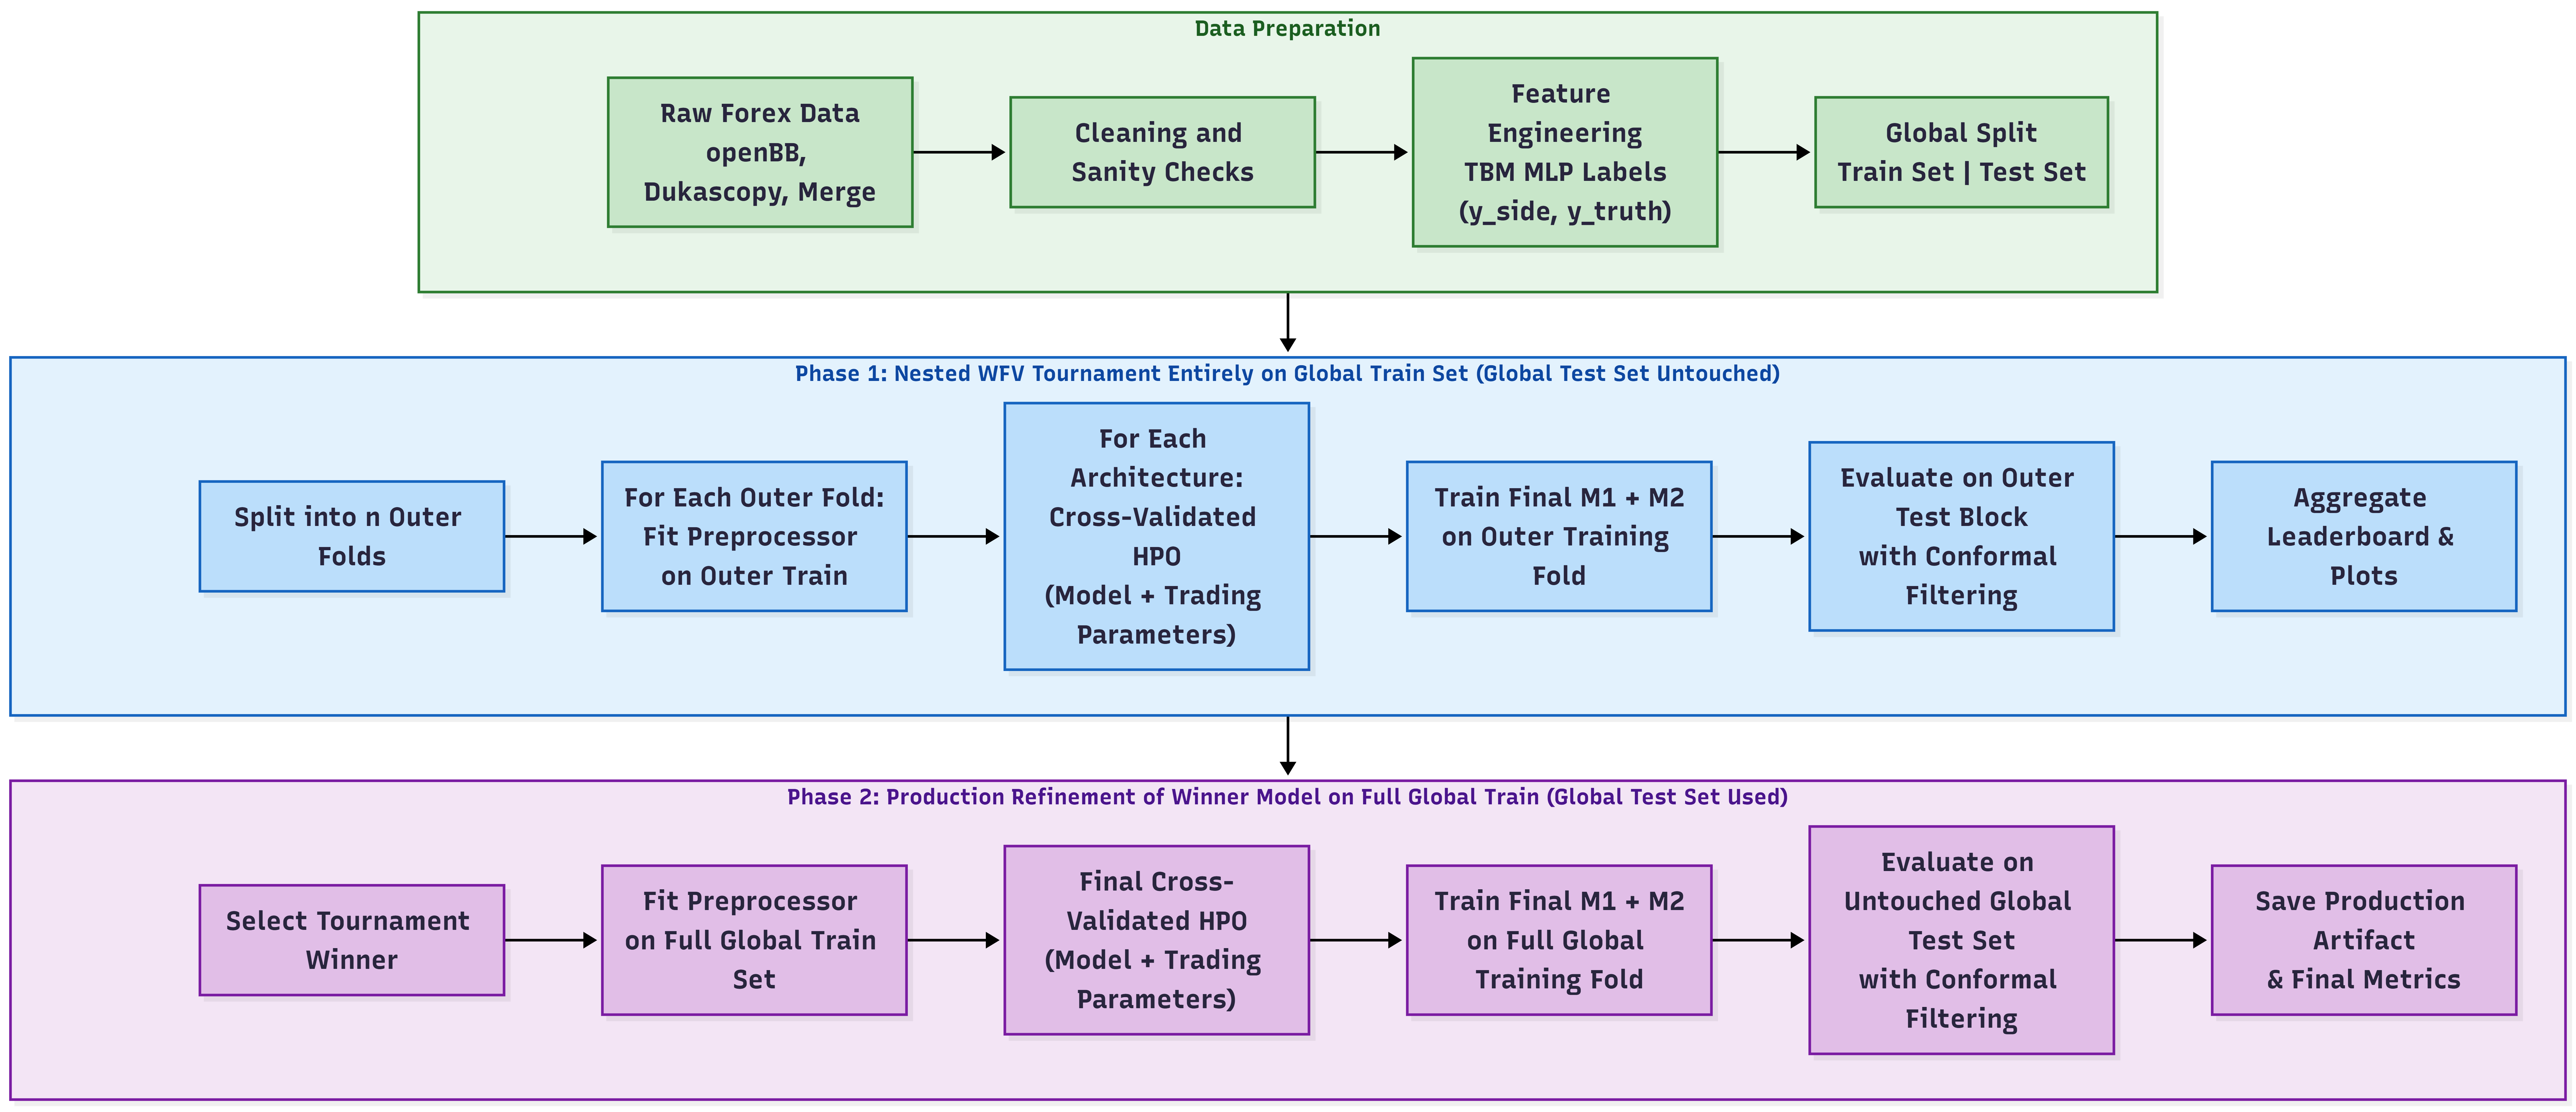
\includegraphics[width=1\linewidth]{../data/figures/methodology/Methodology Flowchart.png}
    \caption{Methodology Overview}
    \label{fig:methodology flowchart}
\end{figure}

\begin{figure}[H]
    \centering
    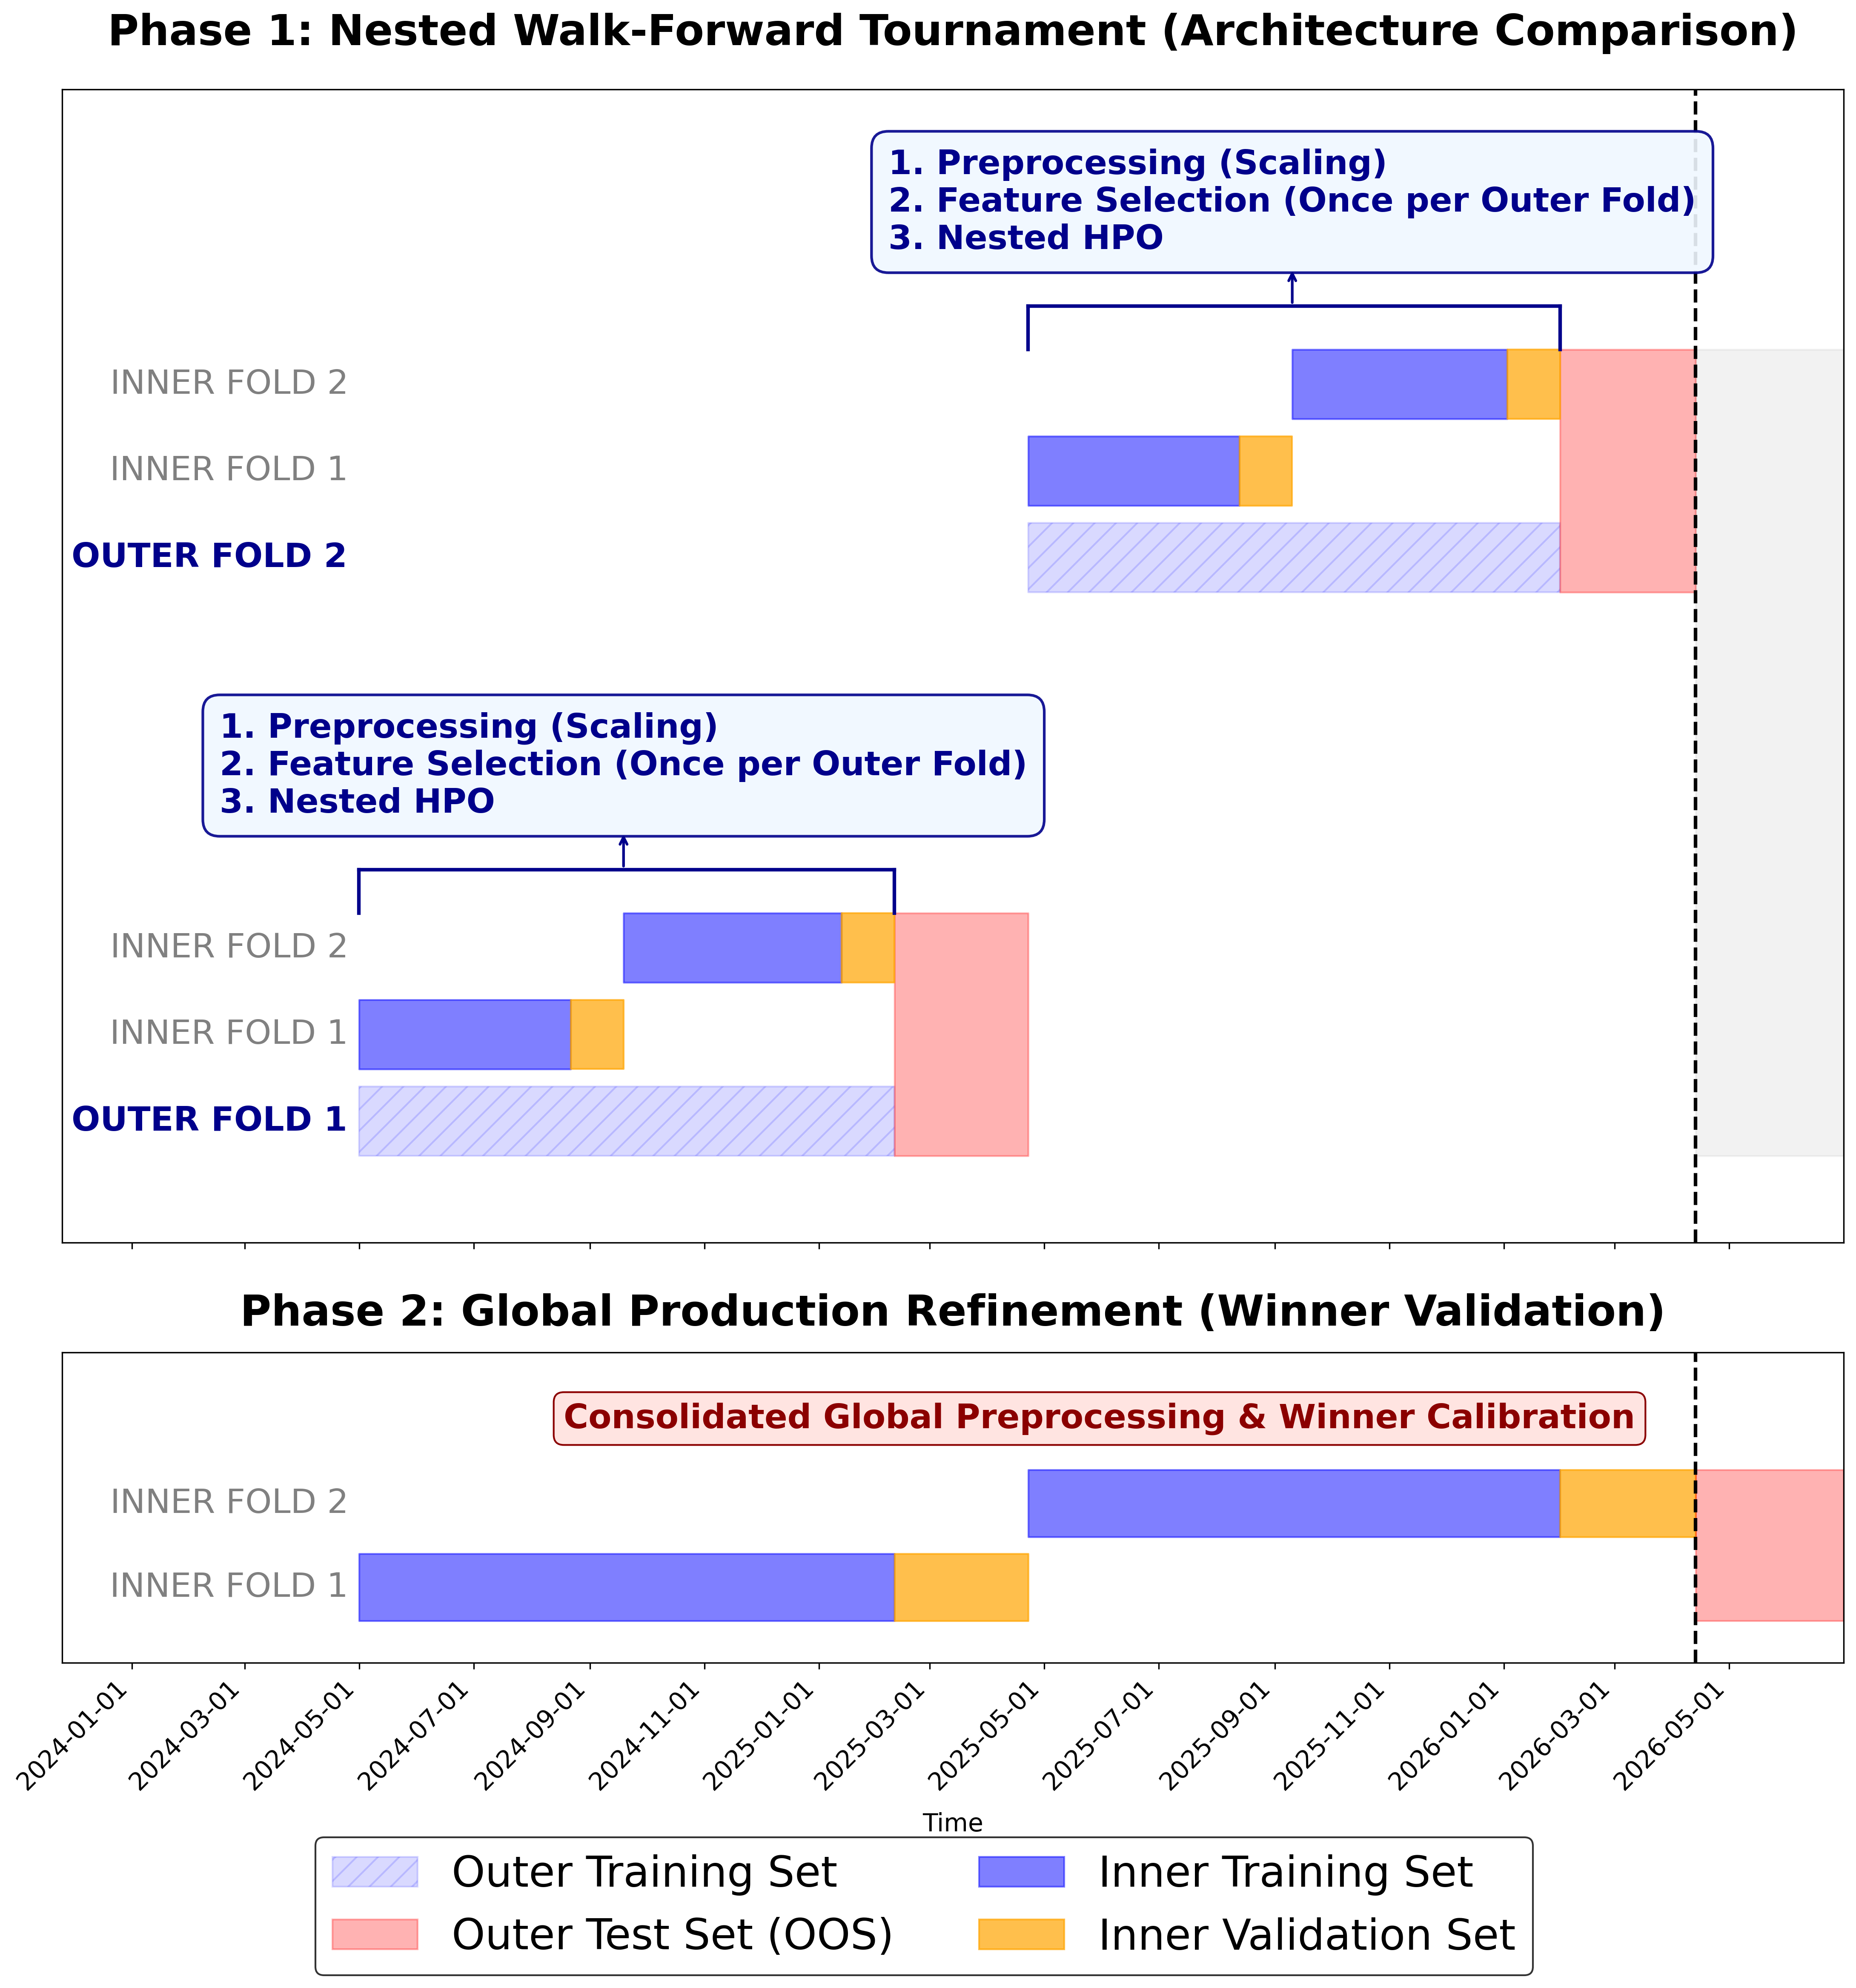
\includegraphics[width=0.6\linewidth]{../data/figures/methodology/pipeline_structure.png}
    \caption{Timeseries Split of the Tournament and Production Pipeline}
    \label{fig:pipeline structure}
\end{figure}


\subsection{Data Preparation}

\subsubsection{Multi-Pair Data Acquisition}\label{sec:data_acquisition}

The data acquisition process is designed to consolidate two different sources into a unified historical dataset.
Hourly OHLCV data is retrieved via the OpenBB SDK, utilizing the Polygon.io provider. 
The system iterates over a list of Forex pairs and performs for each pair incremental updates by detecting the the last timestamp in the local CSV. 
It then tries to fetch as much data as possible in a single API request starting from the last timestamp while respecting a "backoff" period that accounts for the 
number of fetching attempts and API rate limits. If there is no last timestamp, i.e. data is requested for the very first time, the first timestamp will be placed roughly two years 
in the past as this is the maximum period available within the free tier of the polygon API. However, the code allows to extend the dataset every additional day the
script runs, thus, this research has more than two years worth of data available.
Additionally, hourly bid and ask candles are requested from Dukascopy's datafeed which are delivered as compressed binary .bi5 (LZMA) files. 
The module decodes these binary files, unpacking raw integer values (Time, Open, Close, Low, High, Volume) into human-readable prices.
In the final stage both data sources are merged into a single dataset for each specific pair. A critical technical challenge in this phase is the 
synchronization of timestamps as Dukascopy data arrives in Unix time (milliseconds since epoch) and OpenBB arrives in datetime. 
The system enforces a merge by coordinating both sources to the UTC+0 timezone and discards duplicate rows that were generated by the incremental API requests. 
The resulting file provides a holistic view of each hourly bar, containing transaction prices alongside the exact bid/ask spreads available at that time.


\subsubsection{Sanity Checks}\label{sec:sanity_checks}

The raw consolidated dataset undergoes multiple steps to ensure that the machine learning models are trained on valid, tradeable market data. However, the cleaning
process prioritizes market logic over purely statistical filtering which is why the majority of actions taken relate to sanity checks.
Firstly, we scan for bars that are impossible to have occured during live market hours and are more than anything an error. 
A bar is flagged and removed if fundamental OHLCV logic is violated (i.e., if the High price is lower than the Low price). 
Additionally, any bars with zero or negative prices, or non-positive volume, are discarded as technical artifacts.
Secondly, timestamps are validated for strict monotonicity and any non-chronological entries are sorted.
Finally, a sophisticated diagnostic is performed to compare transaction prices against the corresponding bid/ask spread. 
While transaction prices should ideally reside within the quoted range, the system analyzes the magnitude of violations using both zero-tolerance and slippage-buffered thresholds. 
It is important to note that these flagged bars are not filtered out during the cleaning phase because the available bid/ask data represents 
the Top-of-Book (Level 1), which only reflects the best quote for standard volume sizes. 
In reality, larger transaction volumes often sweep through the order book, executing at deeper level prices outside the initial spread. 
By retaining these bars, the methodology ensures the dataset remains representative of actual market execution.


\subsubsection{Feature Engineering and Labeling}\label{sec:features_labels}

The scope of the feature engineering process is intentionally delimited to endogenous market variables, a decision that was driven by the significant 
architectural requirements needed to implement a holistic, end-to-end research pipeline in an individual development effort. 
Consequently, expansion of the feature set into exogenous macroeconomic domains was considered outside the current research horizon.
Nevertheless, the feature engineering phase transforms the previously sanitized dataset into a high-dimensional feature space designed to capture momentum, volatility, and market microstructure. 
To facilitate downstream preprocessing, a naming convention is enforced using the prefixes num\_ (numerical), bin\_ (binary), cyc\_ (cyclical), ord\_ (ordinal) and cat\_ (categorical) such that it becomes 
trivial to assign the correct scaler to the respective feature.

\medskip

In order to capture global trading hours, the system encodes time using both binary flags and cyclical transforms.
It does so via binary indicators that identify among others the London, New York, and Asia sessions, as well as overlaps (i.e., London-NY).
Features such as Time-of-day and day-of-week are transformed using sine and cosine functions to cyclical features which ensures that the 
model perceives the circular nature of time (i.e., that hour 23 is close to hour 0).
To move beyond raw price data, a broad range of technical and momentum indicators is engineered to quantify price velocity, trend exhaustion, and prevailing market regimes. 
This category focuses on capturing the "energy" and stability of price movements, providing the model with normalized signals that distinguish between 
low-volatility ranging markets and high-momentum breakouts across varying look-back windows.
The pipeline leverages bid/ask and volume data to model microstructural dynamics of the market by extracting features related to order flow imbalance, spread fluctuations, and quote
resilience. These microstructural signals try to serve as a proxy for the information content of the order book, offering a deeper view of market state
than traditional price action alone.
Recognizing that market behavior is highly dependent on the active trading session (i.e. London vs. NY), 
interaction features are created to capture the relationship between time-based sessions and price dynamics.
Furthermore, the cat\_pair\_group feature (i.e., Major vs. Emerging Market) was introduced to provide the global model with generizable market context 
without explicitly disclosing the identity of the specific currency pair. 
This abstraction is a deliberate architectural choice to prevent the model from over-fitting to the idiosyncratic historical noise of a single pair, 
while still acknowledging the fundamental differences in volatility and spread profiles between major and exotic instruments.

\medskip

To bridge the gap between feature engineering and supervised learning, the system employs the Triple-Barrier Method introduced by \textcite{lopez_de_prado_advances_2018} and discussed in \ref{sec:label_filter_validate}.

\begin{table}[h]
\centering
\caption{Distribution of Triple-Barrier Labels (Aggregated Dataset)}
\label{tab:label_dist}
\begin{tabular}{lrl}
\toprule
Label & Count & Percentage \\
\midrule
Short & 77023 & 52.65\% \\
Long & 69224 & 47.32\% \\
Timeout & 55 & 0.04\% \\
Total & 146302 & 100.00\% \\
\bottomrule
\end{tabular}
\end{table}


As shown in Table \ref{tab:label_dist}, the resulting dataset exhibits a well-balanced distribution between directional labels. 
It should be noted that while the TBM logic is configured to force a binary (Long/Short) directional classification at the holding period's expiration, 
a negligible number of 55 "Timeout" labels (0.04\%) persist in the aggregated statistics. These represent edge cases at the extreme end of the historical dataset where the
remaining price history was shorter than the required \( t_{\text{final}} \) window, preventing the path-search algorithm from reaching either a price barrier or the full timeout duration.
\footnote{I.e. \( t_{\text{final}} = 5 \) with 11 pairs corresponds to 5 missing labels per pair and 55 missing labels in total.}
These instances are systematically purged during the data alignment phase to ensure that only samples with complete ground-truth outcomes are presented to the models.


\subsection{Strategy Development}

The following methodology details the strategy development within the architectural tournament phase but omits the subsequent production phase as it follows an identical logic.


\subsubsection{Tournament Models}\label{sec:tournament_models}

The tournament phase evaluates a heterogeneous ensemble of machine learning architectures, spanning from classical ensemble methods to modern deep learning structures, 
to identify the most robust learner for high-frequency forex signals. The primary models (M1) include:

\begin{itemize}
    \item Bagging Ensembles (Random Forest \& ExtraTrees): These models operate on the principle of "bootstrap aggregating." They build a large number of independent decision trees 
    on random subsets of the data and average their predictions. This process reduces the risk of the model reacting to random market noise and 
    ensures a more stable prediction by leveraging the "wisdom of the crowd."

    \item Gradient Boosting Decision Trees (XGBoost \& LightGBM): Unlike bagging, boosting models build trees sequentially, where each new tree specifically focuses on 
    correcting the errors made by the previous ones. XGBoost is highly regarded for its precision and regularization techniques that prevent overfitting, 
    while LightGBM is optimized for speed and efficiency, making it particularly effective at processing the large, high-dimensional feature sets common in forex trading.

    \item Recurrent Neural Networks (LSTM \& GRU): These architectures are designed specifically for time-series data. Long Short-Term Memory (LSTM) networks use a "gating" mechanism 
    to selectively remember or forget information over long periods, allowing them to capture deep historical patterns in price action. The Gated Recurrent Unit (GRU) is a more 
    streamlined version of this logic that often achieves similar performance with less computational complexity, providing a faster alternative for sequential learning.
\end{itemize}


\subsubsection{Feature Preprocessing and Selection}\label{sec:preprocessing_scaling}

As already announced in Figures \ref{fig:methodology flowchart} and \ref{fig:pipeline structure} the feature selection and preprocessing logic is executed exactly once per outer training fold.
This obviously leads to a sort of minor lookahead bias in the inner validation sets since a preprocessor that is fitted on the entire outer training fold will transform the data used for 
validation in a way that would be inaccessible for the model during live trading. However, it is of utmost importance to us to note that this lookahead solely occurs on these inner validation 
set (included in the outer training set) and that no data was leaked to the outer testing sets as the preprocessor was never fitted on that data. Furthermore, we selected features from the 
entire available feature space also only once per outer fold for two major reasons. Firstly, it is computationally more efficient to run the selection pipeline once per outer fold as methods 
such as selection via permutation importance can take quite some time depending on the chosen parameters. Secondly, as already mentioned we are not leaking anything to the outer test set.

\medskip

The preprocessing process is fairly lean thanks to the naming convention introduced in \ref{sec:features_labels} which allows granular control over which preprocessor to assign to which group 
of features. Thus, the preprocessor is a singular scikit-learn ColumnTransformer object that uses on the other hand a make\_column\_selector object which selects the respective feature via 
regex patterns. Ultimately, numerical features get assigned a StandardScaler, ordinal features get assigned an OrdinalEncoder, categorical features get assigned a OneHotEncoder, and all others 
are simply let through. Features which do not adhere to the naming convention are discarded for numerical safety.

\medskip

The feature selection process, rather a small pipeline itself, executes a sequential three-step logic to reduce the original feature space based on different filtering methods.
First features are checked for collinearity and highly correlated ones, with an absolute Pearson correlation coefficient exceeding 0.90, are discarded. Next, the remaining features are filtered 
by their mutual information which quantifies the statistical dependency between a feature and the target label measured in their shared entropy. This allows to capture complex non-linear 
relationships that traditional linear correlation metrics may overlook. Finally, features that survived to this point are passed to a permutation importance filter which 
evaluates a feature's predictive utility by measuring the degradation in model performance when that feature's values are randomly shuffled.

\medskip

This hierarchical approach ensures that the resulting feature set is found efficiently and is homogenous among all tournament models.


\subsubsection{The M1-M2 Interaction to Generate Meta-Labels}\label{sec:meta_label_accumulation}

Before the system can generate the meta-labels for the M2 model, M1 has to make predictions (see \ref{sec:label_filter_validate}). 
The labels for M2 are generated by evaluating the performance of the primary M1 model on data it has never seen. For every signal generated by M1 on an inner validation fold, 
the system compares the predicted directional side to the actual triple-barrier label at that time. If M1's directional bet matches the barrier realization, 
the meta-label is assigned a value of 1 for success, otherwise, it is assigned 0 for failure. This allows M2 to specifically learn the behavioral weaknesses and 
mistake patterns of the M1 architecture. In the current implementation M2 is operationalized using a RandomForest Classifier with minimal parameters.
In order to accumulate the labels for M2 across inner folds while ensuring that M2 is not trained and doesn't make predictions on the same set of data, the training of M2 is 
conducted iteratively across the inner folds. On the first inner fold M1 is trained and generates signals, but M2 remains idle as no historical data yet exists for this specific training block.
In subsequent folds before M2 makes a prediction for the current fold, it is trained on the accumulated buffer of all features and meta-labels generated in prior folds. 
This ensures that when M2 evaluates an M1 signal, it is doing so using a model that has never seen the current validation data, maintaining strict temporal separation.
Once the inner walk-forward loop has completed the hyperparameter optimization, a final M2 model is trained on the entire accumulated dataset of the outer block. 
The final M1 and M2 models are then passed to evaluate their performance on truly unseen data on the outer test block in order to provide an unbiased estimate of the 
strategy's production-grade performance. As it would be quite wasteful to discard the historical M2 labels that accumulate across outer folds , a global memory is integrated by 
which the M2 training set is further expanded with a sliding window of historical performance data from previous outer blocks. 
This memory mitigates the problem that in early folds there exists no historical data and provides M2 with a larger, more robust statistical sample of M1's behavior.


\subsubsection{Optimizing Model Architecture and Risk Management Hyperparameters}\label{sec:optimize}

The optimization of the trading system is conducted through a Nested Hyperparameter Optimization (HPO) framework where the outer loop tunes the architectural hyperparameters of the M1 and M2 
models and the inner loop tunes the trading specific hyperparameters. In the outer loop the engine searches for the optimal structural parameters for both the primary model (M1) 
and the meta-filter (M2). For every trial, the system executes a full walk-forward accumulation as discussed in \ref{sec:meta_label_accumulation} to generate statistically unbiased 
out-of-sample (OOS) signals and confidence scores for conformal filtering (see \ref{sec:conformal_preds}). For every architectural candidate proposed by the outer loop, 
a second optimization study is launched in the inner loop which tunes the risk management parameters. These parameters include among others ATR-based stop-loss and take-profit multipliers, 
the fraction applied to the kelly formula, and the conformal significance level applied to the conformal prediction logic.
The objective function maximizes the average Sharpe ratio across the cross-section of currency pairs, ensuring that the winning configuration is robust to diverse market behaviors 
rather than overfitted to a single instrument. To mitigate the "multiple testing" problem inherent in such an exhaustive search, the engine records the variance and total number of 
trials to compute the deflated Sharpe ratio, providing a statistically corrected measure of performance.

\medskip

\textcite{lopez_de_prado_advances_2018} suggests a specific division of labor for meta-labeling wherein the primary M1 model should be configured for high recall, 
acting as a wide net to identify as many potential opportunities as possible, while the secondary M2 model acts as a precision filter to remove false positives. 
In this paradigm, M1 is often a simpler, "looser" rule-set, while M2 is the complex machine that does the "heavy lifting". Our methodology adopts a more integrated approach. 
Rather than fixing M1 as a high-recall "pre-filter", we perform the joint architectural optimization as elaborated above in order to allow the HPO engine to find the global 
optimum where M1 and M2 are most synergistic. By optimizing them together, we ensure that M1 acts as a "stable signal generator" whose errors are not random flukes, but
are statistically significant events that the meta-model is architecturally equipped to recognize and filter.


\subsubsection{Custom Backtester}\label{sec:custom_backtester}

This engine uses Mark-to-Market (MTM) accounting as it updates the account's equity at every single time step, including "floating PnL" from open positions and strictly 
deducts transaction costs (commissions) and slippage (price degradation) at both entry and exit to ensure results are more realistic. 
The core logic of the backtester monitors the distinct exit conditions for every trade whereby it prefers the stop-loss over the take-profit 
even if the take-profit was triggered in the same candle.\footnote{i.e. within the same hourly bar the current high was greater or equal than the take-profit of a long 
but at the same time the current low fell below the stop-loss barrier of the same long, we would record a loss in that case.}
Furthermore, a trade may also be automatically closed after a maximum holding time that was optimized (see \ref{sec:optimize}) or if the underlying model generates a signal in the opposite direction.
It is also crucial to mention the limitation of the engine, as it simplifies the complexities of multi-asset margin management and thus treats each currency pair as an isolated portfolio. It
also enforces a single-position-at-a-time constraint, meaning that no new trades are initiated while a position is already active for a given pair. This approach prioritizes
the granular performance of the strategy on an asset-by-asset basis, effectively omitting cross-pair risk management or global capital allocation strategies in favor of a
more transparent, independent evaluation of each currency pair.

\medskip

The calculation of position size within this framework follows a structured transition from classical gambling theory to modern financial risk management. The foundation
of this approach is the Kelly Criterion \parencite[see][920]{Kelly1956}, which defines the optimal fraction \( \ell \) of capital to bet on an outcome to maximize the
exponential growth of wealth:

\begin{equation}
    \begin{cases}
        (1 + \ell) = 2q \\[4pt]
        (1 - \ell) = 2p
    \end{cases}
    \quad\Longrightarrow\quad
    \ell = q - p
\end{equation}

where \( \ell \) is the fraction of the gambler's current capital to bet, \( p \) is the probability of success, and \( q \) is the probability of failure. 
This framework was later refined and popularized for general investment and gambling scenarios by \textcite[129]{thorp1984mathematics}, 
who introduced the general formula for arbitrary payout ratios:

\begin{equation}
    f^* = \frac{e}{A} = \frac{(A + 1)p - 1}{A}
    \;\Longrightarrow\;
    \boxed{f^* = \frac{bp - q}{b}}
    \qquad\text{where } A = b,\; q = 1-p
\end{equation}

In this formulation, \( f^* \) represents the optimal fraction of capital to bet, \( b \) (or \( A \)) denotes the payout ratio or net odds (net profit per unit risked), 
\( p \) is the probability of success, and \( q \) is the probability of failure. The term \( e = bp - q \) represents the mathematical "edge" or expected value of the bet.

As noted by \textcite[see][p. 876]{macLean2006capital} in \textcite{ziemba2007russell}, betting at or above the log-optimal (Kelly) fraction increases risk. 
This suggests that the aggressive nature of the full Kelly Criterion may lead to excessive volatility and significant drawdowns, 
which could be exceptionally negative in high-noise environments like forex trading.
While the Kelly Criterion provides the idea of conviction-based scaling, the foundational unit of each trade is defined by a risk-parity framework.
Thus, the backtesting engine also adopts the percent risk model introduced by \textcite[292f]{tharp1998trade}. Consequently, the bet in this system is not the total notional value of the portfolio, 
but rather rather a function of equity, risk tolerance, and stop-loss distance, expressed as:

\begin{equation}
    \text{u} = \frac{\text{E} \times \text{R}}{\text{SL}}
    \label{eq:pct_risk_model}
\end{equation}

where \(u\) represents the base position size, \(E\) is the current account capital, \(R\) is the fixed percentage of equity risked per trade, and \(SL\) is the initial stop-loss distance. 
This base size ensures that a stop-loss event results in a loss of exactly \(R\%\) of the portfolio, assuming the signal is valid. To quantify the likelihood of that validity, 
we compute a conformal confidence score \(c\) for each prediction using the calibration framework introduced by \textcite{shafer_tutorial_2008} and defined in Equation \ref{eq:conformal_p}. 
To prevent over-aggressive capital allocation on marginal signals, we transform the conformal excess confidence into a dynamic conviction multiplier using the 
Cumulative Distribution Function (CDF) of the standard Normal distribution, adapting the framework proposed by \textcite[143]{lopez_de_prado_advances_2018}. 
By mapping the confidence score c into a normalized Z-score, the betting size follows a sigmoid curve. This ensures the strategy remains conservative near the significance threshold 
while dynamically scaling towards full risk as statistical conviction increases, effectively penalizing "noisy" predictions in the vicinity of the decision boundary.

\begin{equation}
    \text{z} = \left( \frac{c - (1 - \varepsilon)}{\varepsilon} \right)
\end{equation}

\begin{equation}
    \text{size} = \max\left(0, 2 \times \varPhi(\text{3z}) - 1 \right)
    \label{eq:conviction_mult}
\end{equation}

In this formulation, \( \varepsilon \) represents the tuned significance level (see \ref{sec:optimize}), which serves two critical functions. 
First, the term \( (1 - \varepsilon) \) acts as a statistical floor whereby any prediction with a confidence score c that fails to meet this threshold results in 
\( \text{z} \leq 0 \), which the \( \max\left(0, ...\right) \) operator translates into a size of zero, effectively vetoing the trade. 
Second, \( \varepsilon \) serves as the scaling denominator that normalizes the excess confidence. 
To enable the strategy to reach full conviction (i.e., \( \text{size} \approx 1 \)), we introduce a scaling multiplier of 3 to the normalized Z-score calculation. 
This choice ensures that the conviction multiplier (size) is permitted to traverse the full curvature of the Gaussian CDF, reaching a maximum value of approximately 0.997 
only as the model reaches absolute statistical certainty (\( c = 1.0 \)), which represents the 99.7\% probability mass characteristic of the three-sigma rule.
It is important to distinguish this from the classical Z-score used by \textcite[143]{lopez_de_prado_advances_2018}, which normalizes probabilities by 
\( \text{z} = \frac{\text{p}\left[x=1\right] - \frac{1}{2}}{\sqrt{\text{p}\left[x=1\right] \left(1 - \text{p}\left[x=1\right]\right)}} \) with labels \( x \in \left\{-1,1\right\} \) to test 
\( H_0 : \text{p}\left[x=1\right] = \frac{1}{2} \). In this research, we substitute the \( \sigma \) with the significance level \( \varepsilon \) since the execution logic only 
considers trades where \( c > (1 - \varepsilon) \), the value of \( \varepsilon \) represents the total width of the discovery region \( (1-\varepsilon, 1.0] \). 
Utilizing \( \varepsilon \) as the denominator ensures that the Z-score represents the relative position of the current confidence within this allowed margin. 
This ensures $z=0$ at the threshold and $z=1$ at perfect model certainty, providing a stable and bounded input for the sigmoid transformation.
Ultimately, the final bet size is derived by combining the risk-parity units ( Eq. \ref{eq:pct_risk_model}) with the conviction multiplier (Eq. \ref{eq:conviction_mult}), and 
a tuned Kelly fraction:

\begin{equation}
    \text{Bet} = \text{u} \times \text{size} \times \text{fraction}
    \label{eq:bet}
\end{equation}

This interaction ensures that capital allocation is not only adjusted for price volatility via the stop-loss distance but is also non-linearly scaled by the strength of the 
statistical evidence provided by the conformal engine.


\subsubsection{Evaluation on OOS Test Data}\label{sec:oos_evaluation}

The final stage of the Nested Walk-Forward Validation (WFV) architecture is the unbiased evaluation of the optimized pipeline on the isolated outer test block. 
This phase serves as the definitive assessment of the strategy's robustness, simulating a "live" deployment where the model encounters entirely unseen market regimes.
To maintain strict out-of-sample (OOS) integrity, the evaluation begins with the application of the preprocessing logic established in \ref{sec:preprocessing_scaling}. 
Specifically, the test data is transformed using the singular ColumnTransformer that was fitted exclusively on the corresponding outer training fold. 
Similarly, the feature set is restricted to those identified by the hierarchical selection pipeline in \ref{sec:preprocessing_scaling}, ensuring that the architectural tournament 
is conducted on a consistent and pruned informational subset.
The predictive execution follows a dual-model flow where the primary model (M1) generates directional signals, while the secondary model (M2) provides the raw probability of M1's success. 
As established in \ref{sec:meta_label_accumulation}, these raw probabilities are not utilized directly but are instead passed through a conformal filtering layer. 
The system calculates a dynamic p-value for each prediction by comparing the current M2 probability to the calibration set of historical M1 mistakes accumulated from prior folds. 
If the resulting p-value meets the per-pair significance threshold \( \varepsilon \) optimized in \ref{sec:optimize}, the trade is authorized.
The authorized signals are subsequently processed by the backtesting engine (see \ref{sec:custom_backtester}), which implements the risk-parity and non-linear sigmoid sizing logic 
defined in Equations \ref{eq:pct_risk_model} through \ref{eq:bet}. A distinguishing feature of this evaluation phase is the use of per-pair hyperparameter adaptation. 
Unlike a "one-size-fits-all" approach, the backtester utilizes the unique ATR-based stop-loss, take-profit, and max-holding periods identified during the inner optimization study 
(see \ref{sec:optimize}) for each specific currency pair.

To validate the statistical "value-add" of the conformalized meta-labeling approach, the system benchmarks the resulting performance against five distinct strategies:
\begin{enumerate}
    \item Buy and Hold: A passive benchmark representing the raw beta of the currency pair.
    \item SMA Crossover: A technical baseline using 50/200-period moving average logic.
    \item M1 Only: An evaluation of the primary directional signals with optimized risk guardrails but without the meta-labeling filter.
    \item M1 + M2 (Fixed): A version using the meta-model with a static 0.5 probability threshold, aiming to prove the necessity of the conformal calibration.
    \item M1 + M2 (Global): A baseline utilizing the median hyperparameters across all pairs, which isolates the performance benefit gained from the "local" per-pair adaptation discussed in \ref{sec:optimize}.
    \item M1 + M2 (Conformal): The full proposed pipeline utilizing optimized architectural parameters, per-pair risk hyperparameters, and conformalized conviction-based bet sizing.
\end{enumerate}

Finally, the strategies are subjected to several reported metrics, especially the deflated Sharpe ratio (DSR). By integrating the total number of trials and the variance of Sharpe ratios recorded during 
the HPO phase (see \ref{sec:optimize}), the methodology provides a corrected estimate of performance that accounts for the selection bias inherent in hyperparameter search. 


\subsubsection{Empirical Evaluation Metrics and Diagnostic Framework}\label{sec:empirical_framework}

The final component of the methodology describes the framework through which the tournament models are evaluated. 
To ensure a multi-dimensional assessment of performance, we employ a wide range of financial metrics which can be found among others in section \ref{sec:backtest_overfitting} 
(Eq. \ref{eq:psr} and \ref{eq:sr_star}), and appendix \ref{app:metrics} (Eq. \ref{eq:sharpe_ratio} to \ref{eq:mintrl}).

\medskip

Beyond financial outcomes we ensure the feature selection pipeline (\ref{sec:preprocessing_scaling}) effectively prunes the informational space by utilizing nested correlation heatmaps 
across outer folds to monitor multicollinearity. Furthermore, we conduct a post-mortem analysis of the model's decision-making process using permutation importance scores. 
By tracking the stability of these importance rankings across different outer folds, we hope to distinguish between universal features that provide stable alpha and 
regime-specific features that may indicate temporary over-fitting.

\medskip

To audit the efficacy of the conformal logic, we utilize a conformal signal analysis plot that scatter-maps M2 confidence against signal directions. 
By color-coding these samples based on empirical correctness, we can visualize the separation between valid signals and noise. 
An effective filter demonstrates a high concentration of correct predictions at high confidence levels, while incorrect predictions are concentrated within the conformal rejection
zone defined by $\varepsilon$. Furthermore, we overlay a logistic sigmoid fit to this diagnostic plot to verify that the M2 probability estimates are well-calibrated 
against the true empirical hit rate of the M1 signals.
A logistical limitation of this visualization is its level of aggregation. To be fully exhaustive, an informative diagnostic would require rendering three panels 
(Accuracy, Ground Truth, and Error Map) for every individual model-pair combination across all folds. In a tournament of six architectures and ten currency pairs, this would
generate an unmanageable 60 plot-triplets per fold, totaling hundreds of figures. Consequently, we employ a lighter aggregated version in this study whereby the scatter plots displayed in 
the results aggregate all currency pairs for a given architecture within a specific fold. This provides a global view of the architecture's robustness and its ability to
generalize a conformal veto logic across the entire multi-pair universe without the visual overhead of per-pair reporting.

\medskip

Beyond financial outcomes, the integrity of the meta-labeling engine (M2) is evaluated through classification-specific diagnostics. We utilize confusion matrices to monitor the balance 
between Type I errors (False Discoveries) and Type II errors (Missed Opportunities). To assess the probabilistic quality of the meta-model, we employ reliability diagrams (calibration curves), 
which compare the predicted probabilities of M2 against the actual observed frequencies of M1's correctness. A well-calibrated model, where the curve aligns with the 45-degree diagonal, 
ensures that the conformal p-values calculated in \ref{sec:conformal_preds} are grounded in realistic probability estimates.

The integrity of the meta-labeling engine is further examined through classification-specific diagnostics, primarily utilizing nested confusion matrices and reliability diagrams. 
The three-panel confusion matrix framework tracks signals from the base model (M1) through the meta-model (M2) to the final authorized trades. 
It allows to follow the flow of the balance between Type I errors (False Discoveries) and Type II errors (Missed Opportunities). 
To complement this, reliability diagrams and Brier scores are employed to assess the probabilistic quality of the meta-model. 
By verifying that the calibration curve aligns with the 45-degree diagonal, we ensure that the conformal p-values calculated in \ref{sec:conformal_preds} are grounded in realistic 
probability estimates.

\medskip

\paragraph{LOOK AT THIS AGAIN!}
To identify the ultimate tournament winner, we utilize a reciprocal rank fusion (RRF) and aggregated performance ranking. Models are ranked based on their mean Sharpe Ratio across all 
outer test folds and all currency pairs. This "Global Mean" approach penalizes architectures that perform exceptionally well in a single regime but fail to generalize across the 
diverse liquidity and volatility profiles of the full multi-pair dataset.


%%%%%%%%%%%%%%%%%%%%%
% EMPIRICAL RESULTS %
%%%%%%%%%%%%%%%%%%%%%
\section{Empirical Results}
\subsection{The Architecture Tournament}

This section presents the empirical findings of the Architecture Tournament, representing the first major phase of our experimental validation framework 
(as outlined in Figure \ref{fig:methodology flowchart}). The primary objective of this phase is to conduct an unbiased, out-of-sample peer comparison of the candidate 
model architectures detailed in \ref{sec:tournament_models} across the currency pairs. To prevent the pervasive issue of backtest overfitting discussed in 
\ref{sec:backtest_overfitting}, the tournament is executed within a nested walk-forward validation framework as illustrated in Figure \ref{fig:pipeline structure}. 
The operational pipeline for the tournament proceeds through the following sequential steps:

\begin{itemize}
\item \textbf{Feature Preprocessing}: Before training, the information space is pruned to exclude multicollinear features using the hierarchical selection 
pipeline in \ref{sec:preprocessing_scaling}. This ensures a static, homogeneous feature space across all competing architectures for a given fold.

\item \textbf{Conformal Filtering}: Raw probability predictions from the meta-model \ref{sec:conformal_preds} are mapped to dynamical 
conformal p-values. Signals that fall within the conformal rejection zone defined by the significance level are vetoed.

\item \textbf{Hyperparameter Optimization}: The combined signals are evaluated using the custom backtester (see \ref{sec:custom_backtester}). 
Hyperparameters are optimized to maximize the Sharpe ratio.

\item \textbf{Reciprocal Rank Fusion (RRF)}: The competing models are ranked globally based on their average performance across all outer folds and currency pairs. 
The tournament winner is selected using the aggregated RRF matrix framework described in Section \ref{sec:empirical_framework}.
\end{itemize}

By evaluating the architectures through this multi-layered protocol, we ensure that the top-performing model is not merely a product of regime-specific luck, 
but a robust architecture capable of generating stable, conformalized alpha.


\subsubsection{Static Feature Space Definition Across All Tournament Models (Common Feature Set Per Fold) and Multicollinearity Filtering}

To ensure a fair comparison across the tournament's competing model architectures, feature selection was performed once per outer fold rather than once per model,
yielding a single, common feature set that every M1 candidate in that fold was subsequently trained and evaluated on (see \ref{sec:preprocessing_scaling}). 
As a reminder, the selection proceeds in three sequential stages where first an unsupervised correlation filter removes redundant features irrespective of their 
relationship to the target ($|\rho| > 0.90$), followed by a supervised Mutual Information filter that discards features falling below a minimum 
univariate association with the M1-label ($\text{MI}_{\text{thresh}} < 0.005$), and finally a permutation importance filter, which prunes any remaining feature 
contributing negligible or negative predictive value to a reference model ($\text{PI}_{\text{thresh}} \leq 0.001$).

\medskip

Figure \ref{fig:correlation filtering} (see \ref{app:tourney_feat_select}) shows the correlation matrices of the feature space for both outer folds before and after 
filtering for correlation. In total, the pipeline filtered out 12 features out of 94 in the first outer fold and 11 features in the second outer fold.
The similarity between the Fold 1 and Fold 2 "AFTER" panels also suggests that the correlation structure of the feature space itself is
reasonably stable across the two evaluation windows, even before any target-aware filtering is applied.

\begin{figure}[H]
    \centering
    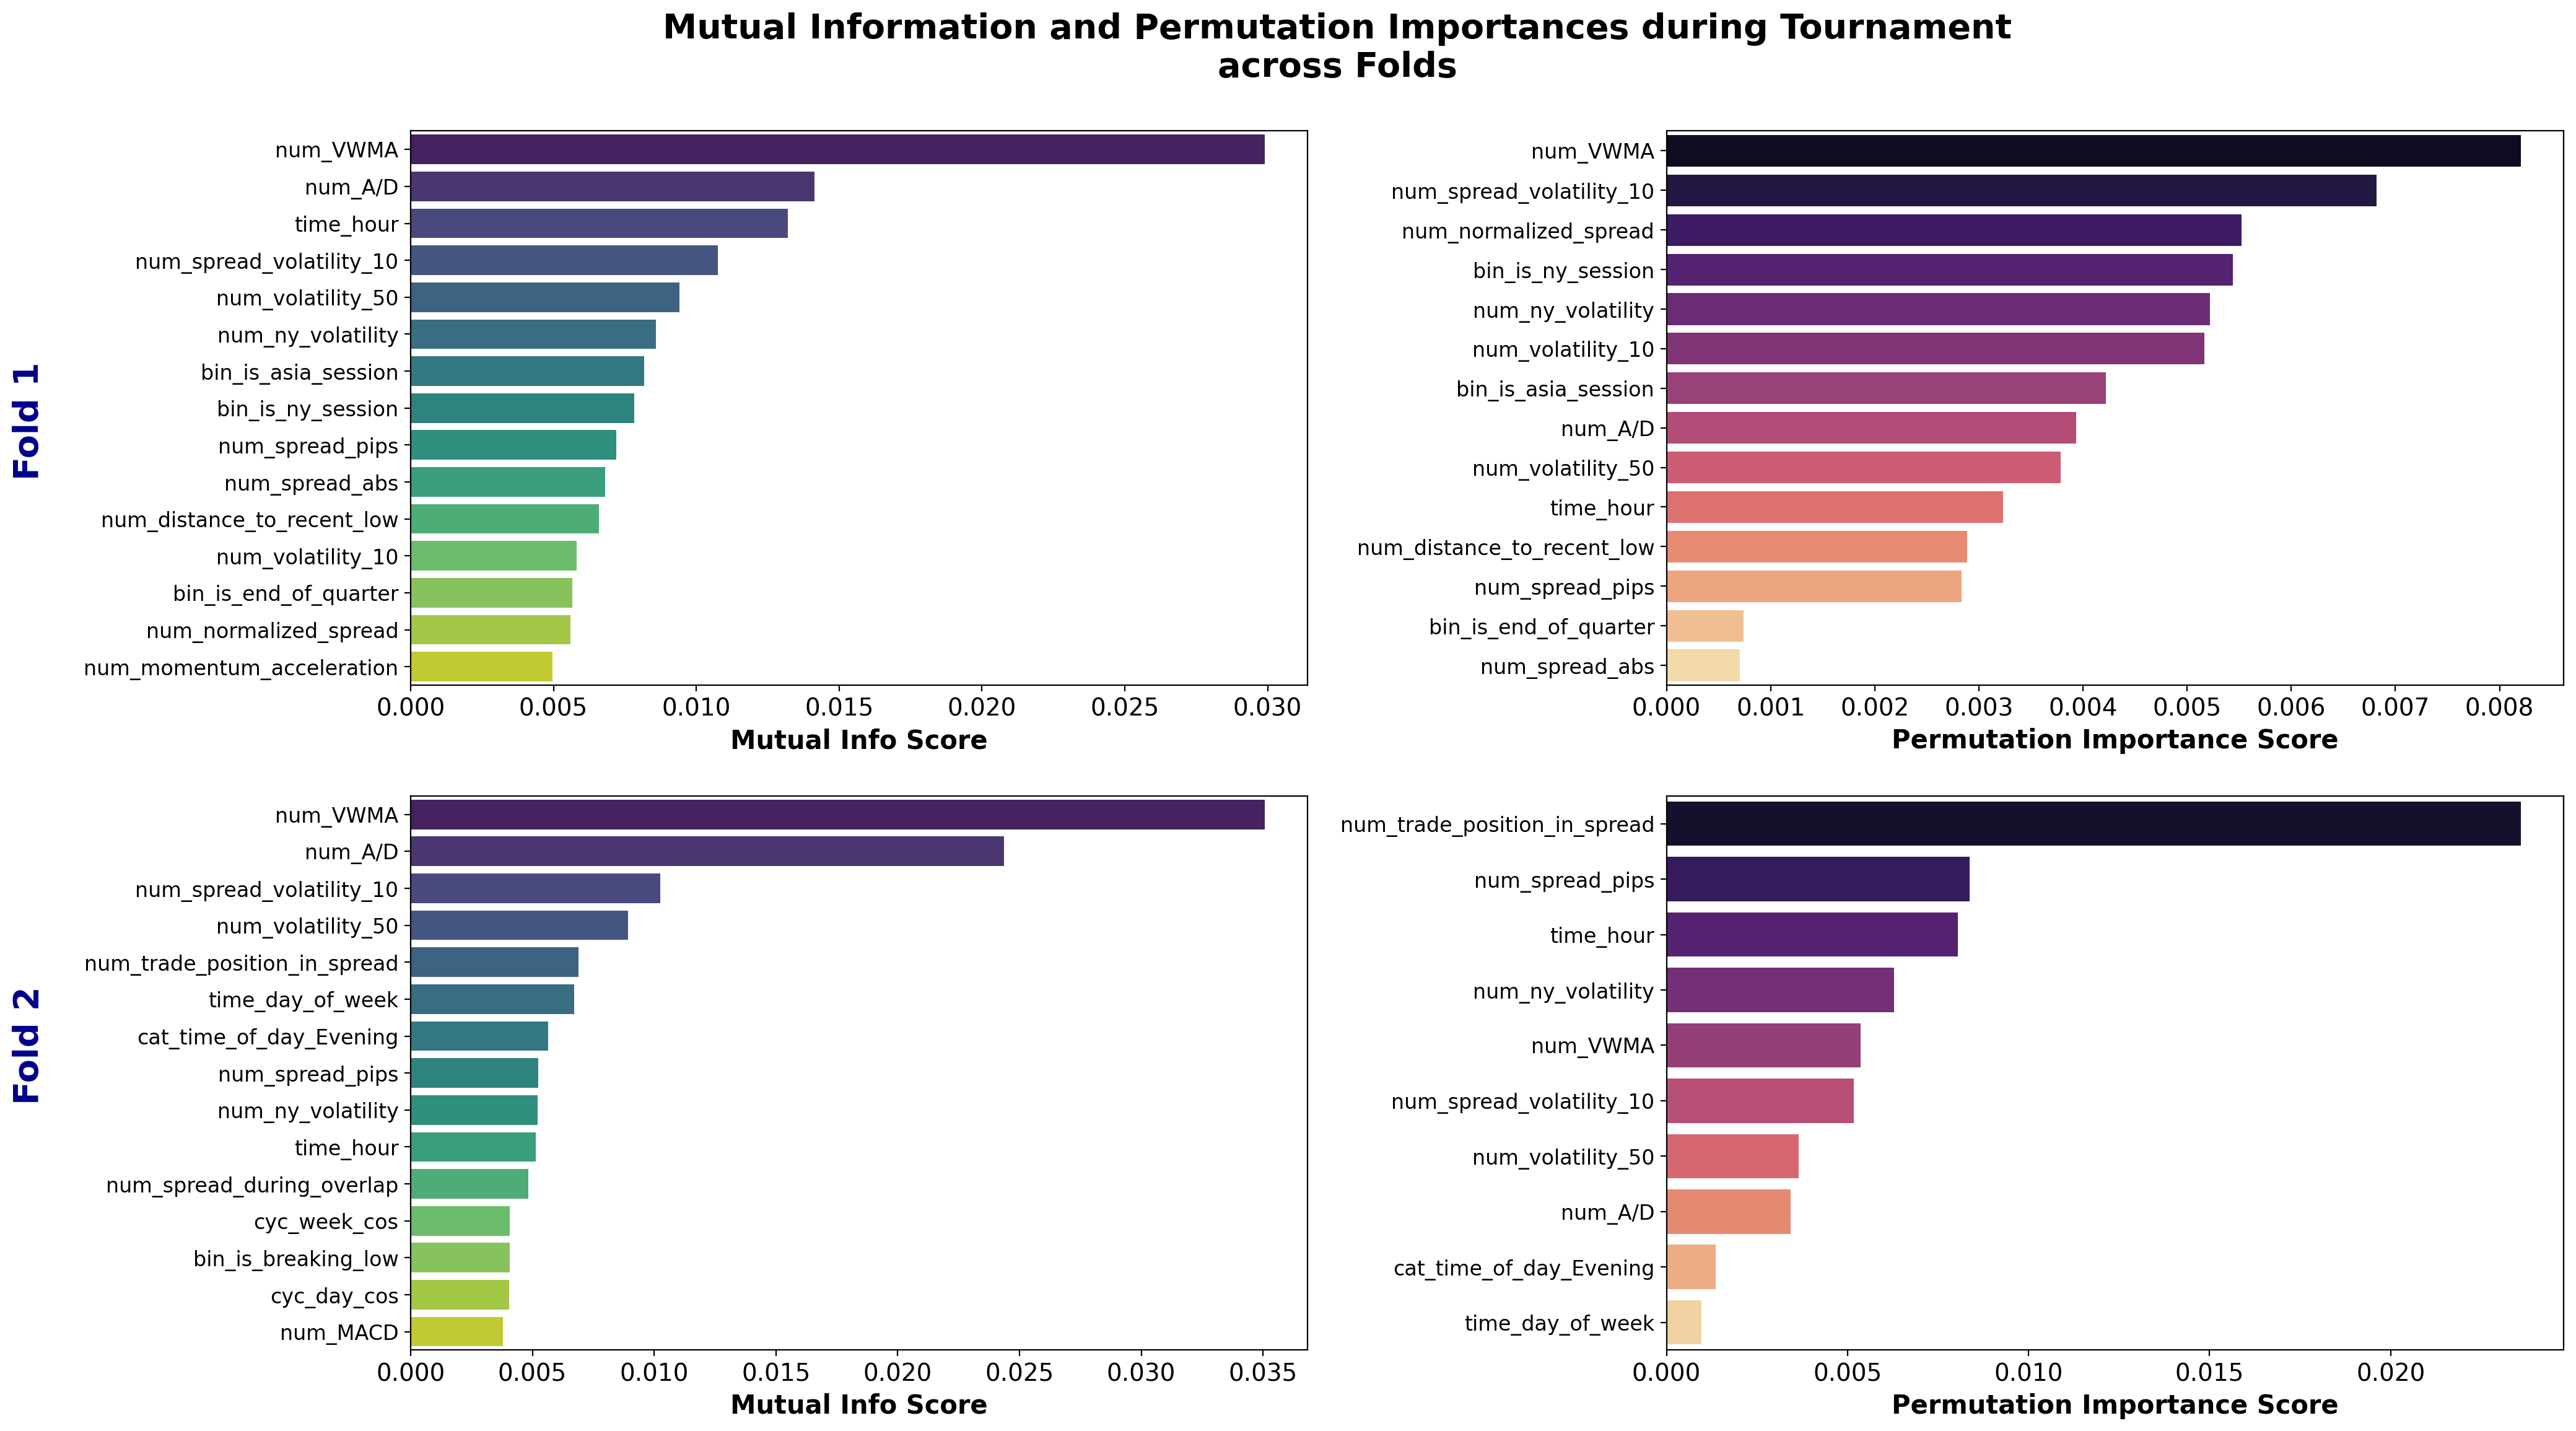
\includegraphics[width=0.95\linewidth]{../data/figures/feature_selection/Tournament_nested_feature_importances_RandomForest.png}
    \caption{Feature Importances During Tournament}
    \label{fig:feature importances}
\end{figure}

Figure \ref{fig:feature importances} then illustrates the two supervised stages applied on top of this pre-filtered set. Two observations stand out: 

\medskip

First, the MI and permutation importance rankings agree only partially: in fold 1, num\_VWMA dominates by a wide margin under both metrics and is still relevant in the second fold. 
Furthermore, num\_A/D, num\_spread\_volatility\_10, num\_volatility\_50, num\_ny\_volatility, and num\_spread\_pips rank consistently on roughly the same positions across both 
folds in the MI score and all of them also remain relevant in the subsequent PI scores across both folds suggesting their structural relevance across time.
However, the remainder of the ranking reshuffles considerably. In both folds of the top features by MI score some features that are included in one fold but not the other are
bin\_is\_asia\_session, bin\_is\_ny\_session, num\_spread\_abs, num\_normalized\_spread to name a few. In PI ranking, features in this category are num\_normalized\_spread, 
bin\_is\_ny\_session, bin\_is\_asia\_session, num\_distance\_to\_recent\_low to name a few again.
Also, it is worth noting that features that rank highly in the MI section might not rank on the same position in the PI score, which is consistent with MI capturing marginal, 
univariate association with the label, while permutation importance reflects a feature's marginal
contribution to the fitted model's predictive performance, including any interaction effects with other retained features. Thus, a feature can be MI-weak yet
model-critical or vice versa precisely because of such interactions. 

\medskip

Second, and more importantly for the "static feature set" motivation of this section, the two folds
themselves disagree substantially on which features matter most. For example, num\_trade\_position\_in\_spread is the single most important feature by permutation importance in
Fold 2, yet it does not even register among the top PI features in Fold 1's ranking. Additionally, the fold-to-fold instability of the features in the PI metric is precisely the 
kind of overfitting risk that motivates selecting a single, common feature set per fold across all tournament models rather than allowing each model architecture to select its own, 
possibly unstable, feature subset, which would confuse genuine architectural differences with differences in feature selection noise.


\subsubsection{Pair- and Model-Specific Parameter Discovery and Financial Robustness}

Having established a common static feature set per fold to mitigate overfitting and ensure comparability across architectures, we now turn to the model-specific hyperparameter 
optimization and its financial implications. While the tournament includes multiple model classes, we focus the present discussion exclusively on the XGBoost results, 
as presenting exhaustive tables and figures for every candidate model would be both space-prohibitive and unnecessarily repetitive. The XGBoost architecture serves as a 
representative gradient-boosted tree model, and its performance during the tournament phase is illustrative of the broader patterns observed across the ensemble of competing methods.
Please find tables and figures regarding the other models in the tournament appendix \ref{app:tournament}.

\begin{table}[H]
\centering
\caption{Hyperparameters for XGBoost Model (Tournament Phase)}
\label{tab:hps_XGBoost_tournament}
\resizebox{\textwidth}{!}{%
\begin{tabular}{lccccccccccc}
\toprule
 & \rot{AUDUSD} & \rot{EURUSD} & \rot{GBPUSD} & \rot{NZDUSD} & \rot{USDCAD} & \rot{USDCHF} & \rot{USDCNH} & \rot{USDJPY} & \rot{USDMXN} & \rot{USDTRY} & \rot{USDZAR} \\
\midrule
\multicolumn{11}{c}{\textbf{Fold 1}} \\
\midrule
Kelly F. & 0.48 & 0.70 & 0.72 & 0.33 & 0.99 & 0.42 & 0.61 & 0.73 & 0.32 & 0.38 & 0.76 \\
MH & 50.00 & 39.00 & 15.00 & 15.00 & 38.00 & 19.00 & 25.00 & 34.00 & 17.00 & 14.00 & 17.00 \\
Max Exp. & 65.00 & 87.00 & 61.00 & 89.00 & 90.00 & 63.00 & 88.00 & 83.00 & 98.00 & 64.00 & 89.00 \\
Meta Sig. & 0.09 & 0.05 & 0.02 & 0.06 & 0.08 & 0.13 & 0.15 & 0.10 & 0.01 & 0.12 & 0.20 \\
Risk Pct. & 0.02 & 0.0098 & 0.01 & 0.02 & 0.0052 & 0.02 & 0.01 & 0.02 & 0.02 & 0.02 & 0.02 \\
SL Mult. & 2.65 & 4.15 & 2.23 & 3.07 & 4.88 & 2.50 & 2.62 & 2.96 & 2.12 & 4.41 & 4.16 \\
TP Mult. & 2.55 & 3.68 & 4.56 & 3.12 & 4.02 & 2.23 & 4.18 & 4.88 & 1.89 & 1.88 & 4.67 \\
\midrule
\multicolumn{11}{c}{\textbf{Fold 2}} \\
\midrule
Kelly F. & 0.71 & 0.33 & 0.22 & 0.83 & 0.29 & 0.64 & 0.47 & 0.56 & 0.28 & 0.49 & 0.30 \\
MH & 6.00 & 14.00 & 15.00 & 18.00 & 37.00 & 25.00 & 10.00 & 27.00 & 37.00 & 50.00 & 27.00 \\
Max Exp. & 65.00 & 90.00 & 86.00 & 67.00 & 86.00 & 91.00 & 50.00 & 73.00 & 60.00 & 91.00 & 84.00 \\
Meta Sig. & 0.10 & 0.16 & 0.08 & 0.10 & 0.09 & 0.04 & 0.03 & 0.17 & 0.17 & 0.01 & 0.06 \\
Risk Pct. & 0.03 & 0.02 & 0.02 & 0.03 & 0.02 & 0.0062 & 0.01 & 0.03 & 0.02 & 0.02 & 0.02 \\
SL Mult. & 5.00 & 4.29 & 2.64 & 3.14 & 1.59 & 2.94 & 1.86 & 3.73 & 1.06 & 3.90 & 3.64 \\
TP Mult. & 3.71 & 3.14 & 2.50 & 4.95 & 2.60 & 4.17 & 2.10 & 3.27 & 1.79 & 2.35 & 1.09 \\
\bottomrule
\end{tabular}
}%
\end{table}

Before turning to these patterns, it is useful to briefly define the seven trading-level hyperparameters reported in table \ref{tab:hps_XGBoost_tournament}, all of which are tuned 
jointly, per pair and per fold, by the same Optuna study. \textbf{Risk Pct.} sets the fraction of current equity that is risked if the stop-loss is hit, and together 
with \textbf{SL Mult.} (the stop-loss distance, expressed as a multiple of ATR) determines the base position size via risk-parity sizing (see eq. \ref{eq:pct_risk_model}). 
\textbf{TP Mult.} sets the take-profit distance analogously, but plays no role in sizing. 
\textbf{Kelly F.} is a fractional multiplier in $[0,1]$ applied on top of this risk-parity base size, throttling it back from full growth-optimal (Kelly-criterion) sizing toward a 
more conservative fraction thereof. \textbf{Meta Sig.} is the significance level of the conformal veto, which sets the confidence threshold the M2 meta-model's calibrated probability 
must clear for a candidate M1 signal to be acted upon at all, with lower values corresponding to a stricter (more selective) filter. \textbf{MH} caps the number of bars a trade is 
permitted to remain open before being forcefully closed irrespective of whether its stop-loss or take-profit has been reached, and is therefore a time-based backstop on trade duration 
rather than a sizing parameter. Finally, \textbf{Max Exp.} is the maximum permissible notional exposure, expressed as a percentage of mark-to-market equity. Unlike the parameters 
above, it does not participate in determining position size at all, but instead acts as a hard ceiling that clips the risk-parity-derived size downward if, and only if, that size 
would otherwise exceed it.

\medskip

\ref{tab:hps_XGBoost_tournament} reports the hyperparameters selected by the trading-level Optuna study for each currency pair and fold. Several patterns are worth highlighting, such as 
the Kelly fraction, which shows substantial cross-sectional heterogeneity within a single fold (e.g. Fold 1 ranges from $0.11$ for USDCNH to $0.94$ for USDMXN), 
indicating that the optimizer does not converge on a single universal position-sizing aggressiveness but instead tries to tailor it to each pair's realized edge and volatility profile. 
Second, the maximum holding period (MH) ceiling is systematically lower in Fold 2 than in Fold 1 for the majority of pairs (e.g. GBPUSD drops from 43 to 11 bars, USDTRY from 33 to 10). 
Since MH only caps how long a trade is permitted to remain open before being forcefully closed and the barrier-based exit logic (stop-loss/take-profit) typically resolves 
trades well before this ceiling is reached, this shift is better read as the optimizer tightening the outer time budget available to trades in Fold 2 rather than as direct evidence 
that realized trade durations themselves become shorter.
Third, the discovered notional exposure ceiling (Max Exp.) clusters toward the upper half of its permissible search range ($50\%$-$100\%$) for most pairs in both folds, 
frequently exceeding $80\%$, however, as we will see below, this ceiling is rarely binding in practice, since realized average exposure sits considerably lower. 
Finally, the stop-loss and take-profit multipliers show no consistent asymmetry across pairs as some pairs favor a wider take-profit relative to stop-loss 
(e.g. USDMXN, Fold 1: SL $3.40\times$ ATR vs. TP $4.79\times$ ATR), while others favor the reverse (e.g. USDZAR, Fold 1: SL $3.56\times$ ATR vs. TP $1.37\times$ ATR), 
suggesting that the profitable risk-reward geometry is itself pair- and regime-specific rather than a fixed, universally superior ratio.

\begin{figure}[H]
    \centering
    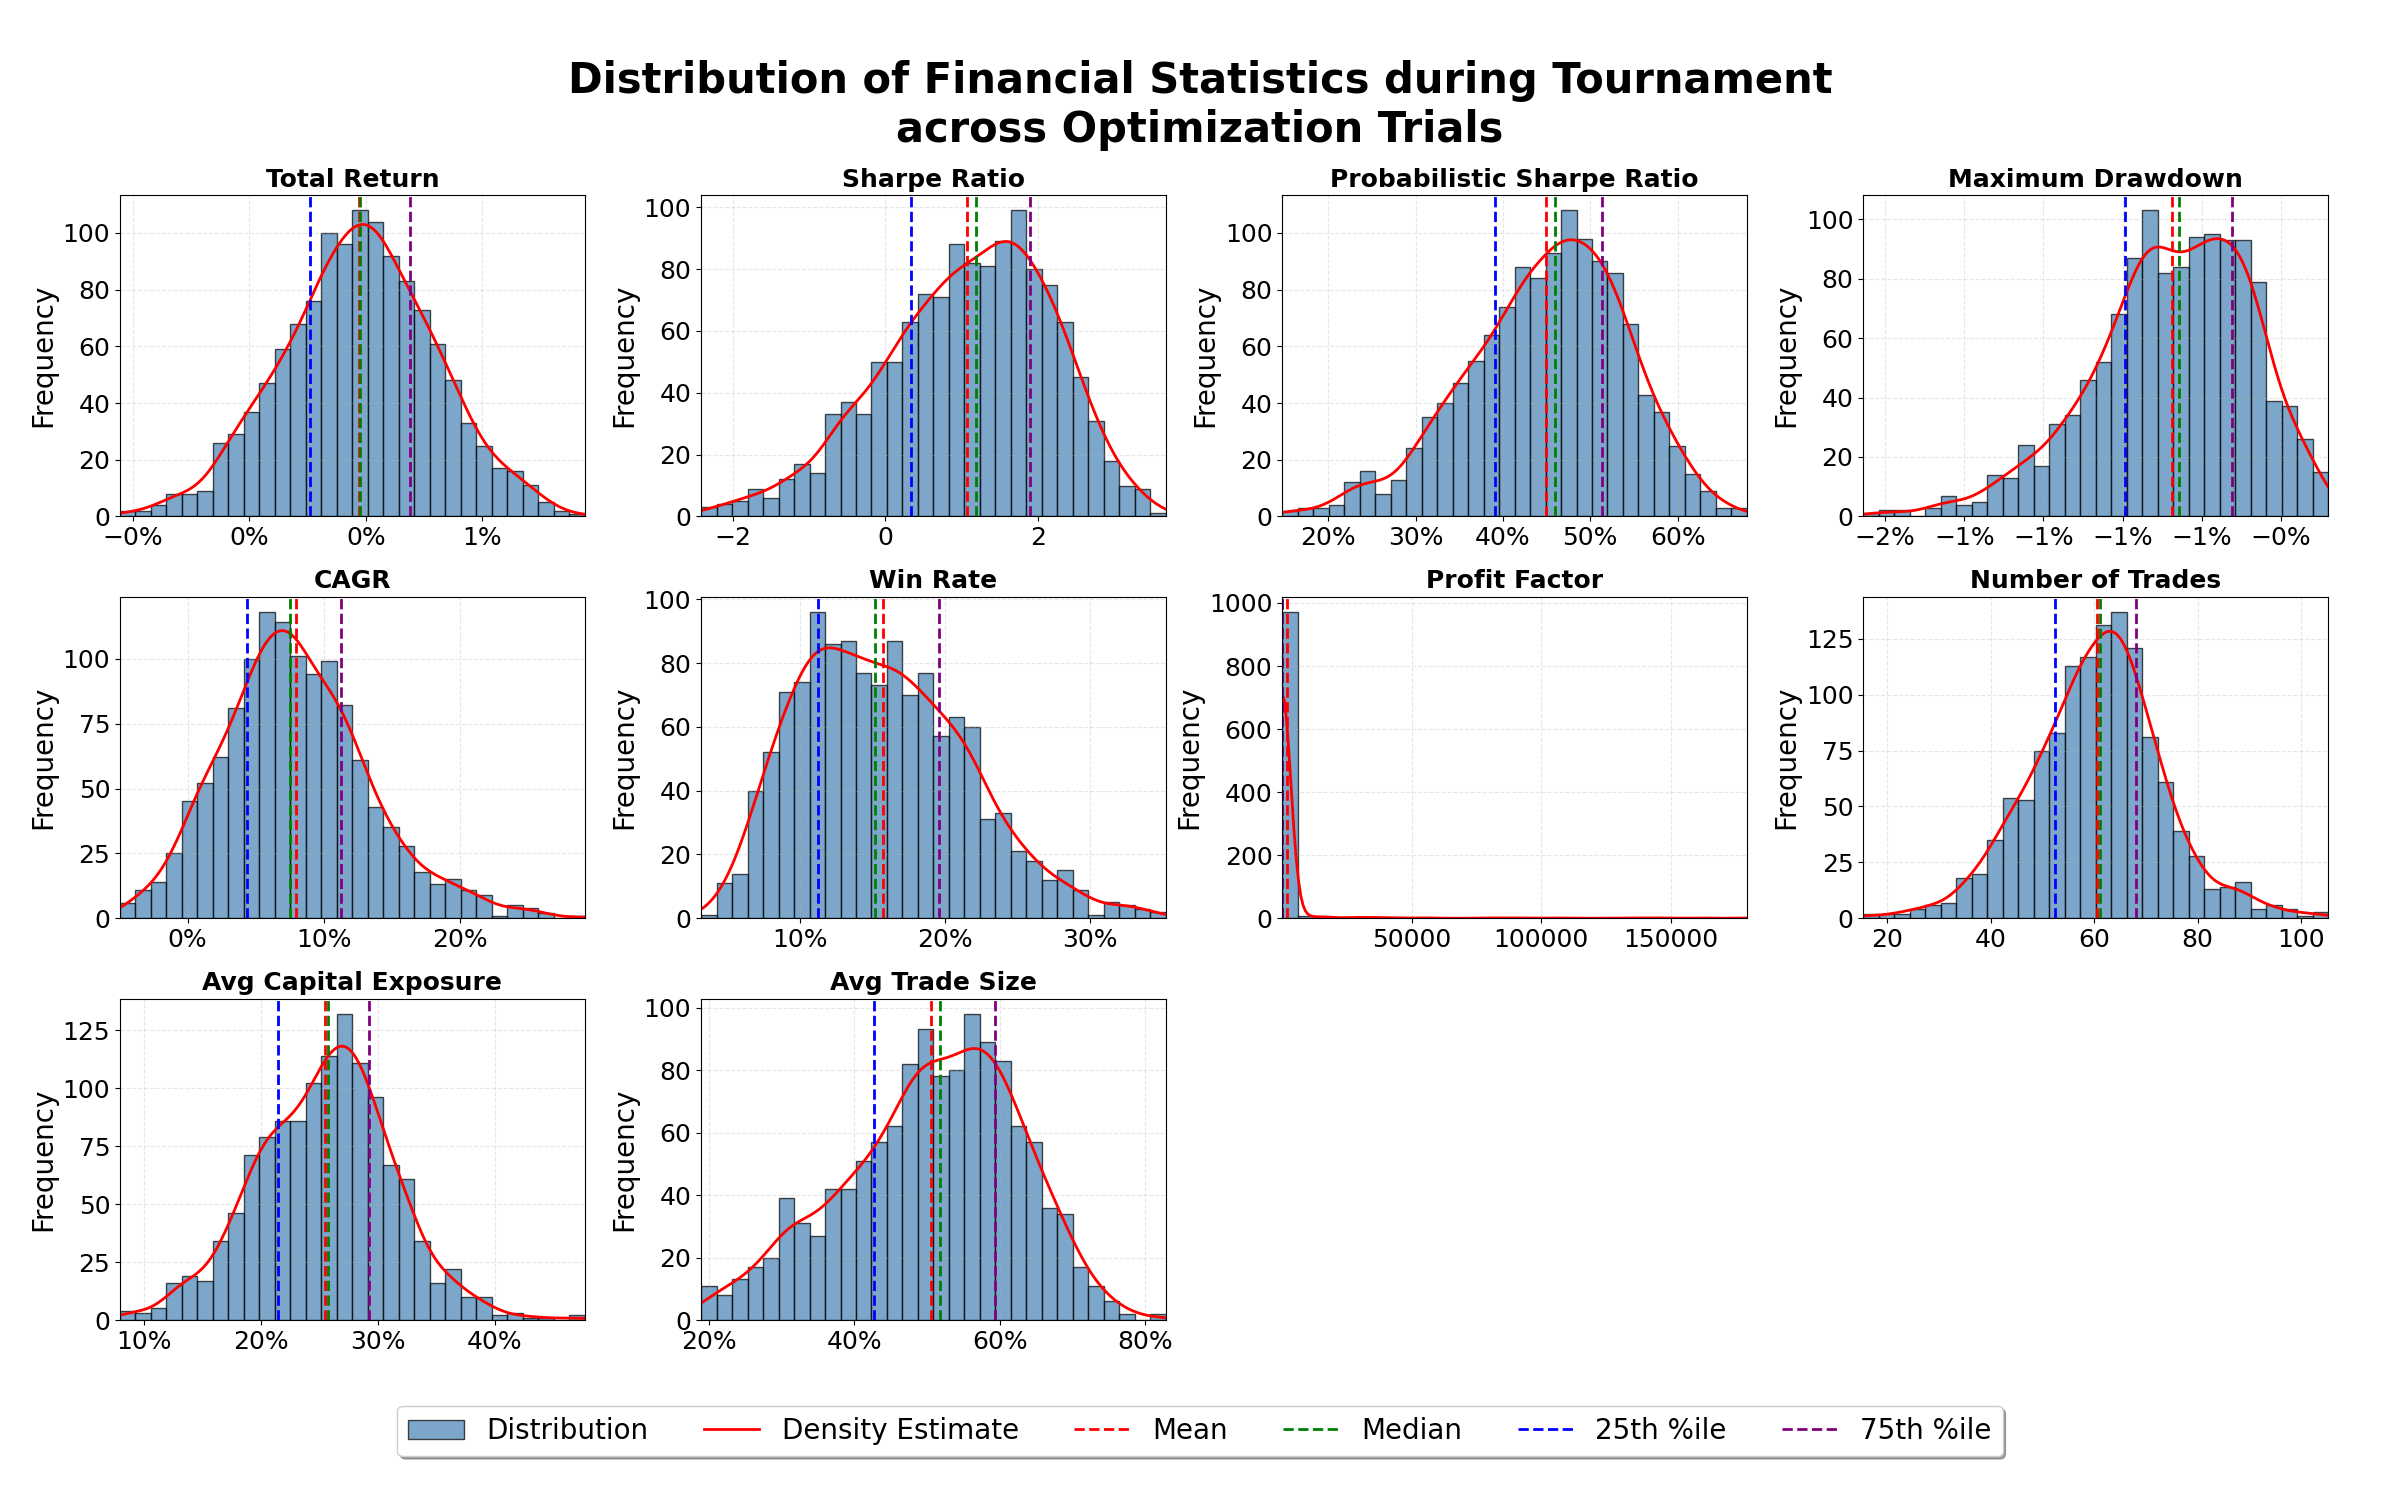
\includegraphics[width=0.95\linewidth]{../data/figures/optimization/distributions/Tournament_financial_dist_XGBoost.png}
    \caption{Financial Statistic Distributions During Tournament Optimization}
    \label{fig:distributions}
\end{figure}

Before discussing individual panels, it is worth clarifying how each point in \ref{fig:financial_dist_xgboost} is constructed. Rather than reporting one distribution per currency 
pair (which, across eleven pairs and two folds, would be prohibitively repetitive), each plotted trial value is the arithmetic mean of that trial's statistic across all pairs and 
all inner cross-validation folds evaluated during the trading-level Optuna search. This aggregation is what makes a single set of panels representative of the whole tournament, 
but it also has a direct bearing on the Profit Factor panel discussed below.

\medskip

Figure \ref{fig:financial_dist_xgboost} moves beyond the single best-performing configuration reported in table \ref{tab:hps_XGBoost_tournament} and examines the distribution of financial 
outcomes across the entire population of trading-hyperparameter trials sampled during the Optuna search. 
Encouragingly, Total Return, Sharpe Ratio, and CAGR all have the bulk of their mass sitting on the positive side of zero, indicating that a large fraction of the sampled 
hyperparameter space produces a modestly positive edge, at least during backtesting. 
The probabilistic Sharpe ratio panel tempers this reading, however, as its distribution is centered close to, and partially below, the $50\%$ mark, 
meaning that for a substantial share of trials the estimated Sharpe ratio would not be considered statistically distinguishable from zero once estimation uncertainty, skewness, 
and kurtosis are accounted for (see eq. \ref{eq:psr} in section \ref{sec:backtest_overfitting}). This is an important caveat to the otherwise favorable Sharpe and CAGR distributions as 
it suggests that while positive point estimates are common across the search space, robustly significant outperformance is concentrated in a comparatively narrower right-hand tail of trials.

\medskip

The Profit Factor panel exhibits an extreme long right tail, with the overwhelming majority of trials clustering near a small finite value and a sparse scattering of trials 
reporting values in the tens of thousands. This is not indicative of genuinely exceptional trading performance but rather a well-known degenerate artifact of the profit factor 
metric under low trade counts, propagated through an unweighted cross-pair average. Thus, a single pair that happens, under a given trial's sampled hyperparameters, to record only 
one or two winning trades and no losing trades in the evaluation window returns a profit factor that is undefined in the limit and numerically enormous in practice — a pathology 
already visible for several low-trade-count pairs in the individual tournament results (see appendix \ref{app:model_specific_backtests}). Because the plotted value is a 
simple mean across all pairs rather than a trade-count weighted one, a single such pair is sufficient to drag an otherwise unremarkable trial's reported profit factor into the tens 
of thousands, which is why the panel's tail is so extreme relative to its bulk. The Number of Trades and Win Rate panels support this interpretation as both report cross-pair and fold 
average values, clustering around $60$-$70$ trades with a left-skewed tail and a right-skewed win rate in the $10$-$20\%$ range, consistent with a trend-following, 
asymmetric-payoff style of strategy in which most individual trades lose small amounts and profitability is carried by a minority of large winners, which is precisely the regime 
in which individual pairs, and by extension the cross-pair mean, are most sensitive to small-sample noise in the profit factor. 
Finally, the Average Capital Exposure panel, which, unlike Max Exp. in \ref{tab:hps_XGBoost_tournament}, reflects the mean realized, mark-to-market exposure rather than the 
permitted ceiling, clusters around $25$-$30\%$, well below the $80$-$98\%$ ceilings frequently discovered by the optimizer. This gap indicates that the position sizing scaled by 
the Kelly fraction, rather than the notional exposure cap itself, is the binding constraint for most trials, with the exposure ceiling instead functioning as a rarely-triggered 
backstop against adverse mark-to-market drift rather than a target the strategy actively pushes toward.


\subsubsection{From Raw Signals to Conformal Predictions: Model- \& Pair-Specific Conformal-Q Filtering}

%%%%%%%%%%%%%%%%%%%%%%%%%%%%%%%%%%%%%%%%%%%%%%%%%%%%%%%%%%%%%%%%%%%%%%%%%%%%%%%%%%%%%%%%%%%%%%%%%%%%%%%%%%%%%%%%%%%%%%%%%%%
%%%%%%%%%%%%%%%%%%%%%%%%%%%%%%%%%%%%%%%%%%%%%%%%%%%%%%%%%%%%%%%%%%%%%%%%%%%%%%%%%%%%%%%%%%%%%%%%%%%%%%%%%%%%%%%%%%%%%%%%%%%
Lorem ipsum dolor sit amet, consectetur adipiscing elit. Sed do eiusmod tempor incididunt ut labore et dolore magna aliqua. 
Ut enim ad minim veniam, quis nostrud exercitation ullamco laboris nisi ut aliquip ex ea commodo consequat. 
Duis aute irure dolor in reprehenderit in voluptate velit esse cillum dolore eu fugiat nulla pariatur. 
Excepteur sint occaecat cupidatat non proident, sunt in culpa qui officia deserunt mollit anim id est laborum
Lorem ipsum dolor sit amet, consectetur adipiscing elit. Sed do eiusmod tempor incididunt ut labore et dolore magna aliqua. 
Ut enim ad minim veniam, quis nostrud exercitation ullamco laboris nisi ut aliquip ex ea commodo consequat. 
Duis aute irure dolor in reprehenderit in voluptate velit esse cillum dolore eu fugiat nulla pariatur. 
Excepteur sint occaecat cupidatat non proident, sunt in culpa qui officia deserunt mollit anim id est laborum
Lorem ipsum dolor sit amet, consectetur adipiscing elit. Sed do eiusmod tempor incididunt ut labore et dolore magna aliqua. 
Ut enim ad minim veniam, quis nostrud exercitation ullamco laboris nisi ut aliquip ex ea commodo consequat. 
Duis aute irure dolor in reprehenderit in voluptate velit esse cillum dolore eu fugiat nulla pariatur. 
Excepteur sint occaecat cupidatat non proident, sunt in culpa qui officia deserunt mollit anim id est laborum
%%%%%%%%%%%%%%%%%%%%%%%%%%%%%%%%%%%%%%%%%%%%%%%%%%%%%%%%%%%%%%%%%%%%%%%%%%%%%%%%%%%%%%%%%%%%%%%%%%%%%%%%%%%%%%%%%%%%%%%%%%%
%%%%%%%%%%%%%%%%%%%%%%%%%%%%%%%%%%%%%%%%%%%%%%%%%%%%%%%%%%%%%%%%%%%%%%%%%%%%%%%%%%%%%%%%%%%%%%%%%%%%%%%%%%%%%%%%%%%%%%%%%%%

\begin{figure}[H]
    \centering
    \begin{minipage}[t]{0.49\textwidth}
        \centering
        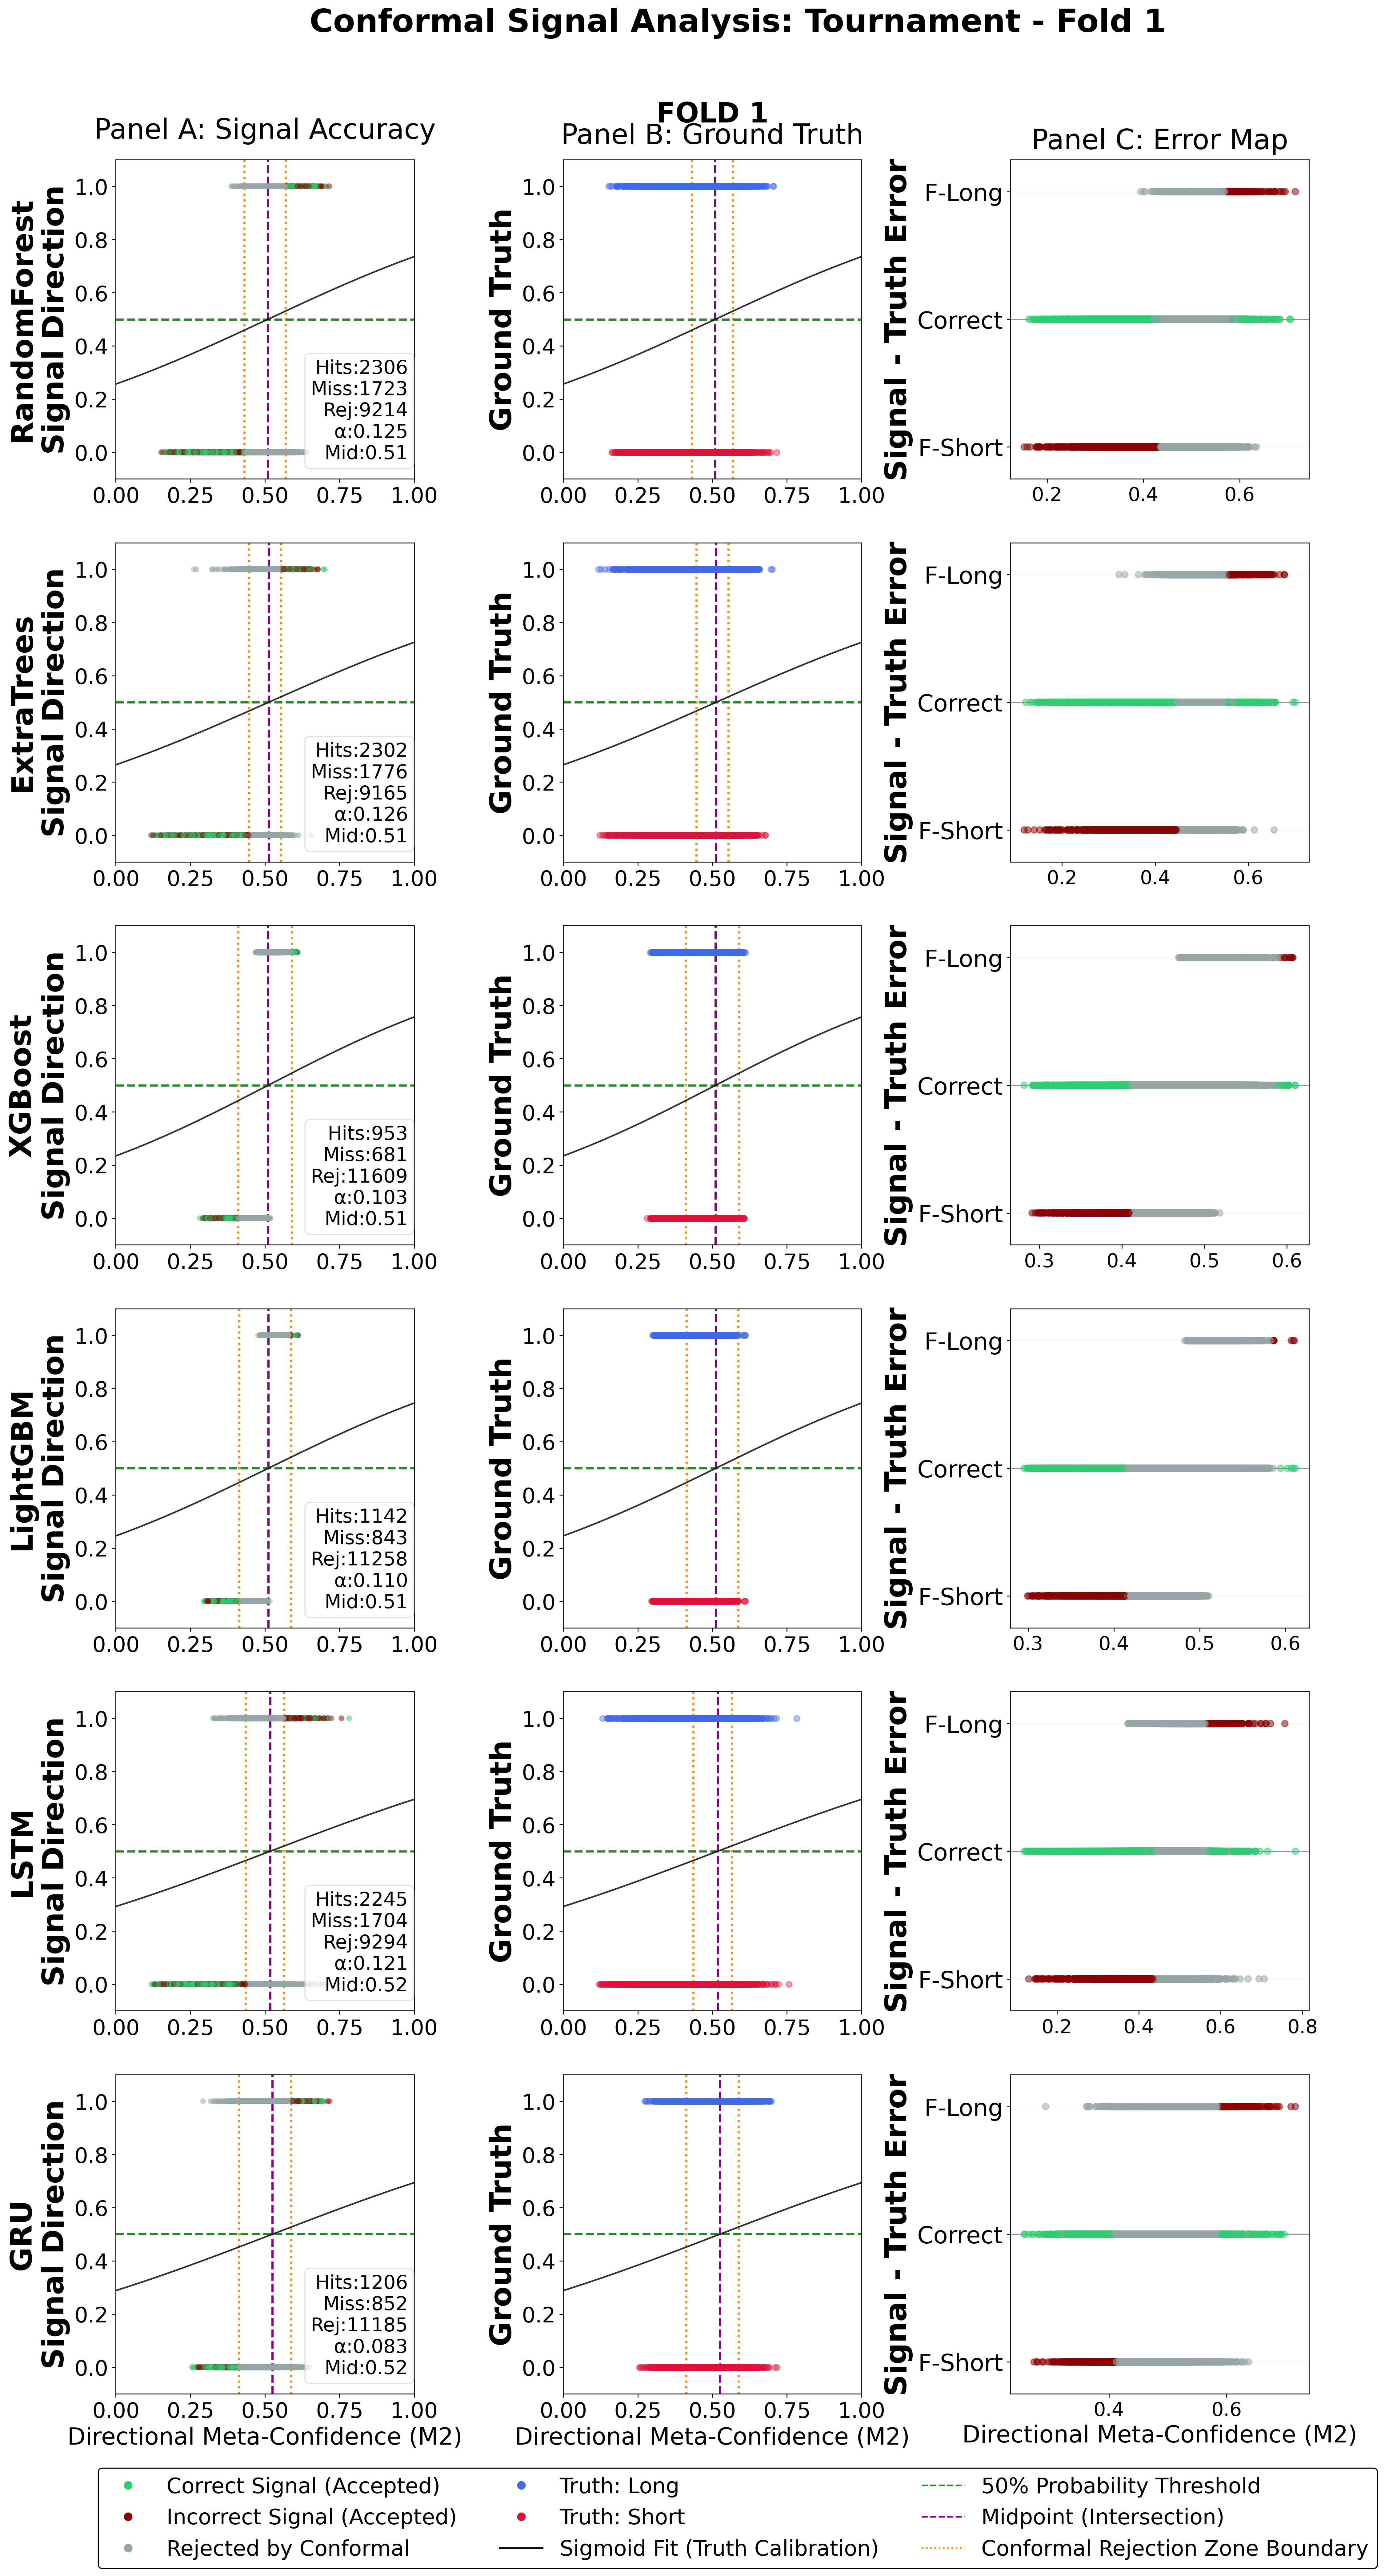
\includegraphics[width=\textwidth]{../data/figures/conformal_predictions/Tournament_conformal_predictions_part1.png}
        \caption{Model-Specific Conformal Filtering During Tournament}
        \label{fig:model-specific conformal filtering 1}
    \end{minipage}
    \hfill
    \begin{minipage}[t]{0.49\textwidth}
        \centering
        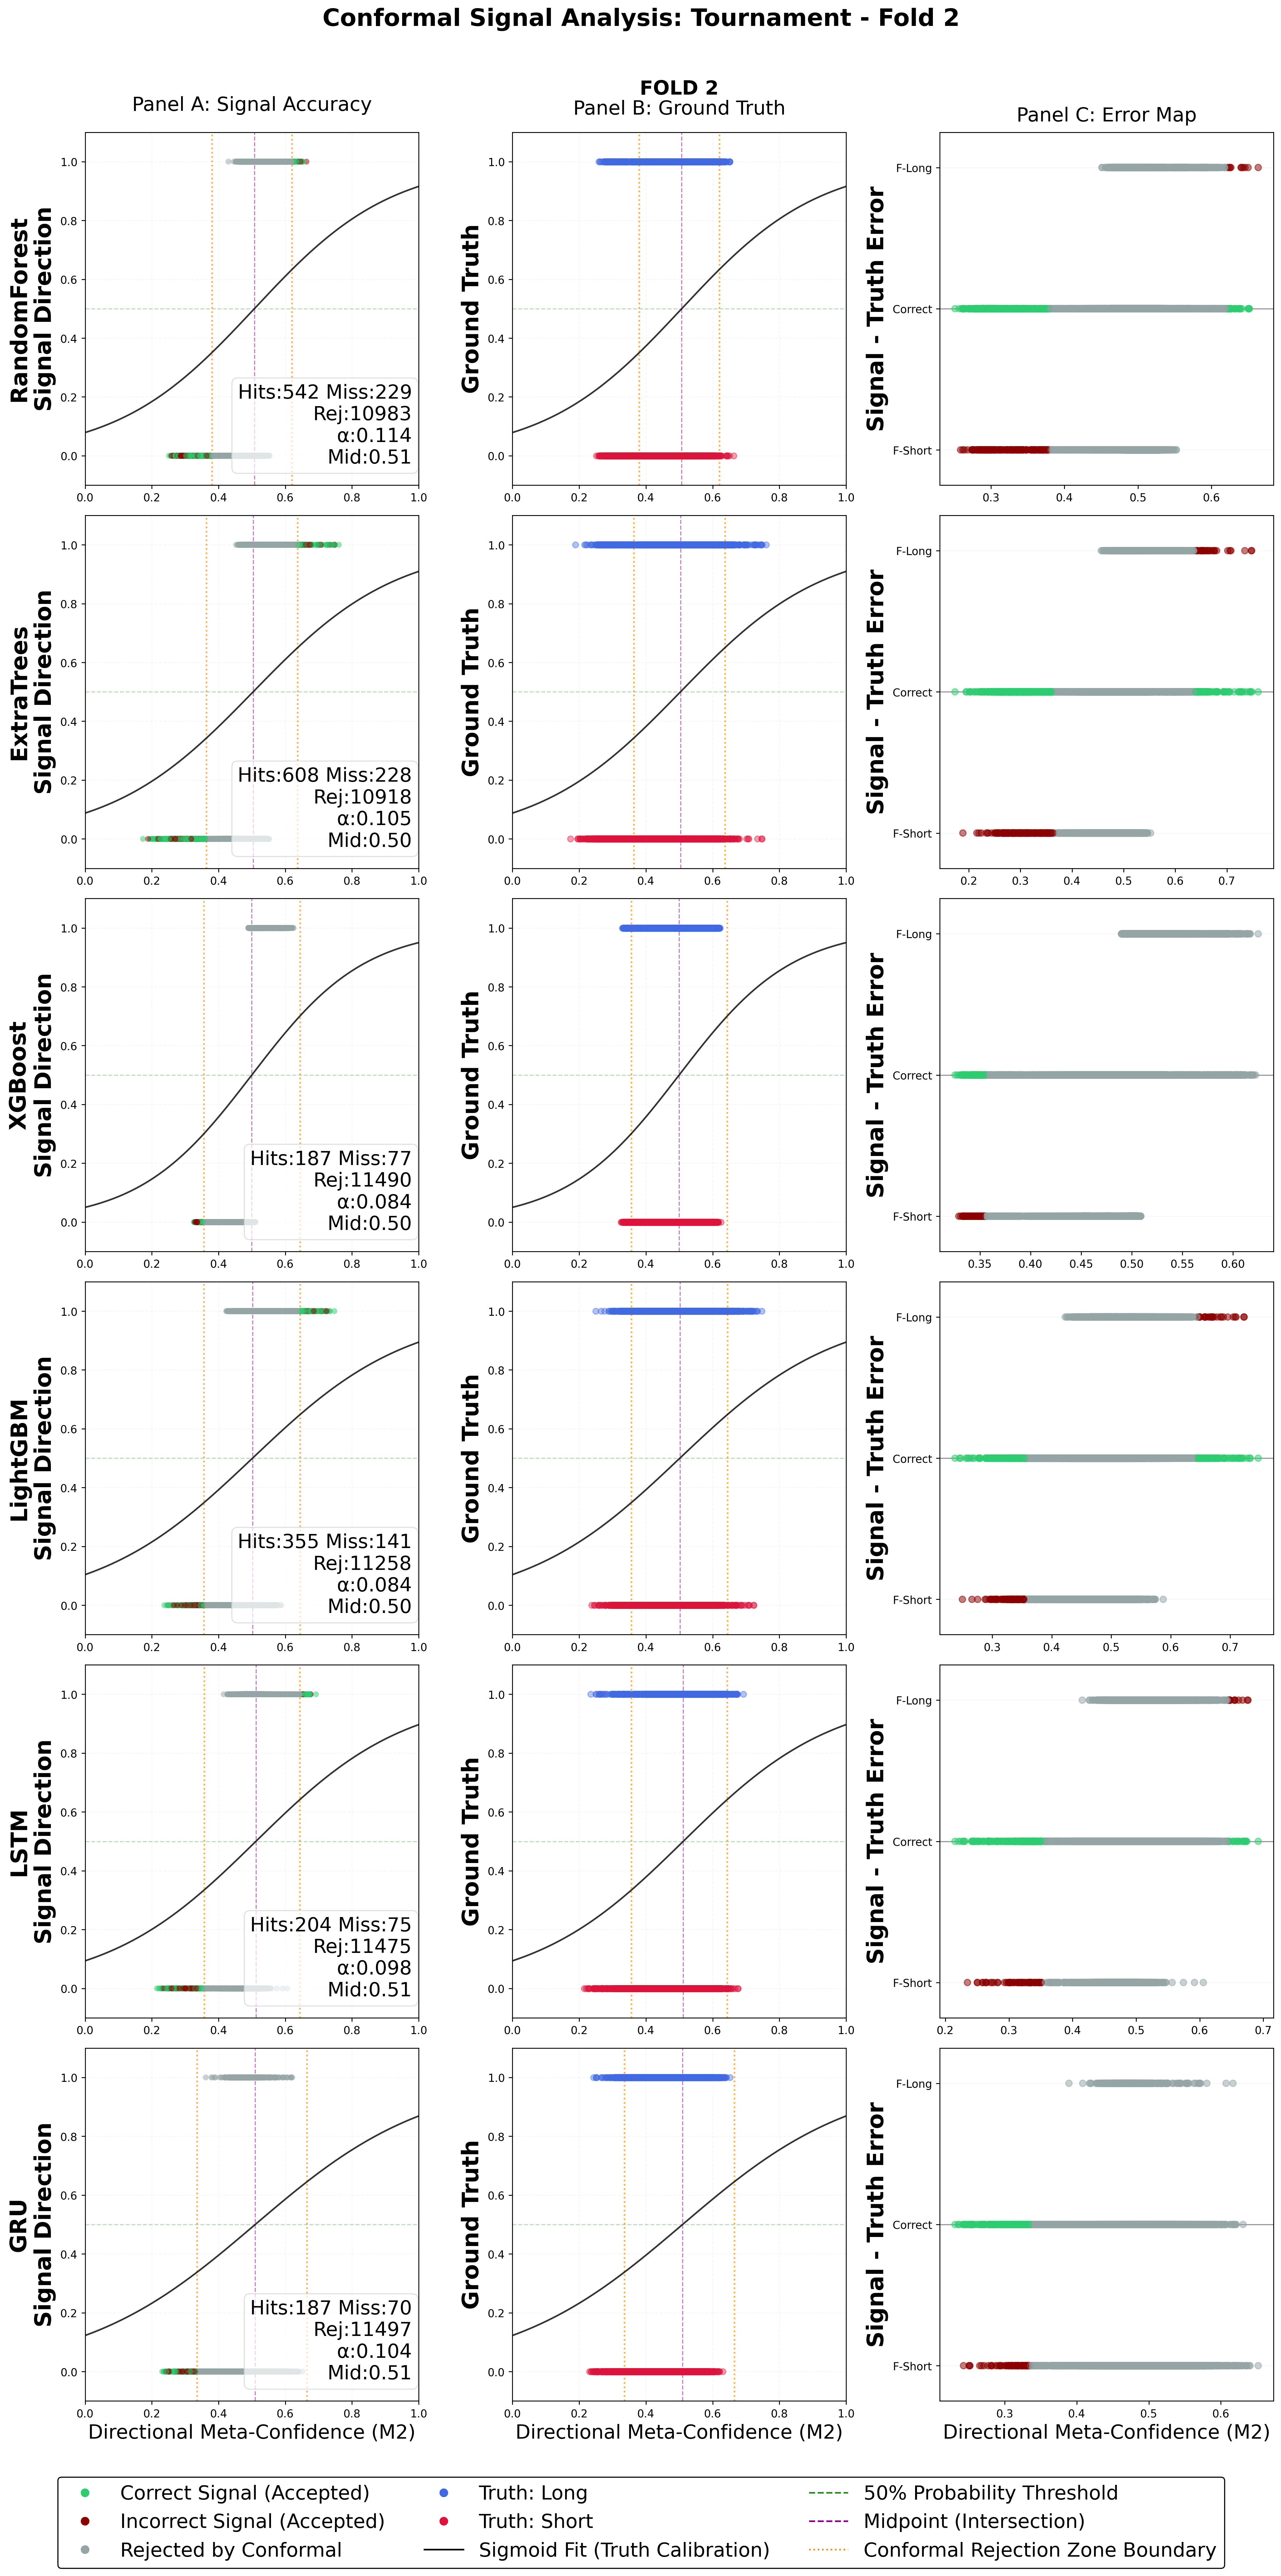
\includegraphics[width=\textwidth]{../data/figures/conformal_predictions/Tournament_conformal_predictions_part2.png}
        \caption{Model-Specific Conformal Filtering During Tournament (Continued)}
        \label{fig:model-specific conformal filtering 2}
    \end{minipage}
\end{figure}

%%%%%%%%%%%%%%%%%%%%%%%%%%%%%%%%%%%%%%%%%%%%%%%%%%%%%%%%%%%%%%%%%%%%%%%%%%%%%%%%%%%%%%%%%%%%%%%%%%%%%%%%%%%%%%%%%%%%%%%%%%%
%%%%%%%%%%%%%%%%%%%%%%%%%%%%%%%%%%%%%%%%%%%%%%%%%%%%%%%%%%%%%%%%%%%%%%%%%%%%%%%%%%%%%%%%%%%%%%%%%%%%%%%%%%%%%%%%%%%%%%%%%%%
Lorem ipsum dolor sit amet, consectetur adipiscing elit. Sed do eiusmod tempor incididunt ut labore et dolore magna aliqua. 
Ut enim ad minim veniam, quis nostrud exercitation ullamco laboris nisi ut aliquip ex ea commodo consequat. 
Duis aute irure dolor in reprehenderit in voluptate velit esse cillum dolore eu fugiat nulla pariatur. 
Excepteur sint occaecat cupidatat non proident, sunt in culpa qui officia deserunt mollit anim id est laborum
Lorem ipsum dolor sit amet, consectetur adipiscing elit. Sed do eiusmod tempor incididunt ut labore et dolore magna aliqua. 
Ut enim ad minim veniam, quis nostrud exercitation ullamco laboris nisi ut aliquip ex ea commodo consequat. 
Duis aute irure dolor in reprehenderit in voluptate velit esse cillum dolore eu fugiat nulla pariatur. 
Excepteur sint occaecat cupidatat non proident, sunt in culpa qui officia deserunt mollit anim id est laborum
Lorem ipsum dolor sit amet, consectetur adipiscing elit. Sed do eiusmod tempor incididunt ut labore et dolore magna aliqua. 
Ut enim ad minim veniam, quis nostrud exercitation ullamco laboris nisi ut aliquip ex ea commodo consequat. 
Duis aute irure dolor in reprehenderit in voluptate velit esse cillum dolore eu fugiat nulla pariatur. 
Excepteur sint occaecat cupidatat non proident, sunt in culpa qui officia deserunt mollit anim id est laborum
%%%%%%%%%%%%%%%%%%%%%%%%%%%%%%%%%%%%%%%%%%%%%%%%%%%%%%%%%%%%%%%%%%%%%%%%%%%%%%%%%%%%%%%%%%%%%%%%%%%%%%%%%%%%%%%%%%%%%%%%%%%
%%%%%%%%%%%%%%%%%%%%%%%%%%%%%%%%%%%%%%%%%%%%%%%%%%%%%%%%%%%%%%%%%%%%%%%%%%%%%%%%%%%%%%%%%%%%%%%%%%%%%%%%%%%%%%%%%%%%%%%%%%%


\subsubsection{Validation of Conformal-Q Filtering: Model- and Fold-Specific Confusion Matrices \& Calibration}

%%%%%%%%%%%%%%%%%%%%%%%%%%%%%%%%%%%%%%%%%%%%%%%%%%%%%%%%%%%%%%%%%%%%%%%%%%%%%%%%%%%%%%%%%%%%%%%%%%%%%%%%%%%%%%%%%%%%%%%%%%%
%%%%%%%%%%%%%%%%%%%%%%%%%%%%%%%%%%%%%%%%%%%%%%%%%%%%%%%%%%%%%%%%%%%%%%%%%%%%%%%%%%%%%%%%%%%%%%%%%%%%%%%%%%%%%%%%%%%%%%%%%%%
Lorem ipsum dolor sit amet, consectetur adipiscing elit. Sed do eiusmod tempor incididunt ut labore et dolore magna aliqua. 
Ut enim ad minim veniam, quis nostrud exercitation ullamco laboris nisi ut aliquip ex ea commodo consequat. 
Duis aute irure dolor in reprehenderit in voluptate velit esse cillum dolore eu fugiat nulla pariatur. 
Excepteur sint occaecat cupidatat non proident, sunt in culpa qui officia deserunt mollit anim id est laborum
Lorem ipsum dolor sit amet, consectetur adipiscing elit. Sed do eiusmod tempor incididunt ut labore et dolore magna aliqua. 
Ut enim ad minim veniam, quis nostrud exercitation ullamco laboris nisi ut aliquip ex ea commodo consequat. 
Duis aute irure dolor in reprehenderit in voluptate velit esse cillum dolore eu fugiat nulla pariatur. 
Excepteur sint occaecat cupidatat non proident, sunt in culpa qui officia deserunt mollit anim id est laborum
Lorem ipsum dolor sit amet, consectetur adipiscing elit. Sed do eiusmod tempor incididunt ut labore et dolore magna aliqua. 
Ut enim ad minim veniam, quis nostrud exercitation ullamco laboris nisi ut aliquip ex ea commodo consequat. 
Duis aute irure dolor in reprehenderit in voluptate velit esse cillum dolore eu fugiat nulla pariatur. 
Excepteur sint occaecat cupidatat non proident, sunt in culpa qui officia deserunt mollit anim id est laborum
%%%%%%%%%%%%%%%%%%%%%%%%%%%%%%%%%%%%%%%%%%%%%%%%%%%%%%%%%%%%%%%%%%%%%%%%%%%%%%%%%%%%%%%%%%%%%%%%%%%%%%%%%%%%%%%%%%%%%%%%%%%
%%%%%%%%%%%%%%%%%%%%%%%%%%%%%%%%%%%%%%%%%%%%%%%%%%%%%%%%%%%%%%%%%%%%%%%%%%%%%%%%%%%%%%%%%%%%%%%%%%%%%%%%%%%%%%%%%%%%%%%%%%%


\paragraph{Confusion Matrices}

\begin{figure}[H]
    \centering
    \begin{minipage}[t]{0.49\textwidth}
        \centering
        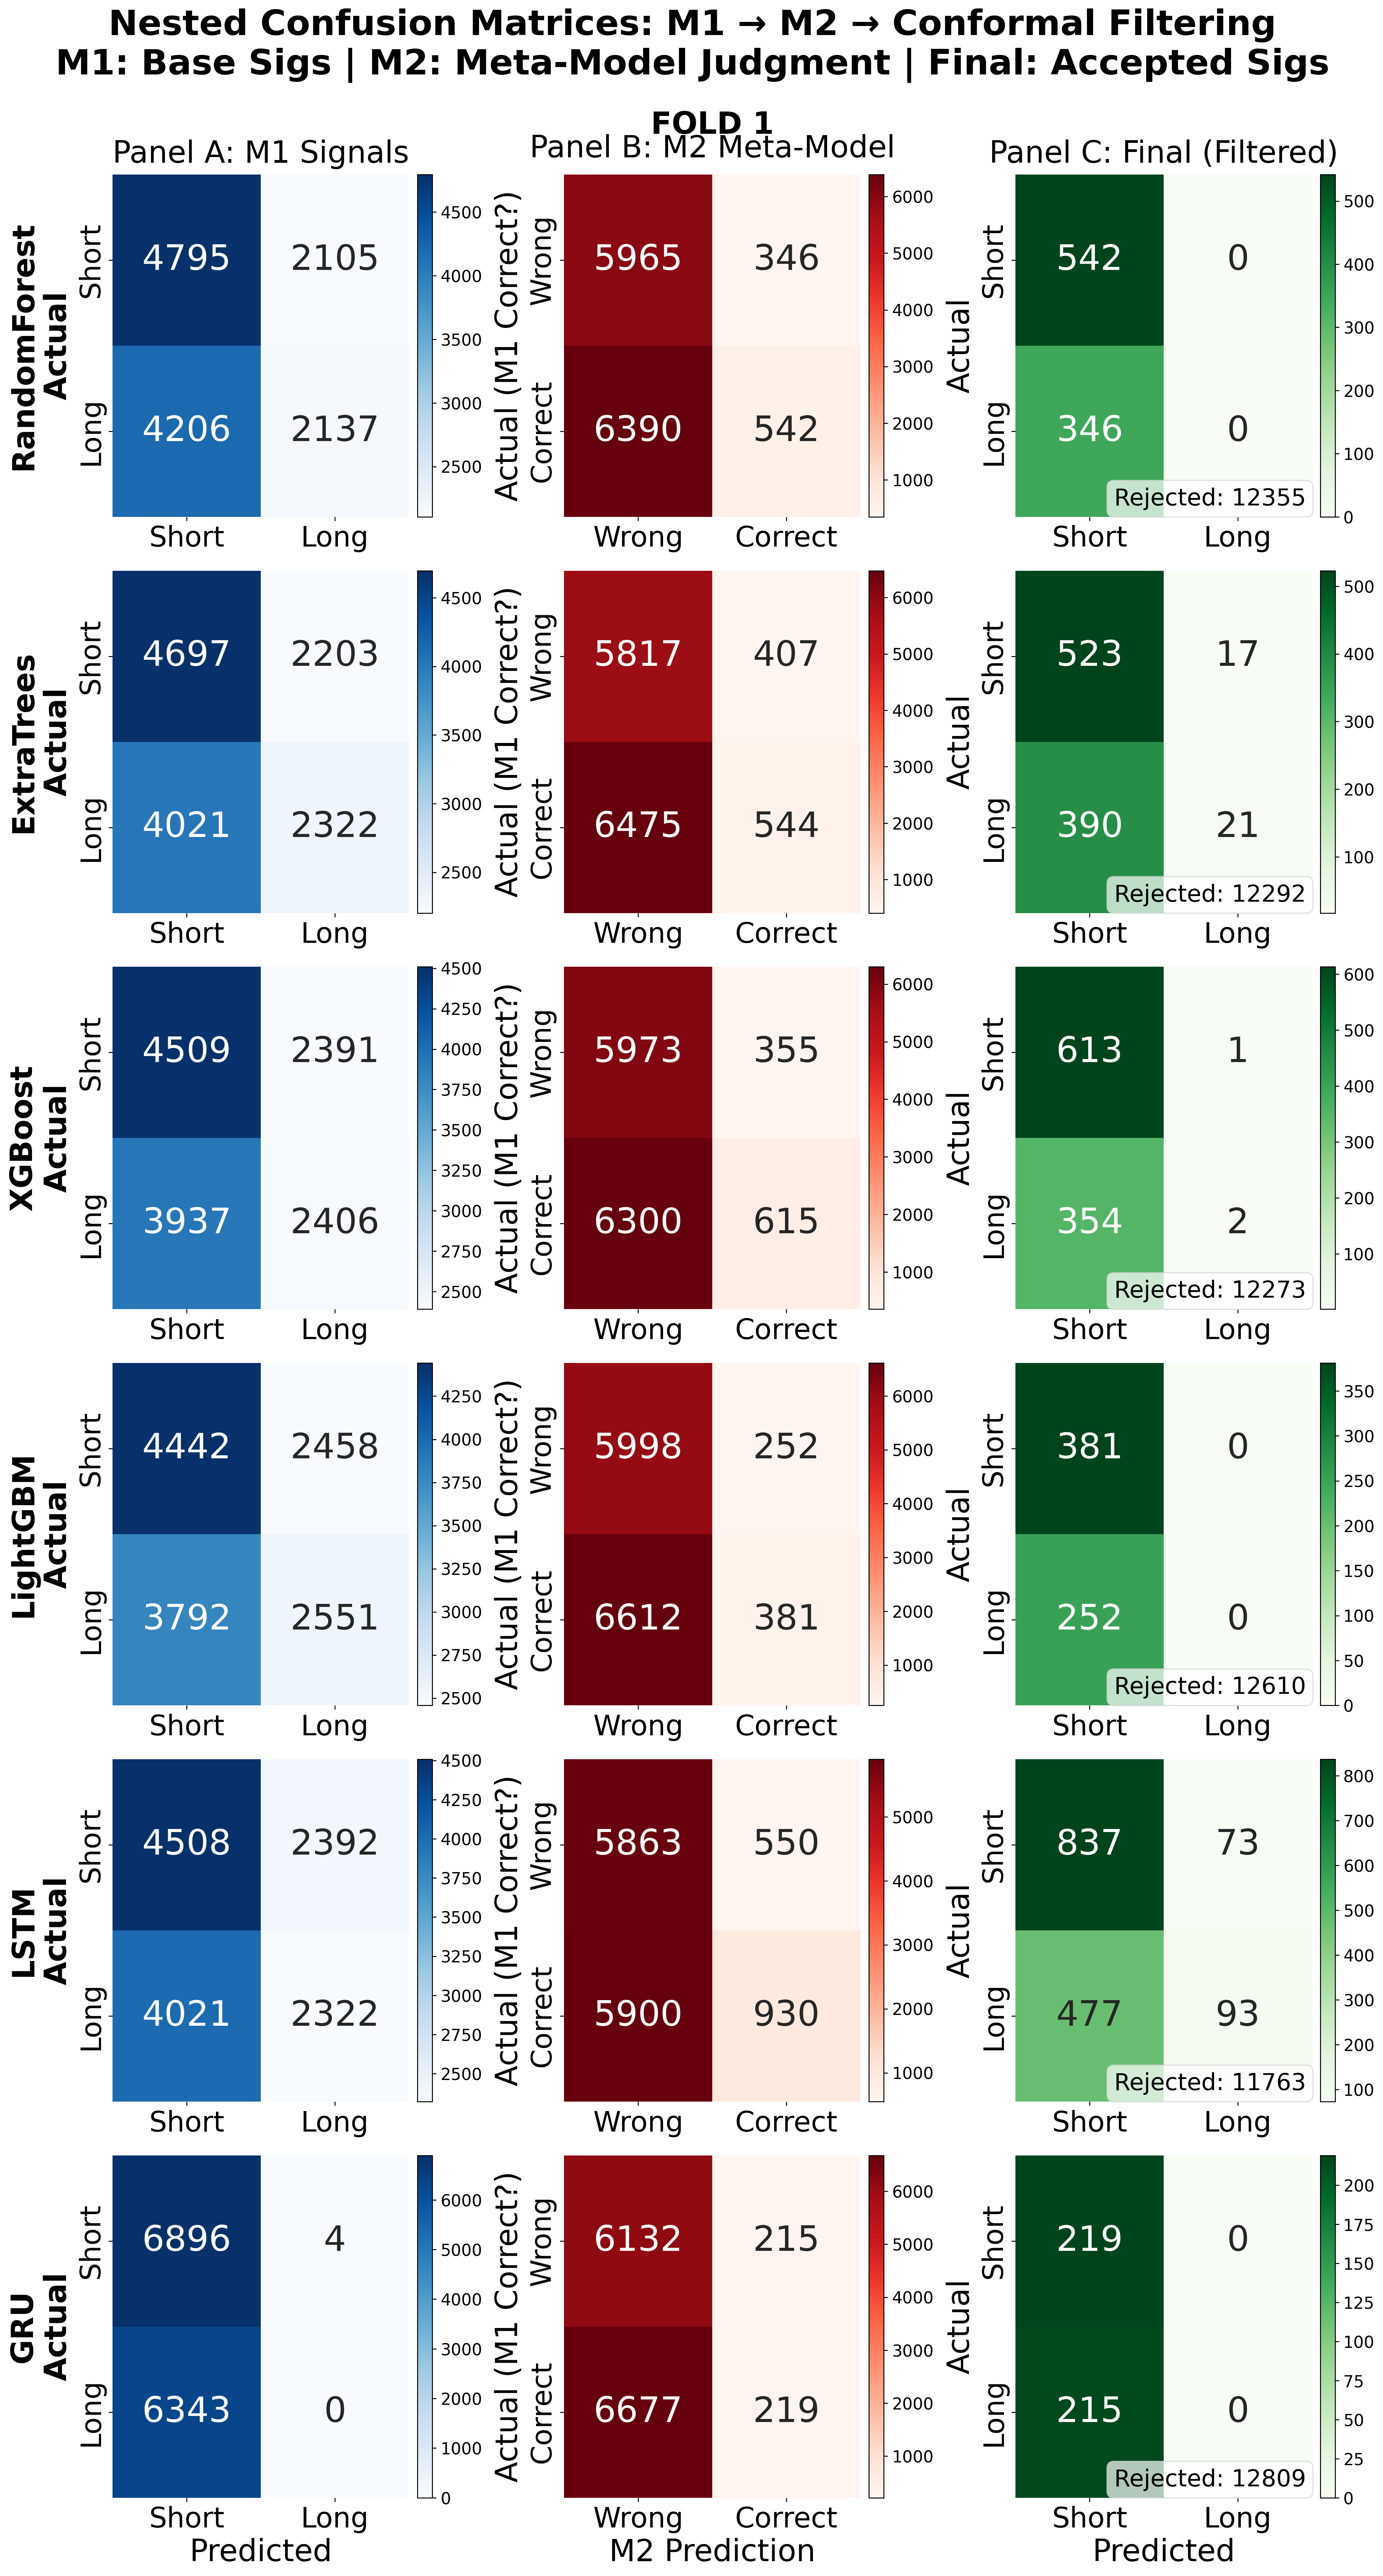
\includegraphics[width=\textwidth]{../data/figures/confusion_matrices/Tournament_nested_confusion_matrices_part1.png}
        \caption{Model-Specific Confusion Matrices During Tournament}
        \label{fig:model-specific confusion matrices 1}
    \end{minipage}
    \hfill
    \begin{minipage}[t]{0.49\textwidth}
        \centering
        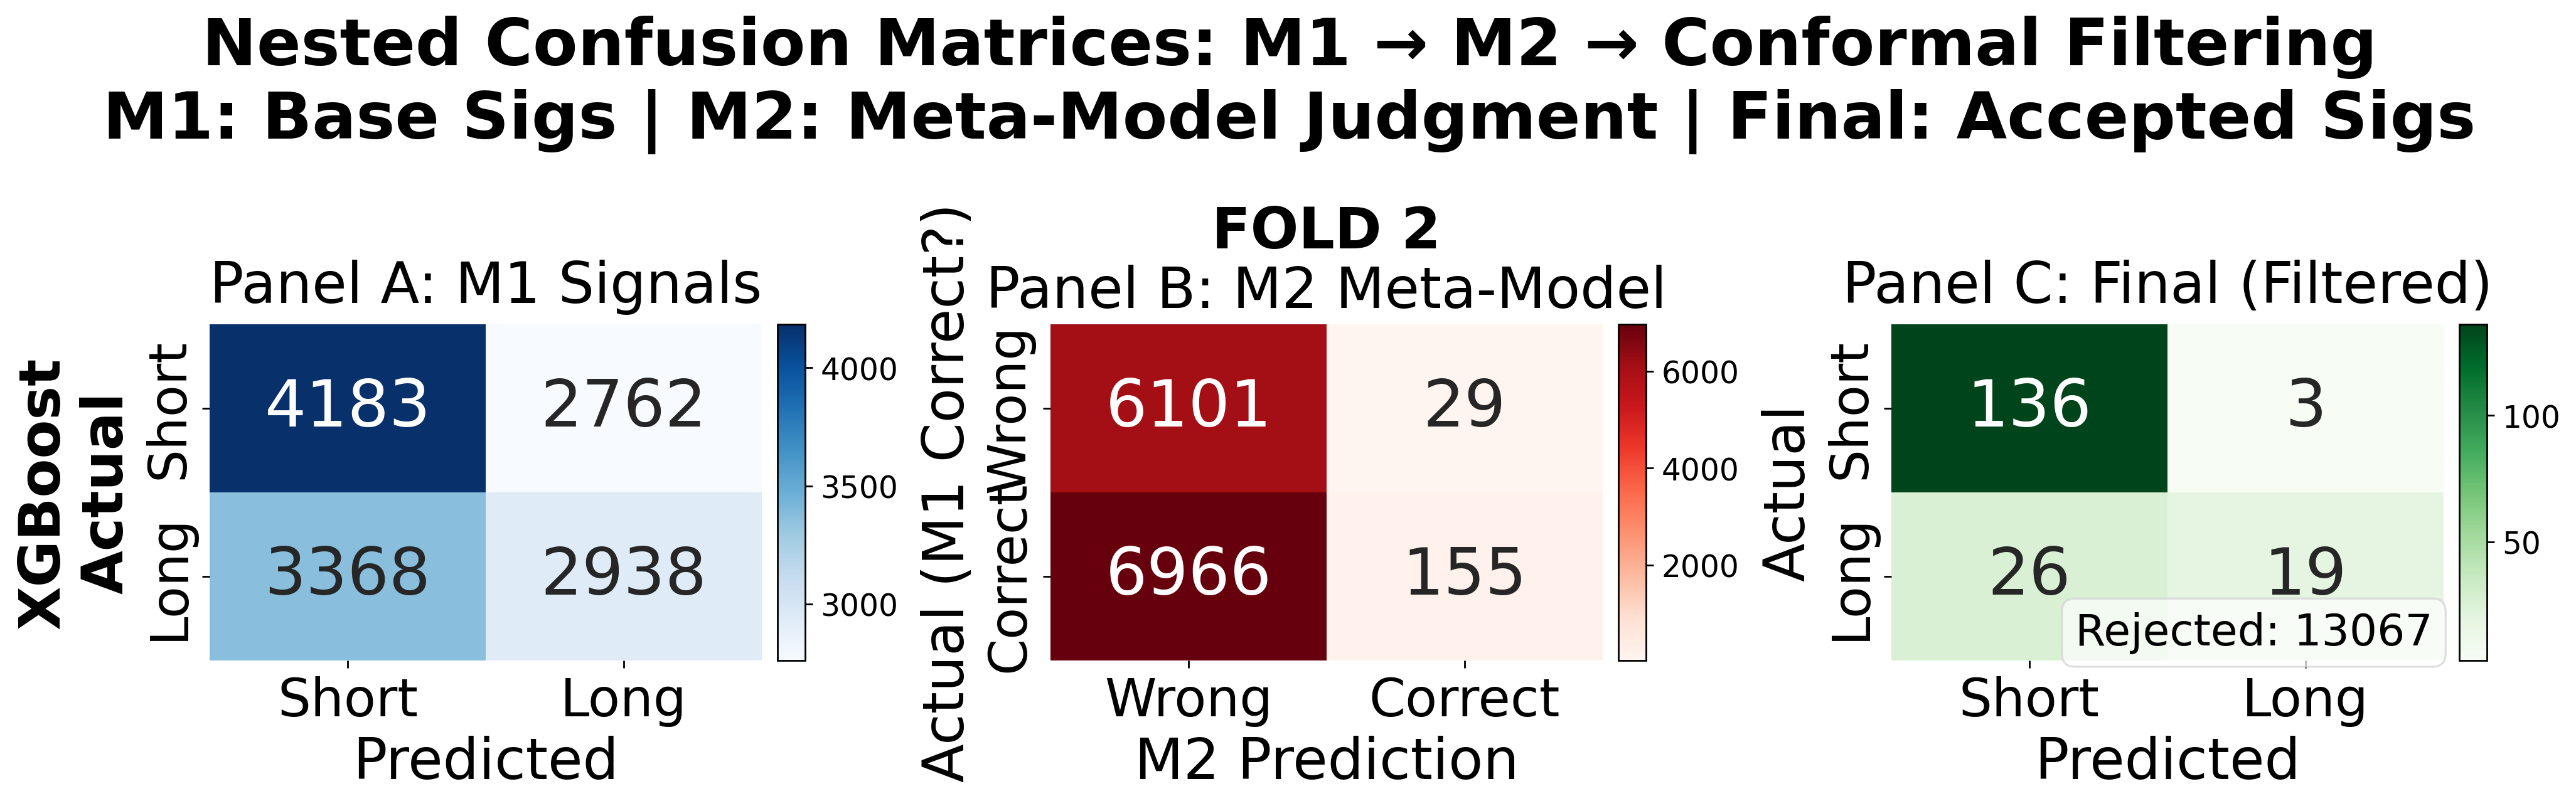
\includegraphics[width=\textwidth]{../data/figures/confusion_matrices/Tournament_nested_confusion_matrices_part2.png}
        \caption{Model-Specific Confusion Matrices During Tournament (Continued)}
        \label{fig:model-specific confusion matrices 2}
    \end{minipage}
\end{figure}

%%%%%%%%%%%%%%%%%%%%%%%%%%%%%%%%%%%%%%%%%%%%%%%%%%%%%%%%%%%%%%%%%%%%%%%%%%%%%%%%%%%%%%%%%%%%%%%%%%%%%%%%%%%%%%%%%%%%%%%%%%%
%%%%%%%%%%%%%%%%%%%%%%%%%%%%%%%%%%%%%%%%%%%%%%%%%%%%%%%%%%%%%%%%%%%%%%%%%%%%%%%%%%%%%%%%%%%%%%%%%%%%%%%%%%%%%%%%%%%%%%%%%%%
Lorem ipsum dolor sit amet, consectetur adipiscing elit. Sed do eiusmod tempor incididunt ut labore et dolore magna aliqua. 
Ut enim ad minim veniam, quis nostrud exercitation ullamco laboris nisi ut aliquip ex ea commodo consequat. 
Duis aute irure dolor in reprehenderit in voluptate velit esse cillum dolore eu fugiat nulla pariatur. 
Excepteur sint occaecat cupidatat non proident, sunt in culpa qui officia deserunt mollit anim id est laborum
Lorem ipsum dolor sit amet, consectetur adipiscing elit. Sed do eiusmod tempor incididunt ut labore et dolore magna aliqua. 
Ut enim ad minim veniam, quis nostrud exercitation ullamco laboris nisi ut aliquip ex ea commodo consequat. 
Duis aute irure dolor in reprehenderit in voluptate velit esse cillum dolore eu fugiat nulla pariatur. 
Excepteur sint occaecat cupidatat non proident, sunt in culpa qui officia deserunt mollit anim id est laborum
Lorem ipsum dolor sit amet, consectetur adipiscing elit. Sed do eiusmod tempor incididunt ut labore et dolore magna aliqua. 
Ut enim ad minim veniam, quis nostrud exercitation ullamco laboris nisi ut aliquip ex ea commodo consequat. 
Duis aute irure dolor in reprehenderit in voluptate velit esse cillum dolore eu fugiat nulla pariatur. 
Excepteur sint occaecat cupidatat non proident, sunt in culpa qui officia deserunt mollit anim id est laborum
%%%%%%%%%%%%%%%%%%%%%%%%%%%%%%%%%%%%%%%%%%%%%%%%%%%%%%%%%%%%%%%%%%%%%%%%%%%%%%%%%%%%%%%%%%%%%%%%%%%%%%%%%%%%%%%%%%%%%%%%%%%
%%%%%%%%%%%%%%%%%%%%%%%%%%%%%%%%%%%%%%%%%%%%%%%%%%%%%%%%%%%%%%%%%%%%%%%%%%%%%%%%%%%%%%%%%%%%%%%%%%%%%%%%%%%%%%%%%%%%%%%%%%%


\paragraph{Reliability Diagrams}

%%%%%%%%%%%%%%%%%%%%%%%%%%%%%%%%%%%%%%%%%%%%%%%%%%%%%%%%%%%%%%%%%%%%%%%%%%%%%%%%%%%%%%%%%%%%%%%%%%%%%%%%%%%%%%%%%%%%%%%%%%%
%%%%%%%%%%%%%%%%%%%%%%%%%%%%%%%%%%%%%%%%%%%%%%%%%%%%%%%%%%%%%%%%%%%%%%%%%%%%%%%%%%%%%%%%%%%%%%%%%%%%%%%%%%%%%%%%%%%%%%%%%%%
Lorem ipsum dolor sit amet, consectetur adipiscing elit. Sed do eiusmod tempor incididunt ut labore et dolore magna aliqua. 
Ut enim ad minim veniam, quis nostrud exercitation ullamco laboris nisi ut aliquip ex ea commodo consequat. 
Duis aute irure dolor in reprehenderit in voluptate velit esse cillum dolore eu fugiat nulla pariatur. 
Excepteur sint occaecat cupidatat non proident, sunt in culpa qui officia deserunt mollit anim id est laborum
Lorem ipsum dolor sit amet, consectetur adipiscing elit. Sed do eiusmod tempor incididunt ut labore et dolore magna aliqua. 
Ut enim ad minim veniam, quis nostrud exercitation ullamco laboris nisi ut aliquip ex ea commodo consequat. 
Duis aute irure dolor in reprehenderit in voluptate velit esse cillum dolore eu fugiat nulla pariatur. 
Excepteur sint occaecat cupidatat non proident, sunt in culpa qui officia deserunt mollit anim id est laborum
Lorem ipsum dolor sit amet, consectetur adipiscing elit. Sed do eiusmod tempor incididunt ut labore et dolore magna aliqua. 
Ut enim ad minim veniam, quis nostrud exercitation ullamco laboris nisi ut aliquip ex ea commodo consequat. 
Duis aute irure dolor in reprehenderit in voluptate velit esse cillum dolore eu fugiat nulla pariatur. 
Excepteur sint occaecat cupidatat non proident, sunt in culpa qui officia deserunt mollit anim id est laborum
%%%%%%%%%%%%%%%%%%%%%%%%%%%%%%%%%%%%%%%%%%%%%%%%%%%%%%%%%%%%%%%%%%%%%%%%%%%%%%%%%%%%%%%%%%%%%%%%%%%%%%%%%%%%%%%%%%%%%%%%%%%
%%%%%%%%%%%%%%%%%%%%%%%%%%%%%%%%%%%%%%%%%%%%%%%%%%%%%%%%%%%%%%%%%%%%%%%%%%%%%%%%%%%%%%%%%%%%%%%%%%%%%%%%%%%%%%%%%%%%%%%%%%%

\begin{figure}[H]
    \centering
    \begin{minipage}[t]{0.49\textwidth}
        \centering
        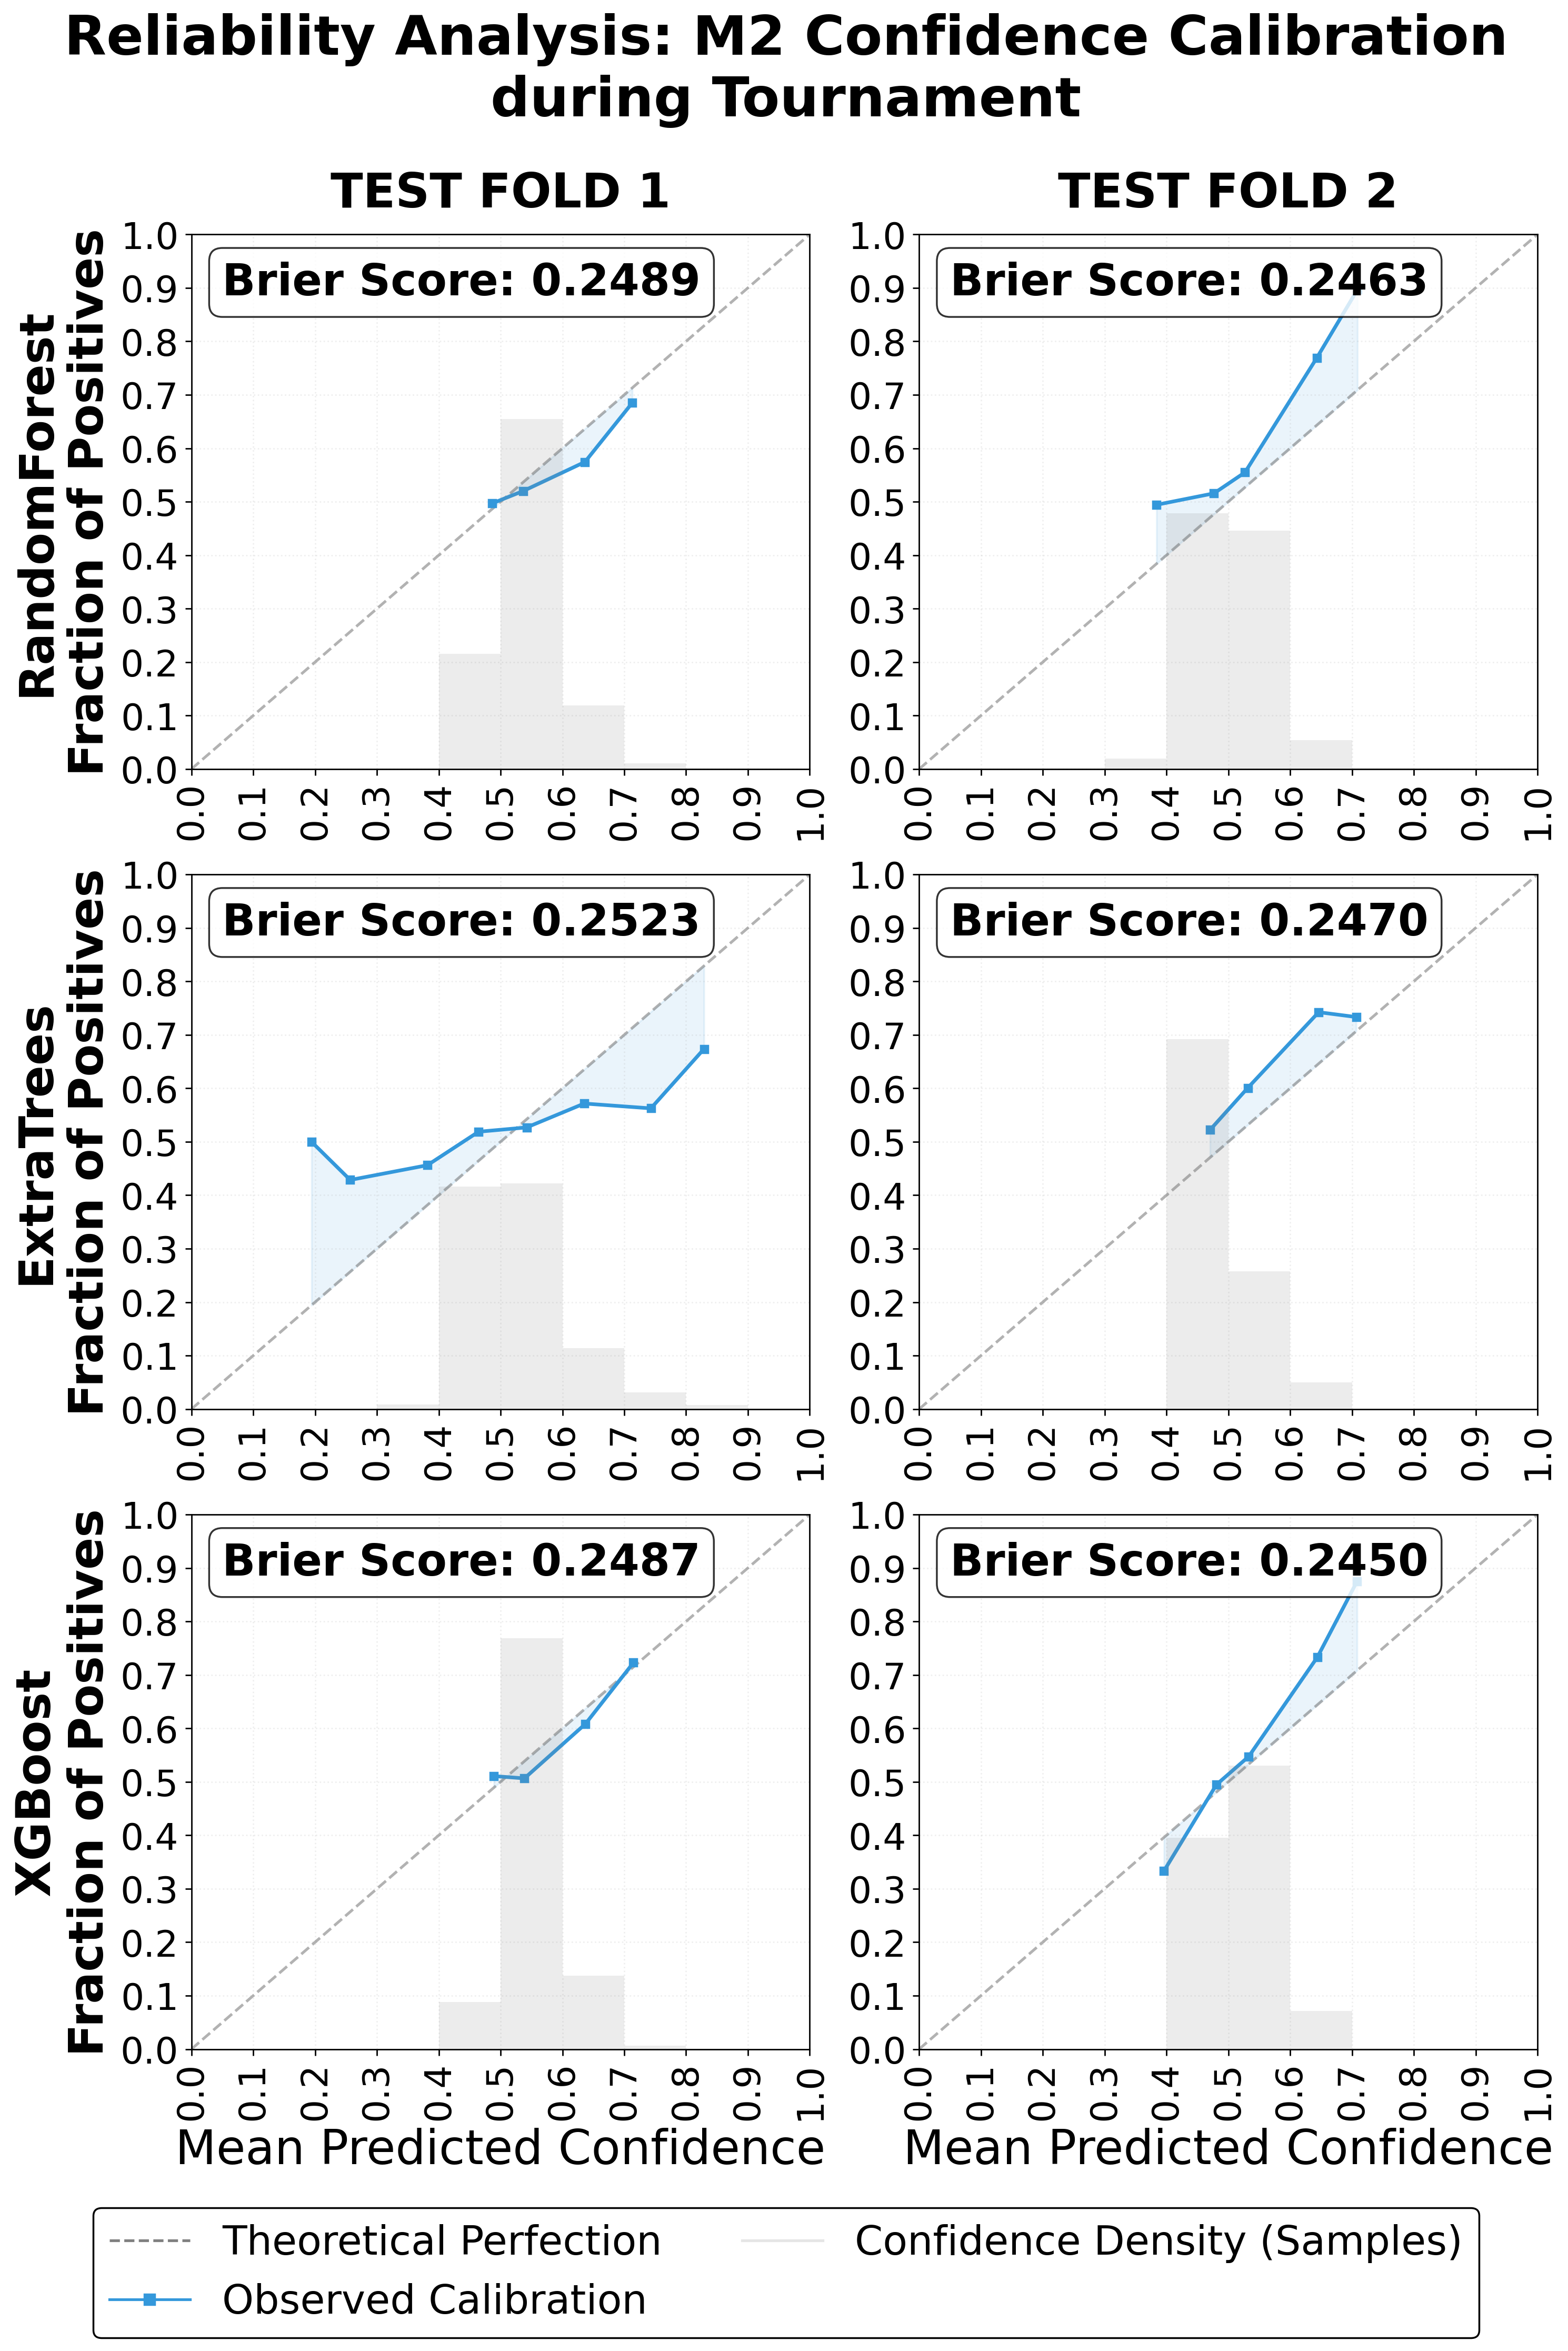
\includegraphics[width=\textwidth]{../data/figures/reliability_diagrams/Tournament_reliability_diagrams_part1.png}
        \caption{Model-Specific Reliability Diagrams During Tournament}
        \label{fig:model-specific reliability diagrams1}
    \end{minipage}
    \hfill
    \begin{minipage}[t]{0.49\textwidth}
        \centering
        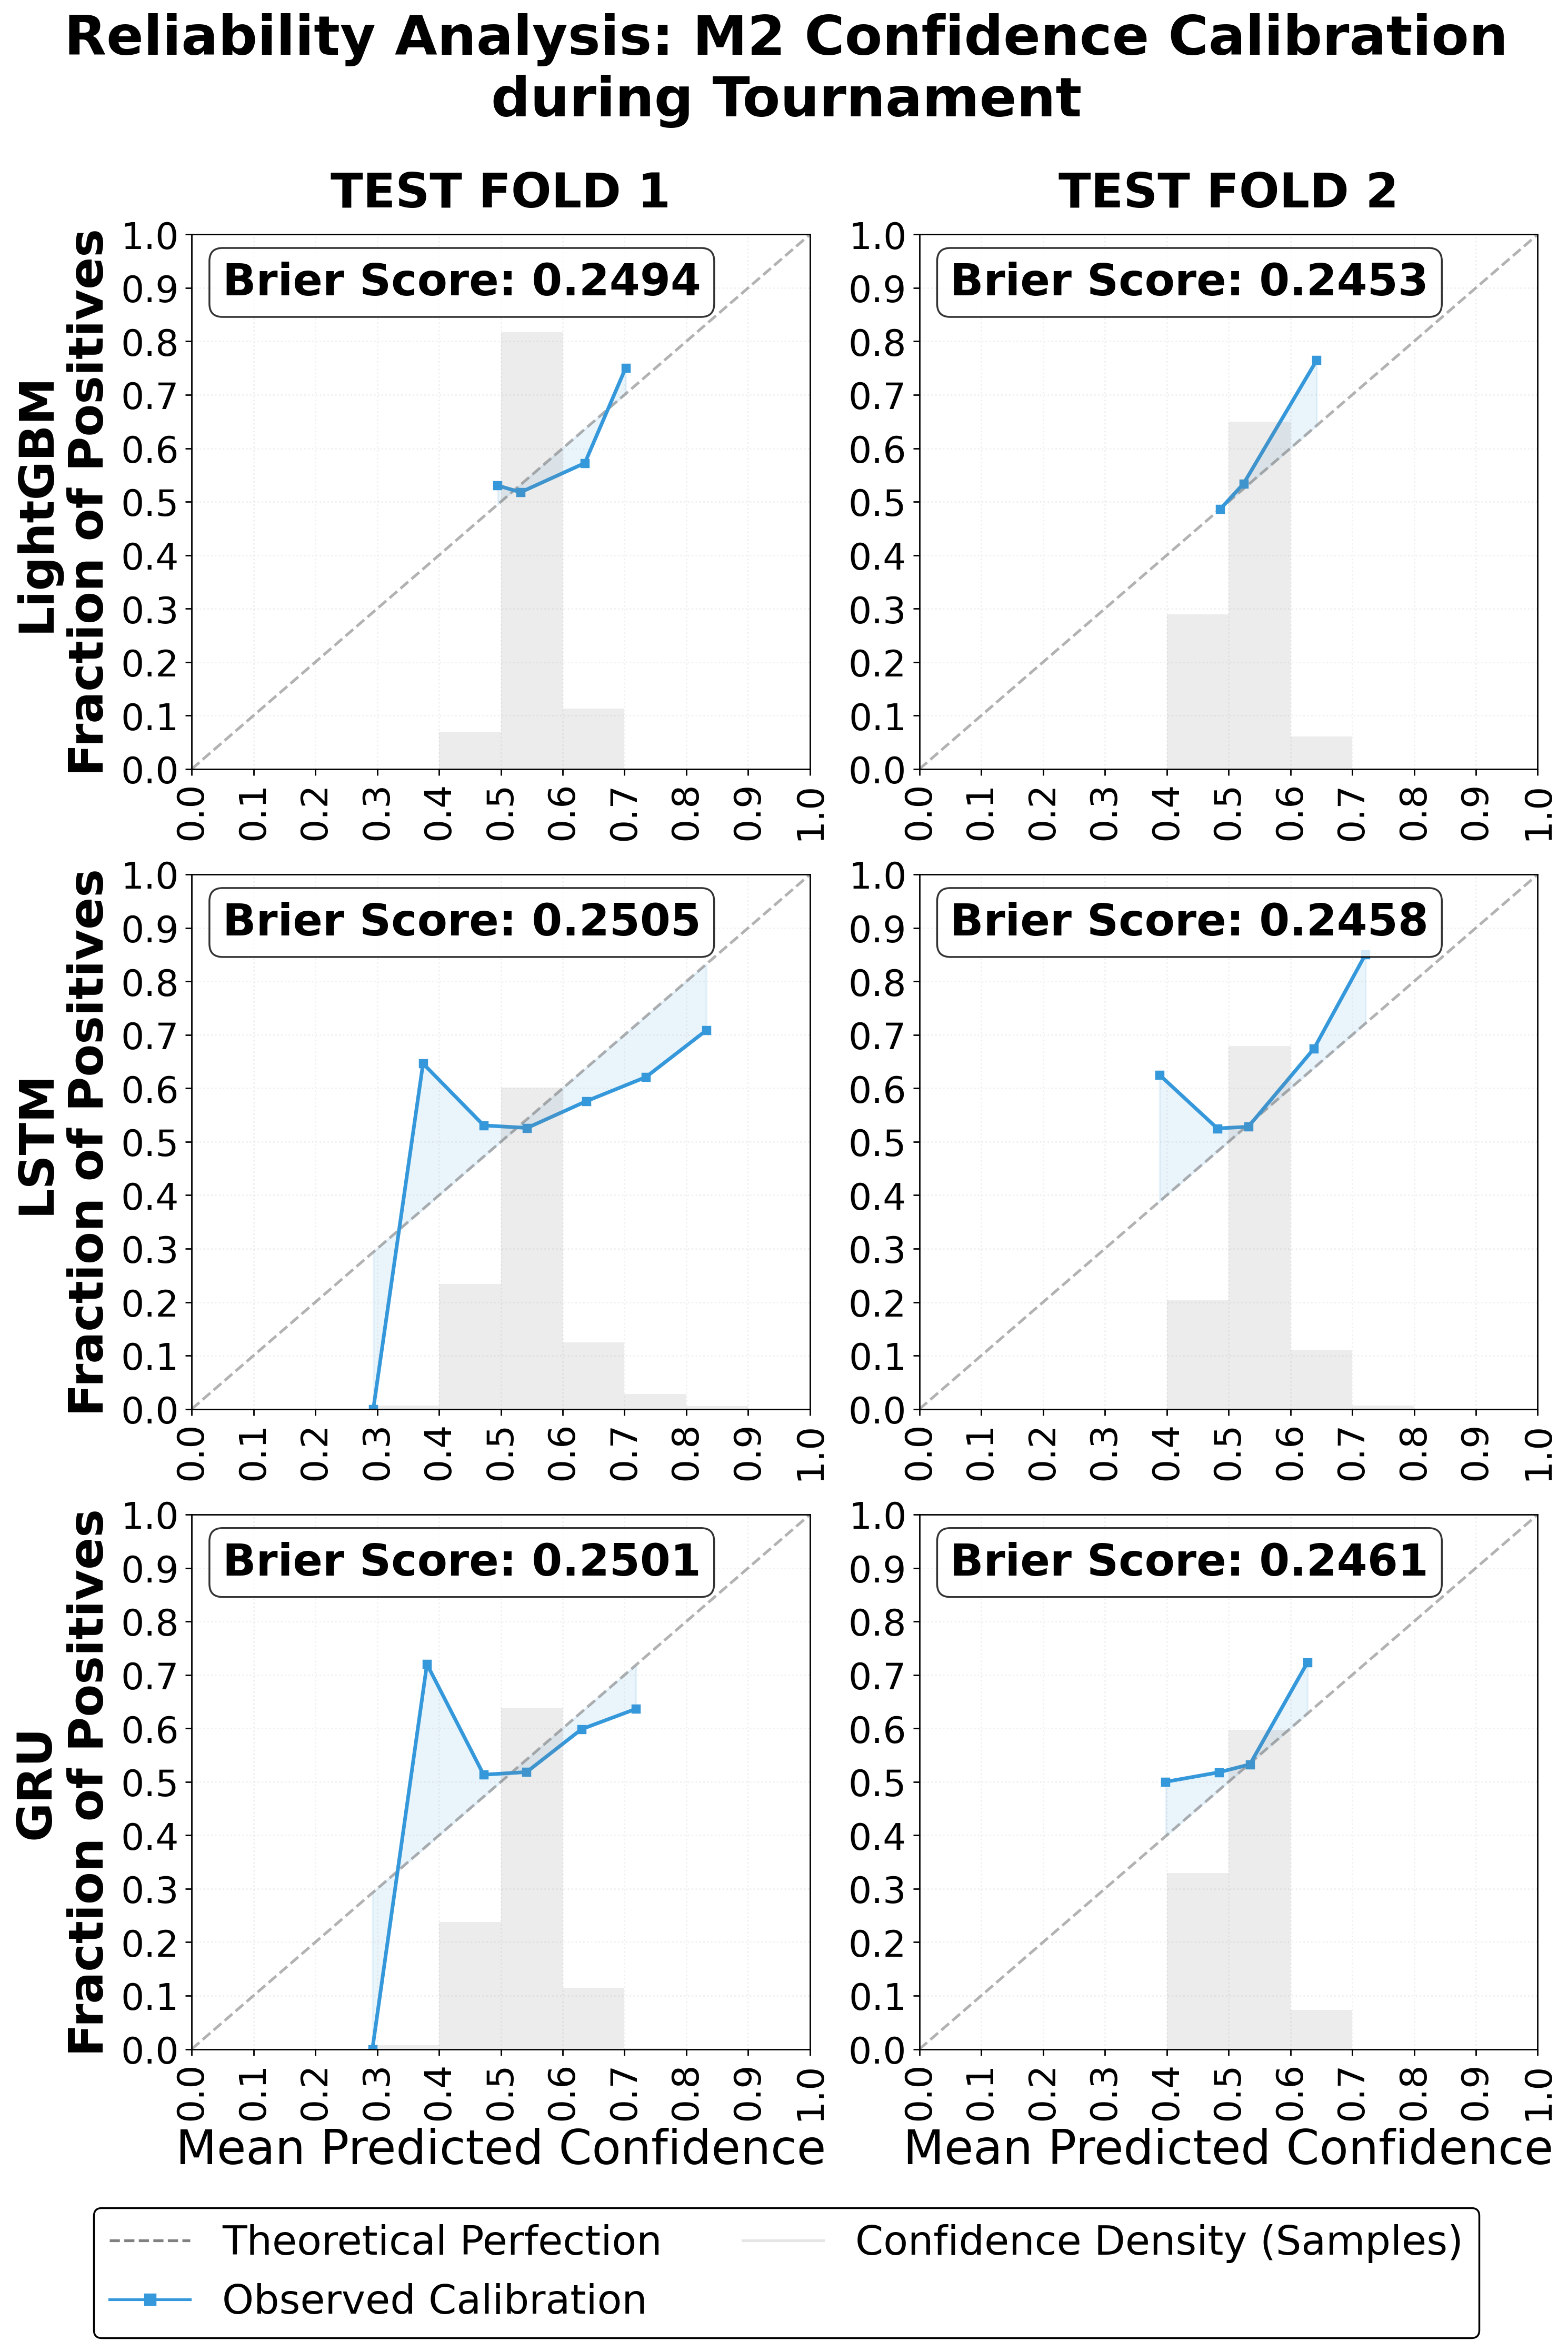
\includegraphics[width=\textwidth]{../data/figures/reliability_diagrams/Tournament_reliability_diagrams_part2.png}
        \caption{Model-Specific Reliability Diagrams During Tournament (Continued)}
        \label{fig:model-specific reliability diagrams2}
    \end{minipage}
\end{figure}

%%%%%%%%%%%%%%%%%%%%%%%%%%%%%%%%%%%%%%%%%%%%%%%%%%%%%%%%%%%%%%%%%%%%%%%%%%%%%%%%%%%%%%%%%%%%%%%%%%%%%%%%%%%%%%%%%%%%%%%%%%%
%%%%%%%%%%%%%%%%%%%%%%%%%%%%%%%%%%%%%%%%%%%%%%%%%%%%%%%%%%%%%%%%%%%%%%%%%%%%%%%%%%%%%%%%%%%%%%%%%%%%%%%%%%%%%%%%%%%%%%%%%%%
Lorem ipsum dolor sit amet, consectetur adipiscing elit. Sed do eiusmod tempor incididunt ut labore et dolore magna aliqua. 
Ut enim ad minim veniam, quis nostrud exercitation ullamco laboris nisi ut aliquip ex ea commodo consequat. 
Duis aute irure dolor in reprehenderit in voluptate velit esse cillum dolore eu fugiat nulla pariatur. 
Excepteur sint occaecat cupidatat non proident, sunt in culpa qui officia deserunt mollit anim id est laborum
Lorem ipsum dolor sit amet, consectetur adipiscing elit. Sed do eiusmod tempor incididunt ut labore et dolore magna aliqua. 
Ut enim ad minim veniam, quis nostrud exercitation ullamco laboris nisi ut aliquip ex ea commodo consequat. 
Duis aute irure dolor in reprehenderit in voluptate velit esse cillum dolore eu fugiat nulla pariatur. 
Excepteur sint occaecat cupidatat non proident, sunt in culpa qui officia deserunt mollit anim id est laborum
Lorem ipsum dolor sit amet, consectetur adipiscing elit. Sed do eiusmod tempor incididunt ut labore et dolore magna aliqua. 
Ut enim ad minim veniam, quis nostrud exercitation ullamco laboris nisi ut aliquip ex ea commodo consequat. 
Duis aute irure dolor in reprehenderit in voluptate velit esse cillum dolore eu fugiat nulla pariatur. 
Excepteur sint occaecat cupidatat non proident, sunt in culpa qui officia deserunt mollit anim id est laborum
%%%%%%%%%%%%%%%%%%%%%%%%%%%%%%%%%%%%%%%%%%%%%%%%%%%%%%%%%%%%%%%%%%%%%%%%%%%%%%%%%%%%%%%%%%%%%%%%%%%%%%%%%%%%%%%%%%%%%%%%%%%
%%%%%%%%%%%%%%%%%%%%%%%%%%%%%%%%%%%%%%%%%%%%%%%%%%%%%%%%%%%%%%%%%%%%%%%%%%%%%%%%%%%%%%%%%%%%%%%%%%%%%%%%%%%%%%%%%%%%%%%%%%%


\subsubsection{Tournament Evaluation}
\paragraph*{Overview}
This chapter presents the final results of the Architecture Tournament.
We evaluate model performance across backtests, analyze best- and worst-performing currency pairs, discuss model-specific limitations, and select the final architecture.

\paragraph{Model-Specific Backtest Performance and Aggregated Performance Ranking}
He expects you to argue:
"We propose a single model architecture for FX trading. For each currency pair, we tune a small set of interpretable parameters
(e.g., ATR multiplier, conformal threshold) that reflect that pair's unique volatility and liquidity characteristics.
This approach is robust: performance across 10 pairs shows average Sharpe 1.2 with standard deviation 0.2.
Majors outperform EMs as expected, but EMs remain profitable with adapted parameters."

\begin{figure}[H]
    \centering
    \begin{minipage}[t]{0.49\textwidth}
        \centering
        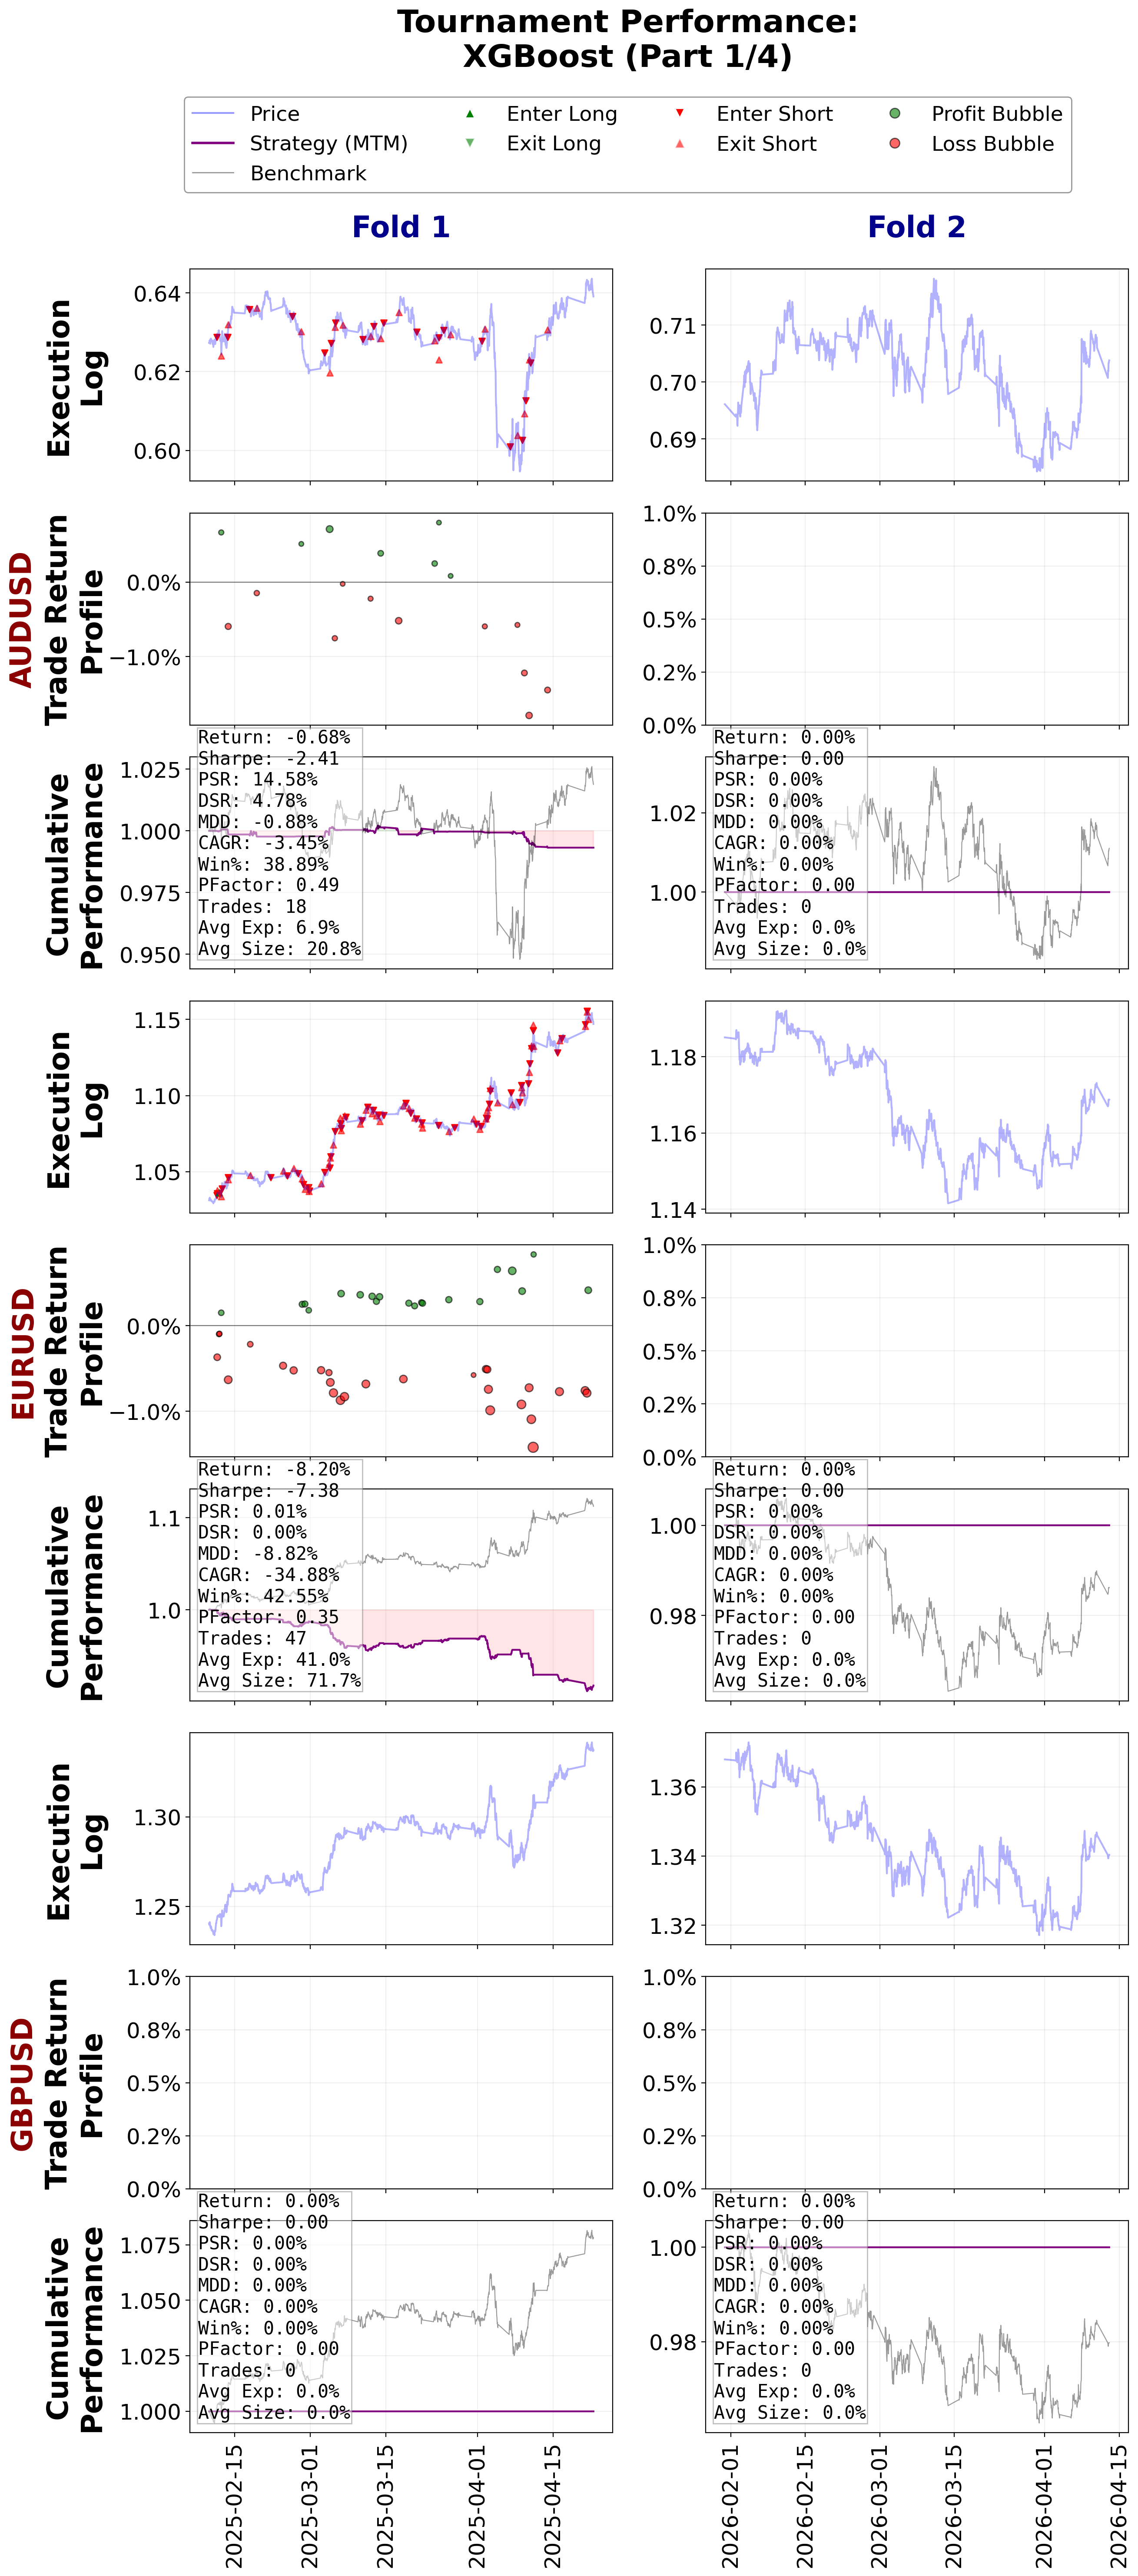
\includegraphics[width=\textwidth]{../data/figures/backtests/tournament_results_XGBoost_part1.png}
        \caption{Backtest Result of XGBoost During Tournament}
        \label{fig:tournament_results_XGBoost_1}
    \end{minipage}
    \hfill
    \begin{minipage}[t]{0.49\textwidth}
        \centering
        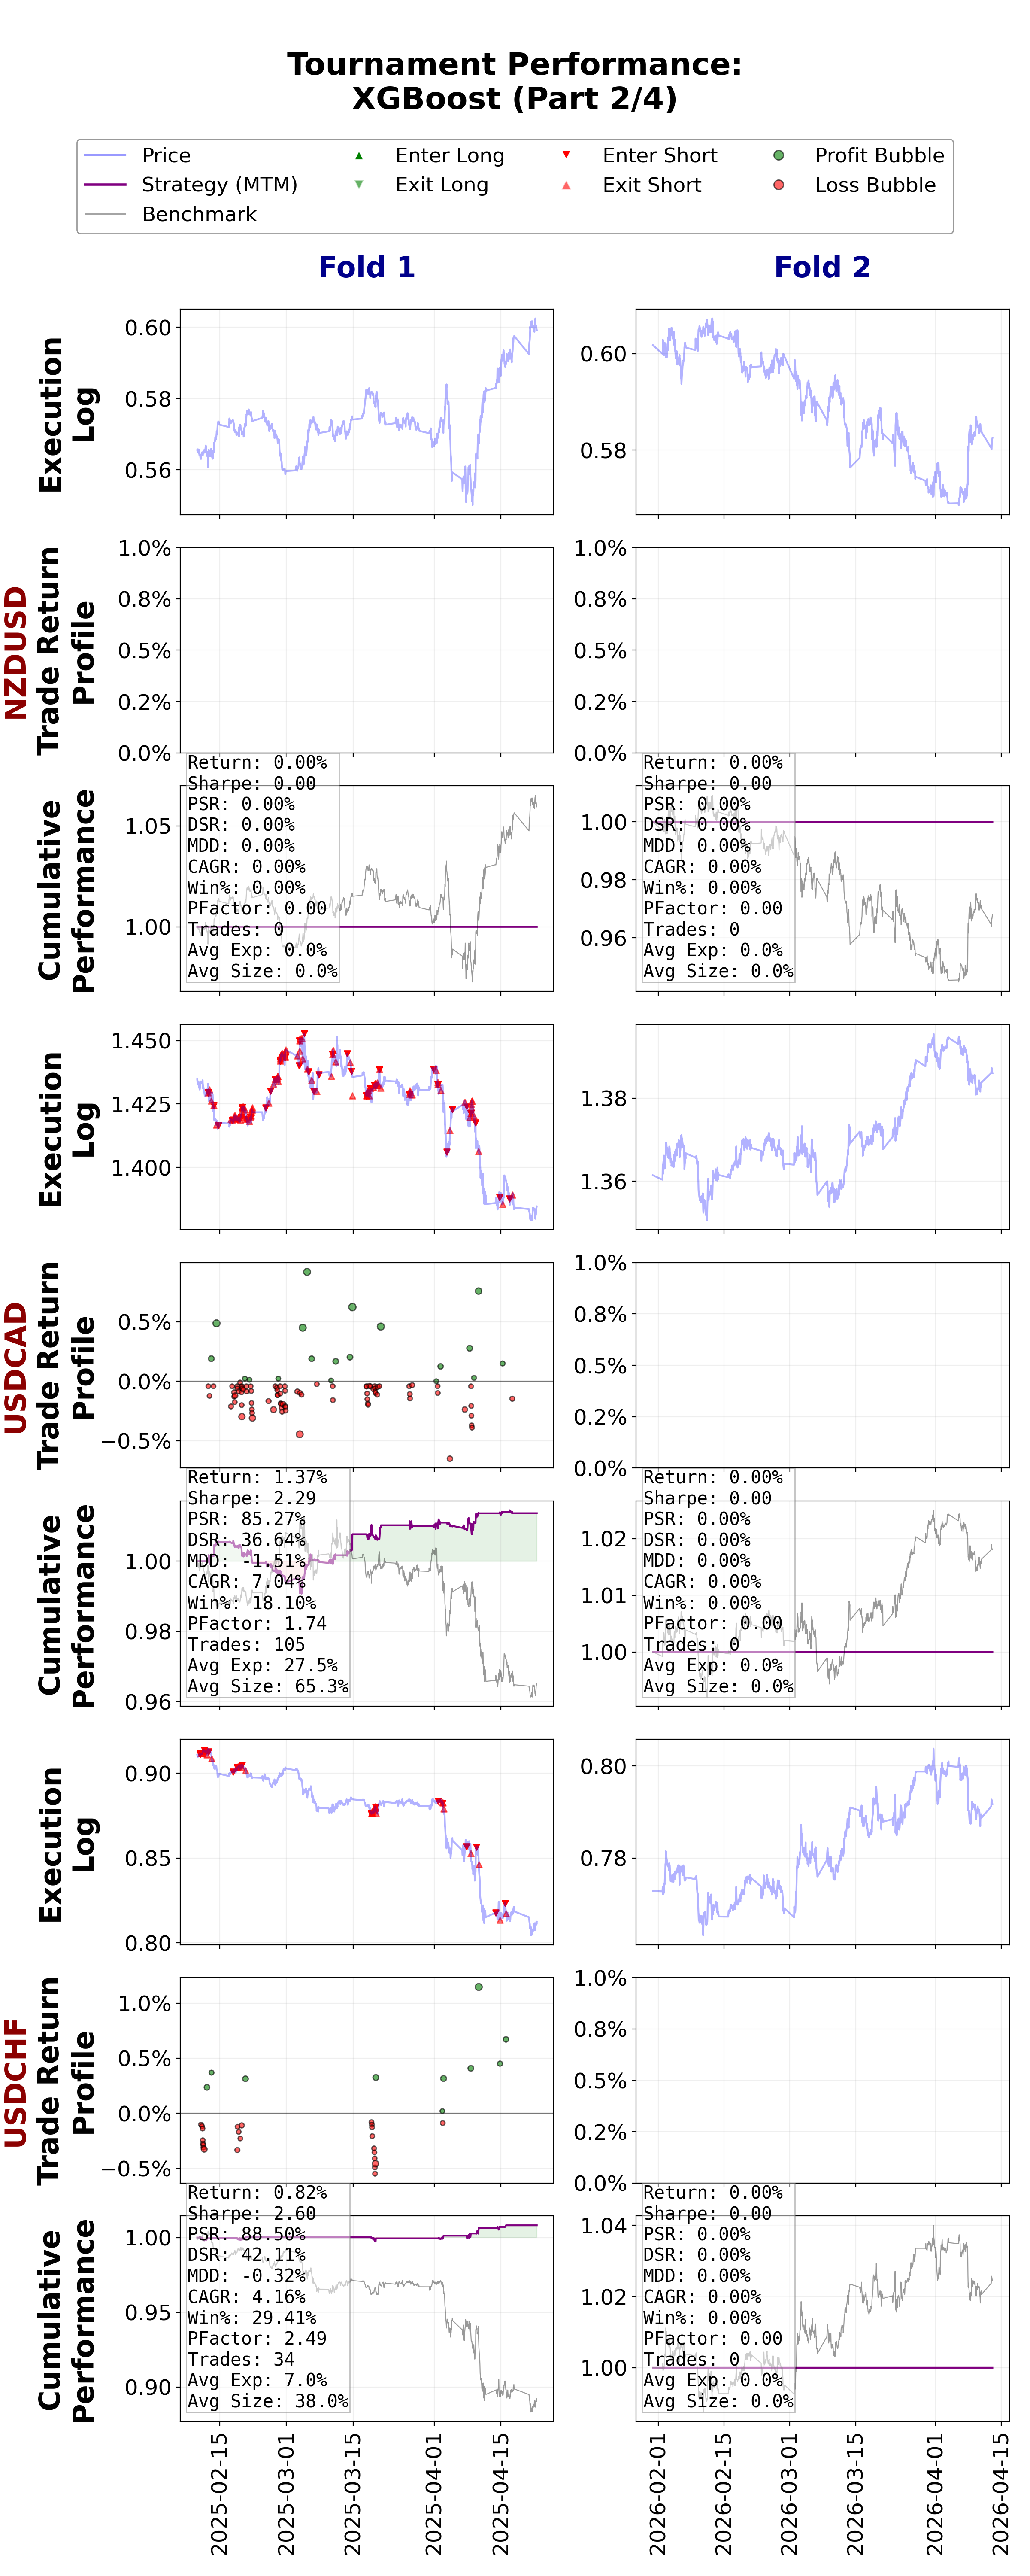
\includegraphics[width=\textwidth]{../data/figures/backtests/tournament_results_XGBoost_part2.png}
        \caption{Backtest Result of XGBoost During Tournament (Continued)}
        \label{fig:tournament_results_XGBoost_2}
    \end{minipage}
\end{figure}

\begin{figure}[H]
    \centering
    \begin{minipage}[t]{0.49\textwidth}
        \centering
        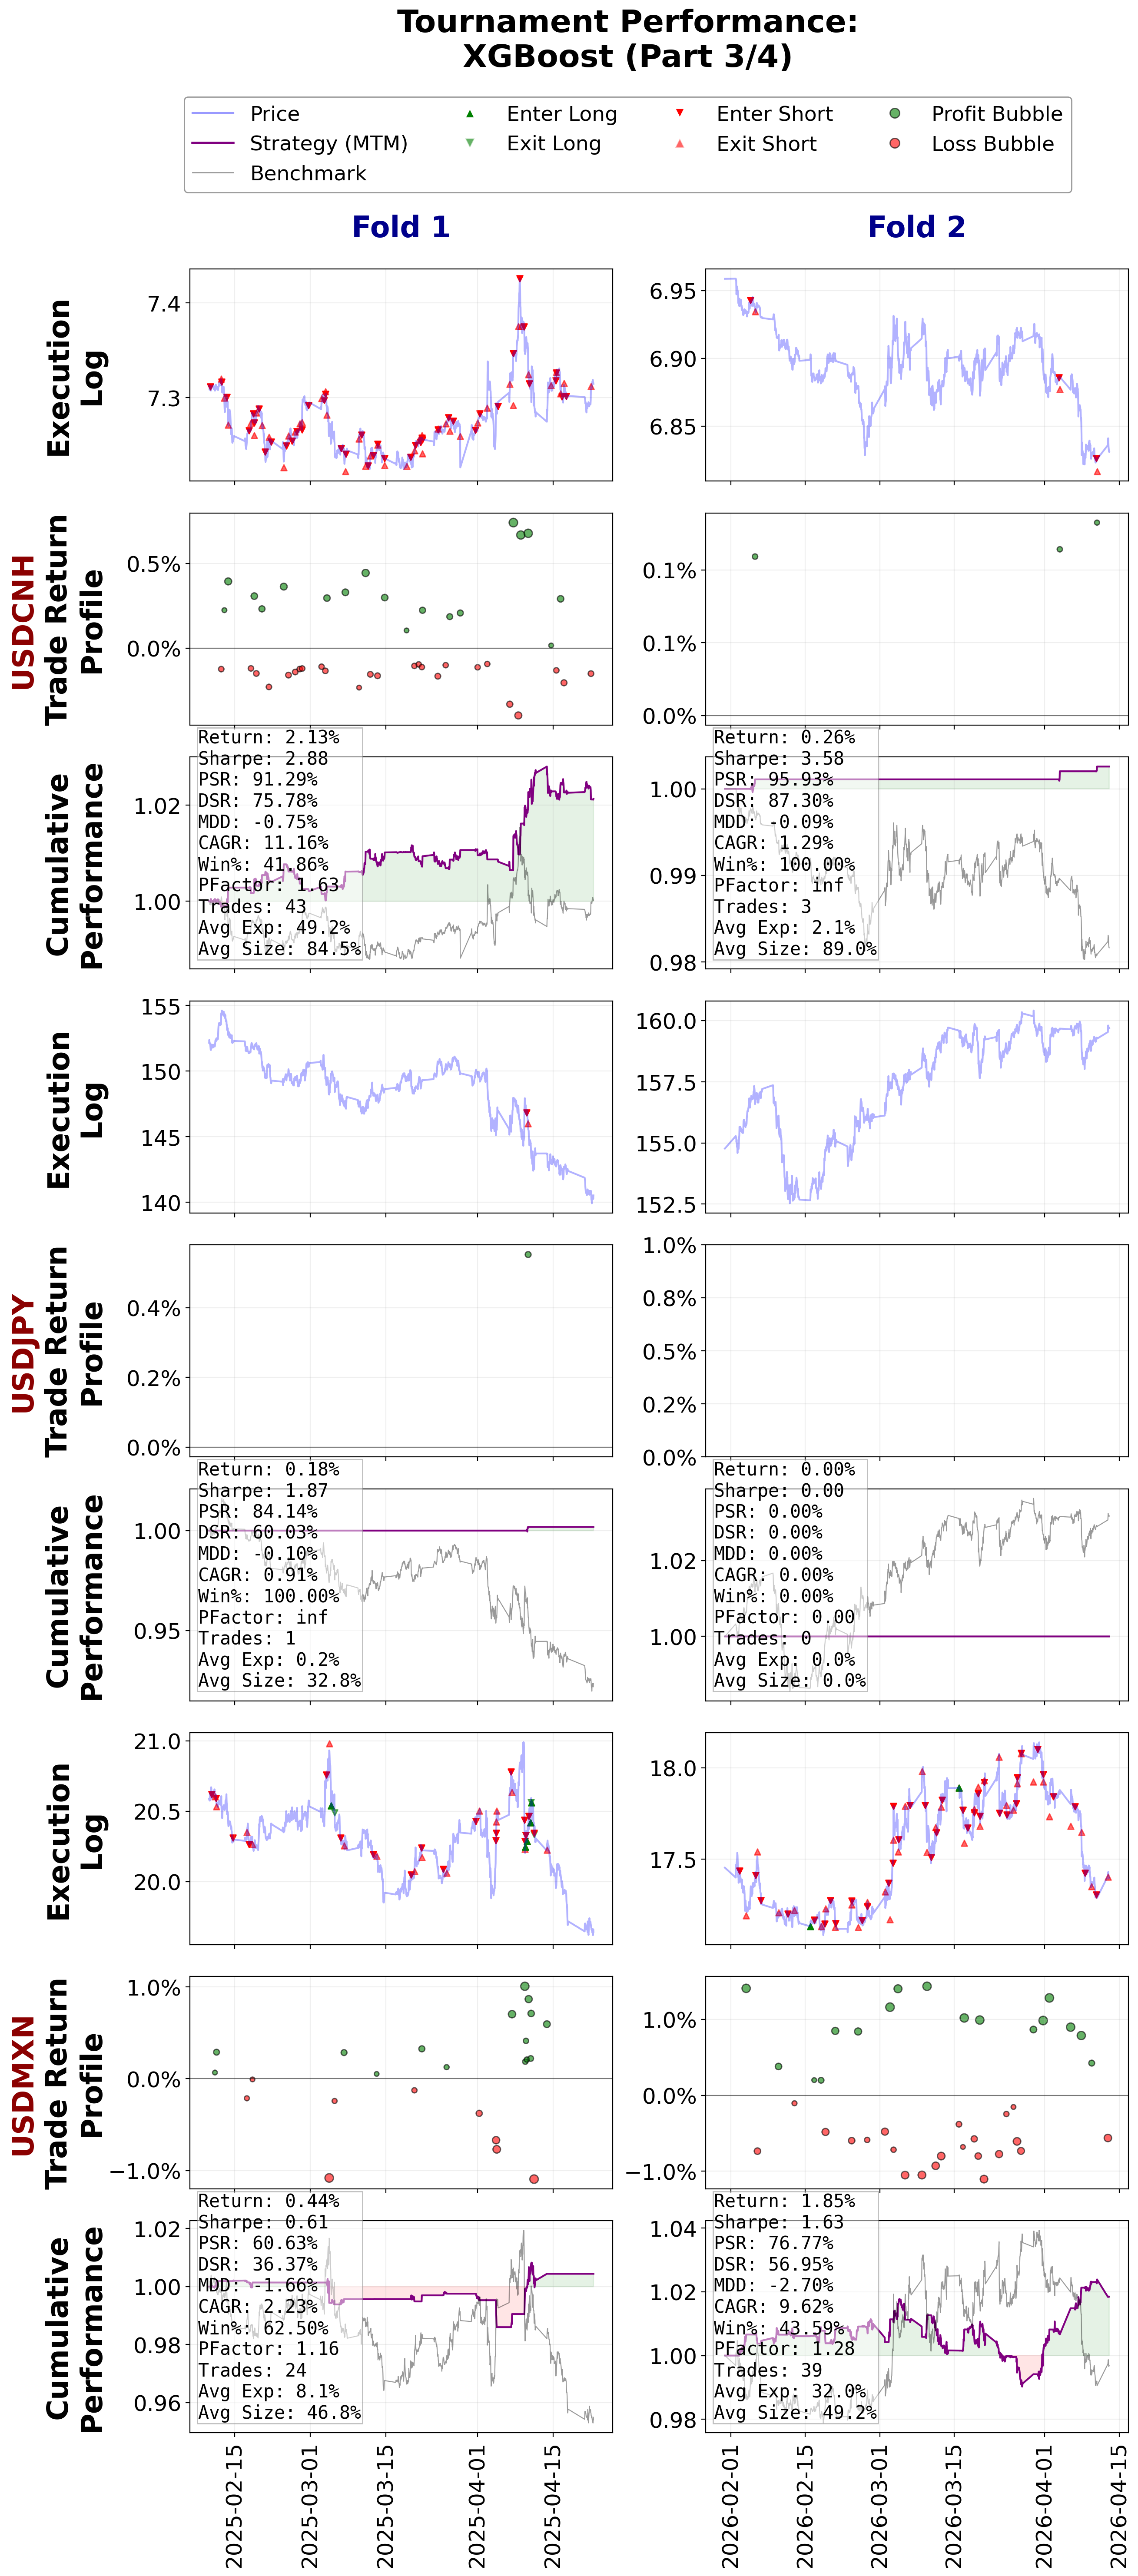
\includegraphics[width=\textwidth]{../data/figures/backtests/tournament_results_XGBoost_part3.png}
        \caption{Backtest Result of XGBoost During Tournament (Continued)}
        \label{fig:tournament_results_XGBoost_3}
    \end{minipage}
    \hfill
    \begin{minipage}[t]{0.49\textwidth}
        \centering
        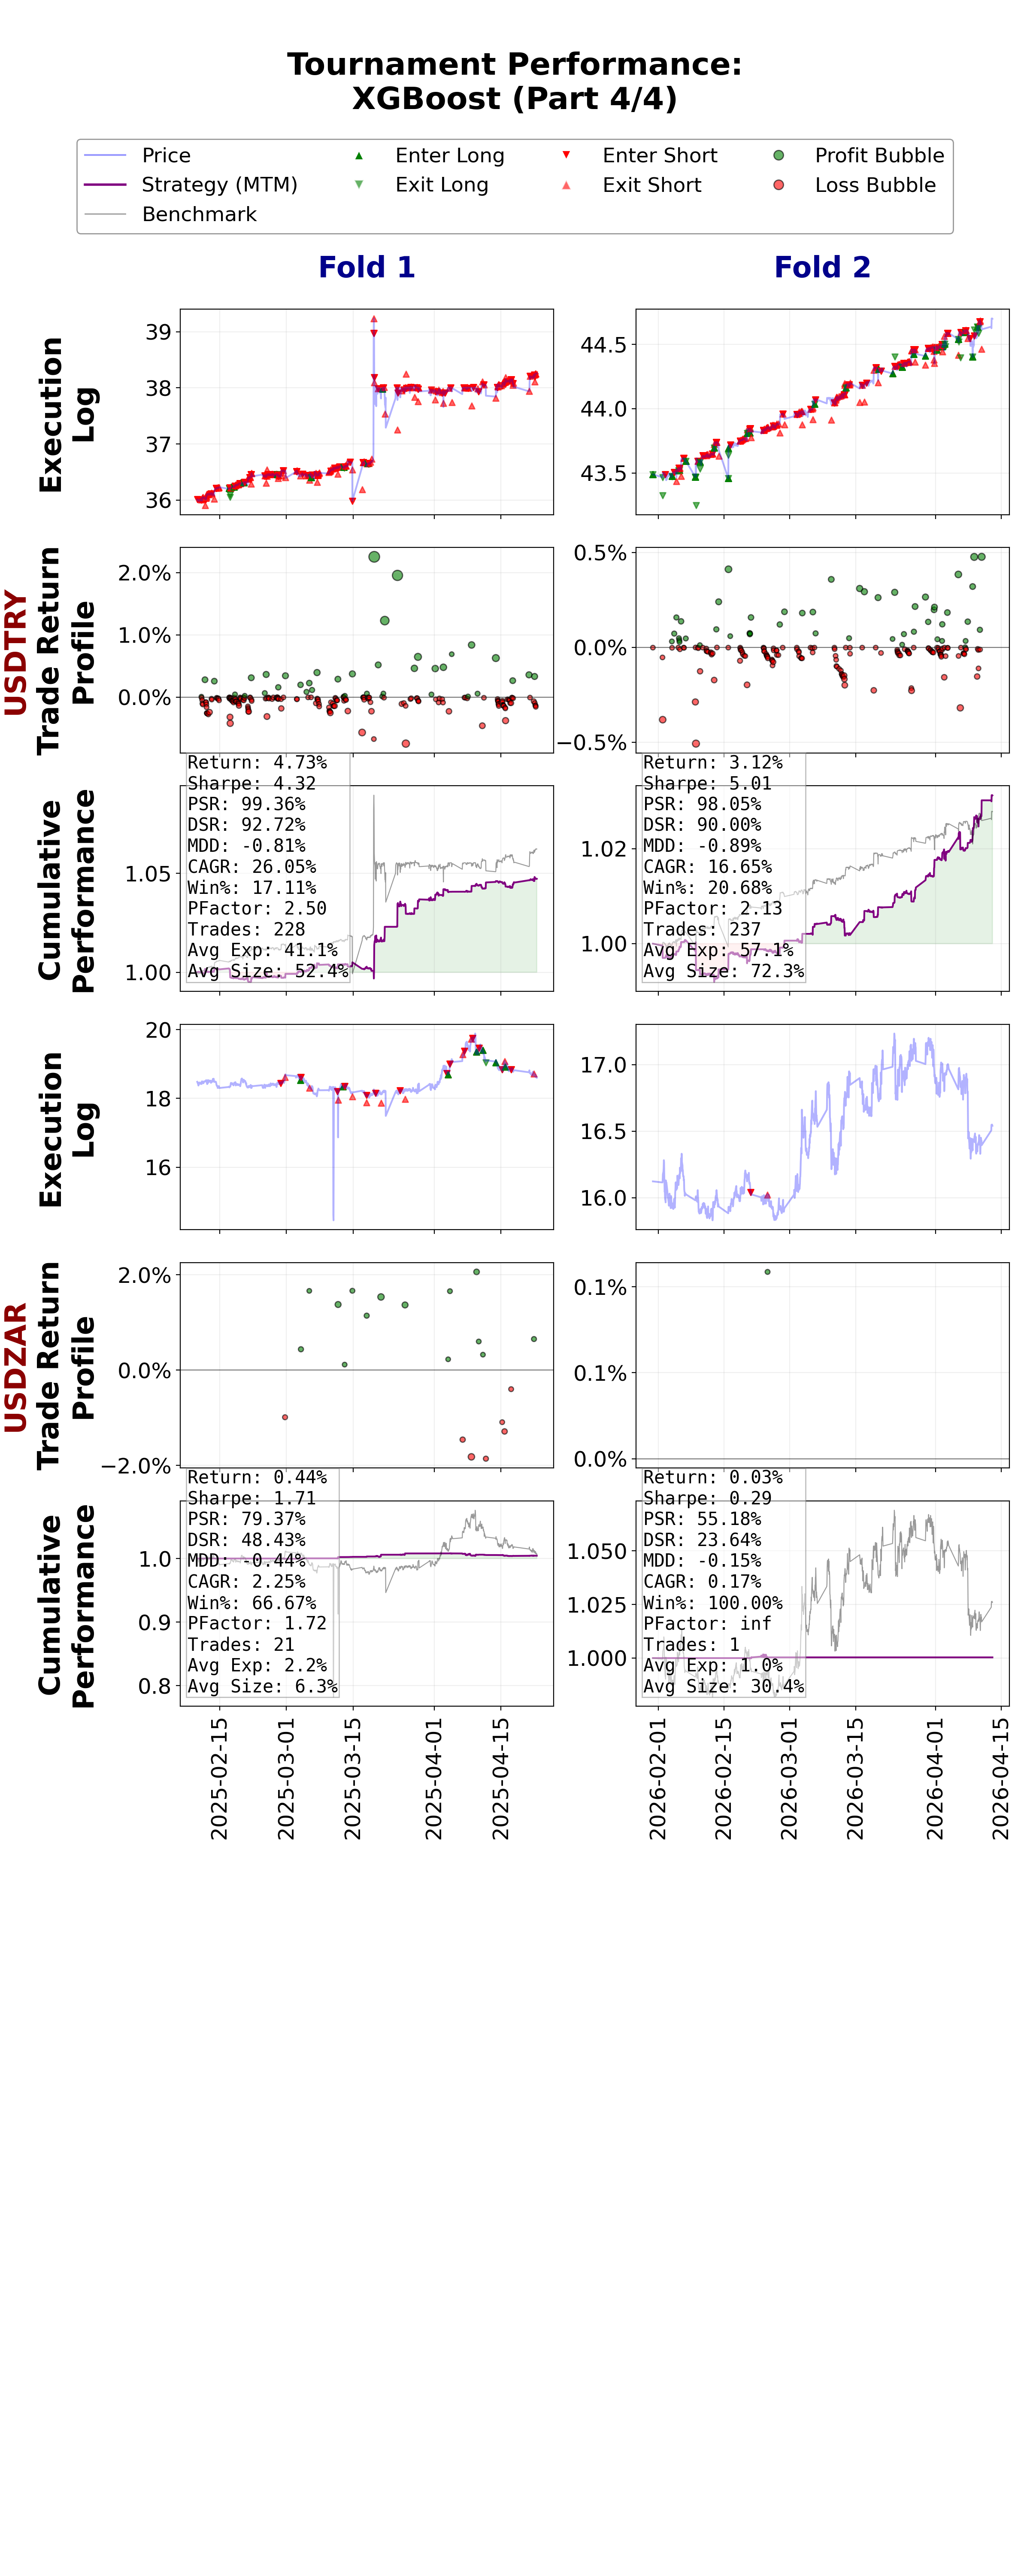
\includegraphics[width=\textwidth]{../data/figures/backtests/tournament_results_XGBoost_part4.png}
        \caption{Backtest Result of XGBoost During Tournament (Continued)}
        \label{fig:tournament_results_XGBoost_4}
    \end{minipage}
\end{figure}

%%%%%%%%%%%%%%%%%%%%%%%%%%%%%%%%%%%%%%%%%%%%%%%%%%%%%%%%%%%%%%%%%%%%%%%%%%%%%%%%%%%%%%%%%%%%%%%%%%%%%%%%%%%%%%%%%%%%%%%%%%%
%%%%%%%%%%%%%%%%%%%%%%%%%%%%%%%%%%%%%%%%%%%%%%%%%%%%%%%%%%%%%%%%%%%%%%%%%%%%%%%%%%%%%%%%%%%%%%%%%%%%%%%%%%%%%%%%%%%%%%%%%%%
Lorem ipsum dolor sit amet, consectetur adipiscing elit. Sed do eiusmod tempor incididunt ut labore et dolore magna aliqua. 
Ut enim ad minim veniam, quis nostrud exercitation ullamco laboris nisi ut aliquip ex ea commodo consequat. 
Duis aute irure dolor in reprehenderit in voluptate velit esse cillum dolore eu fugiat nulla pariatur. 
Excepteur sint occaecat cupidatat non proident, sunt in culpa qui officia deserunt mollit anim id est laborum
Lorem ipsum dolor sit amet, consectetur adipiscing elit. Sed do eiusmod tempor incididunt ut labore et dolore magna aliqua. 
Ut enim ad minim veniam, quis nostrud exercitation ullamco laboris nisi ut aliquip ex ea commodo consequat. 
Duis aute irure dolor in reprehenderit in voluptate velit esse cillum dolore eu fugiat nulla pariatur. 
Excepteur sint occaecat cupidatat non proident, sunt in culpa qui officia deserunt mollit anim id est laborum
Lorem ipsum dolor sit amet, consectetur adipiscing elit. Sed do eiusmod tempor incididunt ut labore et dolore magna aliqua. 
Ut enim ad minim veniam, quis nostrud exercitation ullamco laboris nisi ut aliquip ex ea commodo consequat. 
Duis aute irure dolor in reprehenderit in voluptate velit esse cillum dolore eu fugiat nulla pariatur. 
Excepteur sint occaecat cupidatat non proident, sunt in culpa qui officia deserunt mollit anim id est laborum
%%%%%%%%%%%%%%%%%%%%%%%%%%%%%%%%%%%%%%%%%%%%%%%%%%%%%%%%%%%%%%%%%%%%%%%%%%%%%%%%%%%%%%%%%%%%%%%%%%%%%%%%%%%%%%%%%%%%%%%%%%%
%%%%%%%%%%%%%%%%%%%%%%%%%%%%%%%%%%%%%%%%%%%%%%%%%%%%%%%%%%%%%%%%%%%%%%%%%%%%%%%%%%%%%%%%%%%%%%%%%%%%%%%%%%%%%%%%%%%%%%%%%%%

\begin{table}[H]
\centering
\caption{{Detailed Statistics by Model (Mean $\pm$ Std) - Tournament Phase}}
\label{tab:all_models_tournament}
\resizebox{\textwidth}{!}{\begin{tabular}{lllllll}
\toprule
Statistic & RandomForest & ExtraTrees & XGBoost & LightGBM & LSTM & GRU \\
\midrule
Total Return (\%) & $0.0173 \pm 0.0513$ & $0.0058 \pm 0.0178$ & $0.0180 \pm 0.0511$ & $0.0083 \pm 0.0199$ & $0.0030 \pm 0.0213$ & $0.0041 \pm 0.0250$ \\
Sharpe Ratio & $1.3700 \pm 4.2100$ & $0.9750 \pm 3.1924$ & $2.0741 \pm 4.9296$ & $1.3514 \pm 3.2258$ & $0.8373 \pm 3.2417$ & $0.3732 \pm 3.5449$ \\
Probabilistic Sharpe (\%) & $0.4464 \pm 0.4409$ & $0.3759 \pm 0.4095$ & $0.4537 \pm 0.4156$ & $0.4450 \pm 0.4345$ & $0.4009 \pm 0.4441$ & $0.3735 \pm 0.4206$ \\
Max Drawdown (\%) & $-0.0096 \pm 0.0131$ & $-0.0076 \pm 0.0095$ & $-0.0069 \pm 0.0081$ & $-0.0089 \pm 0.0135$ & $-0.0126 \pm 0.0154$ & $-0.0066 \pm 0.0106$ \\
CAGR (\%) & $0.1438 \pm 0.4479$ & $0.0378 \pm 0.1092$ & $0.1507 \pm 0.4916$ & $0.0526 \pm 0.1222$ & $0.0229 \pm 0.1294$ & $0.0322 \pm 0.1686$ \\
Win Rate (\%) & $0.3331 \pm 0.2699$ & $0.3569 \pm 0.3054$ & $0.3862 \pm 0.3123$ & $0.3126 \pm 0.3188$ & $0.3505 \pm 0.3123$ & $0.2826 \pm 0.3065$ \\
Profit Factor & $1.1805 \pm 1.3409$ & $0.8968 \pm 1.0099$ & $1.7786 \pm 2.7504$ & $inf \pm nan$ & $inf \pm nan$ & $1.2495 \pm 2.0817$ \\
Number of Trades & $41.8636 \pm 54.7586$ & $28.1818 \pm 30.8184$ & $32.6364 \pm 36.8931$ & $24.7273 \pm 34.7730$ & $29.0455 \pm 33.9390$ & $15.2727 \pm 21.4946$ \\
Avg Capital Exposure & $17.7691 \pm 17.7417$ & $16.9477 \pm 18.0934$ & $14.2541 \pm 14.4369$ & $15.0477 \pm 19.4399$ & $24.3782 \pm 26.0835$ & $11.1891 \pm 16.0362$ \\
Avg Trade Size & $30.8445 \pm 25.4981$ & $30.8164 \pm 28.0967$ & $33.4509 \pm 30.4589$ & $39.3268 \pm 34.1243$ & $38.8300 \pm 36.0490$ & $32.5464 \pm 32.3316$ \\
Deflated Sharpe & $0.3645 \pm 0.4057$ & $0.3072 \pm 0.3860$ & $0.3349 \pm 0.3721$ & $0.3657 \pm 0.3985$ & $0.3222 \pm 0.4000$ & $0.3010 \pm 0.3837$ \\
PFDR & $1.0000 \pm 0.0000$ & $1.0000 \pm 0.0000$ & $1.0000 \pm 0.0000$ & $1.0000 \pm 0.0000$ & $1.0000 \pm 0.0000$ & $1.0000 \pm 0.0000$ \\
M2 Brier & $0.2471 \pm 0.0017$ & $0.2471 \pm 0.0005$ & $0.2476 \pm 0.0022$ & $0.2468 \pm 0.0013$ & $0.2475 \pm 0.0000$ & $0.2485 \pm 0.0017$ \\
\bottomrule
\end{tabular}}
\end{table}


\begin{table}[H]
\centering
\caption{{Ranking Summary - Best Performer per Metric (Tournament Phase)}}
\label{tab:ranking_tournament}
\resizebox{\textwidth}{!}{\begin{tabular}{llll}
\toprule
Metric & Higher is Better & Best Model & Best Value \\
\midrule
Total Return (\%) & Yes & XGBoost & $0.0180$ \\
Sharpe Ratio & Yes & XGBoost & $2.0741$ \\
Probabilistic Sharpe (\%) & Yes & XGBoost & $0.4537$ \\
Max Drawdown (\%) & Yes & GRU & $-0.0066$ \\
CAGR (\%) & Yes & XGBoost & $0.1507$ \\
Win Rate (\%) & Yes & XGBoost & $0.3862$ \\
Profit Factor & Yes & LightGBM & $inf$ \\
Number of Trades & No & GRU & $15.2727$ \\
Avg Capital Exposure & No & GRU & $11.1891$ \\
Avg Trade Size & No & ExtraTrees & $30.8164$ \\
Deflated Sharpe & Yes & LightGBM & $0.3657$ \\
PFDR & No & RandomForest & $1.0000$ \\
M2 Brier & No & LightGBM & $0.2468$ \\
\\ \midrule \textbf{Overall RRF Winner} & & \textbf{XGBoost} & \textbf{Score: 0.2081} \\\bottomrule
\end{tabular}}
\end{table}


%%%%%%%%%%%%%%%%%%%%%%%%%%%%%%%%%%%%%%%%%%%%%%%%%%%%%%%%%%%%%%%%%%%%%%%%%%%%%%%%%%%%%%%%%%%%%%%%%%%%%%%%%%%%%%%%%%%%%%%%%%%
%%%%%%%%%%%%%%%%%%%%%%%%%%%%%%%%%%%%%%%%%%%%%%%%%%%%%%%%%%%%%%%%%%%%%%%%%%%%%%%%%%%%%%%%%%%%%%%%%%%%%%%%%%%%%%%%%%%%%%%%%%%
Lorem ipsum dolor sit amet, consectetur adipiscing elit. Sed do eiusmod tempor incididunt ut labore et dolore magna aliqua. 
Ut enim ad minim veniam, quis nostrud exercitation ullamco laboris nisi ut aliquip ex ea commodo consequat. 
Duis aute irure dolor in reprehenderit in voluptate velit esse cillum dolore eu fugiat nulla pariatur. 
Excepteur sint occaecat cupidatat non proident, sunt in culpa qui officia deserunt mollit anim id est laborum
Lorem ipsum dolor sit amet, consectetur adipiscing elit. Sed do eiusmod tempor incididunt ut labore et dolore magna aliqua. 
Ut enim ad minim veniam, quis nostrud exercitation ullamco laboris nisi ut aliquip ex ea commodo consequat. 
Duis aute irure dolor in reprehenderit in voluptate velit esse cillum dolore eu fugiat nulla pariatur. 
Excepteur sint occaecat cupidatat non proident, sunt in culpa qui officia deserunt mollit anim id est laborum
Lorem ipsum dolor sit amet, consectetur adipiscing elit. Sed do eiusmod tempor incididunt ut labore et dolore magna aliqua. 
Ut enim ad minim veniam, quis nostrud exercitation ullamco laboris nisi ut aliquip ex ea commodo consequat. 
Duis aute irure dolor in reprehenderit in voluptate velit esse cillum dolore eu fugiat nulla pariatur. 
Excepteur sint occaecat cupidatat non proident, sunt in culpa qui officia deserunt mollit anim id est laborum
%%%%%%%%%%%%%%%%%%%%%%%%%%%%%%%%%%%%%%%%%%%%%%%%%%%%%%%%%%%%%%%%%%%%%%%%%%%%%%%%%%%%%%%%%%%%%%%%%%%%%%%%%%%%%%%%%%%%%%%%%%%
%%%%%%%%%%%%%%%%%%%%%%%%%%%%%%%%%%%%%%%%%%%%%%%%%%%%%%%%%%%%%%%%%%%%%%%%%%%%%%%%%%%%%%%%%%%%%%%%%%%%%%%%%%%%%%%%%%%%%%%%%%%


\paragraph{Granular Performance Analysis and Best- and Worst-Performing Pairs per Model}

is it because model failed? Is it because pair is untradeable? Answer questions
Is it a data issue? Ie gaps overnight? More missing data than other pairs?
Is the model fundamentally weong dor that regime?

\begin{table}[H] \centering
\caption{RRF Granular Rankings (Tournament Phase)}
\label{tab:rrf_matrix_tournament}
\small \begin{tabular}{l l cccccc}
\toprule
Currency Pair & Fold & \rotatebox{90}{RandomForest} & \rotatebox{90}{ExtraTrees} & \rotatebox{90}{XGBoost} & \rotatebox{90}{LightGBM} & \rotatebox{90}{LSTM} & \rotatebox{90}{GRU} \\
\midrule
AUDUSD & Fold 1 & 6 (0.121) & 5 (0.121) & 9 (0.117) & 5 (0.123) & 11 (0.116) & 9 (0.119) \\
 & Fold 2 & 6 (0.122) & 4 (0.125) & 6 (0.122) & 4 (0.124) & 3 (0.126) & 5 (0.122) \\
EURUSD & Fold 1 & 8 (0.119) & 9 (0.120) & 11 (0.114) & 6 (0.122) & 9 (0.118) & 11 (0.116) \\
 & Fold 2 & 6 (0.122) & 11 (0.119) & 6 (0.122) & 4 (0.124) & 11 (0.120) & 5 (0.122) \\
GBPUSD & Fold 1 & 7 (0.119) & 11 (0.116) & 10 (0.116) & 11 (0.113) & 10 (0.116) & 5 (0.121) \\
 & Fold 2 & 4 (0.125) & 4 (0.125) & 6 (0.122) & 4 (0.124) & 3 (0.126) & 5 (0.122) \\
NZDUSD & Fold 1 & 5 (0.123) & 5 (0.121) & 7 (0.119) & 8 (0.118) & 8 (0.118) & 10 (0.117) \\
 & Fold 2 & 6 (0.122) & 4 (0.125) & 5 (0.125) & 9 (0.120) & 3 (0.126) & 3 (0.126) \\
USDCAD & Fold 1 & 8 (0.119) & 10 (0.117) & 5 (0.123) & 7 (0.120) & 4 (0.123) & 8 (0.119) \\
 & Fold 2 & 6 (0.122) & 4 (0.125) & 4 (0.126) & 4 (0.124) & 3 (0.126) & 5 (0.122) \\
USDCHF & Fold 1 & 10 (0.117) & 4 (0.126) & 2 (0.128) & 10 (0.114) & 1 (0.128) & 6 (0.121) \\
 & Fold 2 & 6 (0.122) & 4 (0.125) & 6 (0.122) & 10 (0.120) & 2 (0.128) & 5 (0.122) \\
USDCNH & Fold 1 & 3 (0.125) & 5 (0.121) & 3 (0.128) & 2 (0.127) & 5 (0.123) & 4 (0.125) \\
 & Fold 2 & 3 (0.125) & 4 (0.125) & 2 (0.127) & 2 (0.128) & 1 (0.129) & 10 (0.120) \\
USDJPY & Fold 1 & 11 (0.116) & 3 (0.126) & 8 (0.118) & 9 (0.118) & 7 (0.119) & 6 (0.121) \\
 & Fold 2 & 6 (0.122) & 4 (0.125) & 6 (0.122) & 11 (0.118) & 3 (0.126) & 11 (0.118) \\
USDMXN & Fold 1 & 4 (0.125) & 5 (0.121) & 6 (0.122) & 3 (0.126) & 6 (0.121) & 3 (0.126) \\
 & Fold 2 & 5 (0.124) & 1 (0.128) & 11 (0.118) & 3 (0.126) & 10 (0.122) & 4 (0.124) \\
USDTRY & Fold 1 & 1 (0.128) & 1 (0.129) & 1 (0.128) & 1 (0.130) & 3 (0.127) & 1 (0.129) \\
 & Fold 2 & 1 (0.128) & 2 (0.127) & 3 (0.127) & 4 (0.124) & 3 (0.126) & 1 (0.128) \\
USDZAR & Fold 1 & 2 (0.127) & 2 (0.127) & 4 (0.124) & 4 (0.125) & 2 (0.128) & 2 (0.127) \\
 & Fold 2 & 2 (0.127) & 3 (0.126) & 1 (0.129) & 1 (0.128) & 3 (0.126) & 2 (0.127) \\
\bottomrule
\end{tabular}
\end{table}


\begin{table}[H]
\caption{RRF Performance Summary: Best and Worst Performing Pairs (Tournament Phase)}
\label{tab:rrf_summary_tournament}
\begin{tabular}{l l p{5cm} p{5cm}}
\toprule
Model & Fold & Best Performers (RRF) & Worst Performers (RRF) \\
\midrule
RandomForest & Fold 1 & USDTRY, USDCNH & NZDUSD, AUDUSD \\
 & Fold 2 & USDTRY, EURUSD & USDMXN, USDZAR \\
ExtraTrees & Fold 1 & USDTRY, USDJPY & NZDUSD, GBPUSD \\
 & Fold 2 & USDTRY, USDZAR & USDCNH, USDMXN \\
XGBoost & Fold 1 & USDTRY, USDZAR & EURUSD, AUDUSD \\
 & Fold 2 & USDTRY, USDZAR & USDMXN, USDJPY \\
LightGBM & Fold 1 & USDTRY, USDCAD & NZDUSD, GBPUSD \\
 & Fold 2 & USDTRY, USDMXN & USDCNH, USDZAR \\
LSTM & Fold 1 & USDCHF, USDTRY & AUDUSD, NZDUSD \\
 & Fold 2 & USDTRY, USDCNH & USDMXN, USDJPY \\
GRU & Fold 1 & USDMXN, USDTRY & EURUSD, GBPUSD \\
 & Fold 2 & USDTRY, USDCNH & USDZAR, USDJPY \\
\bottomrule
\end{tabular}
\end{table}


%%%%%%%%%%%%%%%%%%%%%%%%%%%%%%%%%%%%%%%%%%%%%%%%%%%%%%%%%%%%%%%%%%%%%%%%%%%%%%%%%%%%%%%%%%%%%%%%%%%%%%%%%%%%%%%%%%%%%%%%%%%
%%%%%%%%%%%%%%%%%%%%%%%%%%%%%%%%%%%%%%%%%%%%%%%%%%%%%%%%%%%%%%%%%%%%%%%%%%%%%%%%%%%%%%%%%%%%%%%%%%%%%%%%%%%%%%%%%%%%%%%%%%%
Lorem ipsum dolor sit amet, consectetur adipiscing elit. Sed do eiusmod tempor incididunt ut labore et dolore magna aliqua. 
Ut enim ad minim veniam, quis nostrud exercitation ullamco laboris nisi ut aliquip ex ea commodo consequat. 
Duis aute irure dolor in reprehenderit in voluptate velit esse cillum dolore eu fugiat nulla pariatur. 
Excepteur sint occaecat cupidatat non proident, sunt in culpa qui officia deserunt mollit anim id est laborum
Lorem ipsum dolor sit amet, consectetur adipiscing elit. Sed do eiusmod tempor incididunt ut labore et dolore magna aliqua. 
Ut enim ad minim veniam, quis nostrud exercitation ullamco laboris nisi ut aliquip ex ea commodo consequat. 
Duis aute irure dolor in reprehenderit in voluptate velit esse cillum dolore eu fugiat nulla pariatur. 
Excepteur sint occaecat cupidatat non proident, sunt in culpa qui officia deserunt mollit anim id est laborum
Lorem ipsum dolor sit amet, consectetur adipiscing elit. Sed do eiusmod tempor incididunt ut labore et dolore magna aliqua. 
Ut enim ad minim veniam, quis nostrud exercitation ullamco laboris nisi ut aliquip ex ea commodo consequat. 
Duis aute irure dolor in reprehenderit in voluptate velit esse cillum dolore eu fugiat nulla pariatur. 
Excepteur sint occaecat cupidatat non proident, sunt in culpa qui officia deserunt mollit anim id est laborum
%%%%%%%%%%%%%%%%%%%%%%%%%%%%%%%%%%%%%%%%%%%%%%%%%%%%%%%%%%%%%%%%%%%%%%%%%%%%%%%%%%%%%%%%%%%%%%%%%%%%%%%%%%%%%%%%%%%%%%%%%%%
%%%%%%%%%%%%%%%%%%%%%%%%%%%%%%%%%%%%%%%%%%%%%%%%%%%%%%%%%%%%%%%%%%%%%%%%%%%%%%%%%%%%%%%%%%%%%%%%%%%%%%%%%%%%%%%%%%%%%%%%%%%

\begin{table}[H]
\centering
\caption{{Granular Performance Analysis XGBoost (Tournament Phase)}}
\label{tab:perf_XGBoost_tournament}
\resizebox{\textwidth}{!}{\begin{tabular}{rrrrrrrrrrrrrr}
\toprule
Pair & Fold & \rotatebox{90}{Total Return (\%)} & \rotatebox{90}{Sharpe Ratio} & \rotatebox{90}{Probabilistic Sharpe (\%)} & \rotatebox{90}{Max Drawdown (\%)} & \rotatebox{90}{CAGR (\%)} & \rotatebox{90}{Win Rate (\%)} & \rotatebox{90}{Profit Factor} & \rotatebox{90}{Number of Trades} & \rotatebox{90}{Avg Capital Exposure (\%)} & \rotatebox{90}{Avg Trade Size (\%)} & \rotatebox{90}{Deflated Sharpe (\%)} & \rotatebox{90}{M2 Brier} \\
\midrule
AUDUSD & Fold 1 & -0.68\% & -2.41 & 14.58\% & -0.88\% & -3.45\% & 38.89\% & 0.49 & 18.00 & 6.92\% & 20.76\% & 4.78\% & 0.25 \\
 & Fold 2 & 0.0000\% & 0.0000 & 0.0000\% & 0.0000\% & 0.0000\% & 0.0000\% & 0.0000 & 0.0000 & 0.0000\% & 0.0000\% & 0.0000\% & 0.25 \\
EURUSD & Fold 1 & -8.20\% & -7.38 & 0.01\% & -8.82\% & -34.88\% & 42.55\% & 0.35 & 47.00 & 41.00\% & 71.72\% & 0.0000\% & 0.25 \\
 & Fold 2 & 0.0000\% & 0.0000 & 0.0000\% & 0.0000\% & 0.0000\% & 0.0000\% & 0.0000 & 0.0000 & 0.0000\% & 0.0000\% & 0.0000\% & 0.25 \\
GBPUSD & Fold 1 & 0.0000\% & 0.0000 & 0.0000\% & 0.0000\% & 0.0000\% & 0.0000\% & 0.0000 & 0.0000 & 0.0000\% & 0.0000\% & 0.0000\% & 0.25 \\
 & Fold 2 & 0.0000\% & 0.0000 & 0.0000\% & 0.0000\% & 0.0000\% & 0.0000\% & 0.0000 & 0.0000 & 0.0000\% & 0.0000\% & 0.0000\% & 0.25 \\
NZDUSD & Fold 1 & -0.89\% & -1.40 & 26.83\% & -2.03\% & -4.38\% & 58.33\% & 0.66 & 12.00 & 14.87\% & 61.48\% & 10.85\% & 0.25 \\
 & Fold 2 & 0.0000\% & 0.0000 & 0.0000\% & 0.0000\% & 0.0000\% & 0.0000\% & 0.0000 & 0.0000 & 0.0000\% & 0.0000\% & 0.0000\% & 0.25 \\
USDCAD & Fold 1 & 0.11\% & 0.42 & 57.40\% & -0.58\% & 0.55\% & 37.50\% & 1.15 & 8.00 & 5.40\% & 34.84\% & 33.20\% & 0.25 \\
 & Fold 2 & 0.0000\% & 0.0000 & 0.0000\% & 0.0000\% & 0.0000\% & 0.0000\% & 0.0000 & 0.0000 & 0.0000\% & 0.0000\% & 0.0000\% & 0.25 \\
USDCHF & Fold 1 & -0.38\% & -1.80 & 19.30\% & -0.54\% & -1.88\% & 33.33\% & 0.50 & 6.00 & 3.74\% & 60.15\% & 6.19\% & 0.25 \\
 & Fold 2 & 0.0000\% & 0.0000 & 0.0000\% & 0.0000\% & 0.0000\% & 0.0000\% & 0.0000 & 0.0000 & 0.0000\% & 0.0000\% & 0.0000\% & 0.25 \\
USDCNH & Fold 1 & 2.13\% & 2.88 & 91.29\% & -0.75\% & 11.16\% & 41.86\% & 1.63 & 43.00 & 49.23\% & 84.45\% & 75.78\% & 0.25 \\
 & Fold 2 & 0.26\% & 3.58 & 95.93\% & -0.09\% & 1.29\% & 100.00\% & inf & 3.00 & 2.06\% & 88.95\% & 87.30\% & 0.25 \\
USDJPY & Fold 1 & 0.18\% & 1.87 & 84.14\% & -0.10\% & 0.91\% & 100.00\% & inf & 1.00 & 0.16\% & 32.78\% & 60.03\% & 0.25 \\
 & Fold 2 & 0.0000\% & 0.0000 & 0.0000\% & 0.0000\% & 0.0000\% & 0.0000\% & 0.0000 & 0.0000 & 0.0000\% & 0.0000\% & 0.0000\% & 0.25 \\
USDMXN & Fold 1 & 0.44\% & 0.61 & 60.63\% & -1.66\% & 2.23\% & 62.50\% & 1.16 & 24.00 & 8.09\% & 46.75\% & 36.37\% & 0.25 \\
 & Fold 2 & 1.85\% & 1.63 & 76.77\% & -2.70\% & 9.62\% & 43.59\% & 1.28 & 39.00 & 32.02\% & 49.17\% & 56.95\% & 0.25 \\
USDTRY & Fold 1 & 4.89\% & 6.68 & 100.00\% & -0.52\% & 27.05\% & 53.73\% & 4.27 & 67.00 & 33.43\% & 76.99\% & 99.94\% & 0.25 \\
 & Fold 2 & 4.00\% & 7.92 & 99.99\% & -0.49\% & 21.70\% & 73.42\% & 3.20 & 79.00 & 63.37\% & 88.94\% & 99.94\% & 0.25 \\
USDZAR & Fold 1 & 10.21\% & 7.71 & 99.99\% & -1.68\% & 62.86\% & 86.96\% & 3.94 & 69.00 & 23.43\% & 58.63\% & 99.85\% & 0.25 \\
 & Fold 2 & 6.26\% & 5.47 & 99.57\% & -0.91\% & 35.54\% & 64.58\% & 3.31 & 48.00 & 14.82\% & 46.69\% & 97.90\% & 0.25 \\
\midrule
\midrule
Fold 1 Avg &  & \shortstack{0.71\% \\ $\pm$ 4.43\%} & \shortstack{0.65 \\ $\pm$ 4.21} & \shortstack{50.38\% \\ $\pm$ 39.71\%} & \shortstack{-1.60\% \\ $\pm$ 2.48\%} & \shortstack{5.47\% \\ $\pm$ 23.95\%} & \shortstack{50.51\% \\ $\pm$ 26.99\%} & \shortstack{inf \\ $\pm$ nan} & \shortstack{26.82 \\ $\pm$ 25.58} & \shortstack{16.93\% \\ $\pm$ 17.30\%} & \shortstack{49.87\% \\ $\pm$ 25.67\%} & \shortstack{38.82\% \\ $\pm$ 39.16\%} & \shortstack{0.25 \\ $\pm$ 0.0000} \\
Fold 2 Avg &  & \shortstack{1.12\% \\ $\pm$ 2.11\%} & \shortstack{1.69 \\ $\pm$ 2.77} & \shortstack{33.84\% \\ $\pm$ 47.34\%} & \shortstack{-0.38\% \\ $\pm$ 0.82\%} & \shortstack{6.20\% \\ $\pm$ 11.86\%} & \shortstack{25.60\% \\ $\pm$ 37.75\%} & \shortstack{inf \\ $\pm$ nan} & \shortstack{15.36 \\ $\pm$ 27.35} & \shortstack{10.21\% \\ $\pm$ 20.30\%} & \shortstack{24.89\% \\ $\pm$ 36.89\%} & \shortstack{31.10\% \\ $\pm$ 44.50\%} & \shortstack{0.25 \\ $\pm$ 0.0000} \\
Total Avg &  & \shortstack{0.92\% \\ $\pm$ 3.39\%} & \shortstack{1.17 \\ $\pm$ 3.52} & \shortstack{42.11\% \\ $\pm$ 43.47\%} & \shortstack{-0.99\% \\ $\pm$ 1.91\%} & \shortstack{5.83\% \\ $\pm$ 18.45\%} & \shortstack{38.06\% \\ $\pm$ 34.47\%} & \shortstack{inf \\ $\pm$ nan} & \shortstack{21.09 \\ $\pm$ 26.50} & \shortstack{13.57\% \\ $\pm$ 18.72\%} & \shortstack{37.38\% \\ $\pm$ 33.54\%} & \shortstack{34.96\% \\ $\pm$ 41.09\%} & \shortstack{0.25 \\ $\pm$ 0.0019} \\
\bottomrule
\end{tabular}}
\end{table}



\paragraph{Comparison Across Different Trading Strategies}

\begin{table}[H]
\centering
\caption{{Cross-Strategy Performance Comparison: XGBoost (Tournament Phase) - Annualized Sharpe Ratio}}
\label{tab:strategy_comparison_XGBoost_tournament}
\resizebox{\textwidth}{!}{\begin{tabular}{llllllll}
\toprule
Fold & Pair & Buy and Hold & SMA Crossover & M1 Only & M1 + M2 (Fixed) & M1 + M2 (Global) & M1 + M2 (Conformal) \\
\midrule
Fold 1 & AUDUSD & 0.79 & -3.21 & -14.09 & -10.99 & -0.86 & -2.23 \\
 & EURUSD & 5.42 & 3.11 & -14.15 & -10.09 & -6.58 & -4.06 \\
 & GBPUSD & 4.97 & -3.15 & -14.11 & -10.13 & -5.39 & -0.06 \\
 & NZDUSD & 2.47 & -2.95 & -13.40 & -10.94 & -3.67 & 0.00 \\
 & USDCAD & -2.20 & -2.10 & -6.15 & -6.61 & 0.88 & 2.29 \\
 & USDCHF & -5.10 & 0.98 & -8.41 & -5.97 & 4.13 & 2.60 \\
 & USDCNH & 0.05 & -1.37 & 0.48 & 1.20 & 1.94 & 2.79 \\
 & USDJPY & -3.25 & 3.08 & -3.61 & -2.25 & 1.52 & 1.84 \\
 & USDMXN & -1.65 & -1.16 & -1.52 & -2.10 & 1.56 & -1.59 \\
 & USDTRY & 1.86 & 1.33 & 9.41 & 8.67 & 0.39 & 9.29 \\
 & USDZAR & 0.43 & 0.04 & 5.04 & 5.83 & 2.17 & 5.88 \\
\midrule
 & \textbf{AVERAGE} & \textbf{0.34 ($\pm$ 3.28)} & \textbf{-0.49 ($\pm$ 2.36)} & \textbf{-5.50 ($\pm$ 8.26)} & \textbf{-3.94 ($\pm$ 6.88)} & \textbf{-0.36 ($\pm$ 3.41)} & \textbf{1.52 ($\pm$ 3.78)} \\
\midrule
Fold 2 & AUDUSD & 0.51 & -2.21 & -11.92 & -4.80 & 0.00 & 0.00 \\
 & EURUSD & -0.93 & 0.32 & -12.67 & -9.84 & 1.89 & -1.68 \\
 & GBPUSD & -1.18 & -2.64 & -7.79 & -6.69 & 0.00 & 0.00 \\
 & NZDUSD & -1.38 & -1.87 & -14.16 & -7.87 & 0.00 & 0.00 \\
 & USDCAD & 1.68 & -0.37 & -7.04 & -5.03 & 3.90 & 0.00 \\
 & USDCHF & 1.53 & -2.76 & -14.51 & -9.62 & 0.00 & 0.00 \\
 & USDCNH & -2.30 & -1.97 & 6.68 & 6.74 & 3.59 & 0.13 \\
 & USDJPY & 2.11 & -1.81 & 0.34 & 0.98 & 0.00 & 0.00 \\
 & USDMXN & -0.06 & -0.45 & 9.39 & 9.39 & 3.89 & 3.10 \\
 & USDTRY & 4.32 & 4.19 & 12.09 & 11.75 & 7.72 & 15.35 \\
 & USDZAR & 0.76 & -0.37 & 5.72 & 5.29 & 12.60 & 9.70 \\
\midrule
 & \textbf{AVERAGE} & \textbf{0.46 ($\pm$ 1.90)} & \textbf{-0.90 ($\pm$ 1.98)} & \textbf{-3.08 ($\pm$ 10.16)} & \textbf{-0.88 ($\pm$ 7.98)} & \textbf{3.05 ($\pm$ 4.03)} & \textbf{2.42 ($\pm$ 5.27)} \\
\midrule
\bottomrule
\end{tabular}}
\end{table}


%%%%%%%%%%%%%%%%%%%%%%%%%%%%%%%%%%%%%%%%%%%%%%%%%%%%%%%%%%%%%%%%%%%%%%%%%%%%%%%%%%%%%%%%%%%%%%%%%%%%%%%%%%%%%%%%%%%%%%%%%%%
%%%%%%%%%%%%%%%%%%%%%%%%%%%%%%%%%%%%%%%%%%%%%%%%%%%%%%%%%%%%%%%%%%%%%%%%%%%%%%%%%%%%%%%%%%%%%%%%%%%%%%%%%%%%%%%%%%%%%%%%%%%
Lorem ipsum dolor sit amet, consectetur adipiscing elit. Sed do eiusmod tempor incididunt ut labore et dolore magna aliqua. 
Ut enim ad minim veniam, quis nostrud exercitation ullamco laboris nisi ut aliquip ex ea commodo consequat. 
Duis aute irure dolor in reprehenderit in voluptate velit esse cillum dolore eu fugiat nulla pariatur. 
Excepteur sint occaecat cupidatat non proident, sunt in culpa qui officia deserunt mollit anim id est laborum
Lorem ipsum dolor sit amet, consectetur adipiscing elit. Sed do eiusmod tempor incididunt ut labore et dolore magna aliqua. 
Ut enim ad minim veniam, quis nostrud exercitation ullamco laboris nisi ut aliquip ex ea commodo consequat. 
Duis aute irure dolor in reprehenderit in voluptate velit esse cillum dolore eu fugiat nulla pariatur. 
Excepteur sint occaecat cupidatat non proident, sunt in culpa qui officia deserunt mollit anim id est laborum
Lorem ipsum dolor sit amet, consectetur adipiscing elit. Sed do eiusmod tempor incididunt ut labore et dolore magna aliqua. 
Ut enim ad minim veniam, quis nostrud exercitation ullamco laboris nisi ut aliquip ex ea commodo consequat. 
Duis aute irure dolor in reprehenderit in voluptate velit esse cillum dolore eu fugiat nulla pariatur. 
Excepteur sint occaecat cupidatat non proident, sunt in culpa qui officia deserunt mollit anim id est laborum
%%%%%%%%%%%%%%%%%%%%%%%%%%%%%%%%%%%%%%%%%%%%%%%%%%%%%%%%%%%%%%%%%%%%%%%%%%%%%%%%%%%%%%%%%%%%%%%%%%%%%%%%%%%%%%%%%%%%%%%%%%%
%%%%%%%%%%%%%%%%%%%%%%%%%%%%%%%%%%%%%%%%%%%%%%%%%%%%%%%%%%%%%%%%%%%%%%%%%%%%%%%%%%%%%%%%%%%%%%%%%%%%%%%%%%%%%%%%%%%%%%%%%%%


\paragraph{Model-Specific Limitations}

Limitation/affected pairs/ mitigation or future work
Ie atr barriers assume continuius trading/ all em pairs with gaps/incorporate gap risk indicstor

%%%%%%%%%%%%%%%%%%%%%%%%%%%%%%%%%%%%%%%%%%%%%%%%%%%%%%%%%%%%%%%%%%%%%%%%%%%%%%%%%%%%%%%%%%%%%%%%%%%%%%%%%%%%%%%%%%%%%%%%%%%
%%%%%%%%%%%%%%%%%%%%%%%%%%%%%%%%%%%%%%%%%%%%%%%%%%%%%%%%%%%%%%%%%%%%%%%%%%%%%%%%%%%%%%%%%%%%%%%%%%%%%%%%%%%%%%%%%%%%%%%%%%%
Lorem ipsum dolor sit amet, consectetur adipiscing elit. Sed do eiusmod tempor incididunt ut labore et dolore magna aliqua. 
Ut enim ad minim veniam, quis nostrud exercitation ullamco laboris nisi ut aliquip ex ea commodo consequat. 
Duis aute irure dolor in reprehenderit in voluptate velit esse cillum dolore eu fugiat nulla pariatur. 
Excepteur sint occaecat cupidatat non proident, sunt in culpa qui officia deserunt mollit anim id est laborum
Lorem ipsum dolor sit amet, consectetur adipiscing elit. Sed do eiusmod tempor incididunt ut labore et dolore magna aliqua. 
Ut enim ad minim veniam, quis nostrud exercitation ullamco laboris nisi ut aliquip ex ea commodo consequat. 
Duis aute irure dolor in reprehenderit in voluptate velit esse cillum dolore eu fugiat nulla pariatur. 
Excepteur sint occaecat cupidatat non proident, sunt in culpa qui officia deserunt mollit anim id est laborum
Lorem ipsum dolor sit amet, consectetur adipiscing elit. Sed do eiusmod tempor incididunt ut labore et dolore magna aliqua. 
Ut enim ad minim veniam, quis nostrud exercitation ullamco laboris nisi ut aliquip ex ea commodo consequat. 
Duis aute irure dolor in reprehenderit in voluptate velit esse cillum dolore eu fugiat nulla pariatur. 
Excepteur sint occaecat cupidatat non proident, sunt in culpa qui officia deserunt mollit anim id est laborum
%%%%%%%%%%%%%%%%%%%%%%%%%%%%%%%%%%%%%%%%%%%%%%%%%%%%%%%%%%%%%%%%%%%%%%%%%%%%%%%%%%%%%%%%%%%%%%%%%%%%%%%%%%%%%%%%%%%%%%%%%%%
%%%%%%%%%%%%%%%%%%%%%%%%%%%%%%%%%%%%%%%%%%%%%%%%%%%%%%%%%%%%%%%%%%%%%%%%%%%%%%%%%%%%%%%%%%%%%%%%%%%%%%%%%%%%%%%%%%%%%%%%%%%


\paragraph{Picking the Tournament Winner}

%%%%%%%%%%%%%%%%%%%%%%%%%%%%%%%%%%%%%%%%%%%%%%%%%%%%%%%%%%%%%%%%%%%%%%%%%%%%%%%%%%%%%%%%%%%%%%%%%%%%%%%%%%%%%%%%%%%%%%%%%%%
%%%%%%%%%%%%%%%%%%%%%%%%%%%%%%%%%%%%%%%%%%%%%%%%%%%%%%%%%%%%%%%%%%%%%%%%%%%%%%%%%%%%%%%%%%%%%%%%%%%%%%%%%%%%%%%%%%%%%%%%%%%
Lorem ipsum dolor sit amet, consectetur adipiscing elit. Sed do eiusmod tempor incididunt ut labore et dolore magna aliqua. 
Ut enim ad minim veniam, quis nostrud exercitation ullamco laboris nisi ut aliquip ex ea commodo consequat. 
Duis aute irure dolor in reprehenderit in voluptate velit esse cillum dolore eu fugiat nulla pariatur. 
Excepteur sint occaecat cupidatat non proident, sunt in culpa qui officia deserunt mollit anim id est laborum
Lorem ipsum dolor sit amet, consectetur adipiscing elit. Sed do eiusmod tempor incididunt ut labore et dolore magna aliqua. 
Ut enim ad minim veniam, quis nostrud exercitation ullamco laboris nisi ut aliquip ex ea commodo consequat. 
Duis aute irure dolor in reprehenderit in voluptate velit esse cillum dolore eu fugiat nulla pariatur. 
Excepteur sint occaecat cupidatat non proident, sunt in culpa qui officia deserunt mollit anim id est laborum
Lorem ipsum dolor sit amet, consectetur adipiscing elit. Sed do eiusmod tempor incididunt ut labore et dolore magna aliqua. 
Ut enim ad minim veniam, quis nostrud exercitation ullamco laboris nisi ut aliquip ex ea commodo consequat. 
Duis aute irure dolor in reprehenderit in voluptate velit esse cillum dolore eu fugiat nulla pariatur. 
Excepteur sint occaecat cupidatat non proident, sunt in culpa qui officia deserunt mollit anim id est laborum
%%%%%%%%%%%%%%%%%%%%%%%%%%%%%%%%%%%%%%%%%%%%%%%%%%%%%%%%%%%%%%%%%%%%%%%%%%%%%%%%%%%%%%%%%%%%%%%%%%%%%%%%%%%%%%%%%%%%%%%%%%%
%%%%%%%%%%%%%%%%%%%%%%%%%%%%%%%%%%%%%%%%%%%%%%%%%%%%%%%%%%%%%%%%%%%%%%%%%%%%%%%%%%%%%%%%%%%%%%%%%%%%%%%%%%%%%%%%%%%%%%%%%%%


\subsection{Global Production Refinement of the Winning Model}
\subsubsection{Production Setup: Full Global Training \& Untouched Test Set}
% 1 paragraph explaining Phase 2 methodology

\subsubsection{Pair-Specific Trading Parameter Discovery}
\begin{table}[H]
\centering
\caption{Hyperparameters for RandomForest Model (Production Phase)}
\label{tab:hps_RandomForest_production}
\resizebox{\textwidth}{!}{%
\begin{tabular}{lccccccccccc}
\toprule
 & \rot{AUDUSD} & \rot{EURUSD} & \rot{GBPUSD} & \rot{NZDUSD} & \rot{USDCAD} & \rot{USDCHF} & \rot{USDCNH} & \rot{USDJPY} & \rot{USDMXN} & \rot{USDTRY} & \rot{USDZAR} \\
\midrule
\multicolumn{11}{c}{\textbf{Fold 1}} \\
\midrule
Kelly F. & 0.33 & 0.28 & 0.46 & 0.77 & 0.22 & 0.24 & 0.37 & 0.63 & 0.17 & 0.73 & 0.26 \\
MH & 25.00 & 6.00 & 48.00 & 16.00 & 31.00 & 10.00 & 23.00 & 13.00 & 6.00 & 36.00 & 26.00 \\
Max Exp. & 68.00 & 66.00 & 82.00 & 79.00 & 50.00 & 65.00 & 50.00 & 70.00 & 76.00 & 96.00 & 60.00 \\
Meta Sig. & 0.07 & 0.20 & 0.08 & 0.18 & 0.10 & 0.12 & 0.08 & 0.16 & 0.15 & 0.02 & 0.19 \\
Risk Pct. & 0.02 & 0.03 & 0.0072 & 0.01 & 0.02 & 0.01 & 0.0091 & 0.01 & 0.02 & 0.01 & 0.01 \\
SL Mult. & 4.79 & 3.05 & 3.12 & 4.30 & 4.07 & 1.25 & 1.78 & 2.36 & 4.21 & 4.18 & 3.10 \\
TP Mult. & 2.96 & 3.91 & 4.64 & 2.13 & 1.15 & 4.30 & 1.28 & 2.02 & 1.01 & 1.59 & 2.57 \\
\bottomrule
\end{tabular}
}%
\end{table}

\subsubsection{Production Backtest: Final Out-of-Sample Performance}
- Also talk about comparison across different trading strategies here but put the table in the appendix

\begin{figure}[H]
    \centering
    \begin{minipage}[t]{0.49\textwidth}
        \centering
        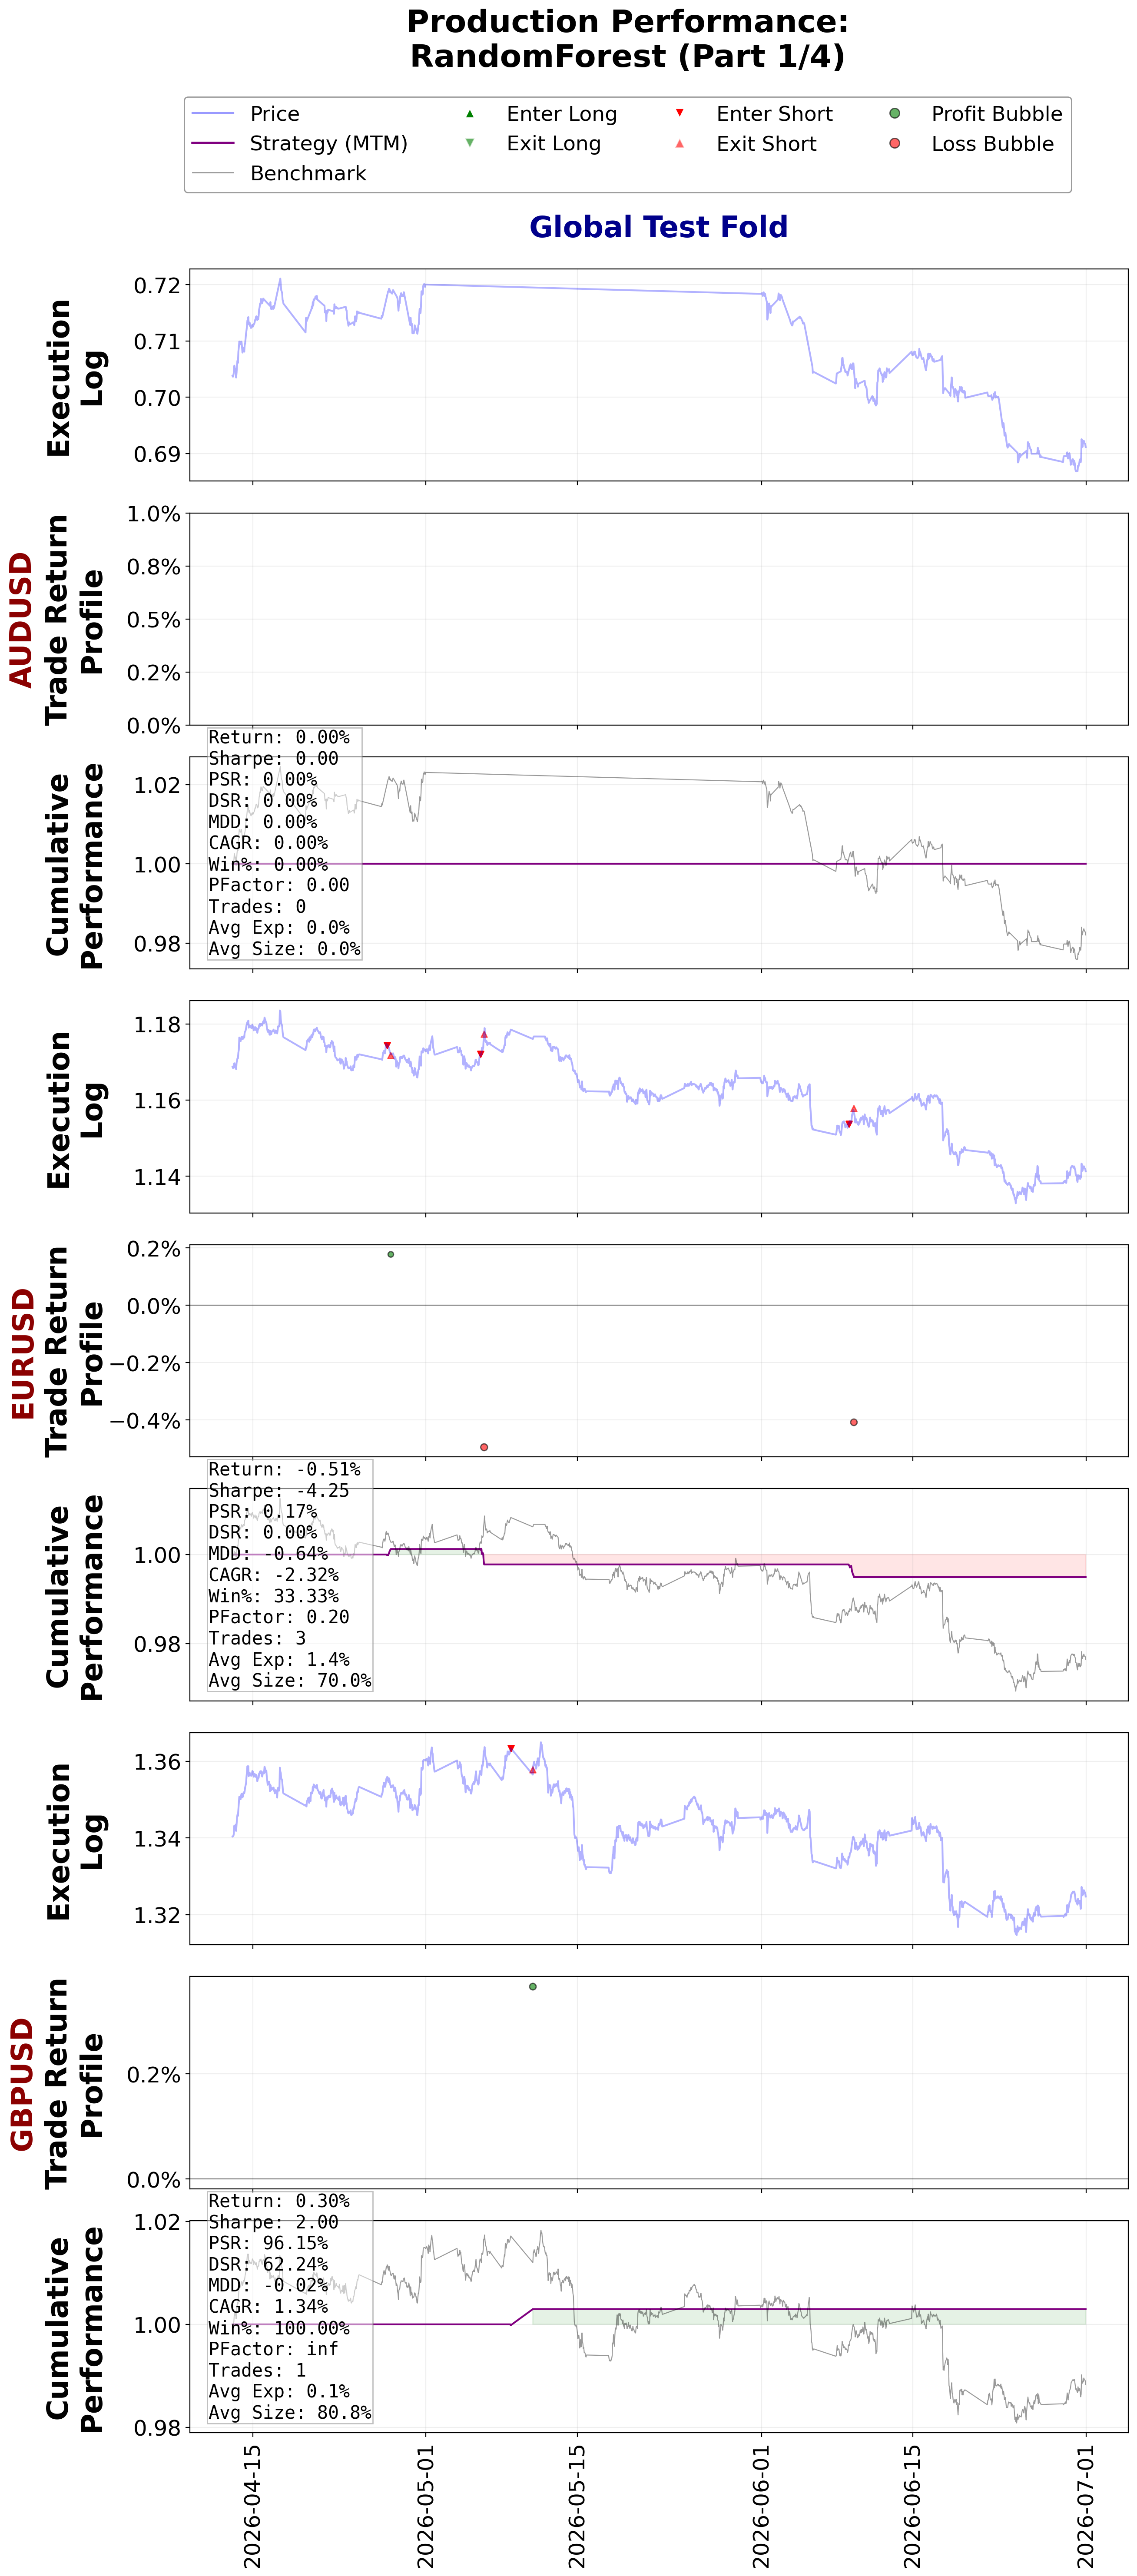
\includegraphics[width=\textwidth]{../data/figures/backtests/production_results_RandomForest_part1.png}
        \caption{Backtest Result of RandomForest During Production}
        \label{fig:production_result_RandomForest_1}
    \end{minipage}
    \hfill
    \begin{minipage}[t]{0.49\textwidth}
        \centering
        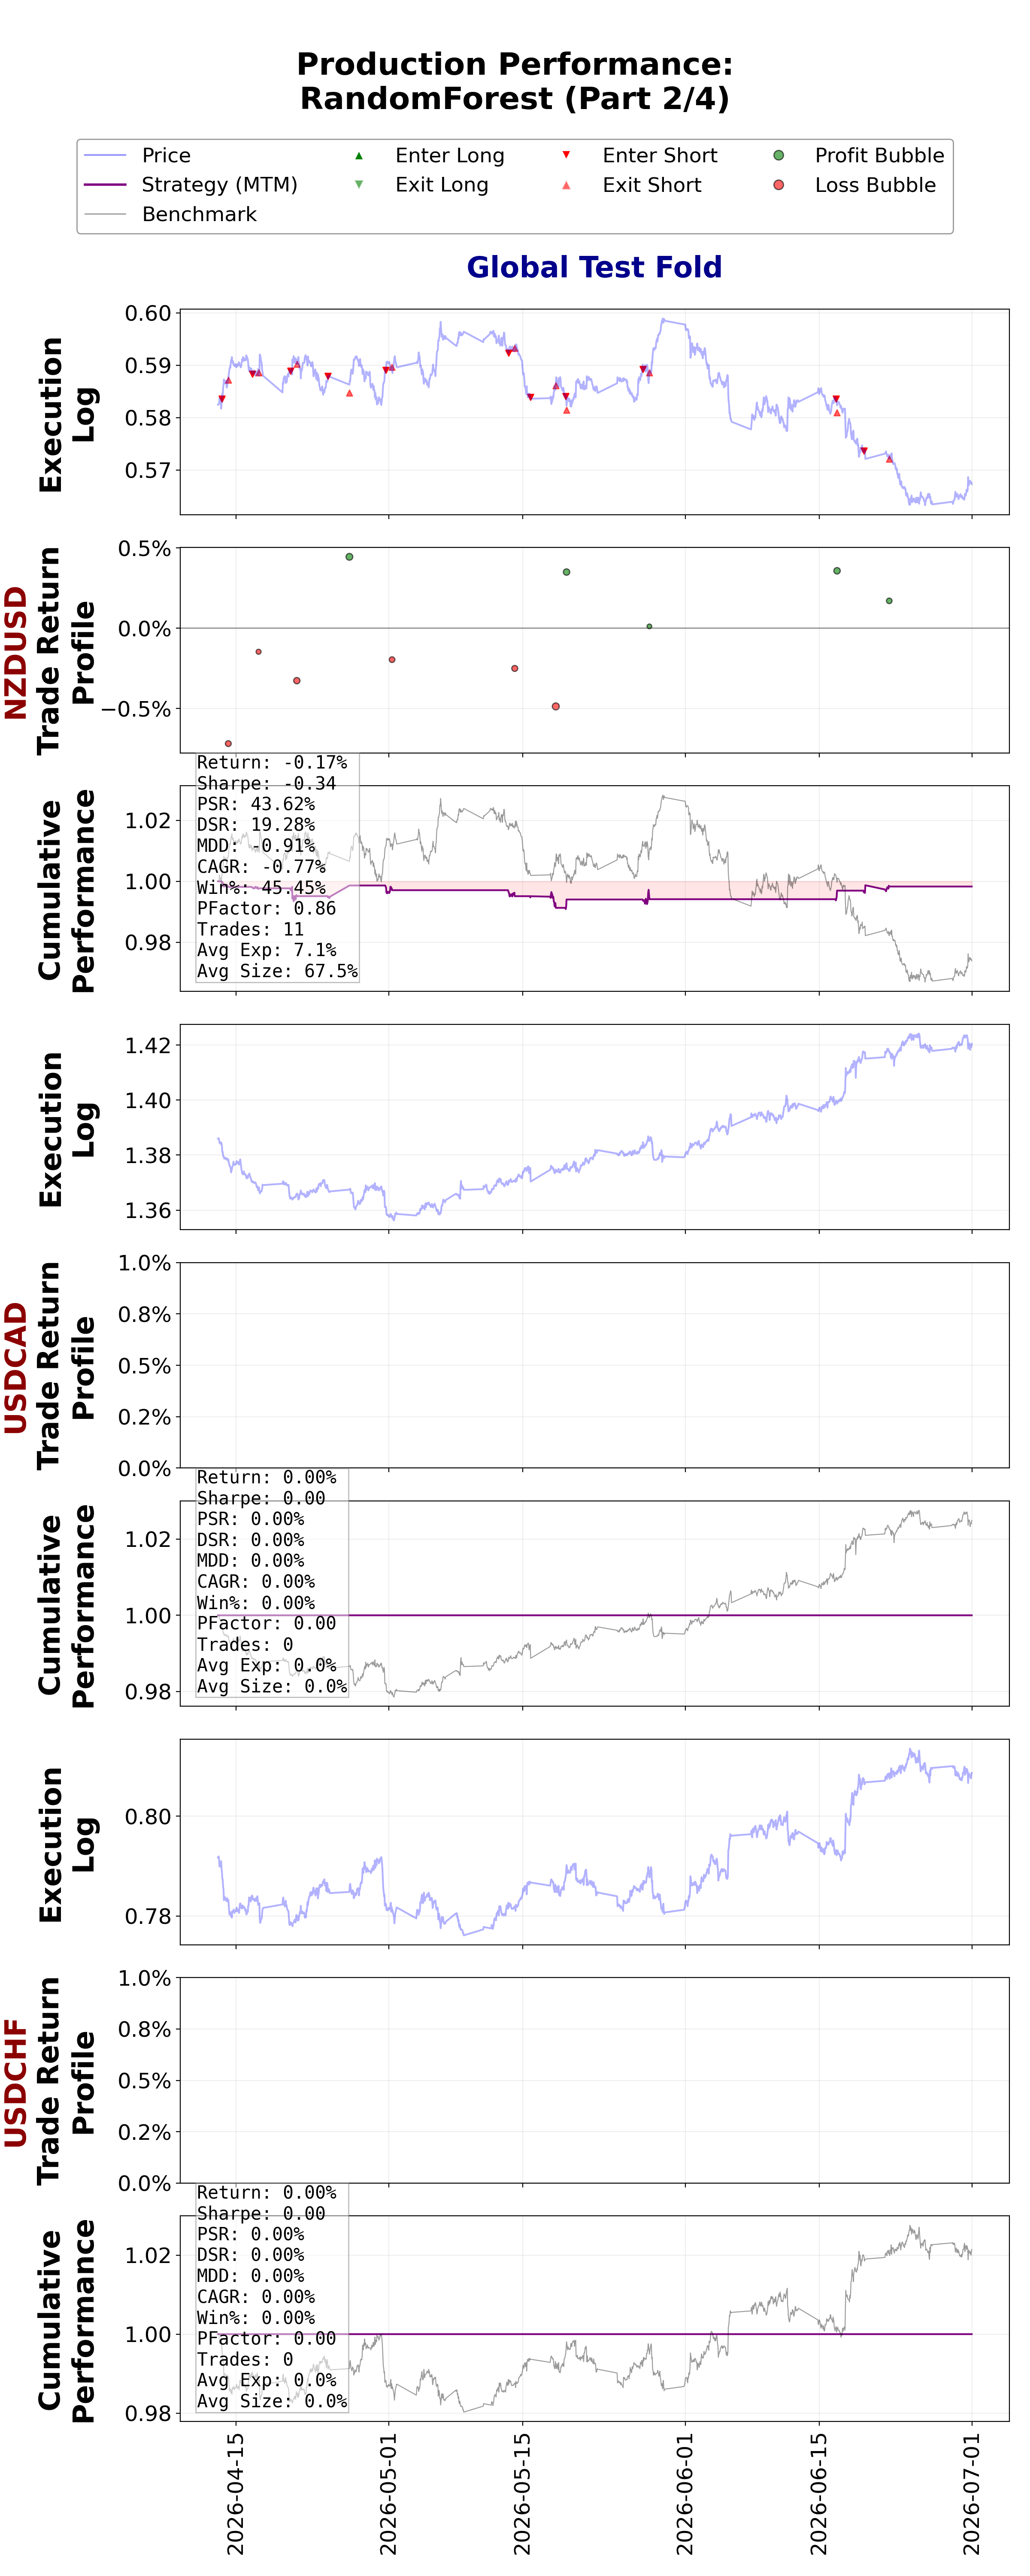
\includegraphics[width=\textwidth]{../data/figures/backtests/production_results_RandomForest_part2.png}
        \caption{Backtest Result of RandomForest During Production (Continued)}
        \label{fig:production_result_RandomForest_2}
    \end{minipage}
\end{figure}

\begin{figure}[H]
    \centering
    \begin{minipage}[t]{0.49\textwidth}
        \centering
        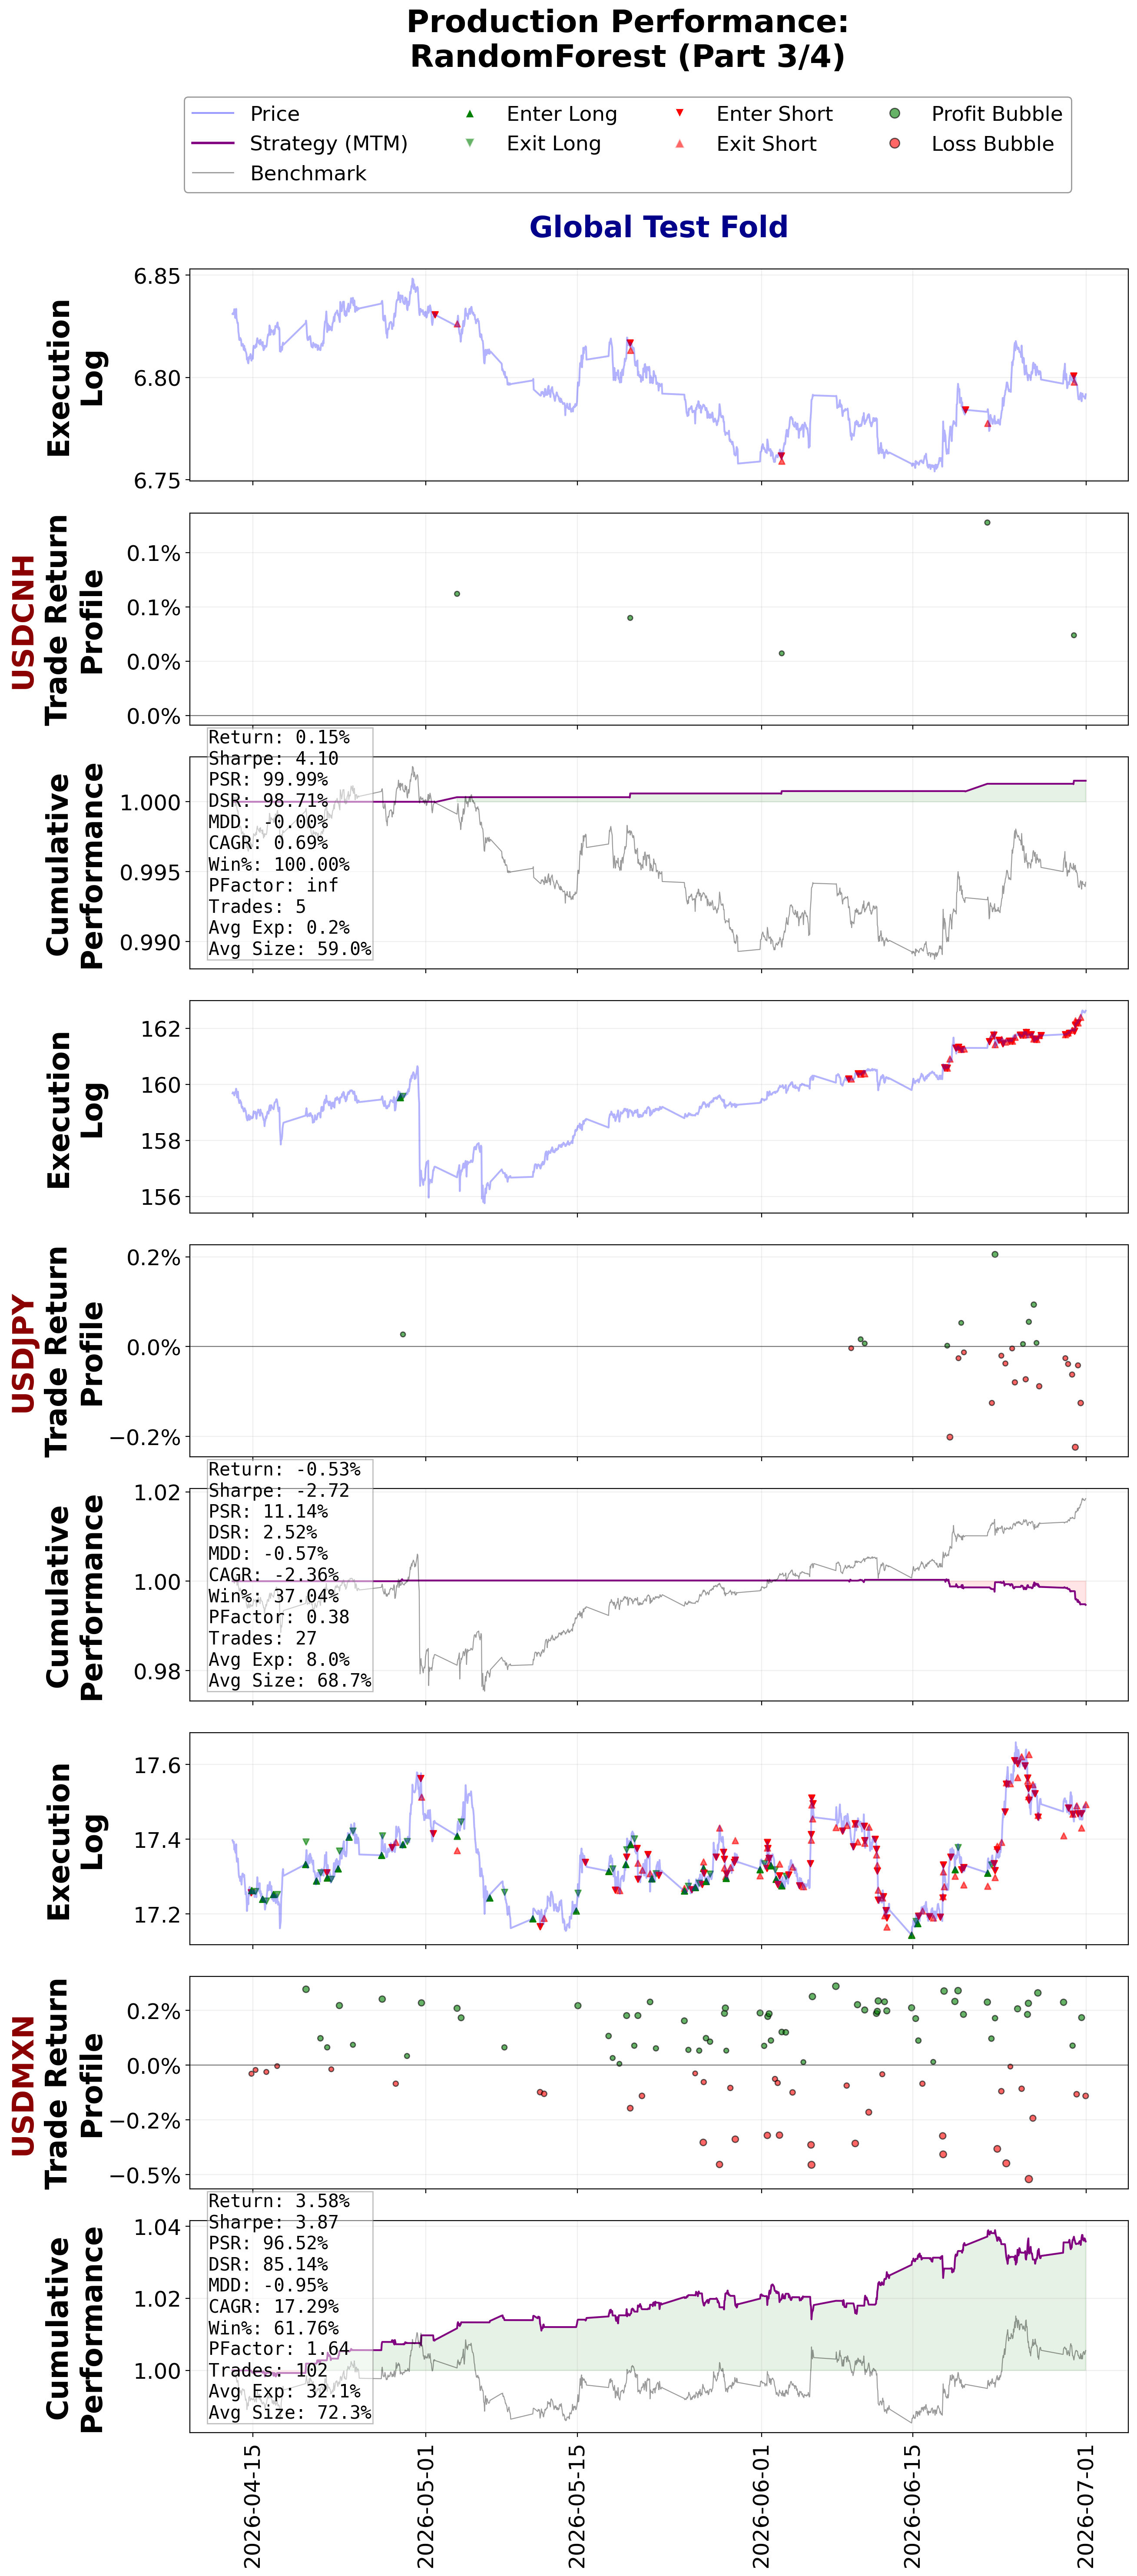
\includegraphics[width=\textwidth]{../data/figures/backtests/production_results_RandomForest_part3.png}
        \caption{Backtest Result of RandomForest During Production (Continued)}
        \label{fig:production_result_RandomForest_3}
    \end{minipage}
    \hfill
    \begin{minipage}[t]{0.49\textwidth}
        \centering
        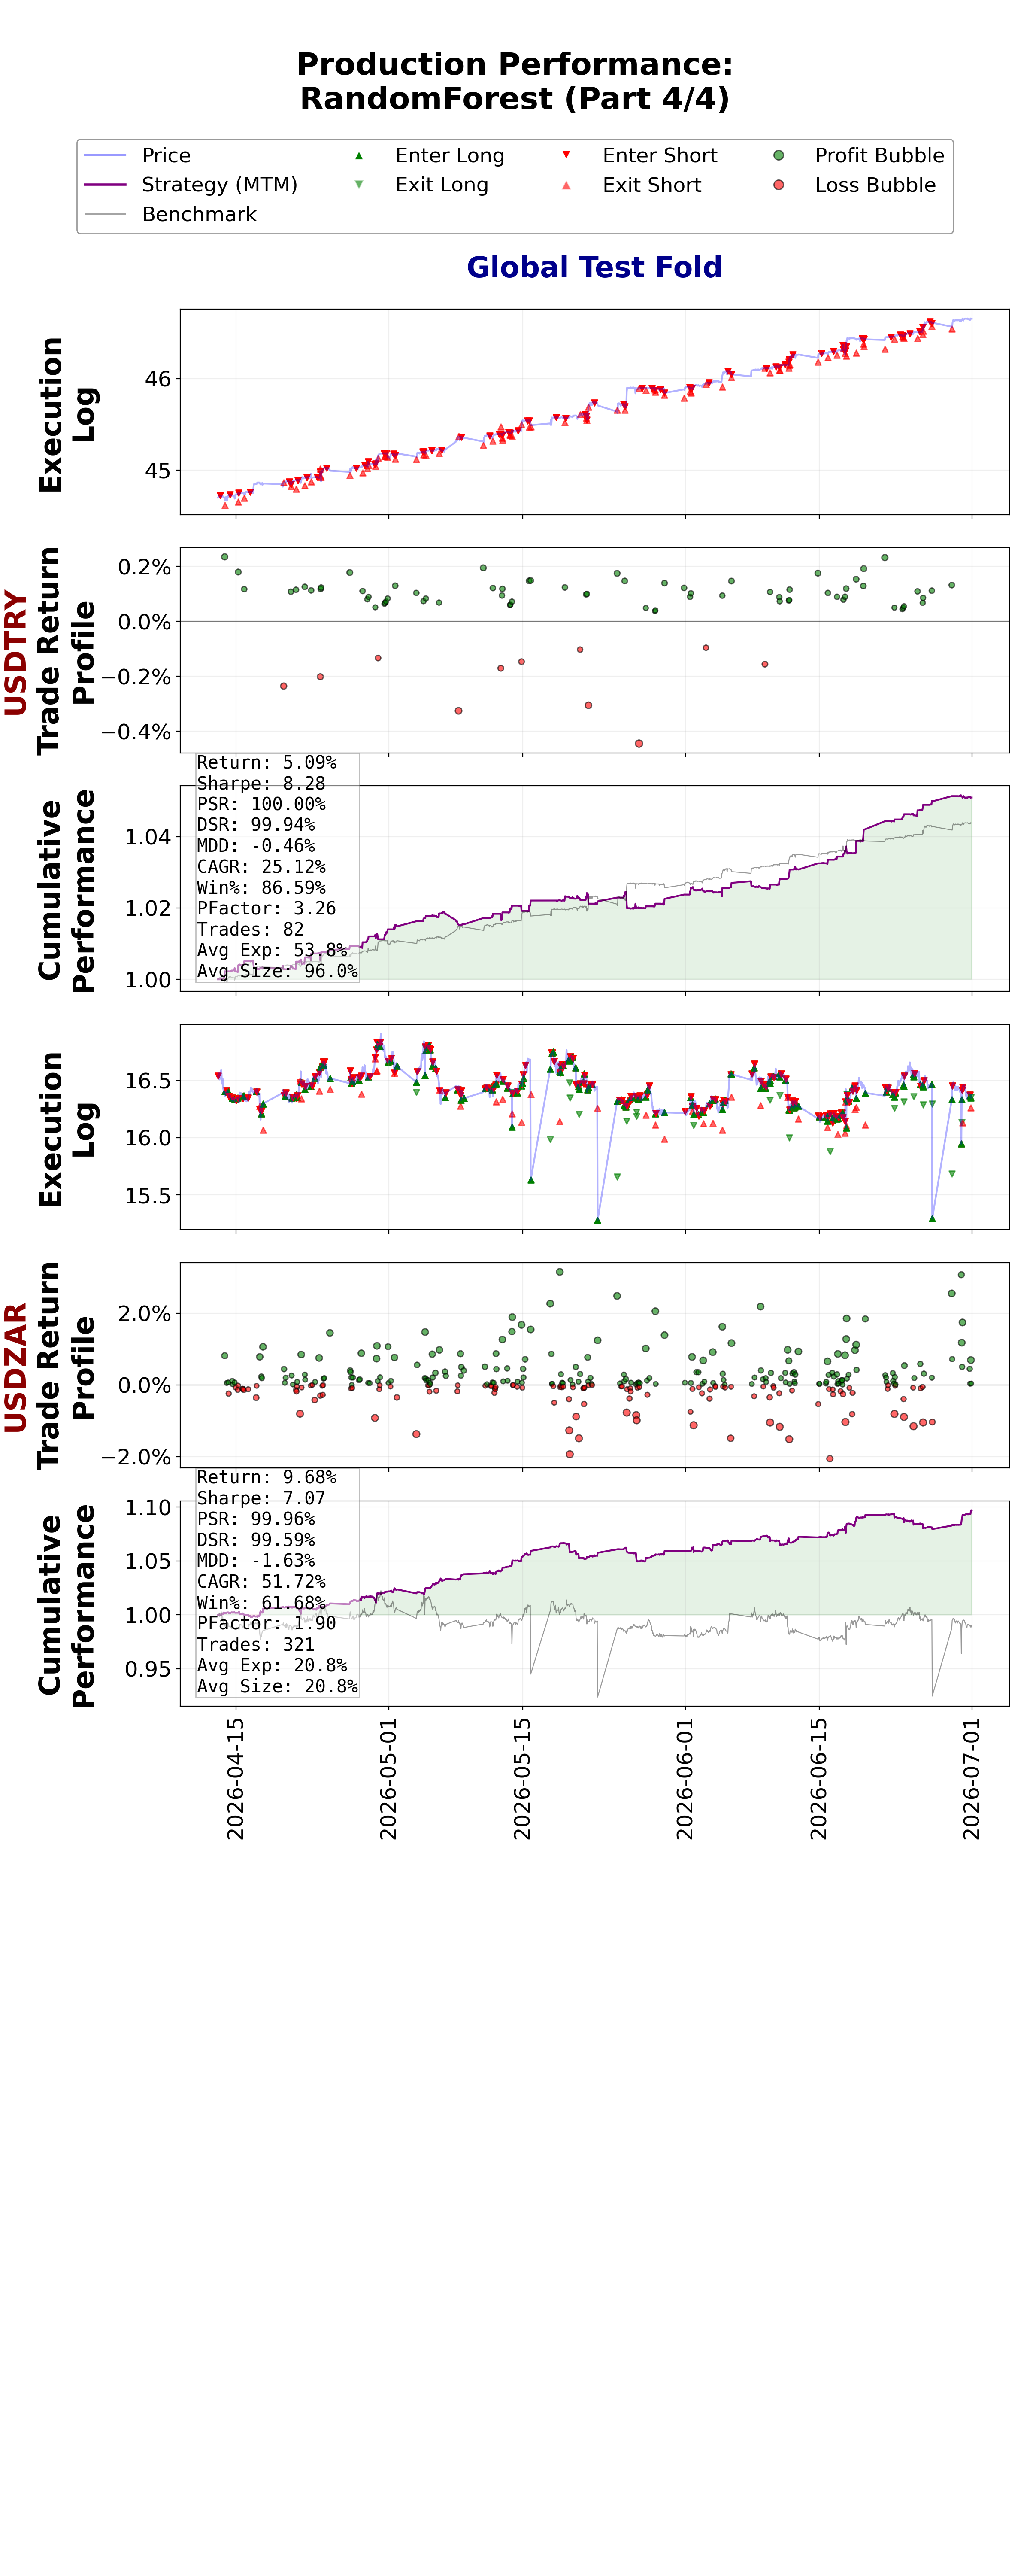
\includegraphics[width=\textwidth]{../data/figures/backtests/production_results_RandomForest_part4.png}
        \caption{Backtest Result of RandomForest During Production (Continued)}
        \label{fig:production_result_RandomForest_4}
    \end{minipage}
\end{figure}

%%%%%%%%%%%%%%%%%%%%%%%%%%%%%%%%%%%%%%%%%%%%%%%%%%%%%%%%%%%%%%%%%%%%%%%%%%%%%%%%%%%%%%%%%%%%%%%%%%%%%%%%%%%%%%%%%%%%%%%%%%%
%%%%%%%%%%%%%%%%%%%%%%%%%%%%%%%%%%%%%%%%%%%%%%%%%%%%%%%%%%%%%%%%%%%%%%%%%%%%%%%%%%%%%%%%%%%%%%%%%%%%%%%%%%%%%%%%%%%%%%%%%%%
Lorem ipsum dolor sit amet, consectetur adipiscing elit. Sed do eiusmod tempor incididunt ut labore et dolore magna aliqua. 
Ut enim ad minim veniam, quis nostrud exercitation ullamco laboris nisi ut aliquip ex ea commodo consequat. 
Duis aute irure dolor in reprehenderit in voluptate velit esse cillum dolore eu fugiat nulla pariatur. 
Excepteur sint occaecat cupidatat non proident, sunt in culpa qui officia deserunt mollit anim id est laborum
Lorem ipsum dolor sit amet, consectetur adipiscing elit. Sed do eiusmod tempor incididunt ut labore et dolore magna aliqua. 
Ut enim ad minim veniam, quis nostrud exercitation ullamco laboris nisi ut aliquip ex ea commodo consequat. 
Duis aute irure dolor in reprehenderit in voluptate velit esse cillum dolore eu fugiat nulla pariatur. 
Excepteur sint occaecat cupidatat non proident, sunt in culpa qui officia deserunt mollit anim id est laborum
Lorem ipsum dolor sit amet, consectetur adipiscing elit. Sed do eiusmod tempor incididunt ut labore et dolore magna aliqua. 
Ut enim ad minim veniam, quis nostrud exercitation ullamco laboris nisi ut aliquip ex ea commodo consequat. 
Duis aute irure dolor in reprehenderit in voluptate velit esse cillum dolore eu fugiat nulla pariatur. 
Excepteur sint occaecat cupidatat non proident, sunt in culpa qui officia deserunt mollit anim id est laborum
%%%%%%%%%%%%%%%%%%%%%%%%%%%%%%%%%%%%%%%%%%%%%%%%%%%%%%%%%%%%%%%%%%%%%%%%%%%%%%%%%%%%%%%%%%%%%%%%%%%%%%%%%%%%%%%%%%%%%%%%%%%
%%%%%%%%%%%%%%%%%%%%%%%%%%%%%%%%%%%%%%%%%%%%%%%%%%%%%%%%%%%%%%%%%%%%%%%%%%%%%%%%%%%%%%%%%%%%%%%%%%%%%%%%%%%%%%%%%%%%%%%%%%%

\begin{table}[H]
\centering
\caption{{Granular Performance Analysis RandomForest (Production Phase)}}
\label{tab:perf_RandomForest_production}
\resizebox{\textwidth}{!}{\begin{tabular}{rrrrrrrrrrrrrr}
\toprule
Pair & Fold & \rotatebox{90}{Total Return (\%)} & \rotatebox{90}{Sharpe Ratio} & \rotatebox{90}{Probabilistic Sharpe (\%)} & \rotatebox{90}{Max Drawdown (\%)} & \rotatebox{90}{CAGR (\%)} & \rotatebox{90}{Win Rate (\%)} & \rotatebox{90}{Profit Factor} & \rotatebox{90}{Number of Trades} & \rotatebox{90}{Avg Capital Exposure (\%)} & \rotatebox{90}{Avg Trade Size (\%)} & \rotatebox{90}{Deflated Sharpe (\%)} & \rotatebox{90}{M2 Brier} \\
\midrule
AUDUSD & Fold 1 & 0.0000\% & 0.0000 & 0.0000\% & 0.0000\% & 0.0000\% & 0.0000\% & 0.0000 & 0.0000 & 0.0000\% & 0.0000\% & 0.0000\% & 0.24 \\
EURUSD & Fold 1 & -0.41\% & -3.66 & 1.41\% & -0.47\% & -1.86\% & 42.86\% & 0.17 & 7.00 & 1.34\% & 49.01\% & 0.10\% & 0.24 \\
GBPUSD & Fold 1 & 0.75\% & 2.60 & 94.18\% & -0.39\% & 3.42\% & 100.00\% & inf & 3.00 & 4.30\% & 59.38\% & 74.43\% & 0.24 \\
NZDUSD & Fold 1 & -0.17\% & -0.34 & 43.62\% & -0.91\% & -0.77\% & 45.45\% & 0.86 & 11.00 & 7.06\% & 67.45\% & 19.28\% & 0.24 \\
USDCAD & Fold 1 & 0.0000\% & 0.0000 & 0.0000\% & 0.0000\% & 0.0000\% & 0.0000\% & 0.0000 & 0.0000 & 0.0000\% & 0.0000\% & 0.0000\% & 0.24 \\
USDCHF & Fold 1 & 0.0000\% & 0.0000 & 0.0000\% & 0.0000\% & 0.0000\% & 0.0000\% & 0.0000 & 0.0000 & 0.0000\% & 0.0000\% & 0.0000\% & 0.24 \\
USDCNH & Fold 1 & 0.95\% & 7.10 & 99.97\% & -0.16\% & 4.41\% & 80.95\% & 2.66 & 63.00 & 10.35\% & 47.70\% & 99.69\% & 0.24 \\
USDJPY & Fold 1 & -0.84\% & -2.23 & 14.75\% & -1.29\% & -3.73\% & 42.37\% & 0.68 & 59.00 & 21.87\% & 68.69\% & 3.93\% & 0.24 \\
USDMXN & Fold 1 & 9.18\% & 14.34 & 100.00\% & -0.59\% & 48.93\% & 71.21\% & 2.27 & 514.00 & 31.71\% & 32.00\% & 100.00\% & 0.24 \\
USDTRY & Fold 1 & 5.09\% & 8.28 & 100.00\% & -0.46\% & 25.12\% & 86.59\% & 3.26 & 82.00 & 53.79\% & 96.04\% & 99.94\% & 0.24 \\
USDZAR & Fold 1 & 9.68\% & 7.07 & 99.96\% & -1.63\% & 51.72\% & 61.68\% & 1.90 & 321.00 & 20.83\% & 20.83\% & 99.59\% & 0.24 \\
\midrule
\midrule
Fold 1 Avg &  & \shortstack{2.20\% \\ $\pm$ 3.91\%} & \shortstack{3.01 \\ $\pm$ 5.48} & \shortstack{50.35\% \\ $\pm$ 48.05\%} & \shortstack{-0.54\% \\ $\pm$ 0.54\%} & \shortstack{11.57\% \\ $\pm$ 20.68\%} & \shortstack{48.28\% \\ $\pm$ 36.03\%} & \shortstack{inf \\ $\pm$ nan} & \shortstack{96.36 \\ $\pm$ 167.17} & \shortstack{13.75\% \\ $\pm$ 17.05\%} & \shortstack{40.10\% \\ $\pm$ 32.35\%} & \shortstack{45.18\% \\ $\pm$ 48.29\%} & \shortstack{0.24 \\ $\pm$ 0.0000} \\
Total Avg &  & \shortstack{2.20\% \\ $\pm$ 3.91\%} & \shortstack{3.01 \\ $\pm$ 5.48} & \shortstack{50.35\% \\ $\pm$ 48.05\%} & \shortstack{-0.54\% \\ $\pm$ 0.54\%} & \shortstack{11.57\% \\ $\pm$ 20.68\%} & \shortstack{48.28\% \\ $\pm$ 36.03\%} & \shortstack{inf \\ $\pm$ nan} & \shortstack{96.36 \\ $\pm$ 167.17} & \shortstack{13.75\% \\ $\pm$ 17.05\%} & \shortstack{40.10\% \\ $\pm$ 32.35\%} & \shortstack{45.18\% \\ $\pm$ 48.29\%} & \shortstack{0.24 \\ $\pm$ 0.0000} \\
\bottomrule
\end{tabular}}
\end{table}


\begin{table}[H]
\centering
\caption{{Cross-Strategy Performance Comparison: RandomForest (Production Phase) - Annualized Sharpe Ratio}}
\label{tab:strategy_comparison_RandomForest_production}
\resizebox{\textwidth}{!}{\begin{tabular}{llllllll}
\toprule
Fold & Pair & Buy and Hold & SMA Crossover & M1 Only & M1 + M2 (Fixed) & M1 + M2 (Global) & M1 + M2 (Conformal) \\
\midrule
Fold 1 & AUDUSD & -1.83 & 3.75 & -2.76 & -2.86 & 0.00 & 0.00 \\
 & EURUSD & -2.02 & -1.52 & -5.86 & -5.10 & -3.81 & -4.25 \\
 & GBPUSD & -0.82 & -3.50 & -2.93 & -2.96 & 0.00 & 2.00 \\
 & NZDUSD & -1.32 & -1.12 & -4.37 & -3.42 & 0.00 & 0.00 \\
 & USDCAD & 2.47 & 2.03 & 0.17 & -1.46 & 2.62 & 2.87 \\
 & USDCHF & 1.47 & -2.60 & -10.40 & -9.89 & 0.00 & 0.00 \\
 & USDCNH & -1.05 & -1.02 & -2.39 & -2.07 & 5.12 & 4.10 \\
 & USDJPY & 1.27 & -0.01 & 5.97 & 4.70 & -1.61 & -2.72 \\
 & USDMXN & 0.36 & -3.48 & 13.02 & 13.02 & 1.56 & 3.87 \\
 & USDTRY & 7.83 & 7.31 & 14.79 & 14.36 & 7.08 & 5.58 \\
 & USDZAR & 0.08 & -0.61 & 11.42 & 11.46 & 9.89 & 5.19 \\
\midrule
 & \textbf{AVERAGE} & \textbf{0.59 ($\pm$ 2.80)} & \textbf{-0.07 ($\pm$ 3.28)} & \textbf{1.51 ($\pm$ 8.44)} & \textbf{1.43 ($\pm$ 8.16)} & \textbf{1.90 ($\pm$ 4.01)} & \textbf{1.51 ($\pm$ 3.20)} \\
\midrule
\bottomrule
\end{tabular}}
\end{table}


%%%%%%%%%%%%%%%%%%%%%%%%%%%%%%%%%%%%%%%%%%%%%%%%%%%%%%%%%%%%%%%%%%%%%%%%%%%%%%%%%%%%%%%%%%%%%%%%%%%%%%%%%%%%%%%%%%%%%%%%%%%
%%%%%%%%%%%%%%%%%%%%%%%%%%%%%%%%%%%%%%%%%%%%%%%%%%%%%%%%%%%%%%%%%%%%%%%%%%%%%%%%%%%%%%%%%%%%%%%%%%%%%%%%%%%%%%%%%%%%%%%%%%%
Lorem ipsum dolor sit amet, consectetur adipiscing elit. Sed do eiusmod tempor incididunt ut labore et dolore magna aliqua. 
Ut enim ad minim veniam, quis nostrud exercitation ullamco laboris nisi ut aliquip ex ea commodo consequat. 
Duis aute irure dolor in reprehenderit in voluptate velit esse cillum dolore eu fugiat nulla pariatur. 
Excepteur sint occaecat cupidatat non proident, sunt in culpa qui officia deserunt mollit anim id est laborum
Lorem ipsum dolor sit amet, consectetur adipiscing elit. Sed do eiusmod tempor incididunt ut labore et dolore magna aliqua. 
Ut enim ad minim veniam, quis nostrud exercitation ullamco laboris nisi ut aliquip ex ea commodo consequat. 
Duis aute irure dolor in reprehenderit in voluptate velit esse cillum dolore eu fugiat nulla pariatur. 
Excepteur sint occaecat cupidatat non proident, sunt in culpa qui officia deserunt mollit anim id est laborum
Lorem ipsum dolor sit amet, consectetur adipiscing elit. Sed do eiusmod tempor incididunt ut labore et dolore magna aliqua. 
Ut enim ad minim veniam, quis nostrud exercitation ullamco laboris nisi ut aliquip ex ea commodo consequat. 
Duis aute irure dolor in reprehenderit in voluptate velit esse cillum dolore eu fugiat nulla pariatur. 
Excepteur sint occaecat cupidatat non proident, sunt in culpa qui officia deserunt mollit anim id est laborum
%%%%%%%%%%%%%%%%%%%%%%%%%%%%%%%%%%%%%%%%%%%%%%%%%%%%%%%%%%%%%%%%%%%%%%%%%%%%%%%%%%%%%%%%%%%%%%%%%%%%%%%%%%%%%%%%%%%%%%%%%%%
%%%%%%%%%%%%%%%%%%%%%%%%%%%%%%%%%%%%%%%%%%%%%%%%%%%%%%%%%%%%%%%%%%%%%%%%%%%%%%%%%%%%%%%%%%%%%%%%%%%%%%%%%%%%%%%%%%%%%%%%%%%

\begin{table}[H] \centering
\caption{RRF Granular Rankings (Production Phase)}
\label{tab:rrf_matrix_production}
\small \begin{tabular}{l l c}
\toprule
Currency Pair & Fold & \rotatebox{90}{RandomForest} \\
\midrule
AUDUSD & Fold 1 & 6 (0.120) \\
EURUSD & Fold 1 & 10 (0.117) \\
GBPUSD & Fold 1 & 4 (0.125) \\
NZDUSD & Fold 1 & 9 (0.119) \\
USDCAD & Fold 1 & 6 (0.120) \\
USDCHF & Fold 1 & 6 (0.120) \\
USDCNH & Fold 1 & 3 (0.126) \\
USDJPY & Fold 1 & 11 (0.116) \\
USDMXN & Fold 1 & 2 (0.127) \\
USDTRY & Fold 1 & 1 (0.128) \\
USDZAR & Fold 1 & 5 (0.125) \\
\bottomrule
\end{tabular}
\end{table}

\begin{table}[H]
\caption{RRF Performance Summary: Best and Worst Performing Pairs (Production Phase)}
\label{tab:rrf_summary_production}
\begin{tabular}{l l p{5cm} p{5cm}}
\toprule
Model & Fold & Best Performers (RRF) & Worst Performers (RRF) \\
\midrule
RandomForest & Fold 1 & USDCNH, USDTRY & EURUSD, USDJPY \\
\bottomrule
\end{tabular}
\end{table}


%%%%%%%%%%%%%%%%%%%%%%%%%%%%%%%%%%%%%%%%%%%%%%%%%%%%%%%%%%%%%%%%%%%%%%%%%%%%%%%%%%%%%%%%%%%%%%%%%%%%%%%%%%%%%%%%%%%%%%%%%%%
%%%%%%%%%%%%%%%%%%%%%%%%%%%%%%%%%%%%%%%%%%%%%%%%%%%%%%%%%%%%%%%%%%%%%%%%%%%%%%%%%%%%%%%%%%%%%%%%%%%%%%%%%%%%%%%%%%%%%%%%%%%
Lorem ipsum dolor sit amet, consectetur adipiscing elit. Sed do eiusmod tempor incididunt ut labore et dolore magna aliqua. 
Ut enim ad minim veniam, quis nostrud exercitation ullamco laboris nisi ut aliquip ex ea commodo consequat. 
Duis aute irure dolor in reprehenderit in voluptate velit esse cillum dolore eu fugiat nulla pariatur. 
Excepteur sint occaecat cupidatat non proident, sunt in culpa qui officia deserunt mollit anim id est laborum
Lorem ipsum dolor sit amet, consectetur adipiscing elit. Sed do eiusmod tempor incididunt ut labore et dolore magna aliqua. 
Ut enim ad minim veniam, quis nostrud exercitation ullamco laboris nisi ut aliquip ex ea commodo consequat. 
Duis aute irure dolor in reprehenderit in voluptate velit esse cillum dolore eu fugiat nulla pariatur. 
Excepteur sint occaecat cupidatat non proident, sunt in culpa qui officia deserunt mollit anim id est laborum
Lorem ipsum dolor sit amet, consectetur adipiscing elit. Sed do eiusmod tempor incididunt ut labore et dolore magna aliqua. 
Ut enim ad minim veniam, quis nostrud exercitation ullamco laboris nisi ut aliquip ex ea commodo consequat. 
Duis aute irure dolor in reprehenderit in voluptate velit esse cillum dolore eu fugiat nulla pariatur. 
Excepteur sint occaecat cupidatat non proident, sunt in culpa qui officia deserunt mollit anim id est laborum
%%%%%%%%%%%%%%%%%%%%%%%%%%%%%%%%%%%%%%%%%%%%%%%%%%%%%%%%%%%%%%%%%%%%%%%%%%%%%%%%%%%%%%%%%%%%%%%%%%%%%%%%%%%%%%%%%%%%%%%%%%%
%%%%%%%%%%%%%%%%%%%%%%%%%%%%%%%%%%%%%%%%%%%%%%%%%%%%%%%%%%%%%%%%%%%%%%%%%%%%%%%%%%%%%%%%%%%%%%%%%%%%%%%%%%%%%%%%%%%%%%%%%%%


\subsubsection{Tournament vs. Production: Robustness \& Performance Consistency}
- comparison tables of ie financial statistics like sharpe etc (Metric / Tournament (mean) / Production / Change)
- talk about best/worst performing pairs between tournament and production model but put the table in appendix

%%%%%%%%%%%%%%%%%%%%%%%%%%%%%%%%%%%%%%%%%%%%%%%%%%%%%%%%%%%%%%%%%%%%%%%%%%%%%%%%%%%%%%%%%%%%%%%%%%%%%%%%%%%%%%%%%%%%%%%%%%%
%%%%%%%%%%%%%%%%%%%%%%%%%%%%%%%%%%%%%%%%%%%%%%%%%%%%%%%%%%%%%%%%%%%%%%%%%%%%%%%%%%%%%%%%%%%%%%%%%%%%%%%%%%%%%%%%%%%%%%%%%%%
Lorem ipsum dolor sit amet, consectetur adipiscing elit. Sed do eiusmod tempor incididunt ut labore et dolore magna aliqua. 
Ut enim ad minim veniam, quis nostrud exercitation ullamco laboris nisi ut aliquip ex ea commodo consequat. 
Duis aute irure dolor in reprehenderit in voluptate velit esse cillum dolore eu fugiat nulla pariatur. 
Excepteur sint occaecat cupidatat non proident, sunt in culpa qui officia deserunt mollit anim id est laborum
Lorem ipsum dolor sit amet, consectetur adipiscing elit. Sed do eiusmod tempor incididunt ut labore et dolore magna aliqua. 
Ut enim ad minim veniam, quis nostrud exercitation ullamco laboris nisi ut aliquip ex ea commodo consequat. 
Duis aute irure dolor in reprehenderit in voluptate velit esse cillum dolore eu fugiat nulla pariatur. 
Excepteur sint occaecat cupidatat non proident, sunt in culpa qui officia deserunt mollit anim id est laborum
Lorem ipsum dolor sit amet, consectetur adipiscing elit. Sed do eiusmod tempor incididunt ut labore et dolore magna aliqua. 
Ut enim ad minim veniam, quis nostrud exercitation ullamco laboris nisi ut aliquip ex ea commodo consequat. 
Duis aute irure dolor in reprehenderit in voluptate velit esse cillum dolore eu fugiat nulla pariatur. 
Excepteur sint occaecat cupidatat non proident, sunt in culpa qui officia deserunt mollit anim id est laborum
%%%%%%%%%%%%%%%%%%%%%%%%%%%%%%%%%%%%%%%%%%%%%%%%%%%%%%%%%%%%%%%%%%%%%%%%%%%%%%%%%%%%%%%%%%%%%%%%%%%%%%%%%%%%%%%%%%%%%%%%%%%
%%%%%%%%%%%%%%%%%%%%%%%%%%%%%%%%%%%%%%%%%%%%%%%%%%%%%%%%%%%%%%%%%%%%%%%%%%%%%%%%%%%%%%%%%%%%%%%%%%%%%%%%%%%%%%%%%%%%%%%%%%%

%%%%%%%%%%%%%%
% DISCUSSION %
%%%%%%%%%%%%%%
\section{Discussion}

%%%%%%%%%%%%%%
% CONCLUSION %
%%%%%%%%%%%%%%
\section{Conclusion and Future Work}
\subsection{Summary}
The Efficacy of Meta-Labeling in Forex


\subsection{Future Extensions}

\subsubsection{Refactoring of the Codebase}

The current implementation, while functionally adequate for the scope of this thesis, is organized as a set of tightly connected, procedural scripts rather than a 
modular software architecture. Data acquisition, model training, conformal calibration, and order execution are frequently interleaved within the same function 
bodies and share mutable state across long-running loops, which makes unit testing individual components in isolation difficult. 
A more maintainable direction, sketched in \ref{app:code refactored}, would separate the system into a domain layer of data classes 
(MarketData and Signal), and three interfaces for data acquisition, strategy generation, and execution, which will be coordinated through a thin 
TradingSystemFacade. Under this design, concrete implementations (e.g. an IBKR\_MarketDataFeed or a BacktestSimEngine) become interchangeable behind their 
respective interfaces (IDataProvider and IExecutionEngine), allowing the same strategy logic to run unmodified against a live broker or a historical simulation. 
Furthermore, the conformal veto could similarly be expressed as a decorator (ConformalVetoDecorator) wrapping an inner IStrategy, rather than being hard-coded into 
the signal generation path. It should be stressed that this diagram is illustrative rather than a finished architecture and is intended merely to gesture toward the 
SOLID design principles, adherence to which was not a concern of this thesis. Adopting such a structure would not, by itself, resolve the statistical subtleties 
uncovered in this study but rather it would reduce the engineering risk of introducing or hiding such issues in the first place, while meaningfully easing the 
future extensions proposed below.


\subsubsection{Data Quality}

While this study maintains high standards for data integrity through rigorous Sanity Checks (\ref{sec:sanity_checks}), a primary area for future extension is the further hardening of the 
underlying data source. Our current pipeline orchestrates the merging of Polygon.io (via OpenBB) for primary transaction data and Dukascopy for binary-decoded bid/ask spreads
and thus relies on a naive UTC timestamp synchronization (see \ref{sec:data_acquisition}). While every precaution was taken to ensure temporal alignment, the lack of a unified,
high-precision institutional primary key (such as millisecond-accurate FIX sequence numbers) leaves a non-zero margin for micro-gaps or off-by-one errors during the left-join process.
Consequently, future research should explore the utilization of a unified institutional liquidity provider (e.g., LMAX Exchange, Bloomberg, or Interactive Brokers' IDB feed). 
Sourcing transaction prices and spreads from a single engine would eliminate the need for heuristic temporal merging and provide a more robust ground truth for the M2 meta-model. 
Furthermore, extending the dataset to include tick-level order flow (Level 2 data) would allow the meta-model to move beyond simple OHLCV features and audit the efficacy of the conformal 
veto logic within the context of market depth and order book imbalances.


\subsubsection{More Insightful Feature Engineering}

A primary limitation of the feature engineering framework discussed in \ref{sec:features_labels} is its exclusive reliance on endogenous variables. 
While our current suite of, among others, momentum, volatility, and microstructural indicators provides a high-fidelity mapping of the instrument's own price-action
dynamics, it operates within a macroeconomic vacuum. In the highly integrated global Forex market, currency valuations are fundamentally driven by inter-market relative value and 
sovereign yield differentials. To move beyond the limitations of univariate price analysis, future extensions should incorporate exogenous features that capture the broader economic landscape. 
Specifically, the integration of interest rate differentials (using 2-year and 10-year Treasury yield spreads), global equity market volatility (VIX), and commodity price indices 
(e.g., WTI Crude for the CAD, or Gold for the AUD) could provide the meta-model with critical market regime context. These data streams could be sourced through high-frequency 
macroeconomic APIs such as the Federal Reserve Economic Data (FRED) or Refinitiv Eikon. By augmenting the M1 signal generator with these external pressures, the meta-model (M2)
could develop a more nuanced understanding of when a technical signal is aligned with or fighting against fundamental capital flows, thereby further refining the efficacy of the 
conformal veto logic.


%%%%%%%%%%%%%%%%
% BIBLIOGRAPHY %
%%%%%%%%%%%%%%%%
\section{References}
\printbibliography[heading=none]

%%%%%%%%%%%%
% APPENDIX %
%%%%%%%%%%%%
\section{Appendix}
\appendix


\section{Evaluation Metrics}\label{app:metrics}

The primary measure of risk-adjusted return is the Sharpe Ratio, which we calculate using arithmetic returns \( r_t = \frac{(E_t - E_{t-1})}{E_{t-1}} \). 
To ensure comparability across different time horizons, the ratio is annualized as follows:

\begin{equation}
    \text{SR} = \frac{\overline{r}}{\sigma_{r}} \times \sqrt{N}
    \label{eq:sharpe_ratio}
\end{equation}

where $\overline{r}$ is the mean return, $\sigma_{r}$ is the standard deviation of returns, and N is the annualization factor (i.e., N=252 $\times$ 24 for hourly data).
Unlike simple average returns, the compund annual growth rate (CAGR) represents the annualized geometric mean return that would provide the same final equity from the initial capital over time, 
accounting for the compounding effect:

\begin{equation}
    \text{CAGR} = \left( \frac{E_T}{E_0} \right)^{\frac{1}{y}} - 1
    \label{eq:cagr}
\end{equation}

where $E_T$ is the final equity, $E_0$ is the initial capital, and y is the total elapsed time in years.
The maximum drawdown (MDD) measures the largest peak-to-trough decline in the account's history, serving as the primary indicator of absolute risk and investor pain:

\begin{equation}
    \text{MDD} = \max_{0 \leq t \leq T} \left( \frac{ \max_{0 \leq \tau \leq t} E_\tau - E_t }{ \max_{0 \leq \tau \leq t} E_\tau } \right)
    \label{eq:mdd}
\end{equation}

where \(E_t\) is the equity at time \(t\), \(T\) is the total evaluation period, and \(\tau\) indexes all time points from the start up to the current time \(t\). 
The inner maximum identifies the historical peak up to time \(t\), and the expression computes the percentage decline from that peak to the current equity \(E_t\). 
The outer maximum then selects the largest such decline over the entire period.
The profit factor (PF) measures the net profitability relative to net losses, providing a simple way to evaluate whether a strategy generates more profit than loss:

\begin{equation}
    \text{PF} = \frac{\sum_{i=1}^{n} \text{PnL}_i \cdot \mathbf{1}_{\{\text{PnL}_i > 0\}}}{\sum_{i=1}^{n} \left\|\text{PnL}_i\right\| \cdot \mathbf{1}_{\{\text{PnL}_i < 0\}}}
    \label{eq:profit_factor}
\end{equation}

where \(\text{PnL}_i\) is the net profit or loss of the \(i\)-th trade (or period), \(n\) is the total number of trades. The numerator sums only positive outcomes, 
while the denominator sums the absolute values of negative outcomes. A profit factor greater than 1 indicates a profitable strategy, whereas below 1 indicates a losing strategy.
The win rate (WR) represents the proportion of trades that result in a net profit after accounting for all transaction costs, including both entry and exit fees as well as slippage. 
Unlike a simple percentage of price-positive trades, this definition requires that the net round-trip profit strictly exceeds zero:

\begin{equation}
    \text{WR} = \frac{1}{n} \sum_{i=1}^{n} \mathbf{1}_{\{\text{PnL}_i > 0\}}
    \label{eq:win_rate}
\end{equation}

where \(n\) is the total number of completed round-trip trades, \(\text{PnL}_i\) is the net profit or loss of the \(i\)-th trade after deducting both entry and exit transaction costs and 
slippage, and \(\mathbf{1}_{\{\cdot\}}\) is the indicator function that equals 1 if the condition inside is true and 0 otherwise. 
A win is strictly defined as \(\text{PnL}_i > 0\) such that trades with exactly zero net profit are not counted as wins. The win rate ranges from 0 to 1, 
with higher values indicating a greater proportion of net-profitable trades.
The instantaneous exposure at time \(t\) is defined as the percentage of mark-to-market equity that is deployed in active positions:

\begin{equation}
    \text{Exp}_t = \frac{\text{Notional}_t}{\text{E}_t} \times 100
    \label{eq:exposure}
\end{equation}

where \(\text{Notional}_t\) is the total notional value of the open position at time \(t\) (calculated as \(\left\|\text{Bet} \times \text{Entry Price}\right\|\)), and 
\(\text{E}_t\) is the mark-to-market account equity at time \(t\). Exposure values range from 0\% (fully in cash) to potentially over 100\% if leverage is employed.
The average capital exposure (ACE) measures the time-weighted average percentage of account equity deployed in the market throughout the entire evaluation period, 
including periods when the strategy is entirely in cash:

\begin{equation}
    \text{ACE} = \frac{1}{T} \sum_{t=1}^{T} \text{Exp}_t
    \label{eq:avg_capital_exposure}
\end{equation}

where \(T\) is the total number of bars in the simulation and \(\text{Exp}_t\) is the instantaneous notional exposure at time \(t\) as a percentage of mark-to-market equity. 
This metric provides a holistic view of the strategy's "market presence". A low ACE indicates a highly selective strategy that spends significant time in cash, whereas a high ACE reflects 
a strategy with a frequent or persistent market footprint.
The average trade size (ATS) quantifies the average capital commitment only during active trading periods. Unlike ACE, this metric excludes all bars where the portfolio is neutral, 
thereby isolating the average intensity of the strategy's market participation when a position is actually held:

\begin{equation}
    \text{ATS} = \frac{\sum_{t=1}^{T} \text{Exp}_t \cdot \mathbf{1}_{\{\text{Exp}_t > 0\}}}{\sum_{t=1}^{T} \mathbf{1}_{\{\text{Exp}_t > 0\}}}
    \label{eq:avg_trade_size}
\end{equation}

where \(\text{Exp}_t\) is the instantaneous exposure and \(\mathbf{1}_{\{\cdot\}}\) is the indicator function. The denominator represents the total number of bars during which the 
strategy held an active position (\(\text{Exp}_t > 0\)). This metric is critical for evaluating the "typical" risk profile of the strategy's active bets, 
specifically how risk-management guardrails and conformal conviction scaling modulate position sizes in accordance with the strength of the statistical evidence.
The minimum track record length (MinTRL) defines the number of observations required to reject the null hypothesis that the observed Sharpe ratio is less than or equal to a target 
benchmark \(\text{SR}^*\) at a given significance level \(\alpha\). Developed by \textcite[see Eq. 13]{bailey_sharpe_2012}, MinTRL accounts for the non-normality of financial returns by 
incorporating the skewness and kurtosis of the return distribution:

\begin{equation}
    \text{MinTRL} = 1 + \left[ 1 - \hat{\gamma}_3 \widehat{\text{SR}} + \frac{\hat{\gamma}_4 - 1}{4} \widehat{\text{SR}}^2 \right] \left( \frac{Z_{\alpha}}{\widehat{\text{SR}} - \text{SR}^*} \right)^2
    \label{eq:mintrl}
\end{equation}

where \(\widehat{\text{SR}}\) is the observed non-annualized Sharpe ratio, \(\text{SR}^*\) is the non-annualized benchmark Sharpe ratio (typically 0), 
\(\hat{\gamma}_3\) and \(\hat{\gamma}_4\) are the skewness and Pearson kurtosis of the returns respectively, and \(Z_{\alpha}\) is the critical value for the \(1-\alpha\) quantile of the 
standard normal distribution. This metric provides a critical verification hurdle for backtest results. If the actual duration of the simulation is shorter than the computed MinTRL, 
the observed performance is considered statistically insufficient to distinguish the strategy's edge from random chance.


\section{Tournament}\label{app:tournament}
\subsection{Tournament Feature Selection}\label{app:tourney_feat_select}

\begin{figure}[H]
    \centering
    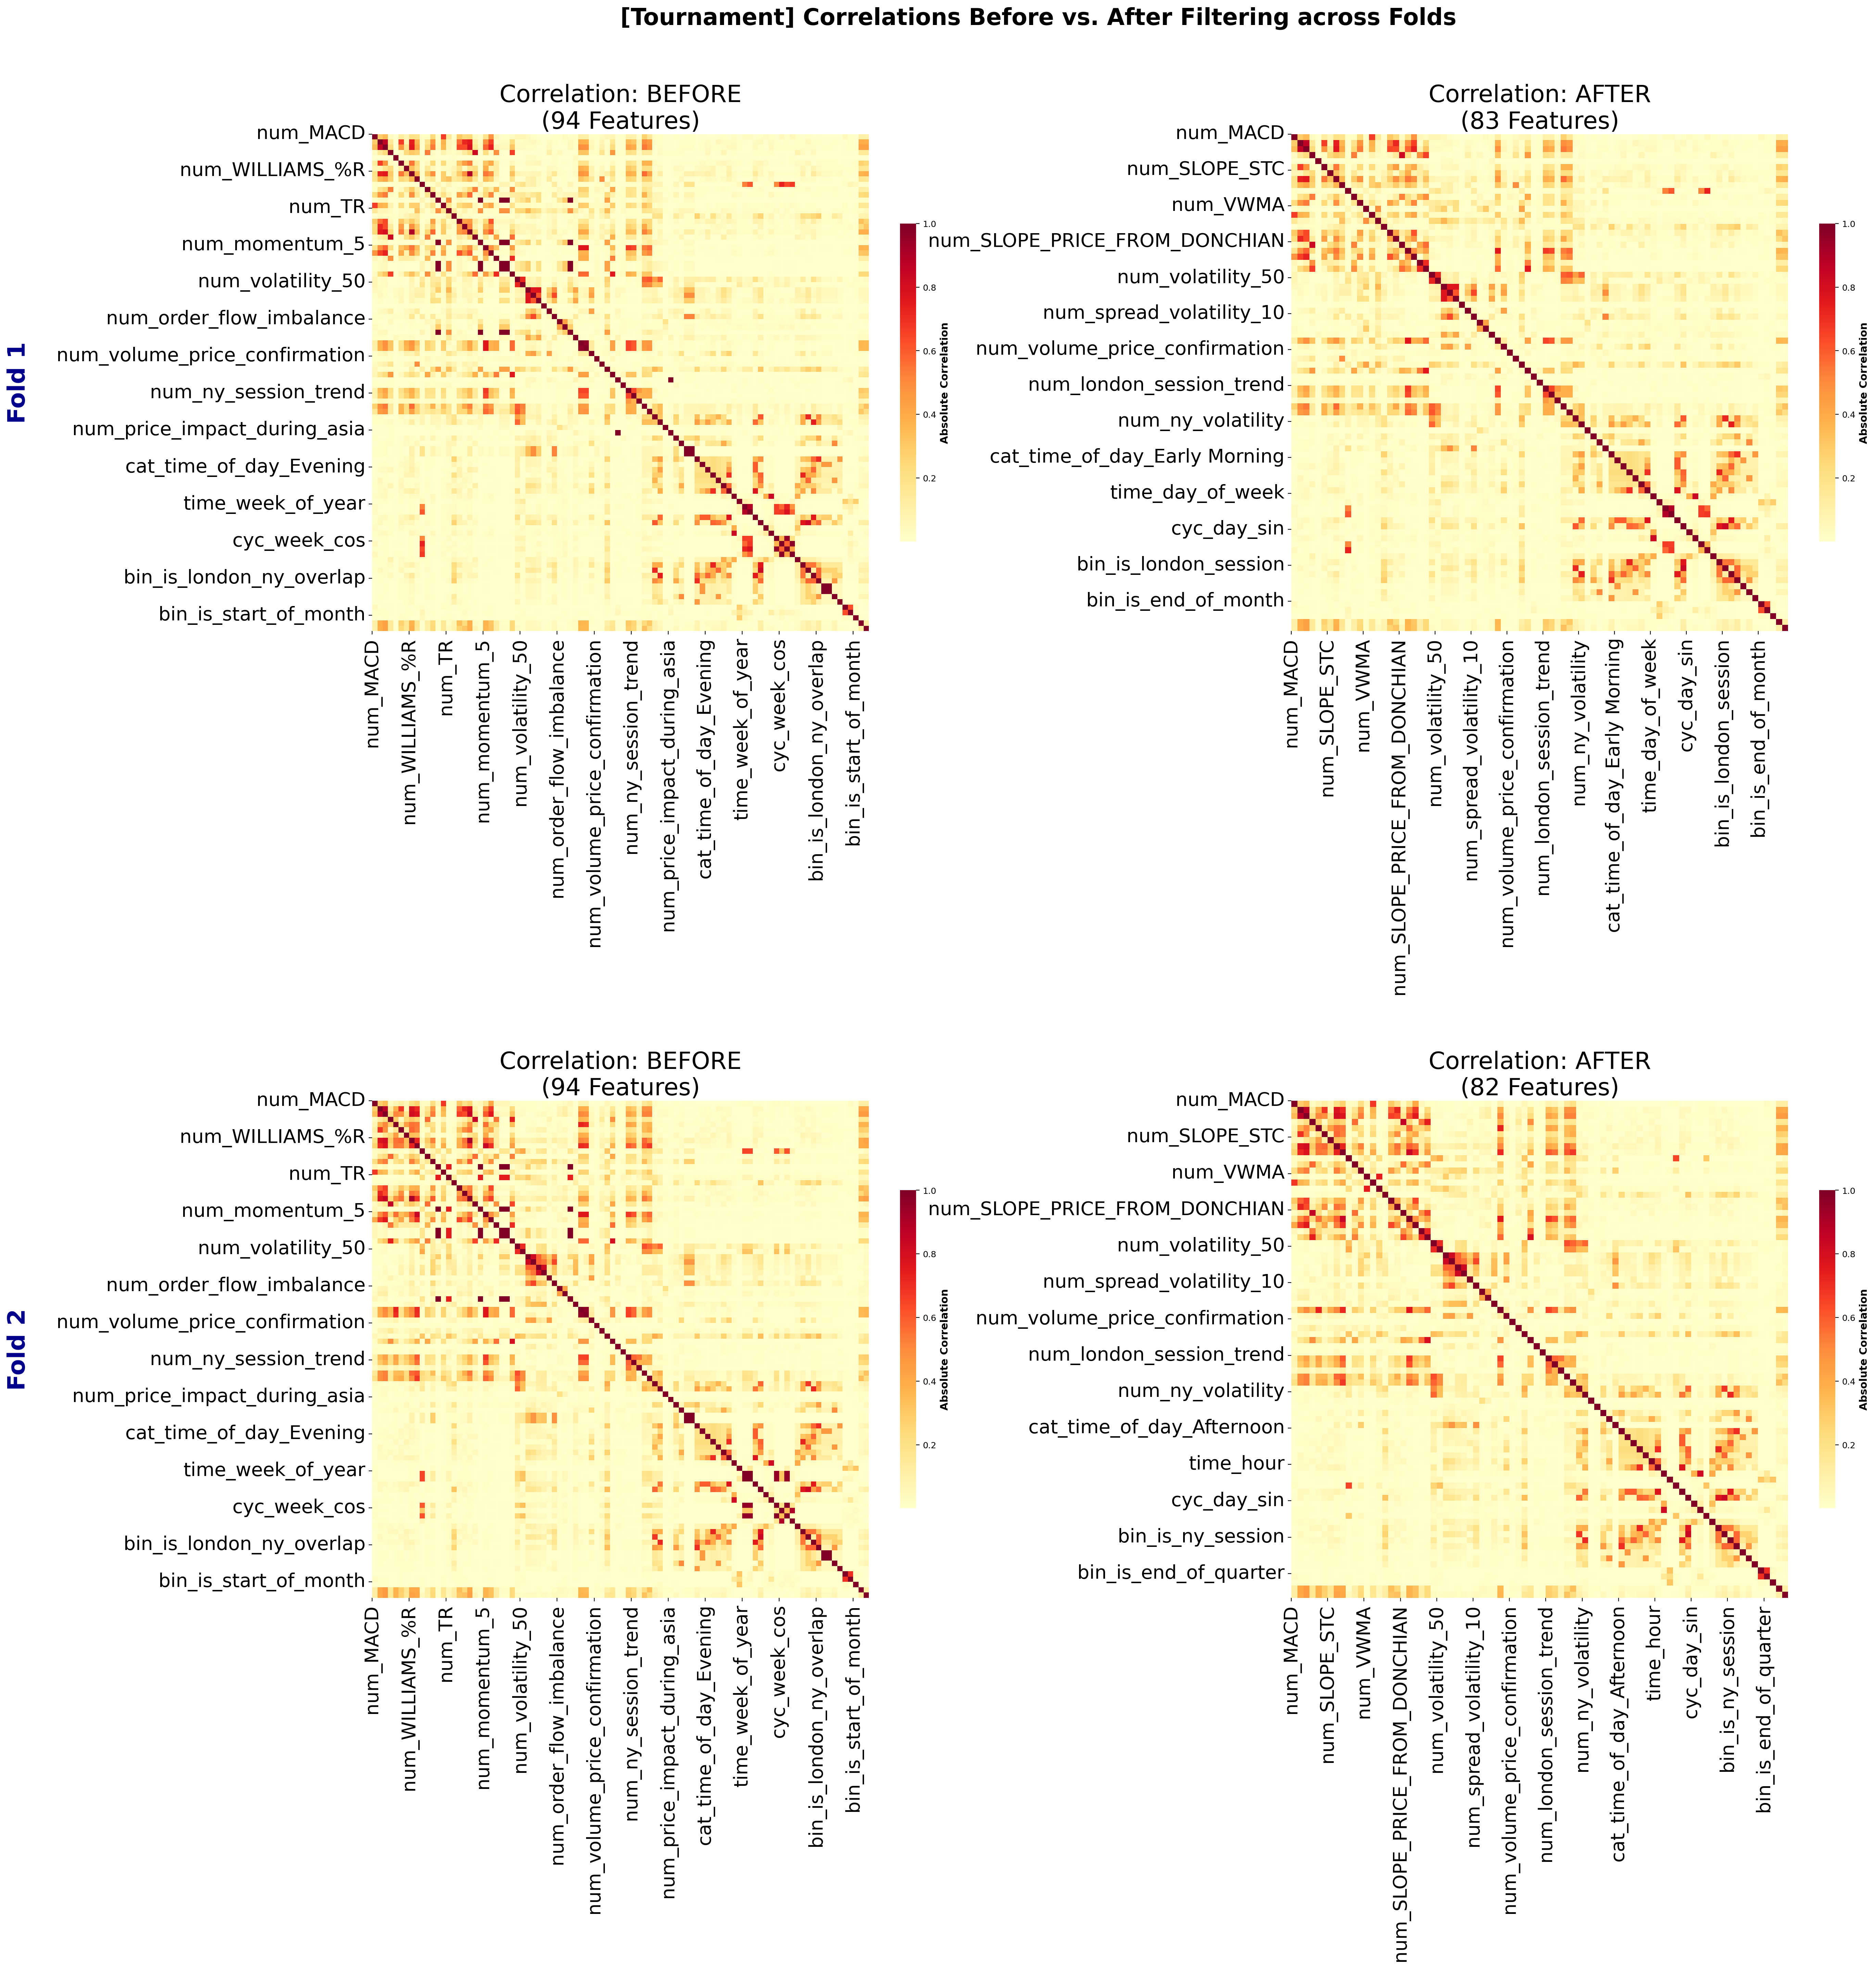
\includegraphics[width=0.9\linewidth]{../data/figures/feature_selection/Tournament_nested_correlation_heatmap.png}
    \caption{Correlation Filtering During Tournament}
    \label{fig:correlation filtering}
\end{figure}


\subsection{Pair- and Model-Specific Parameter Discovery}
\begin{sidewaystable}
\centering
\caption{{Optimized Per-Pair Trading Hyperparameters ExtraTrees (Tournament Phase)}}
\label{tab:hps_ExtraTrees_tournament}
\resizebox{\textwidth}{!}{\begin{tabular}{llllllllll}
\toprule
Fold & Pair & sl mult & tp mult & risk pct & kelly fraction & mh & max notional exposure pct & meta significance & Interpretation \\
\midrule
Fold 1 & AUDUSD & 1.85 & 1.15 & 0.02 & 0.89 & 12.00 & 81.00 & 0.07 &  \\
 & EURUSD & 4.09 & 4.62 & 0.02 & 0.10 & 39.00 & 68.00 & 0.20 &  \\
 & GBPUSD & 1.88 & 1.80 & 0.0091 & 1.00 & 19.00 & 74.00 & 0.11 &  \\
 & NZDUSD & 2.84 & 3.21 & 0.03 & 0.45 & 12.00 & 50.00 & 0.15 &  \\
 & USDCAD & 3.57 & 2.89 & 0.0098 & 0.86 & 10.00 & 71.00 & 0.04 &  \\
 & USDCHF & 2.42 & 2.43 & 0.03 & 0.13 & 17.00 & 56.00 & 0.13 &  \\
 & USDCNH & 3.46 & 2.75 & 0.03 & 0.79 & 41.00 & 78.00 & 0.05 &  \\
 & USDJPY & 2.67 & 2.74 & 0.01 & 0.66 & 24.00 & 66.00 & 0.13 &  \\
 & USDMXN & 1.36 & 2.88 & 0.01 & 0.80 & 44.00 & 63.00 & 0.14 &  \\
 & USDTRY & 2.97 & 1.53 & 0.02 & 0.63 & 23.00 & 77.00 & 0.15 &  \\
 & USDZAR & 2.15 & 3.68 & 0.01 & 0.40 & 26.00 & 69.00 & 0.14 &  \\
Fold 2 & AUDUSD & 3.92 & 3.99 & 0.0057 & 0.48 & 34.00 & 81.00 & 0.02 &  \\
 & EURUSD & 1.20 & 1.74 & 0.02 & 0.37 & 18.00 & 99.00 & 0.08 &  \\
 & GBPUSD & 5.00 & 1.06 & 0.02 & 0.74 & 42.00 & 98.00 & 0.14 &  \\
 & NZDUSD & 1.68 & 1.98 & 0.0050 & 0.84 & 50.00 & 85.00 & 0.19 &  \\
 & USDCAD & 1.87 & 1.88 & 0.03 & 0.10 & 49.00 & 69.00 & 0.20 &  \\
 & USDCHF & 3.34 & 3.80 & 0.0094 & 0.53 & 15.00 & 80.00 & 0.03 &  \\
 & USDCNH & 3.74 & 3.50 & 0.02 & 0.68 & 18.00 & 76.00 & 0.10 &  \\
 & USDJPY & 2.05 & 1.11 & 0.01 & 0.80 & 13.00 & 50.00 & 0.06 &  \\
 & USDMXN & 3.64 & 1.62 & 0.01 & 0.24 & 40.00 & 52.00 & 0.15 &  \\
 & USDTRY & 3.85 & 4.02 & 0.02 & 0.10 & 17.00 & 70.00 & 0.14 &  \\
 & USDZAR & 1.09 & 1.27 & 0.03 & 0.66 & 33.00 & 71.00 & 0.08 &  \\
\bottomrule
\end{tabular}}
\end{sidewaystable}

\begin{table}[H]
\centering
\caption{Hyperparameters for GRU Model (Tournament Phase)}
\label{tab:hps_GRU_tournament}
\begin{tabular}{lccccccccccc}
\toprule
 & \rot{AUDUSD} & \rot{EURUSD} & \rot{GBPUSD} & \rot{NZDUSD} & \rot{USDCAD} & \rot{USDCHF} & \rot{USDCNH} & \rot{USDJPY} & \rot{USDMXN} & \rot{USDTRY} & \rot{USDZAR} \\
\midrule
\multicolumn{11}{c}{\textbf{Fold 1}} \\
\midrule
Kelly F. & 0.86 & 0.43 & 0.88 & 0.76 & 0.32 & 0.47 & 0.11 & 0.77 & 0.86 & 0.67 & 0.10 \\
MH & 41.00 & 18.00 & 26.00 & 49.00 & 20.00 & 42.00 & 19.00 & 28.00 & 33.00 & 18.00 & 31.00 \\
Max Exp. & 100.00 & 62.00 & 86.00 & 79.00 & 100.00 & 73.00 & 61.00 & 92.00 & 93.00 & 62.00 & 83.00 \\
Meta Sig. & 0.04 & 0.05 & 0.17 & 0.05 & 0.07 & 0.02 & 0.08 & 0.14 & 0.03 & 0.09 & 0.11 \\
Risk Pct. & 0.02 & 0.03 & 0.01 & 0.03 & 0.02 & 0.01 & 0.03 & 0.0073 & 0.03 & 0.02 & 0.01 \\
SL Mult. & 1.28 & 1.25 & 4.46 & 3.43 & 2.55 & 4.95 & 3.66 & 2.42 & 4.16 & 2.44 & 3.32 \\
TP Mult. & 3.44 & 1.95 & 2.31 & 3.70 & 2.51 & 1.78 & 4.33 & 2.76 & 2.31 & 1.07 & 1.63 \\
\midrule
\multicolumn{11}{c}{\textbf{Fold 2}} \\
\midrule
Kelly F. & 0.69 & 0.18 & 0.75 & 0.82 & 0.17 & 0.94 & 0.33 & 0.71 & 0.87 & 0.90 & 0.97 \\
MH & 49.00 & 8.00 & 10.00 & 12.00 & 50.00 & 44.00 & 28.00 & 45.00 & 20.00 & 7.00 & 13.00 \\
Max Exp. & 78.00 & 83.00 & 78.00 & 96.00 & 98.00 & 94.00 & 75.00 & 67.00 & 65.00 & 88.00 & 73.00 \\
Meta Sig. & 0.09 & 0.08 & 0.16 & 0.15 & 0.09 & 0.05 & 0.14 & 0.03 & 0.14 & 0.17 & 0.13 \\
Risk Pct. & 0.02 & 0.01 & 0.02 & 0.02 & 0.02 & 0.01 & 0.02 & 0.01 & 0.01 & 0.02 & 0.02 \\
SL Mult. & 1.97 & 4.97 & 1.98 & 3.30 & 4.85 & 4.83 & 4.01 & 1.02 & 1.71 & 2.05 & 1.21 \\
TP Mult. & 3.29 & 2.19 & 3.27 & 3.26 & 1.37 & 4.67 & 2.50 & 3.48 & 2.29 & 1.08 & 3.10 \\
\bottomrule
\end{tabular}
\end{table}
\begin{table}[H]
\centering
\caption{Hyperparameters for LightGBM Model (Tournament Phase)}
\label{tab:hps_LightGBM_tournament}
\resizebox{\textwidth}{!}{%
\begin{tabular}{lccccccccccc}
\toprule
 & \rot{AUDUSD} & \rot{EURUSD} & \rot{GBPUSD} & \rot{NZDUSD} & \rot{USDCAD} & \rot{USDCHF} & \rot{USDCNH} & \rot{USDJPY} & \rot{USDMXN} & \rot{USDTRY} & \rot{USDZAR} \\
\midrule
\multicolumn{11}{c}{\textbf{Fold 1}} \\
\midrule
Kelly F. & 1.00 & 0.78 & 0.50 & 0.16 & 0.81 & 0.76 & 0.42 & 0.97 & 0.40 & 0.26 & 0.25 \\
MH & 48.00 & 25.00 & 50.00 & 42.00 & 5.00 & 21.00 & 18.00 & 30.00 & 26.00 & 11.00 & 42.00 \\
Max Exp. & 98.00 & 83.00 & 66.00 & 95.00 & 61.00 & 87.00 & 72.00 & 91.00 & 87.00 & 77.00 & 99.00 \\
Meta Sig. & 0.07 & 0.01 & 0.09 & 0.04 & 0.09 & 0.09 & 0.20 & 0.13 & 0.01 & 0.05 & 0.15 \\
Risk Pct. & 0.03 & 0.01 & 0.02 & 0.02 & 0.03 & 0.03 & 0.02 & 0.02 & 0.03 & 0.03 & 0.01 \\
SL Mult. & 3.81 & 3.12 & 4.90 & 4.33 & 1.10 & 1.66 & 1.33 & 2.55 & 1.97 & 3.27 & 2.24 \\
TP Mult. & 2.89 & 1.01 & 3.50 & 4.81 & 3.46 & 4.37 & 5.00 & 4.23 & 4.97 & 2.87 & 3.50 \\
\midrule
\multicolumn{11}{c}{\textbf{Fold 2}} \\
\midrule
Kelly F. & 0.41 & 0.80 & 0.54 & 0.90 & 0.67 & 0.22 & 0.49 & 0.70 & 0.35 & 0.24 & 0.75 \\
MH & 38.00 & 36.00 & 36.00 & 5.00 & 49.00 & 32.00 & 50.00 & 50.00 & 5.00 & 11.00 & 33.00 \\
Max Exp. & 65.00 & 100.00 & 90.00 & 84.00 & 51.00 & 77.00 & 69.00 & 82.00 & 62.00 & 89.00 & 53.00 \\
Meta Sig. & 0.04 & 0.16 & 0.08 & 0.19 & 0.08 & 0.18 & 0.08 & 0.17 & 0.13 & 0.01 & 0.19 \\
Risk Pct. & 0.01 & 0.02 & 0.02 & 0.0058 & 0.02 & 0.0080 & 0.02 & 0.02 & 0.02 & 0.03 & 0.01 \\
SL Mult. & 4.20 & 1.27 & 3.92 & 2.48 & 4.97 & 2.78 & 2.18 & 4.85 & 2.14 & 3.39 & 1.83 \\
TP Mult. & 3.43 & 4.22 & 3.06 & 1.44 & 2.17 & 4.01 & 4.08 & 1.07 & 4.03 & 3.82 & 4.02 \\
\bottomrule
\end{tabular}
}%
\end{table}
\begin{table}[H]
\centering
\caption{Hyperparameters for LSTM Model (Tournament Phase)}
\label{tab:hps_LSTM_tournament}
\resizebox{\textwidth}{!}{%
\begin{tabular}{lccccccccccc}
\toprule
 & \rot{AUDUSD} & \rot{EURUSD} & \rot{GBPUSD} & \rot{NZDUSD} & \rot{USDCAD} & \rot{USDCHF} & \rot{USDCNH} & \rot{USDJPY} & \rot{USDMXN} & \rot{USDTRY} & \rot{USDZAR} \\
\midrule
\multicolumn{11}{c}{\textbf{Fold 1}} \\
\midrule
Kelly F. & 1.00 & 0.29 & 0.19 & 0.55 & 0.58 & 0.13 & 0.60 & 0.85 & 0.24 & 0.50 & 0.59 \\
MH & 20.00 & 20.00 & 5.00 & 35.00 & 44.00 & 20.00 & 29.00 & 50.00 & 20.00 & 32.00 & 18.00 \\
Max Exp. & 71.00 & 56.00 & 90.00 & 88.00 & 76.00 & 65.00 & 57.00 & 82.00 & 51.00 & 59.00 & 70.00 \\
Meta Sig. & 0.08 & 0.05 & 0.12 & 0.13 & 0.17 & 0.13 & 0.13 & 0.04 & 0.03 & 0.12 & 0.08 \\
Risk Pct. & 0.02 & 0.0086 & 0.02 & 0.02 & 0.02 & 0.01 & 0.01 & 0.02 & 0.0064 & 0.0090 & 0.01 \\
SL Mult. & 4.67 & 2.71 & 4.13 & 3.65 & 3.26 & 1.62 & 2.88 & 3.52 & 1.66 & 2.19 & 2.40 \\
TP Mult. & 3.53 & 3.37 & 2.48 & 2.02 & 4.31 & 1.81 & 2.76 & 3.23 & 1.42 & 2.90 & 2.40 \\
\midrule
\multicolumn{11}{c}{\textbf{Fold 2}} \\
\midrule
Kelly F. & 0.18 & 0.34 & 0.97 & 0.91 & 0.11 & 0.44 & 0.15 & 0.22 & 0.11 & 0.63 & 0.89 \\
MH & 24.00 & 6.00 & 49.00 & 39.00 & 35.00 & 30.00 & 6.00 & 7.00 & 23.00 & 31.00 & 5.00 \\
Max Exp. & 52.00 & 100.00 & 51.00 & 66.00 & 72.00 & 66.00 & 100.00 & 72.00 & 50.00 & 68.00 & 68.00 \\
Meta Sig. & 0.01 & 0.20 & 0.13 & 0.11 & 0.12 & 0.20 & 0.19 & 0.09 & 0.13 & 0.02 & 0.12 \\
Risk Pct. & 0.02 & 0.02 & 0.02 & 0.01 & 0.03 & 0.03 & 0.03 & 0.02 & 0.0051 & 0.02 & 0.01 \\
SL Mult. & 1.49 & 5.00 & 1.10 & 3.13 & 1.31 & 3.80 & 4.80 & 1.21 & 4.91 & 1.08 & 1.11 \\
TP Mult. & 3.25 & 4.16 & 1.02 & 1.06 & 1.02 & 4.92 & 2.25 & 3.63 & 4.34 & 2.20 & 3.37 \\
\bottomrule
\end{tabular}
}%
\end{table}
\begin{table}[H]
\centering
\caption{Hyperparameters for RandomForest Model (Tournament Phase)}
\label{tab:hps_RandomForest_tournament}
\resizebox{\textwidth}{!}{%
\begin{tabular}{lccccccccccc}
\toprule
 & \rot{AUDUSD} & \rot{EURUSD} & \rot{GBPUSD} & \rot{NZDUSD} & \rot{USDCAD} & \rot{USDCHF} & \rot{USDCNH} & \rot{USDJPY} & \rot{USDMXN} & \rot{USDTRY} & \rot{USDZAR} \\
\midrule
\multicolumn{11}{c}{\textbf{Fold 1}} \\
\midrule
Kelly F. & 0.60 & 0.88 & 0.93 & 0.42 & 0.65 & 0.33 & 0.41 & 0.13 & 0.28 & 0.10 & 0.63 \\
MH & 21.00 & 25.00 & 26.00 & 38.00 & 33.00 & 7.00 & 24.00 & 26.00 & 48.00 & 25.00 & 37.00 \\
Max Exp. & 94.00 & 87.00 & 62.00 & 67.00 & 80.00 & 71.00 & 88.00 & 82.00 & 98.00 & 79.00 & 73.00 \\
Meta Sig. & 0.14 & 0.20 & 0.10 & 0.01 & 0.19 & 0.11 & 0.12 & 0.10 & 0.16 & 0.17 & 0.19 \\
Risk Pct. & 0.02 & 0.0098 & 0.03 & 0.02 & 0.02 & 0.03 & 0.0087 & 0.03 & 0.01 & 0.03 & 0.0078 \\
SL Mult. & 2.04 & 1.15 & 4.30 & 4.12 & 2.49 & 4.57 & 3.66 & 4.55 & 3.59 & 1.28 & 1.63 \\
TP Mult. & 1.08 & 4.34 & 1.08 & 3.04 & 3.83 & 2.71 & 2.28 & 3.34 & 3.51 & 2.01 & 1.22 \\
\midrule
\multicolumn{11}{c}{\textbf{Fold 2}} \\
\midrule
Kelly F. & 0.94 & 0.65 & 0.30 & 0.60 & 0.37 & 0.14 & 0.66 & 0.39 & 0.14 & 0.99 & 0.99 \\
MH & 49.00 & 47.00 & 44.00 & 28.00 & 40.00 & 17.00 & 21.00 & 5.00 & 36.00 & 14.00 & 5.00 \\
Max Exp. & 73.00 & 62.00 & 65.00 & 62.00 & 66.00 & 67.00 & 73.00 & 61.00 & 57.00 & 70.00 & 100.00 \\
Meta Sig. & 0.12 & 0.13 & 0.12 & 0.19 & 0.14 & 0.02 & 0.13 & 0.10 & 0.08 & 0.08 & 0.12 \\
Risk Pct. & 0.01 & 0.02 & 0.02 & 0.03 & 0.01 & 0.01 & 0.03 & 0.02 & 0.01 & 0.0059 & 0.01 \\
SL Mult. & 4.10 & 3.46 & 1.02 & 4.84 & 3.42 & 4.98 & 4.07 & 3.83 & 3.64 & 1.16 & 3.36 \\
TP Mult. & 2.53 & 3.70 & 4.02 & 2.29 & 2.04 & 4.97 & 2.18 & 1.01 & 2.31 & 1.18 & 3.16 \\
\bottomrule
\end{tabular}
}%
\end{table}

\subsection{Model-Specific Backtest Results}\label{app:model_specific_backtests}
\begin{figure}[H]
    \centering
    \begin{minipage}[t]{0.49\textwidth}
        \centering
        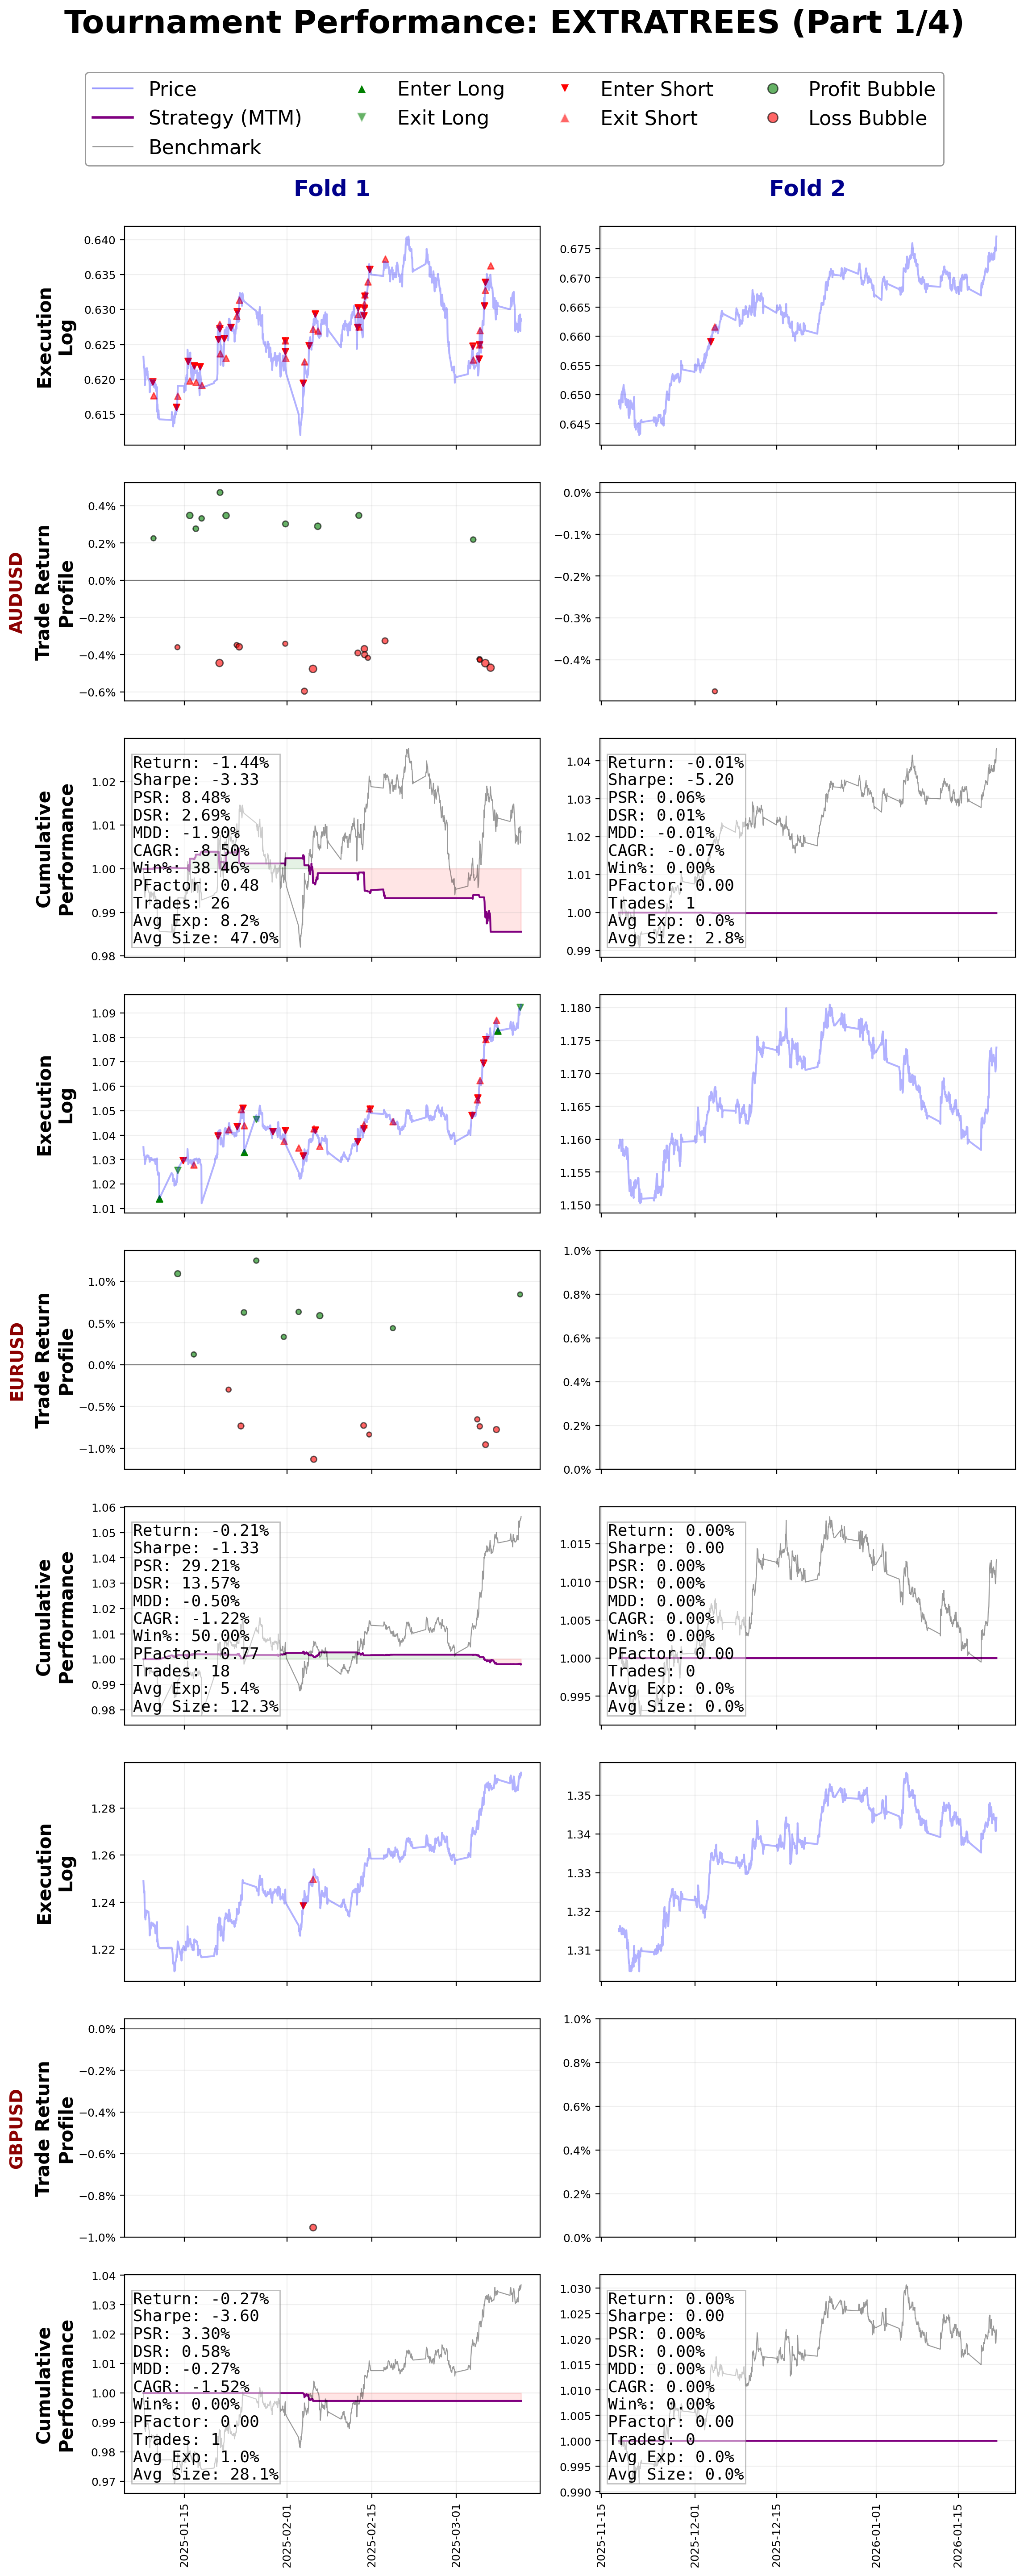
\includegraphics[width=\textwidth]{../data/figures/backtests/tournament_results_ExtraTrees_part1.png}
        \caption{Backtest Result of ExtraTrees During Tournament}
        \label{fig:tournament_results_ExtraTrees_1}
    \end{minipage}
    \hfill
    \begin{minipage}[t]{0.49\textwidth}
        \centering
        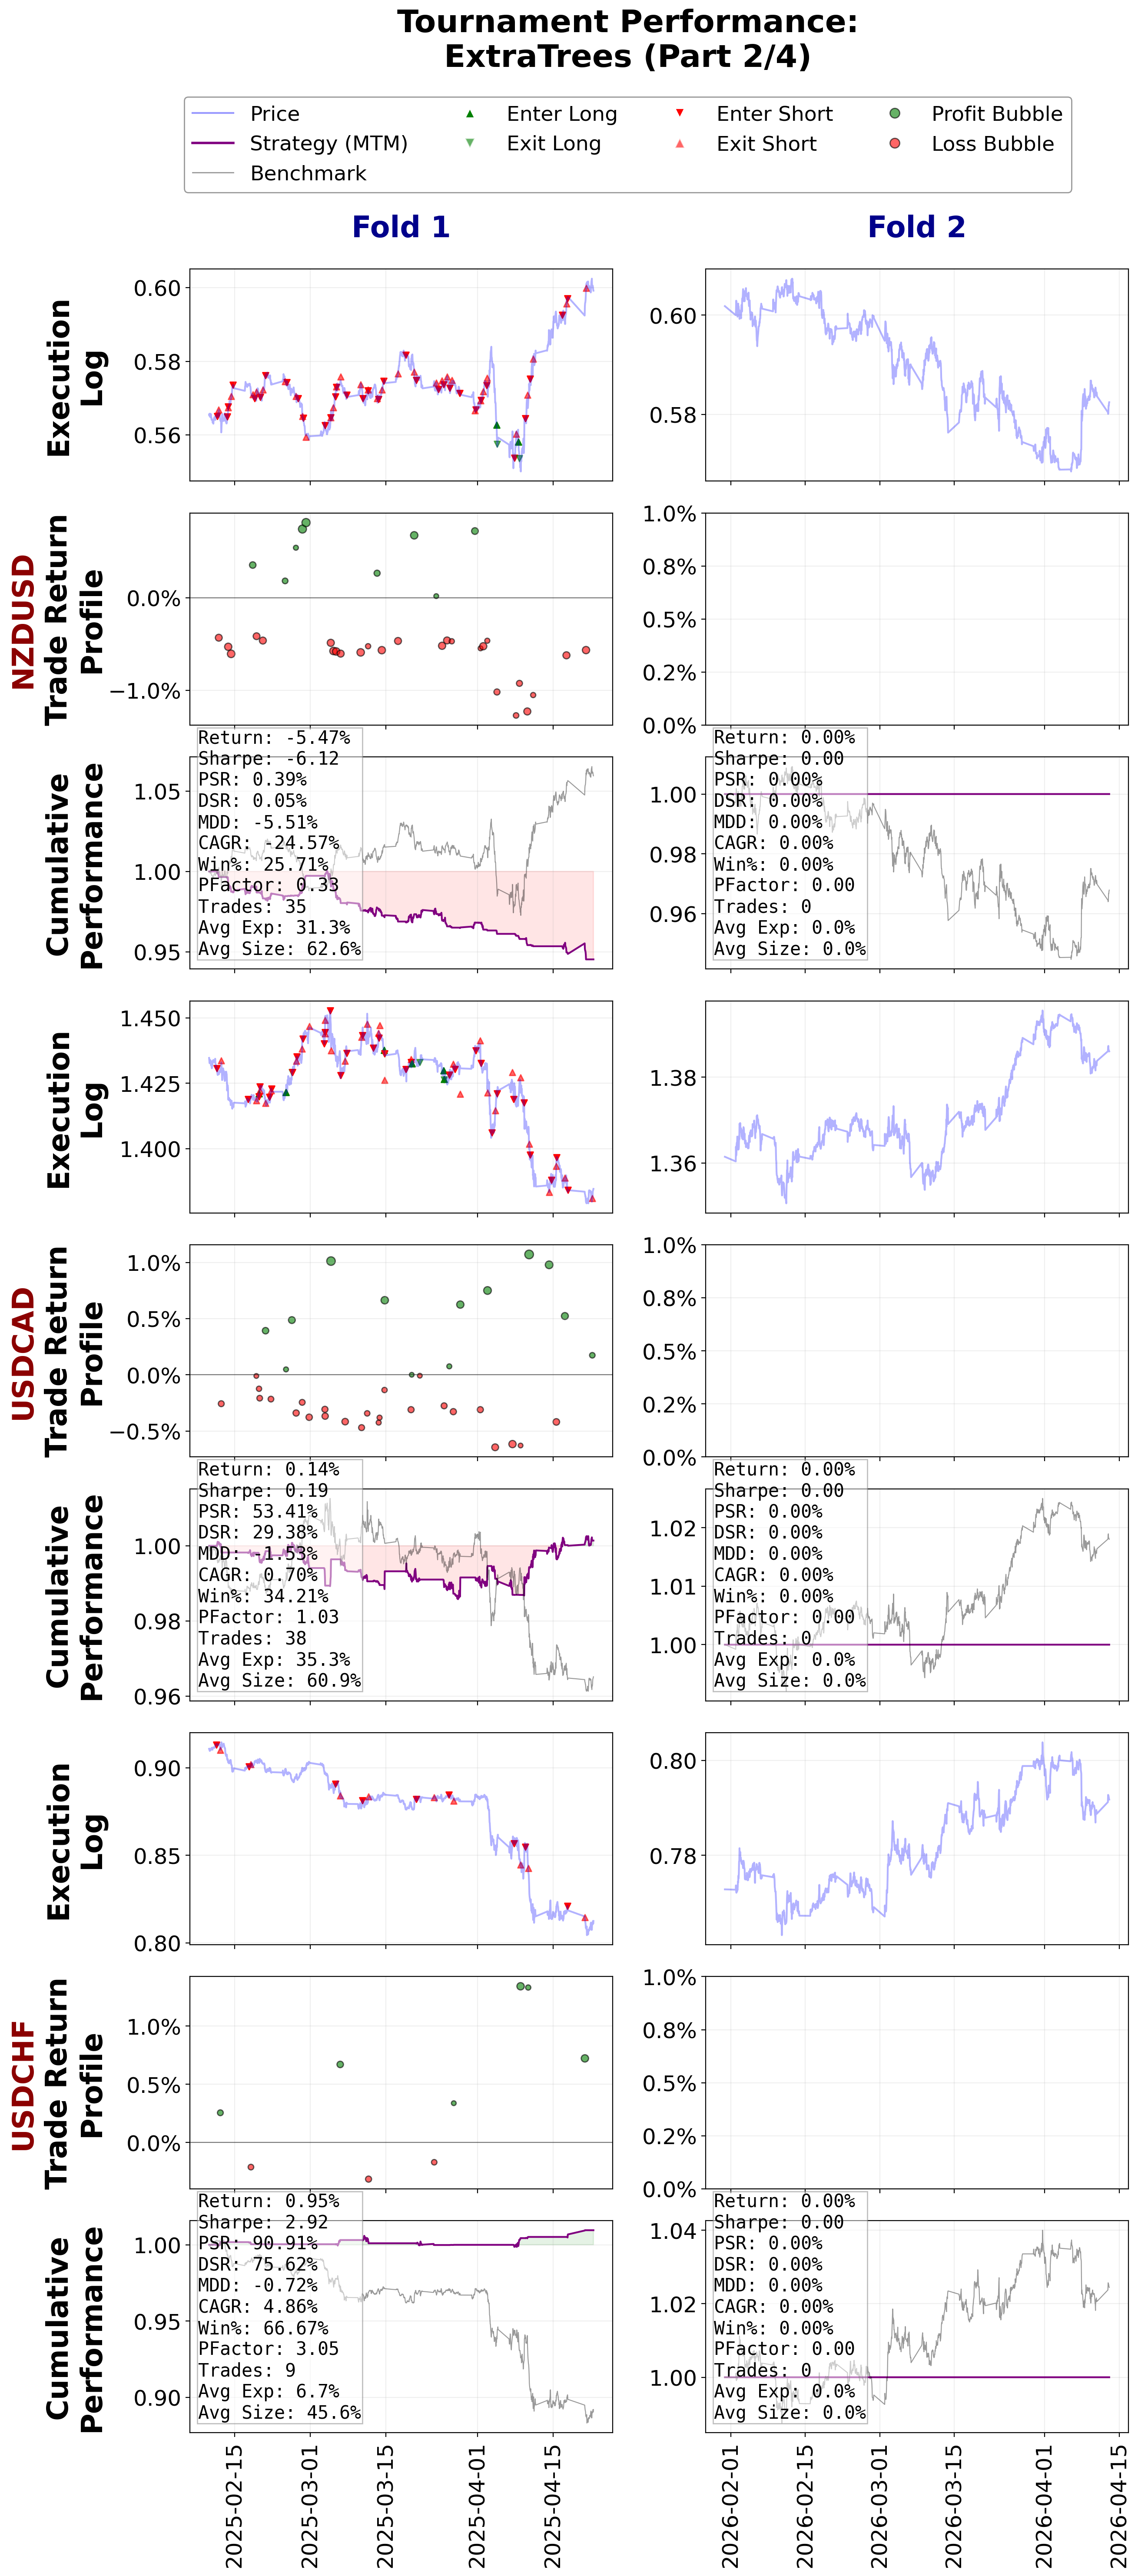
\includegraphics[width=\textwidth]{../data/figures/backtests/tournament_results_ExtraTrees_part2.png}
        \caption{Backtest Result of ExtraTrees During Tournament (Continued)}
        \label{fig:tournament_results_ExtraTrees_2}
    \end{minipage}
\end{figure}

\begin{figure}[H]
    \centering
    \begin{minipage}[t]{0.49\textwidth}
        \centering
        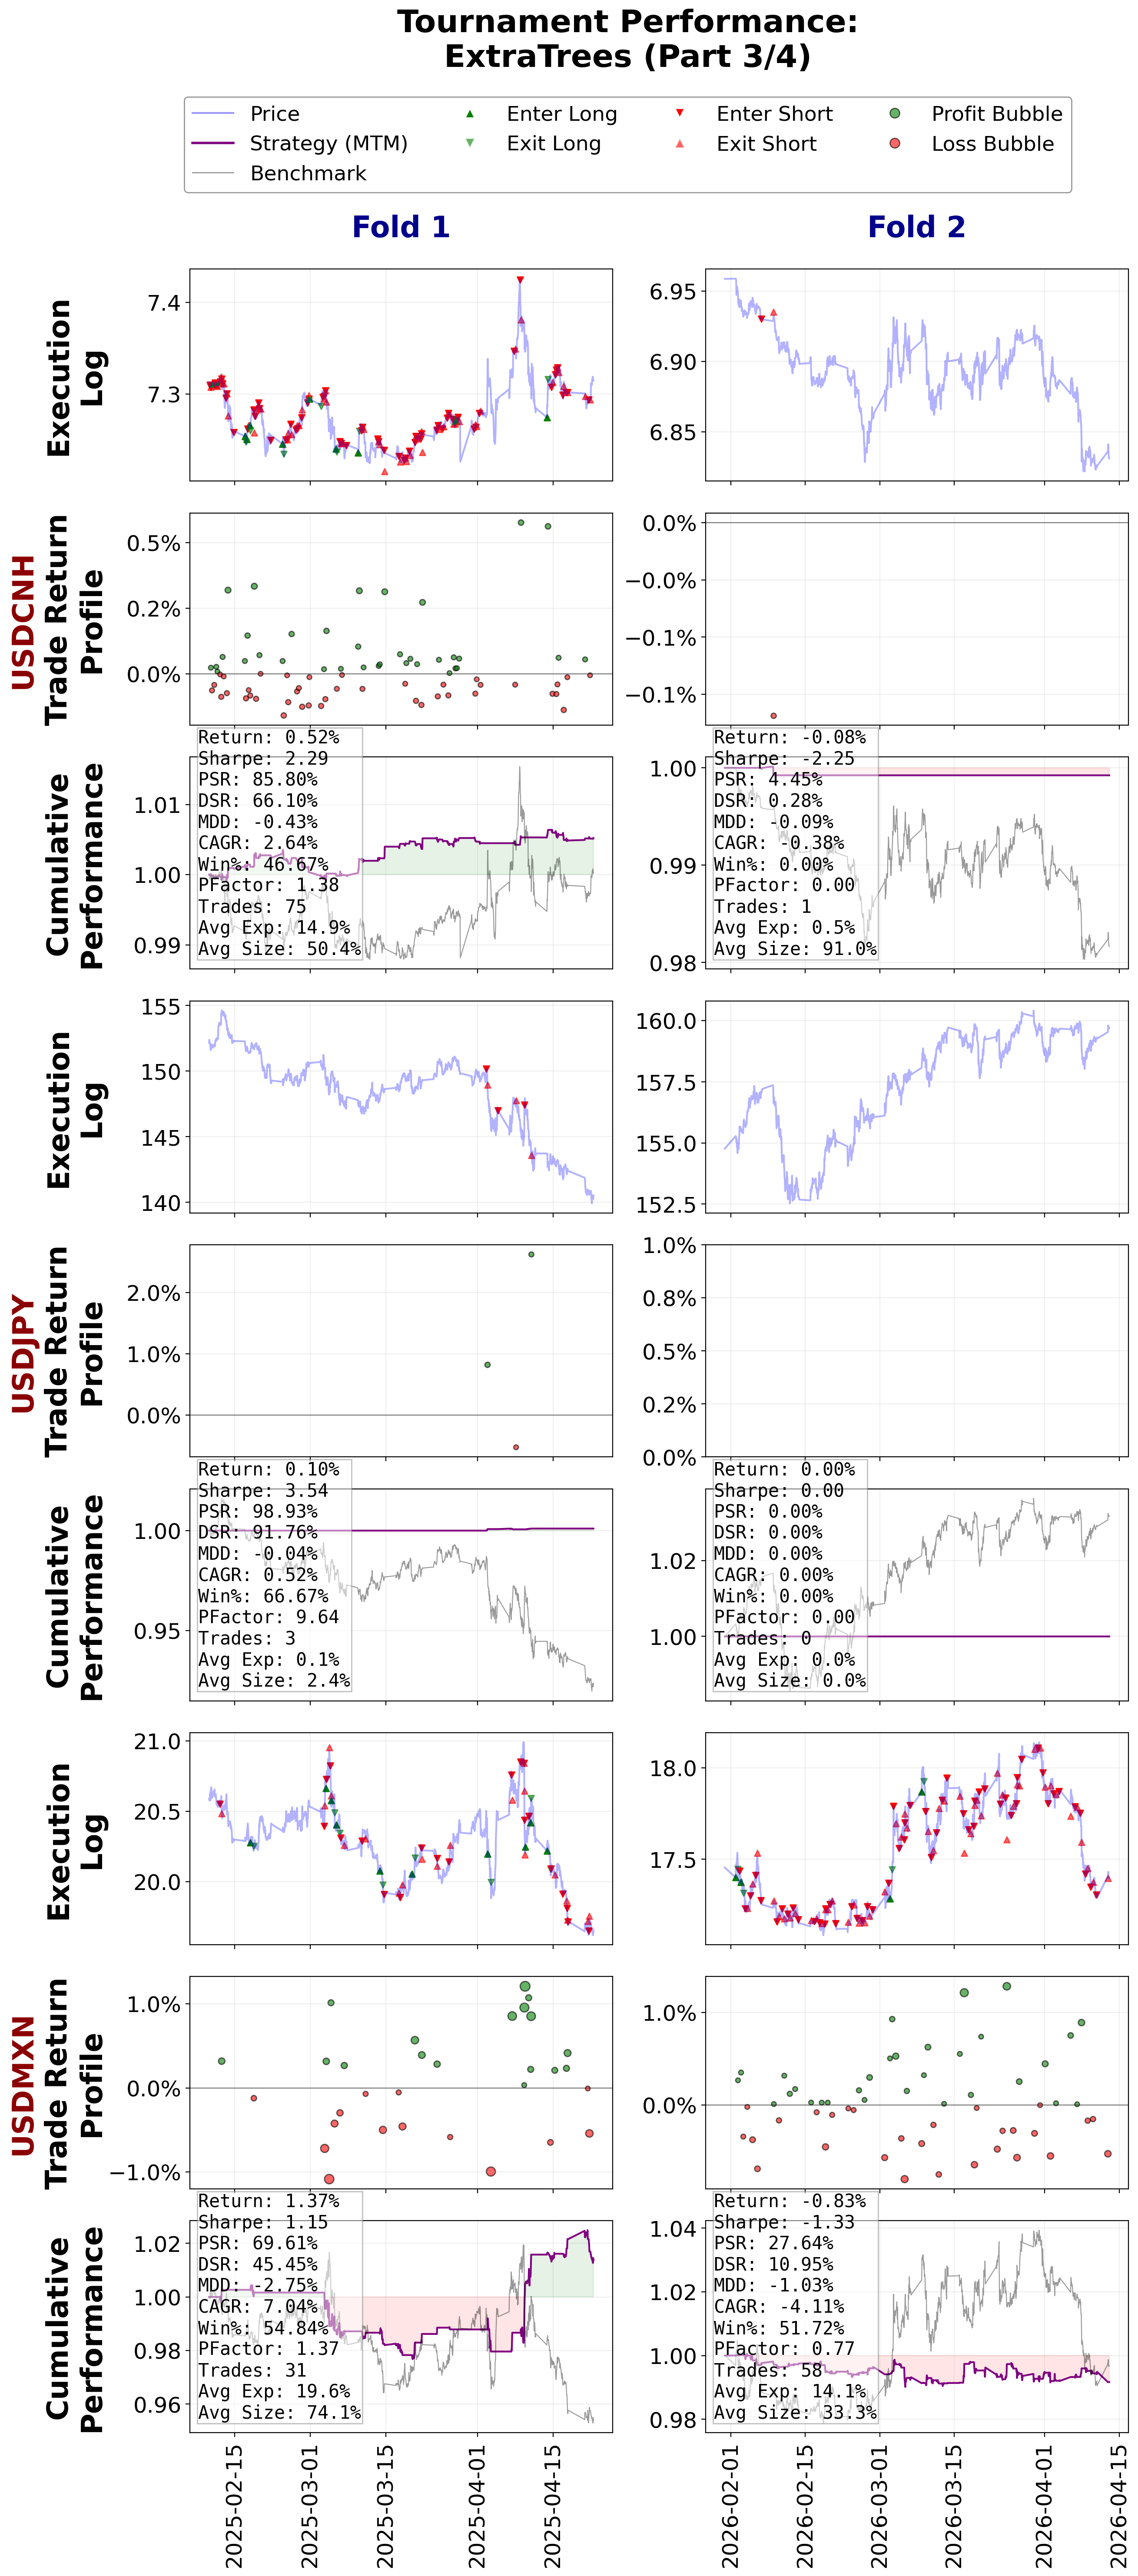
\includegraphics[width=\textwidth]{../data/figures/backtests/tournament_results_ExtraTrees_part3.png}
        \caption{Backtest Result of ExtraTrees During Tournament (Continued)}
        \label{fig:tournament_results_ExtraTrees_3}
    \end{minipage}
    \hfill
    \begin{minipage}[t]{0.49\textwidth}
        \centering
        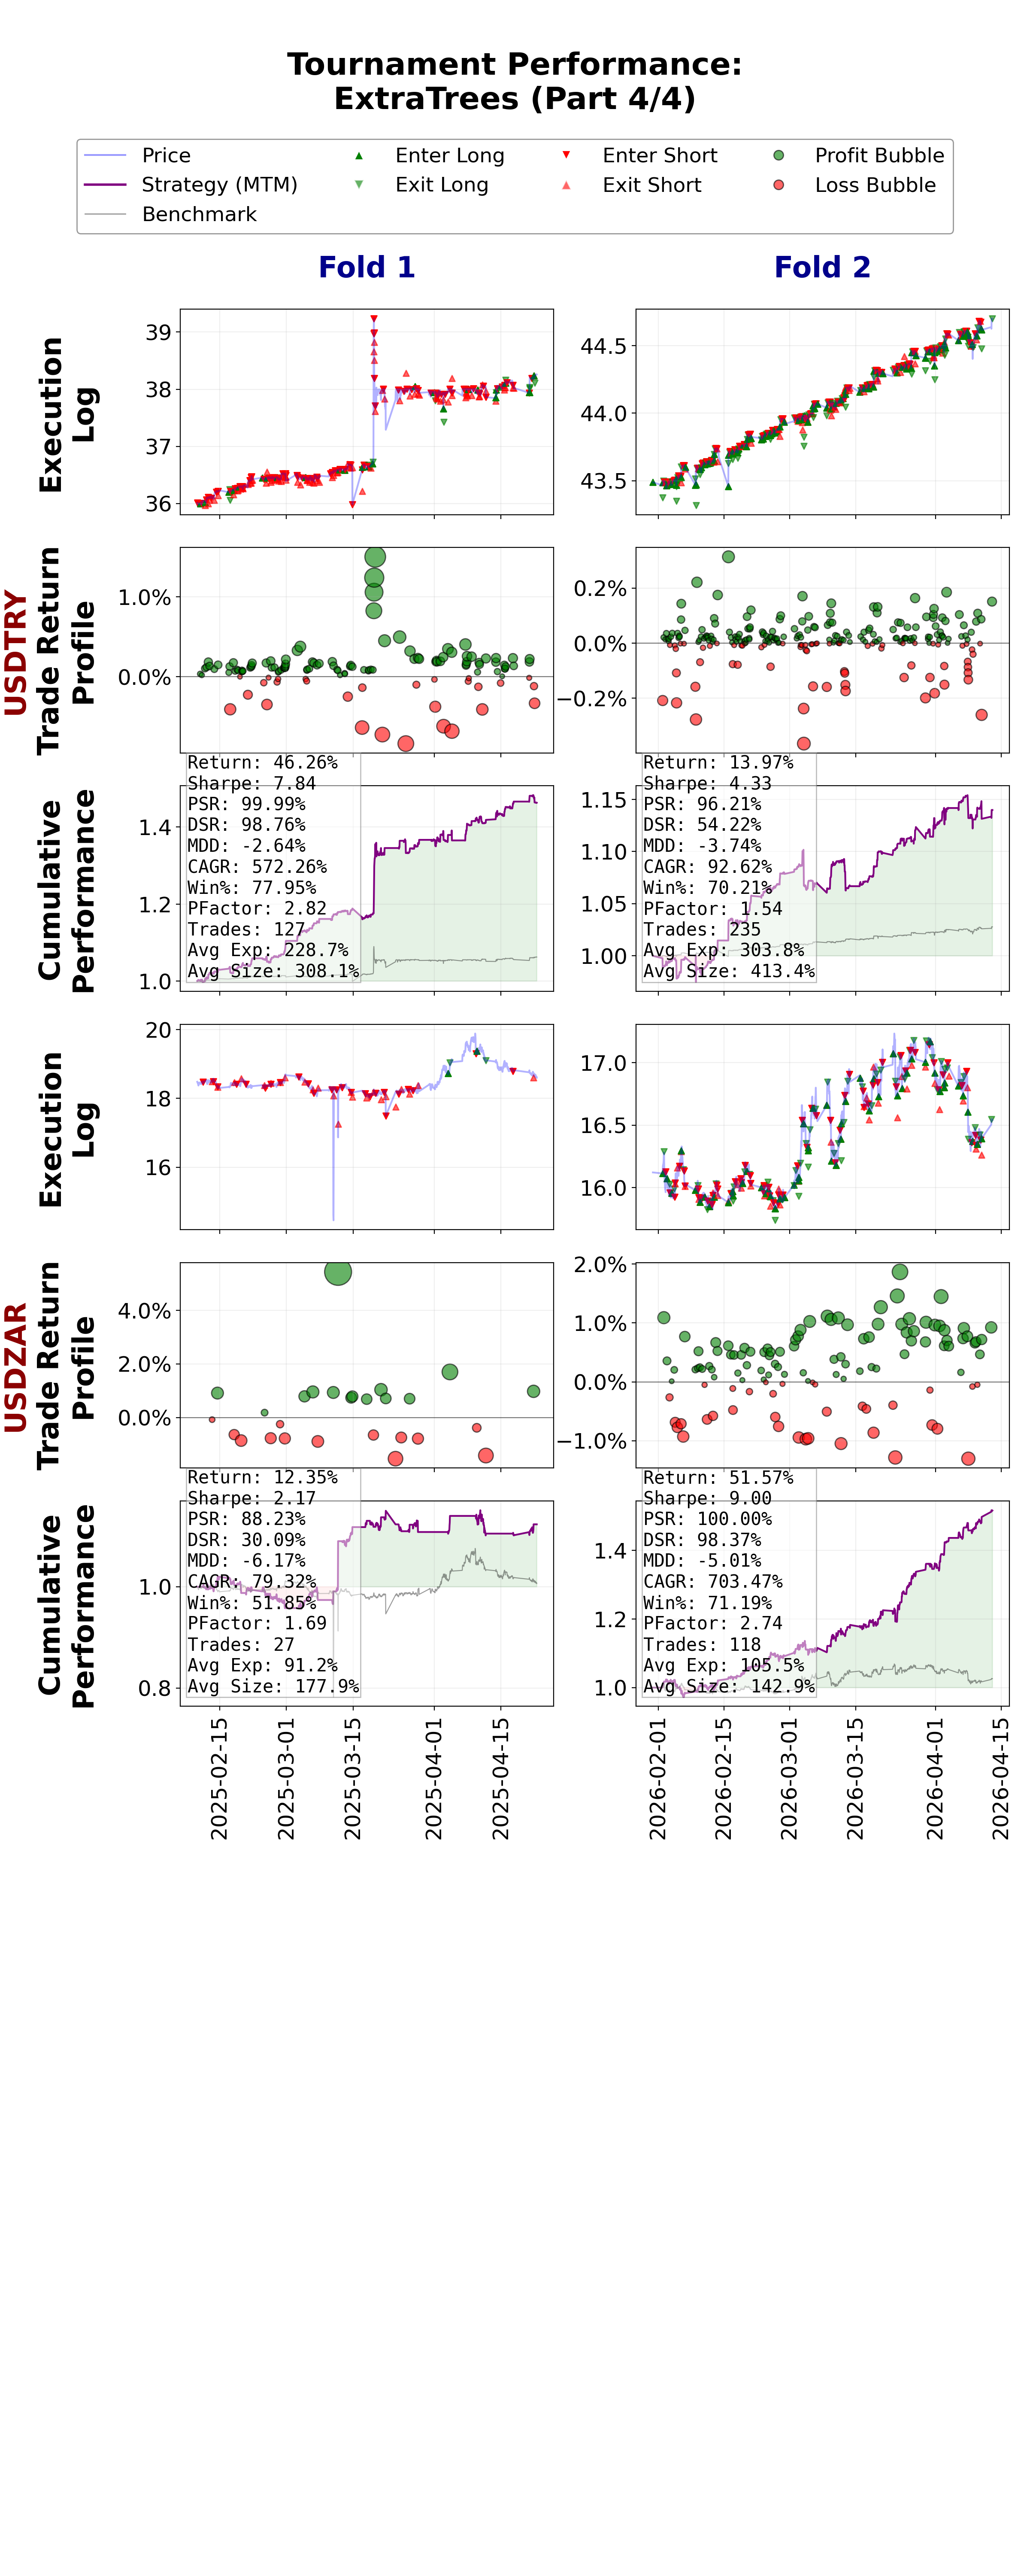
\includegraphics[width=\textwidth]{../data/figures/backtests/tournament_results_ExtraTrees_part4.png}
        \caption{Backtest Result of ExtraTrees During Tournament (Continued)}
        \label{fig:tournament_results_ExtraTrees_4}
    \end{minipage}
\end{figure}


\begin{figure}[H]
    \centering
    \begin{minipage}[t]{0.49\textwidth}
        \centering
        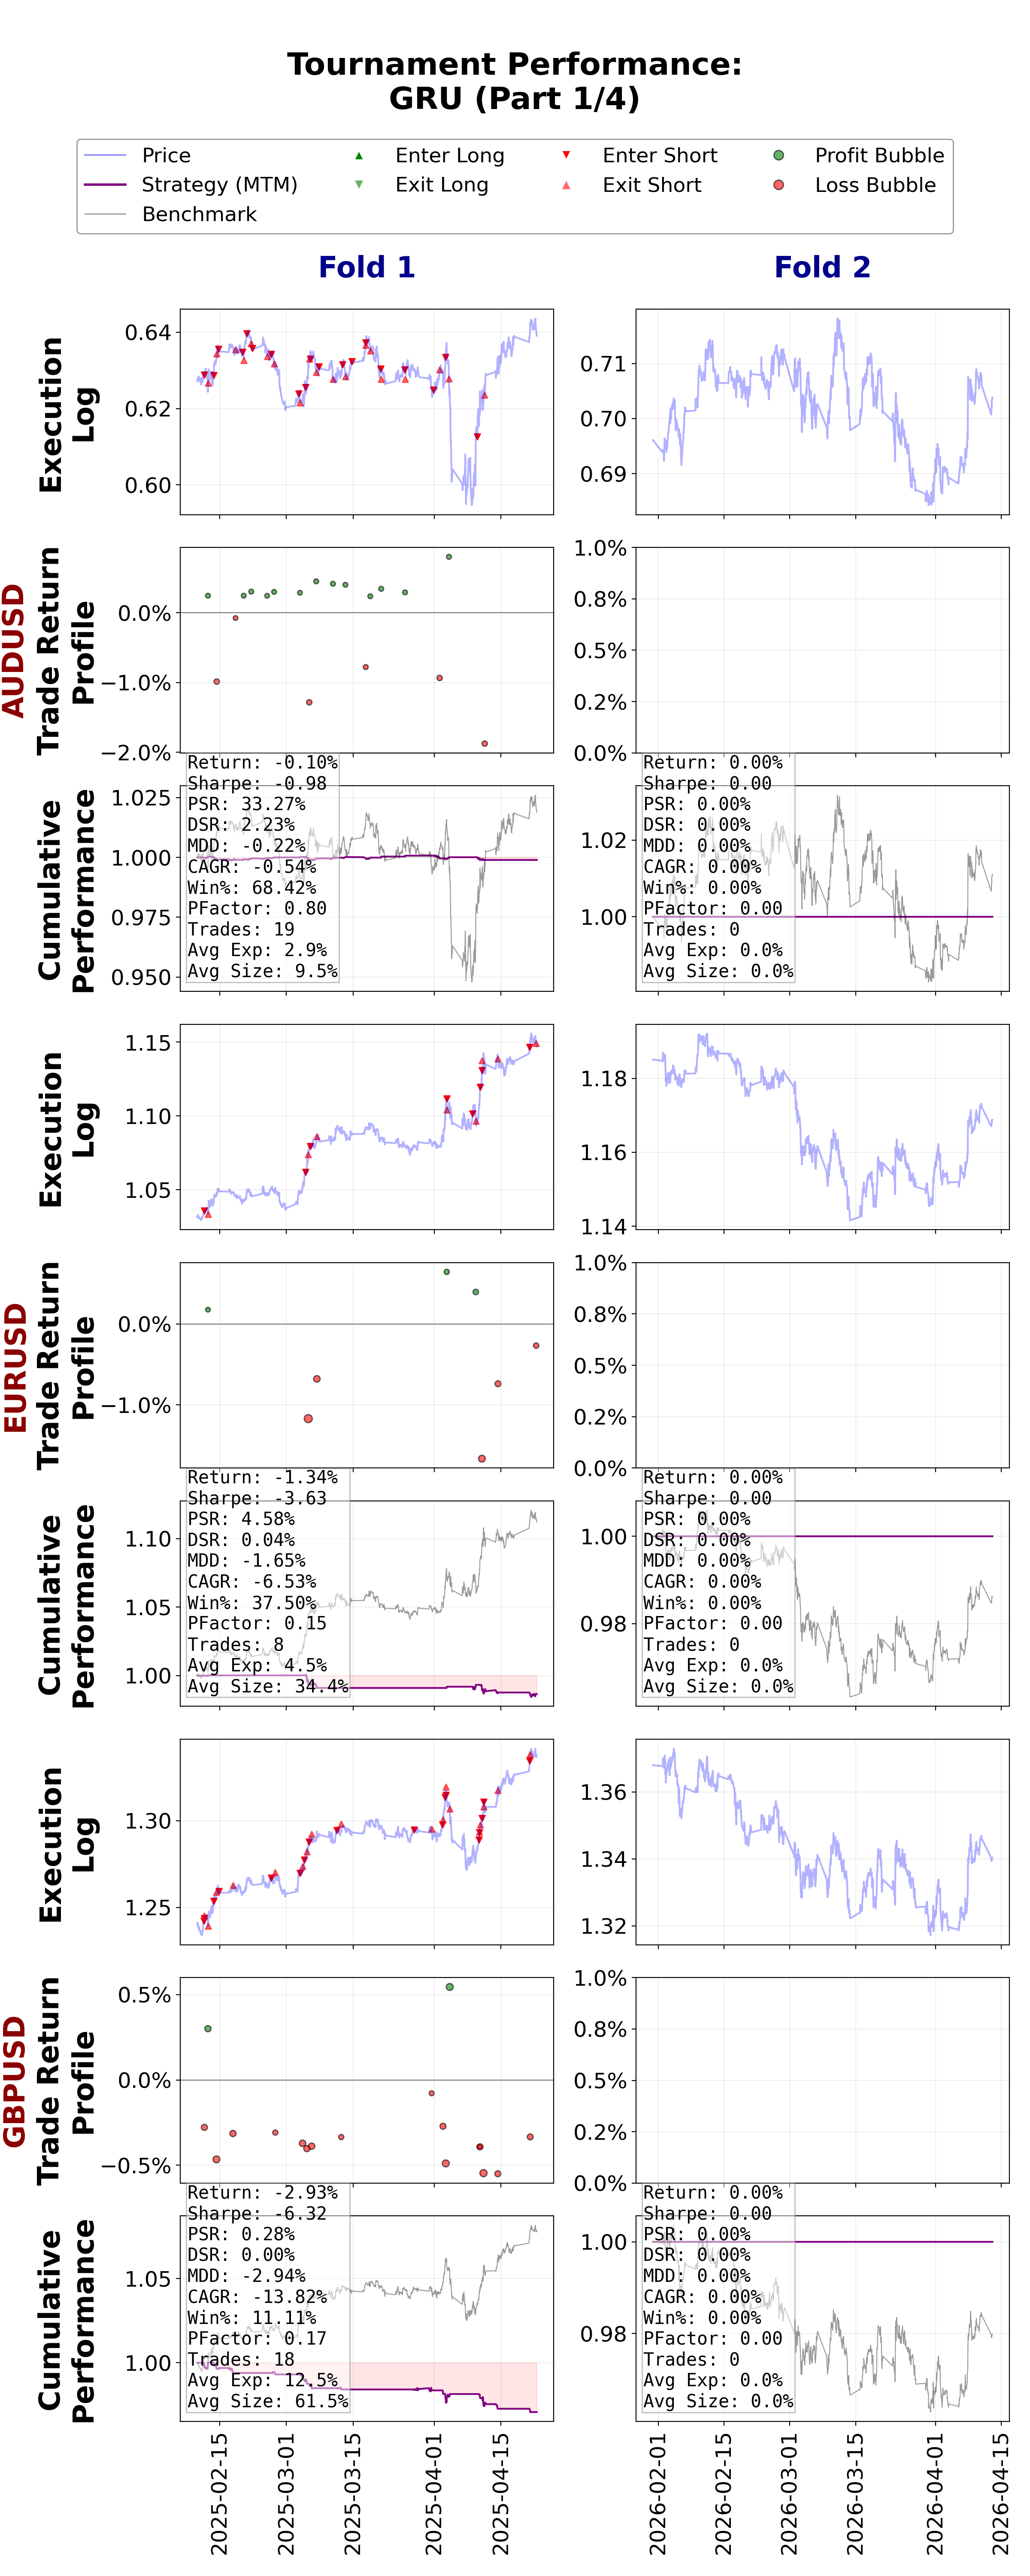
\includegraphics[width=\textwidth]{../data/figures/backtests/tournament_results_GRU_part1.png}
        \caption{Backtest Result of GRU During Tournament}
        \label{fig:tournament_results_GRU_1}
    \end{minipage}
    \hfill
    \begin{minipage}[t]{0.49\textwidth}
        \centering
        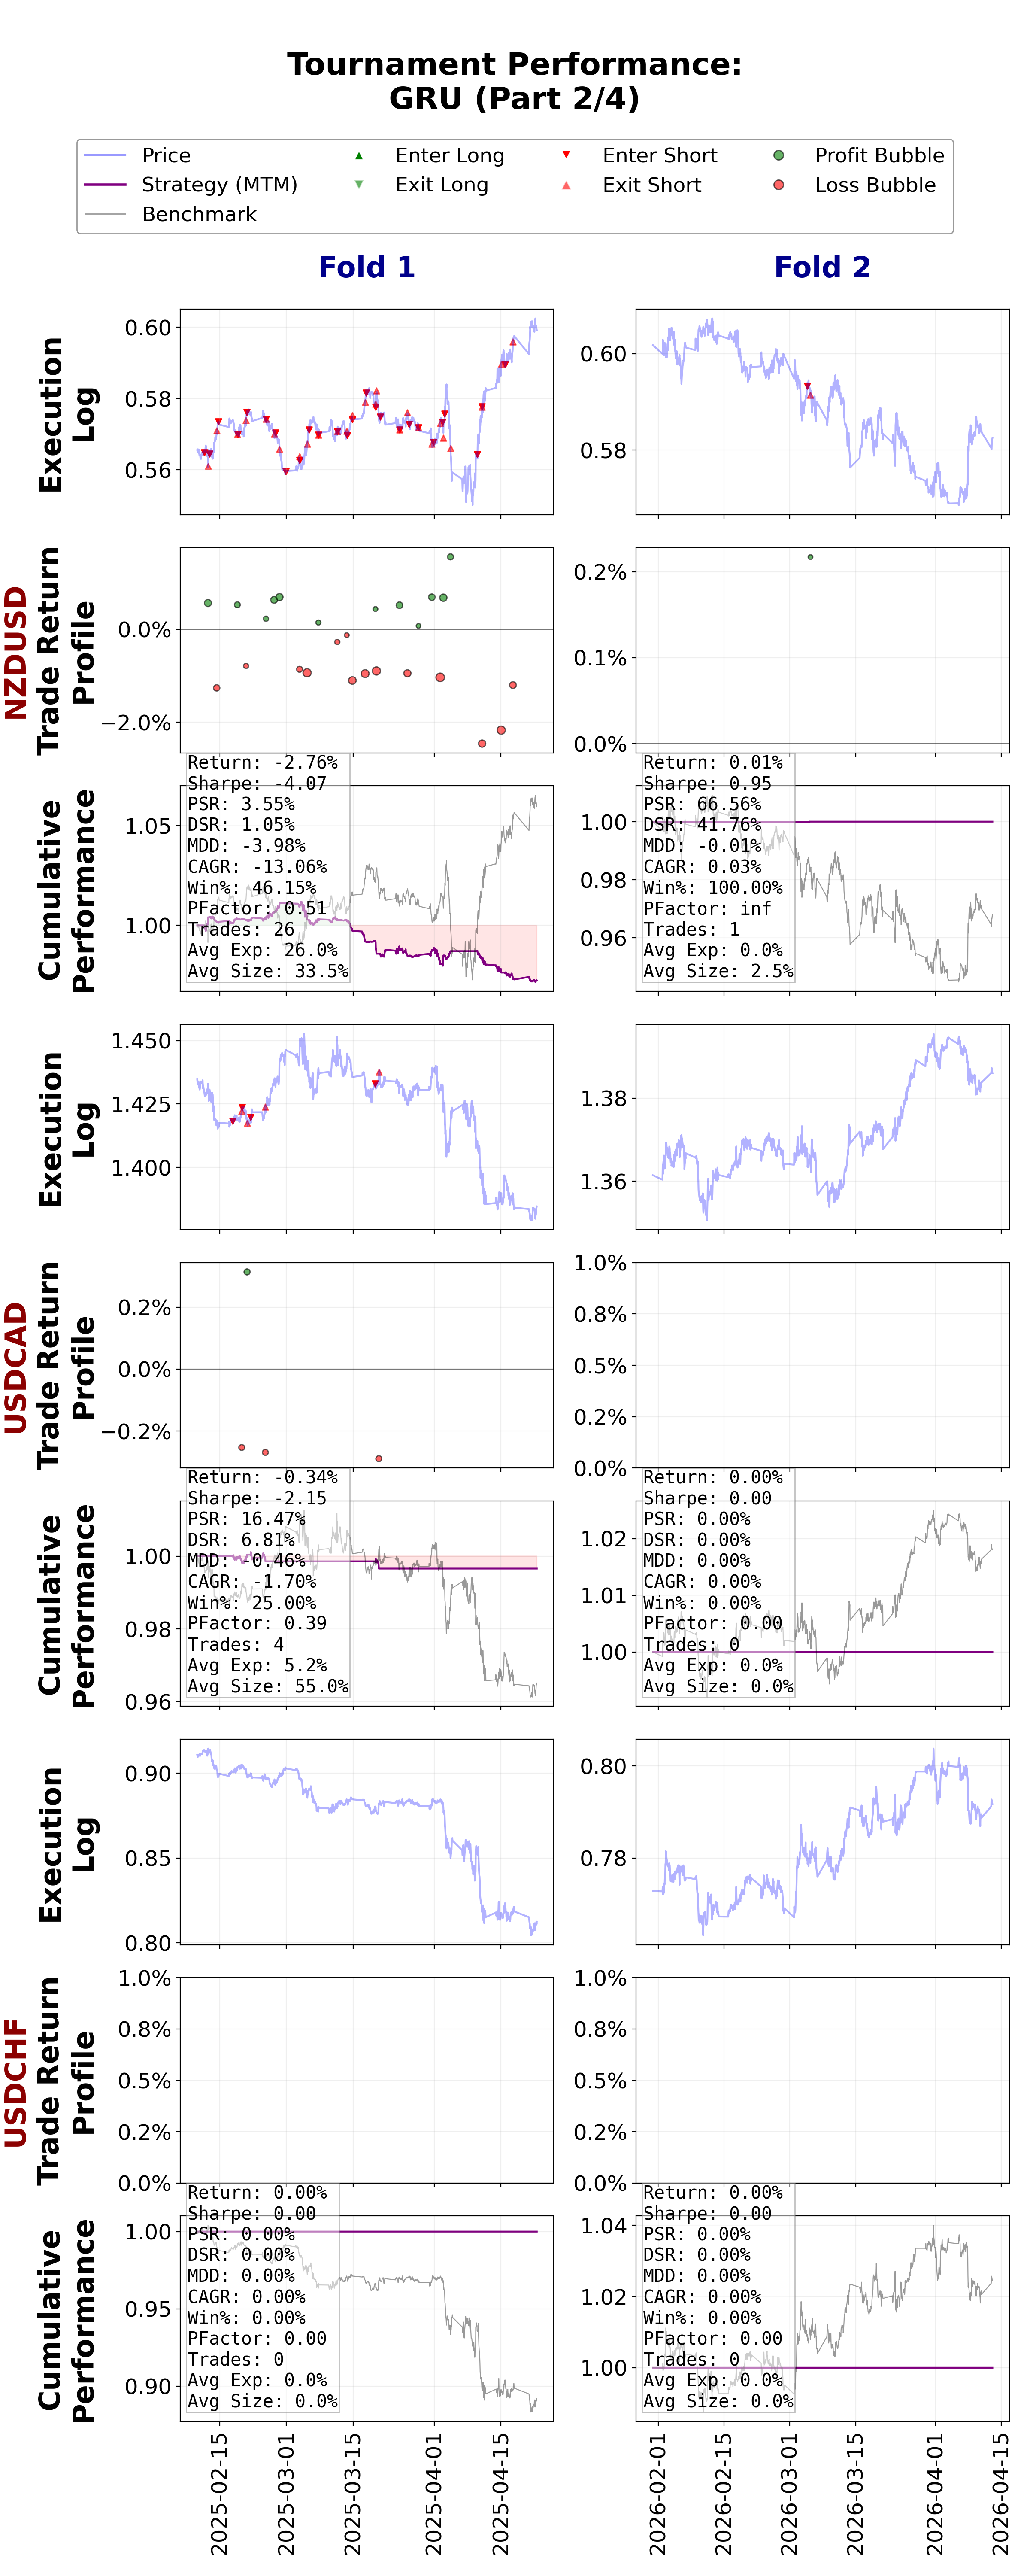
\includegraphics[width=\textwidth]{../data/figures/backtests/tournament_results_GRU_part2.png}
        \caption{Backtest Result of GRU During Tournament (Continued)}
        \label{fig:tournament_results_GRU_2}
    \end{minipage}
\end{figure}

\begin{figure}[H]
    \centering
    \begin{minipage}[t]{0.49\textwidth}
        \centering
        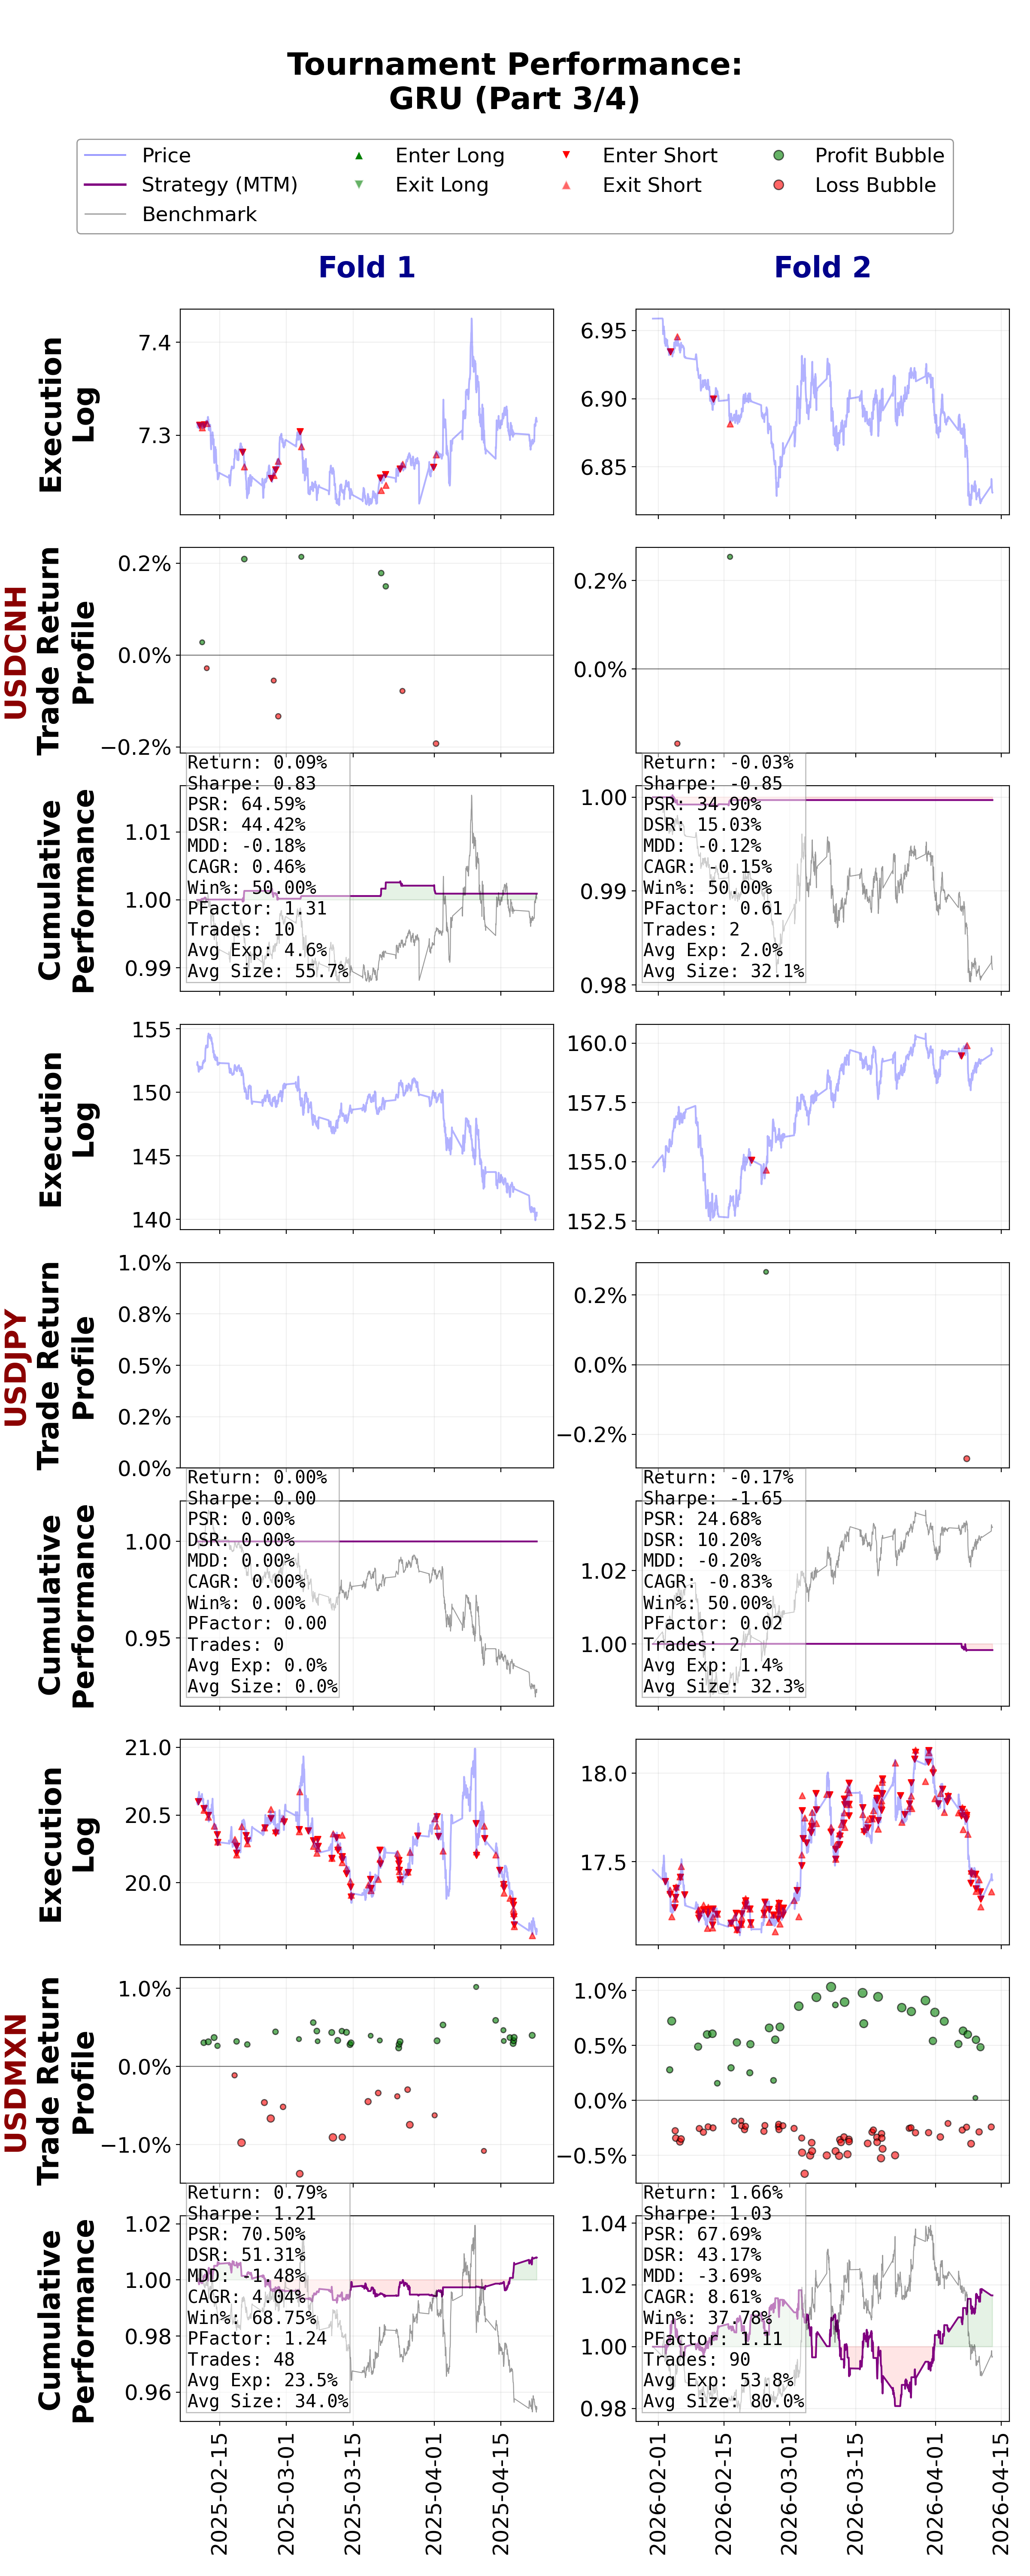
\includegraphics[width=\textwidth]{../data/figures/backtests/tournament_results_GRU_part3.png}
        \caption{Backtest Result of GRU During Tournament (Continued)}
        \label{fig:tournament_results_GRU_3}
    \end{minipage}
    \hfill
    \begin{minipage}[t]{0.49\textwidth}
        \centering
        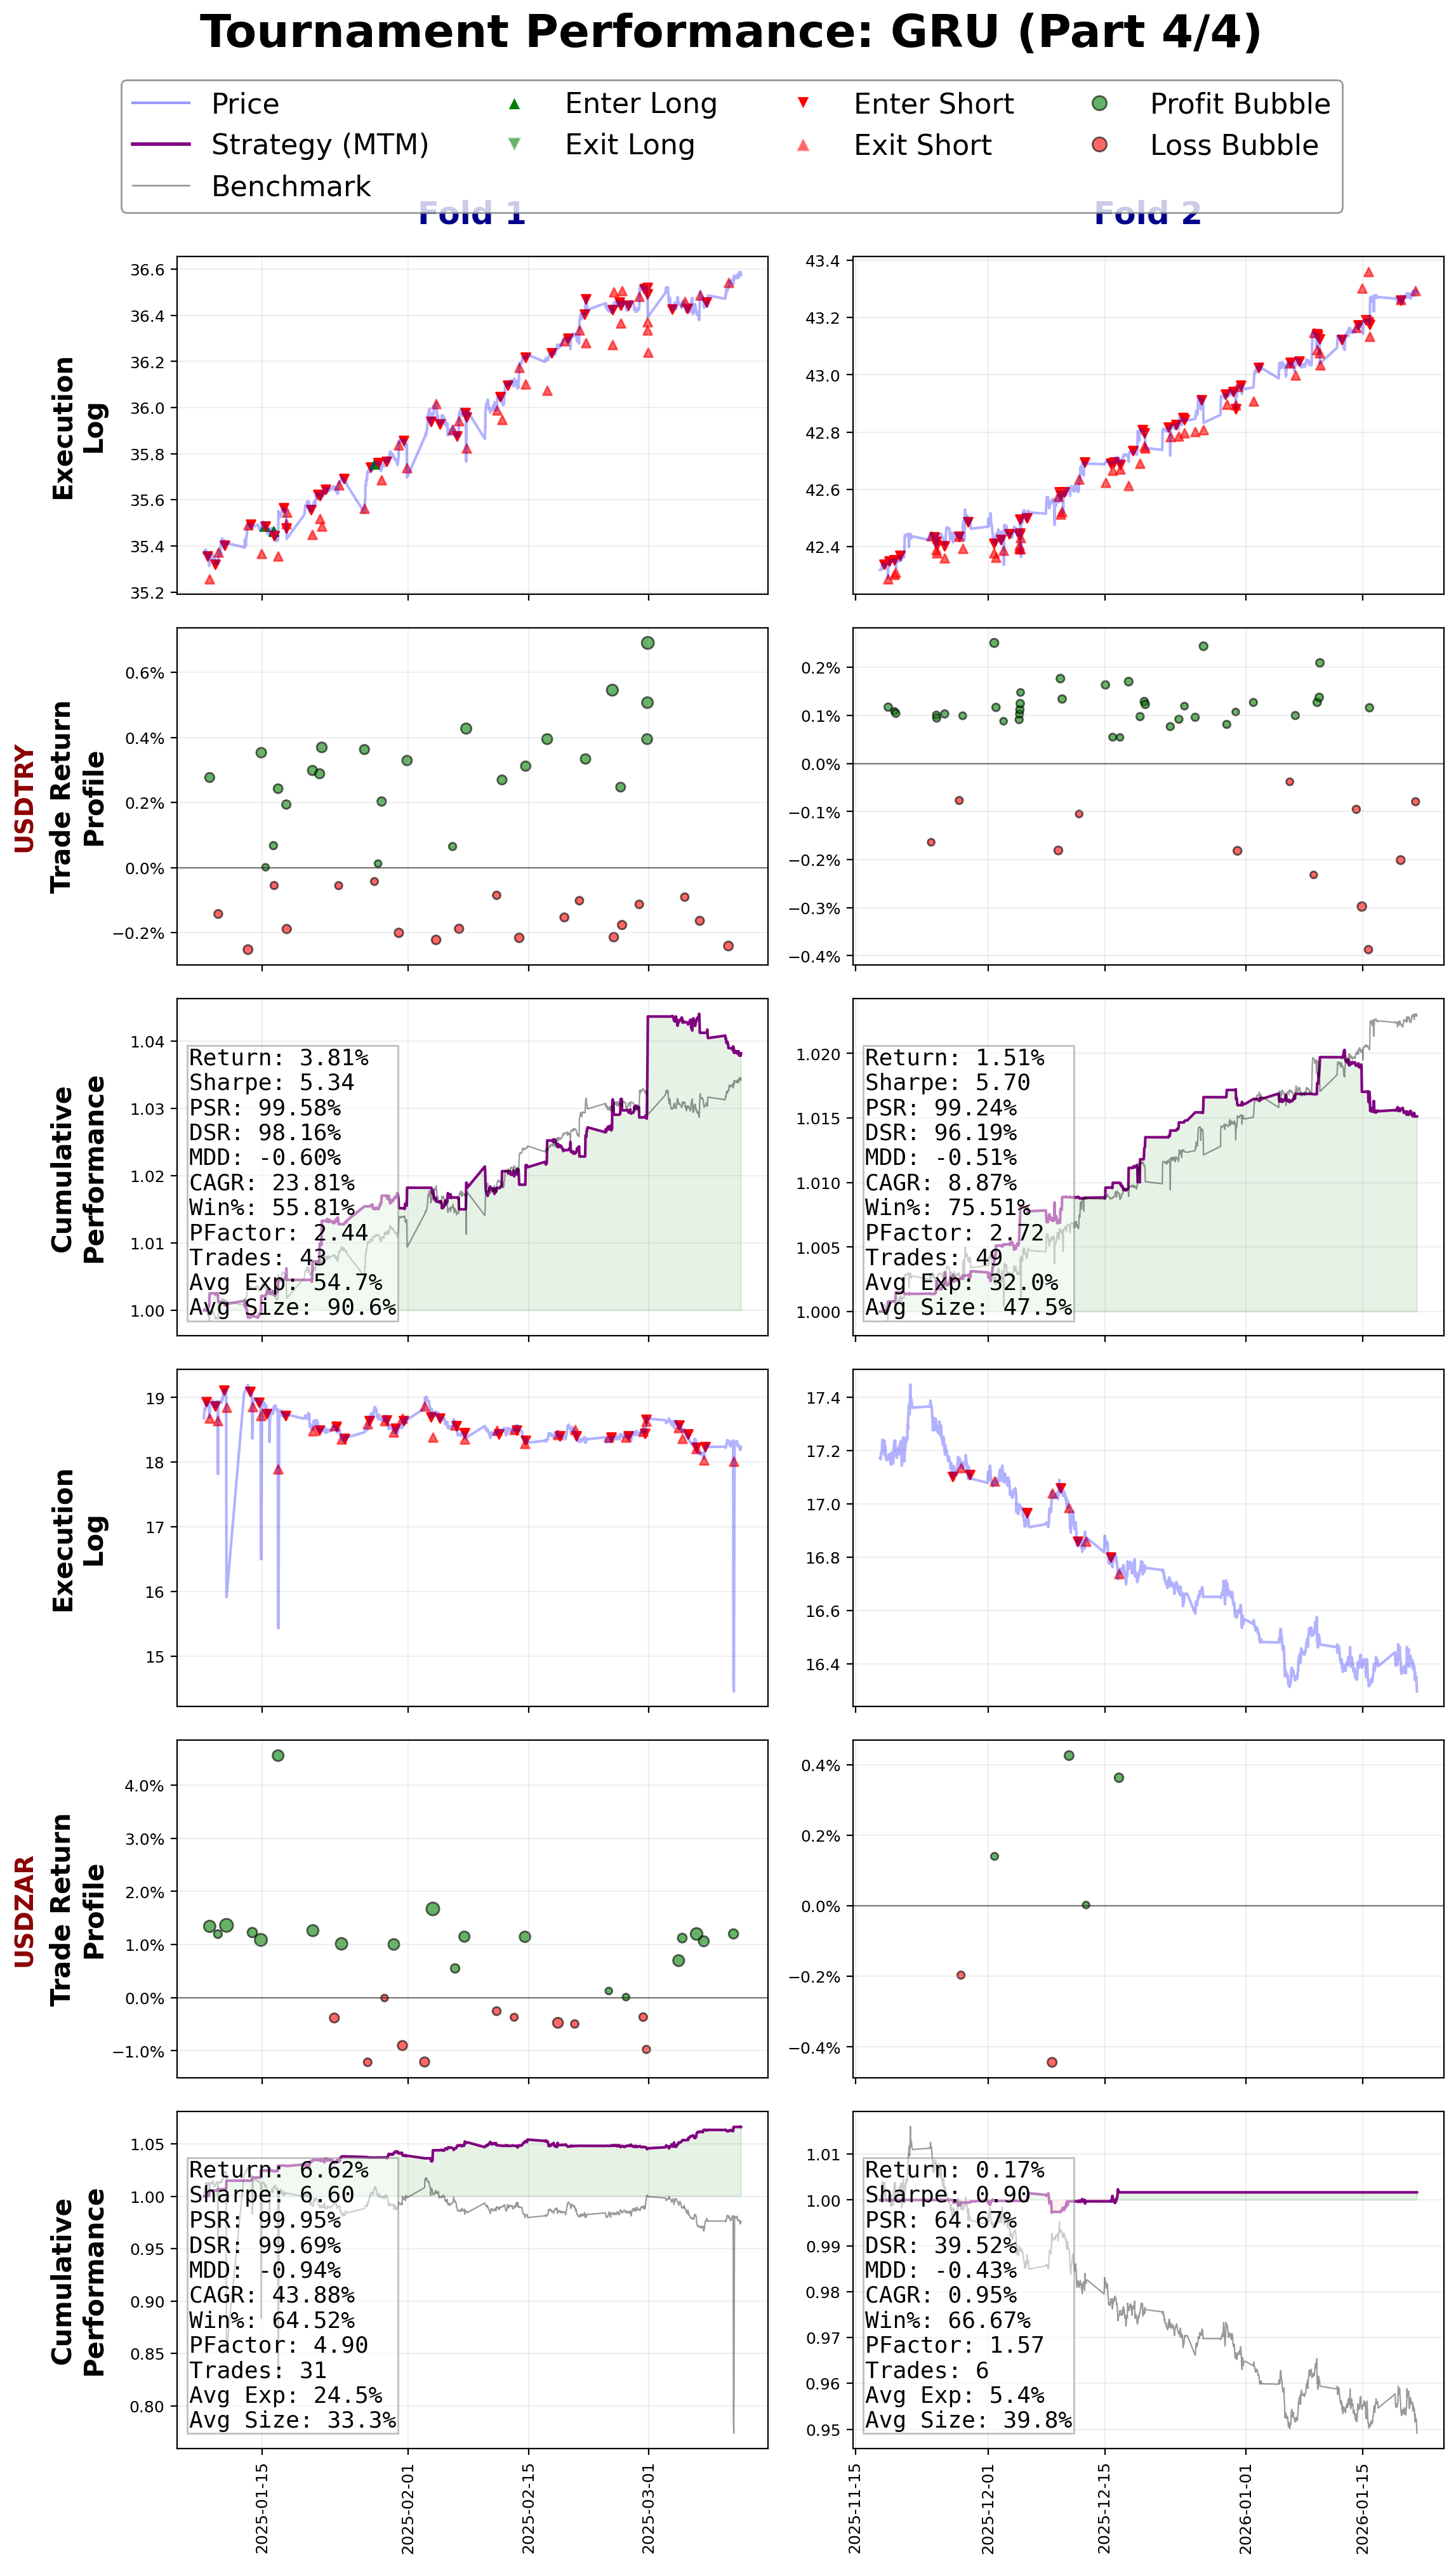
\includegraphics[width=\textwidth]{../data/figures/backtests/tournament_results_GRU_part4.png}
        \caption{Backtest Result of GRU During Tournament (Continued)}
        \label{fig:tournament_results_GRU_4}
    \end{minipage}
\end{figure}


\begin{figure}[H]
    \centering
    \begin{minipage}[t]{0.49\textwidth}
        \centering
        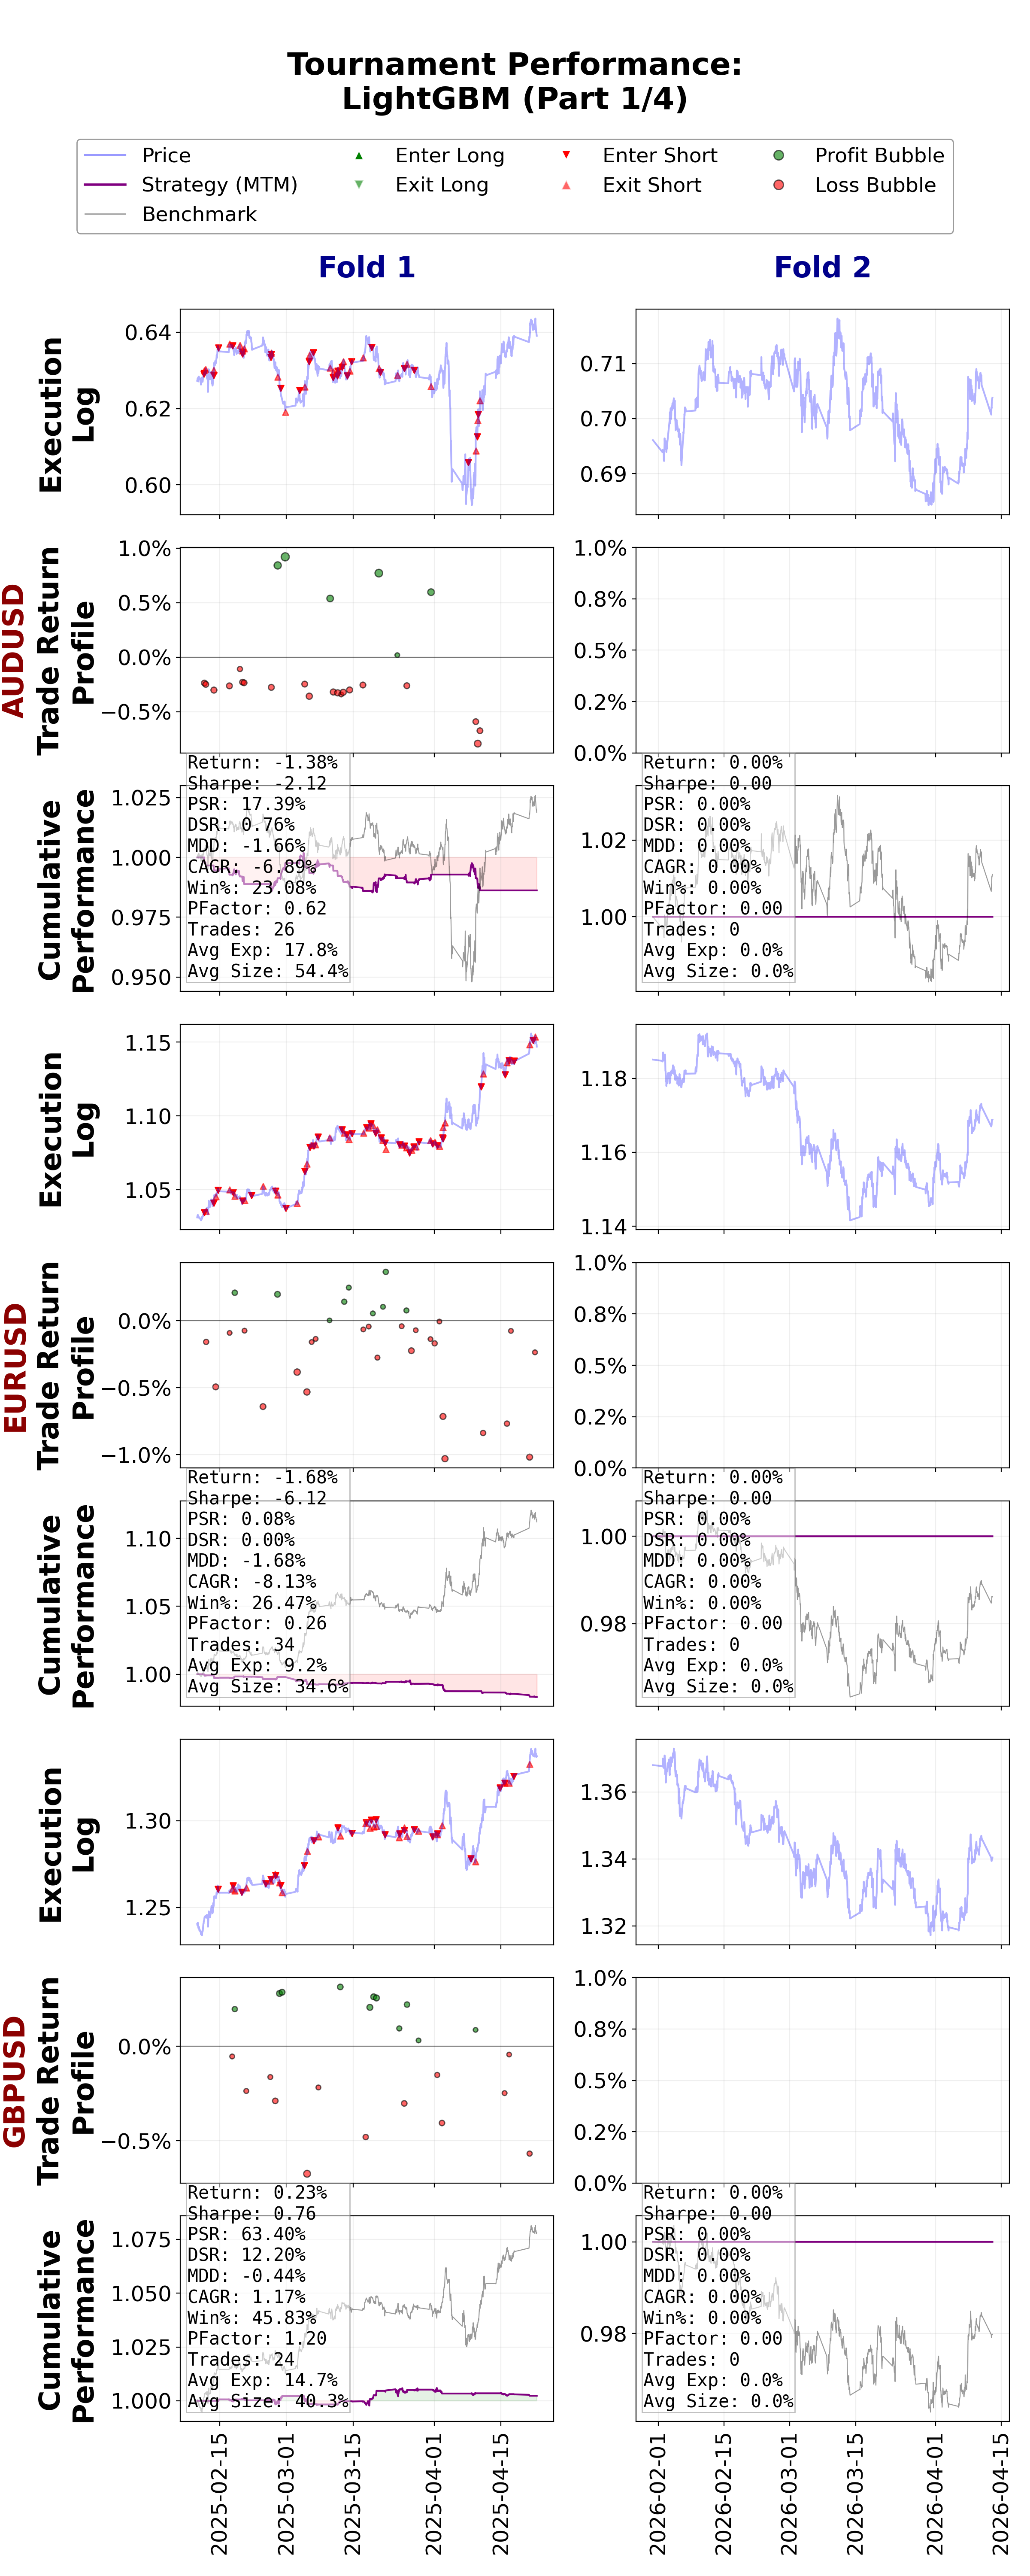
\includegraphics[width=\textwidth]{../data/figures/backtests/tournament_results_LightGBM_part1.png}
        \caption{Backtest Result of LightGBM During Tournament}
        \label{fig:tournament_results_LightGBM_1}
    \end{minipage}
    \hfill
    \begin{minipage}[t]{0.49\textwidth}
        \centering
        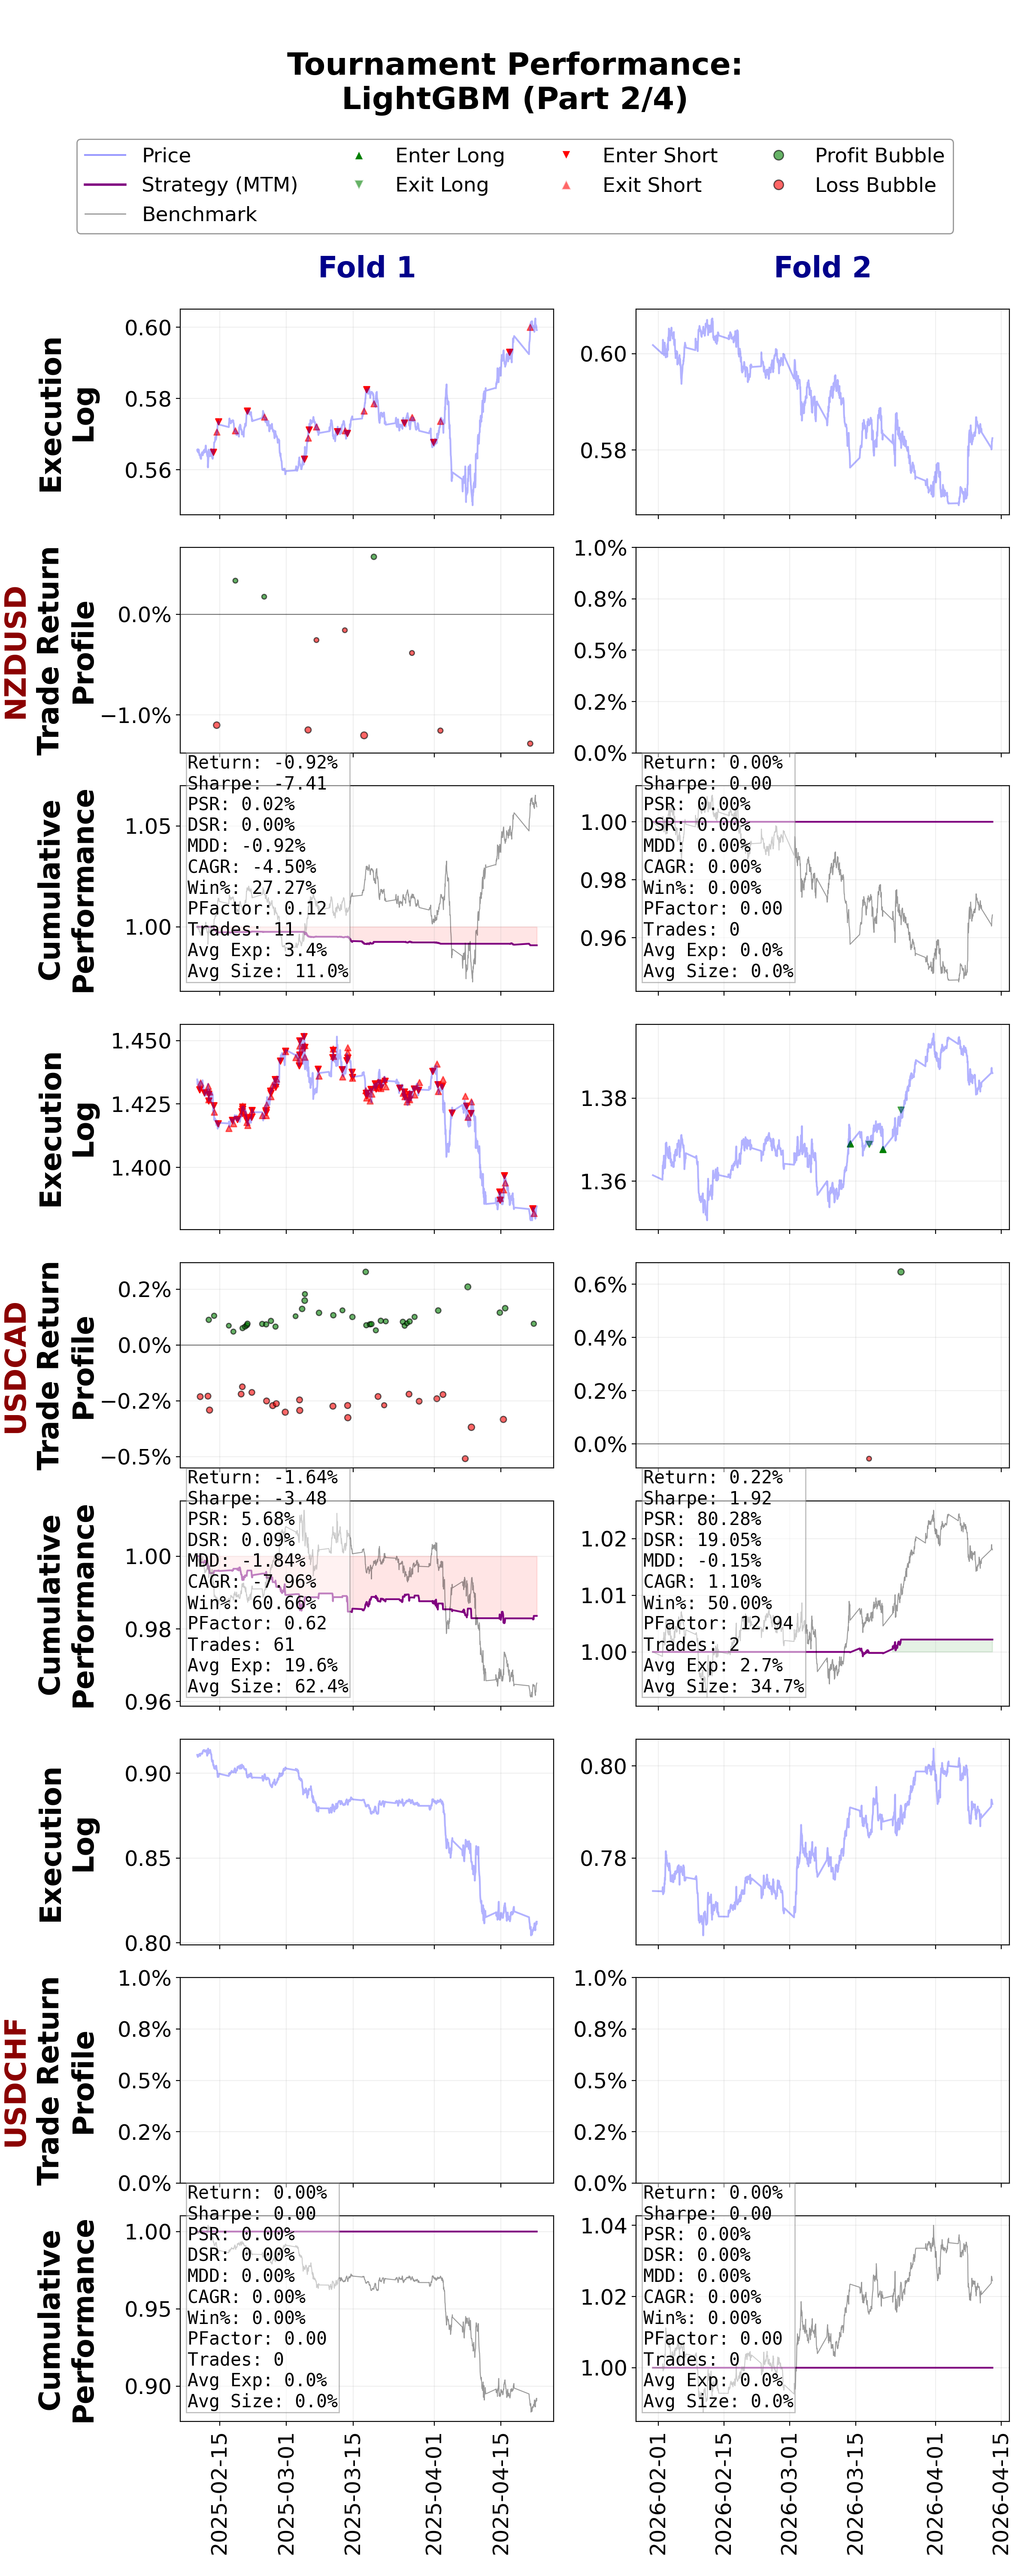
\includegraphics[width=\textwidth]{../data/figures/backtests/tournament_results_LightGBM_part2.png}
        \caption{Backtest Result of LightGBM During Tournament (Continued)}
        \label{fig:tournament_results_LightGBM_2}
    \end{minipage}
\end{figure}

\begin{figure}[H]
    \centering
    \begin{minipage}[t]{0.49\textwidth}
        \centering
        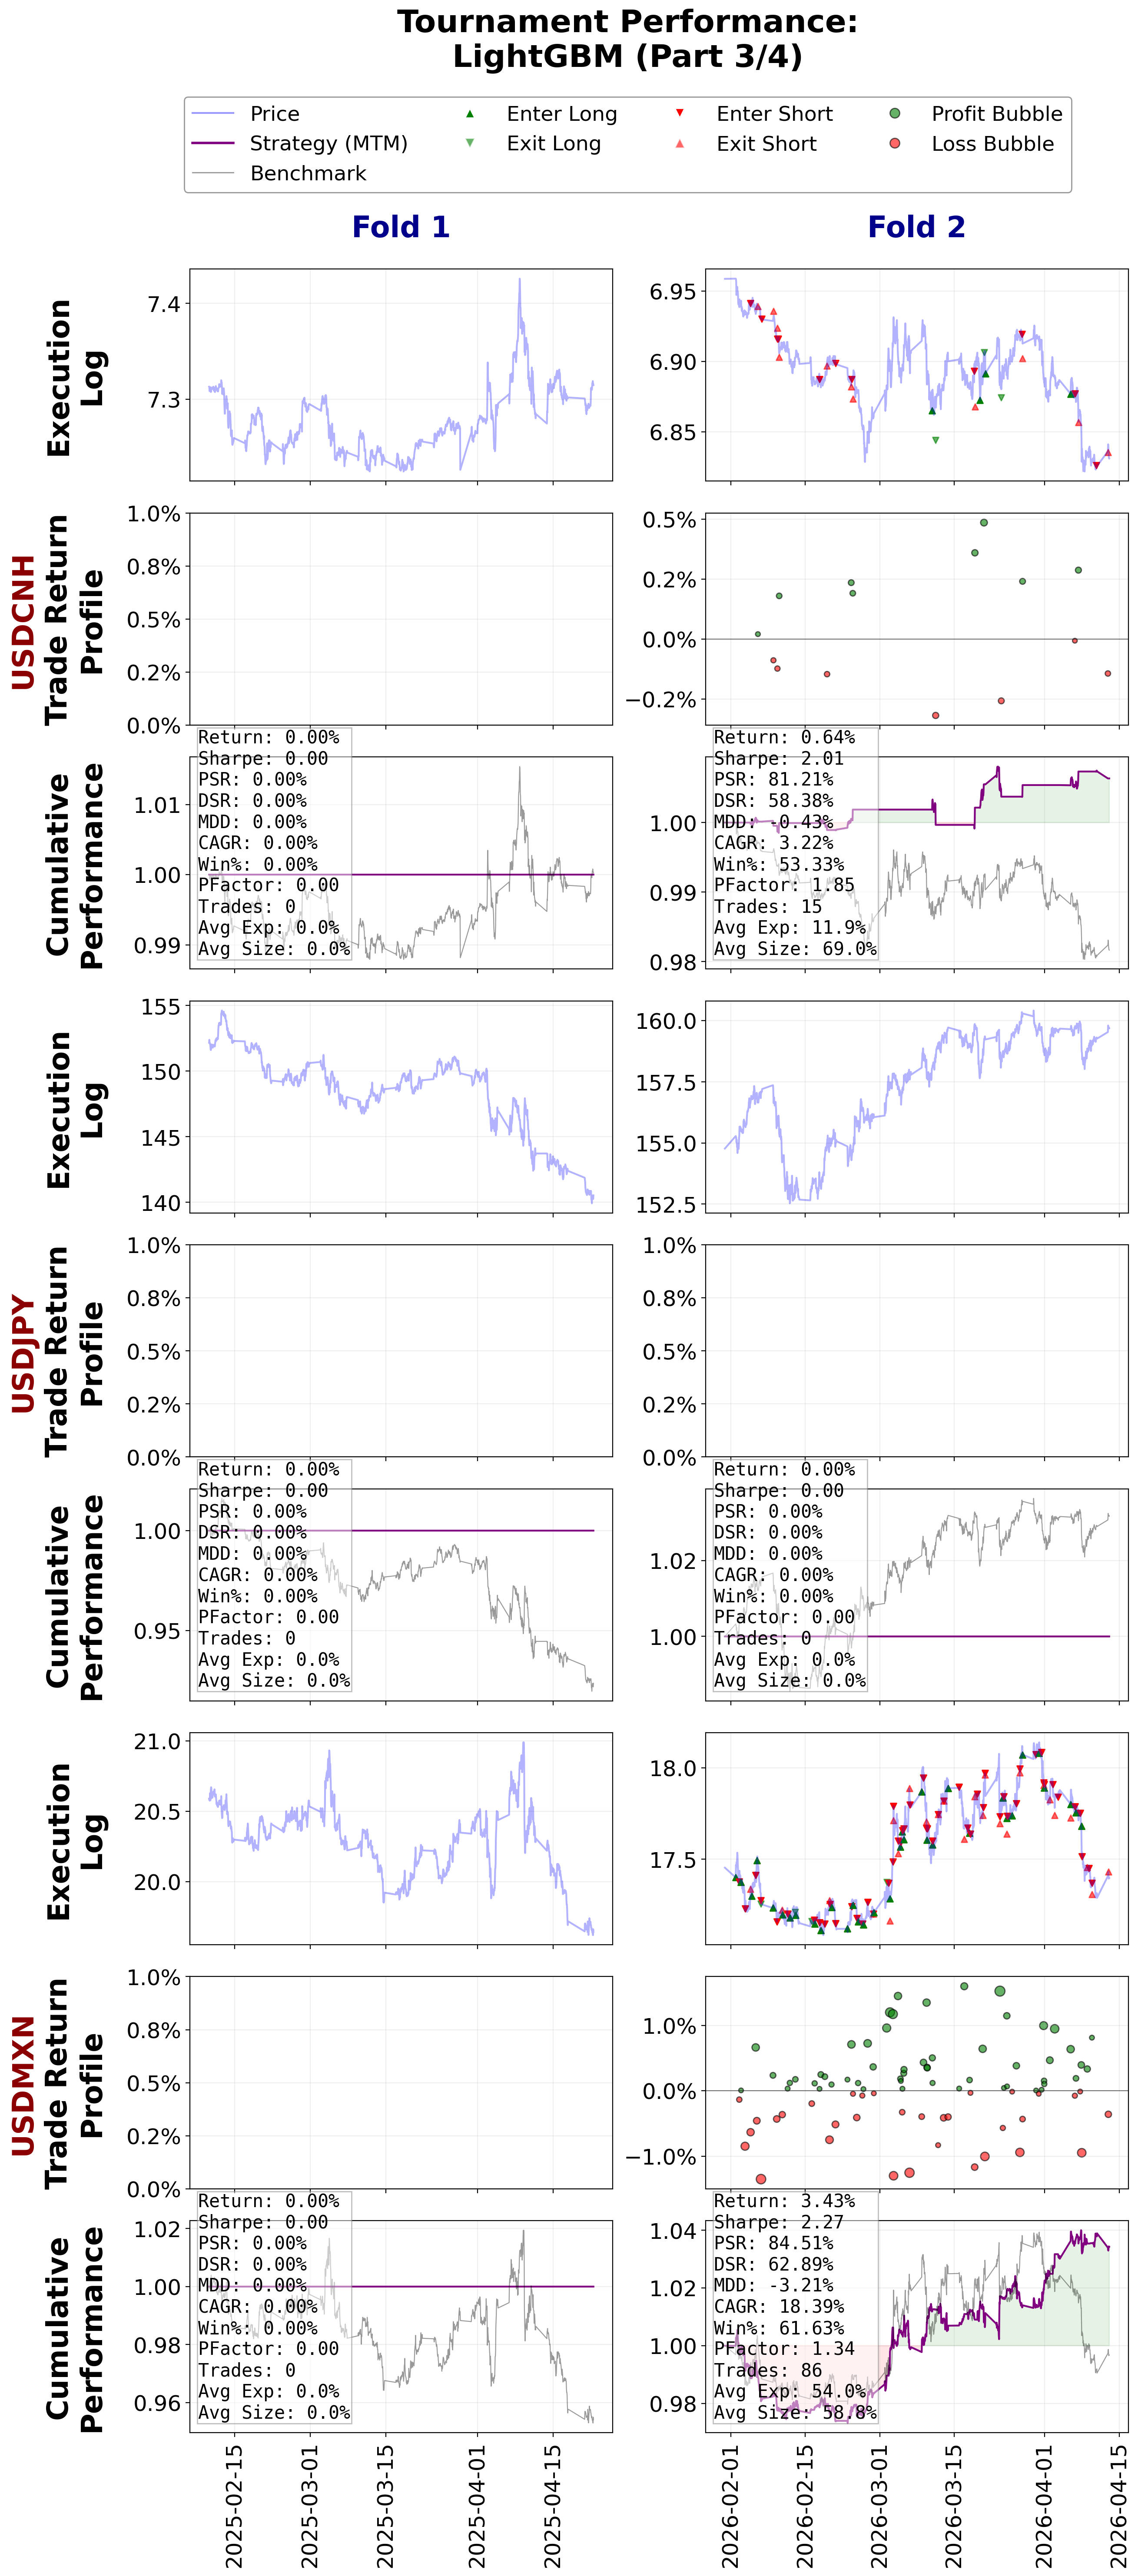
\includegraphics[width=\textwidth]{../data/figures/backtests/tournament_results_LightGBM_part3.png}
        \caption{Backtest Result of LightGBM During Tournament (Continued)}
        \label{fig:tournament_results_LightGBM_3}
    \end{minipage}
    \hfill
    \begin{minipage}[t]{0.49\textwidth}
        \centering
        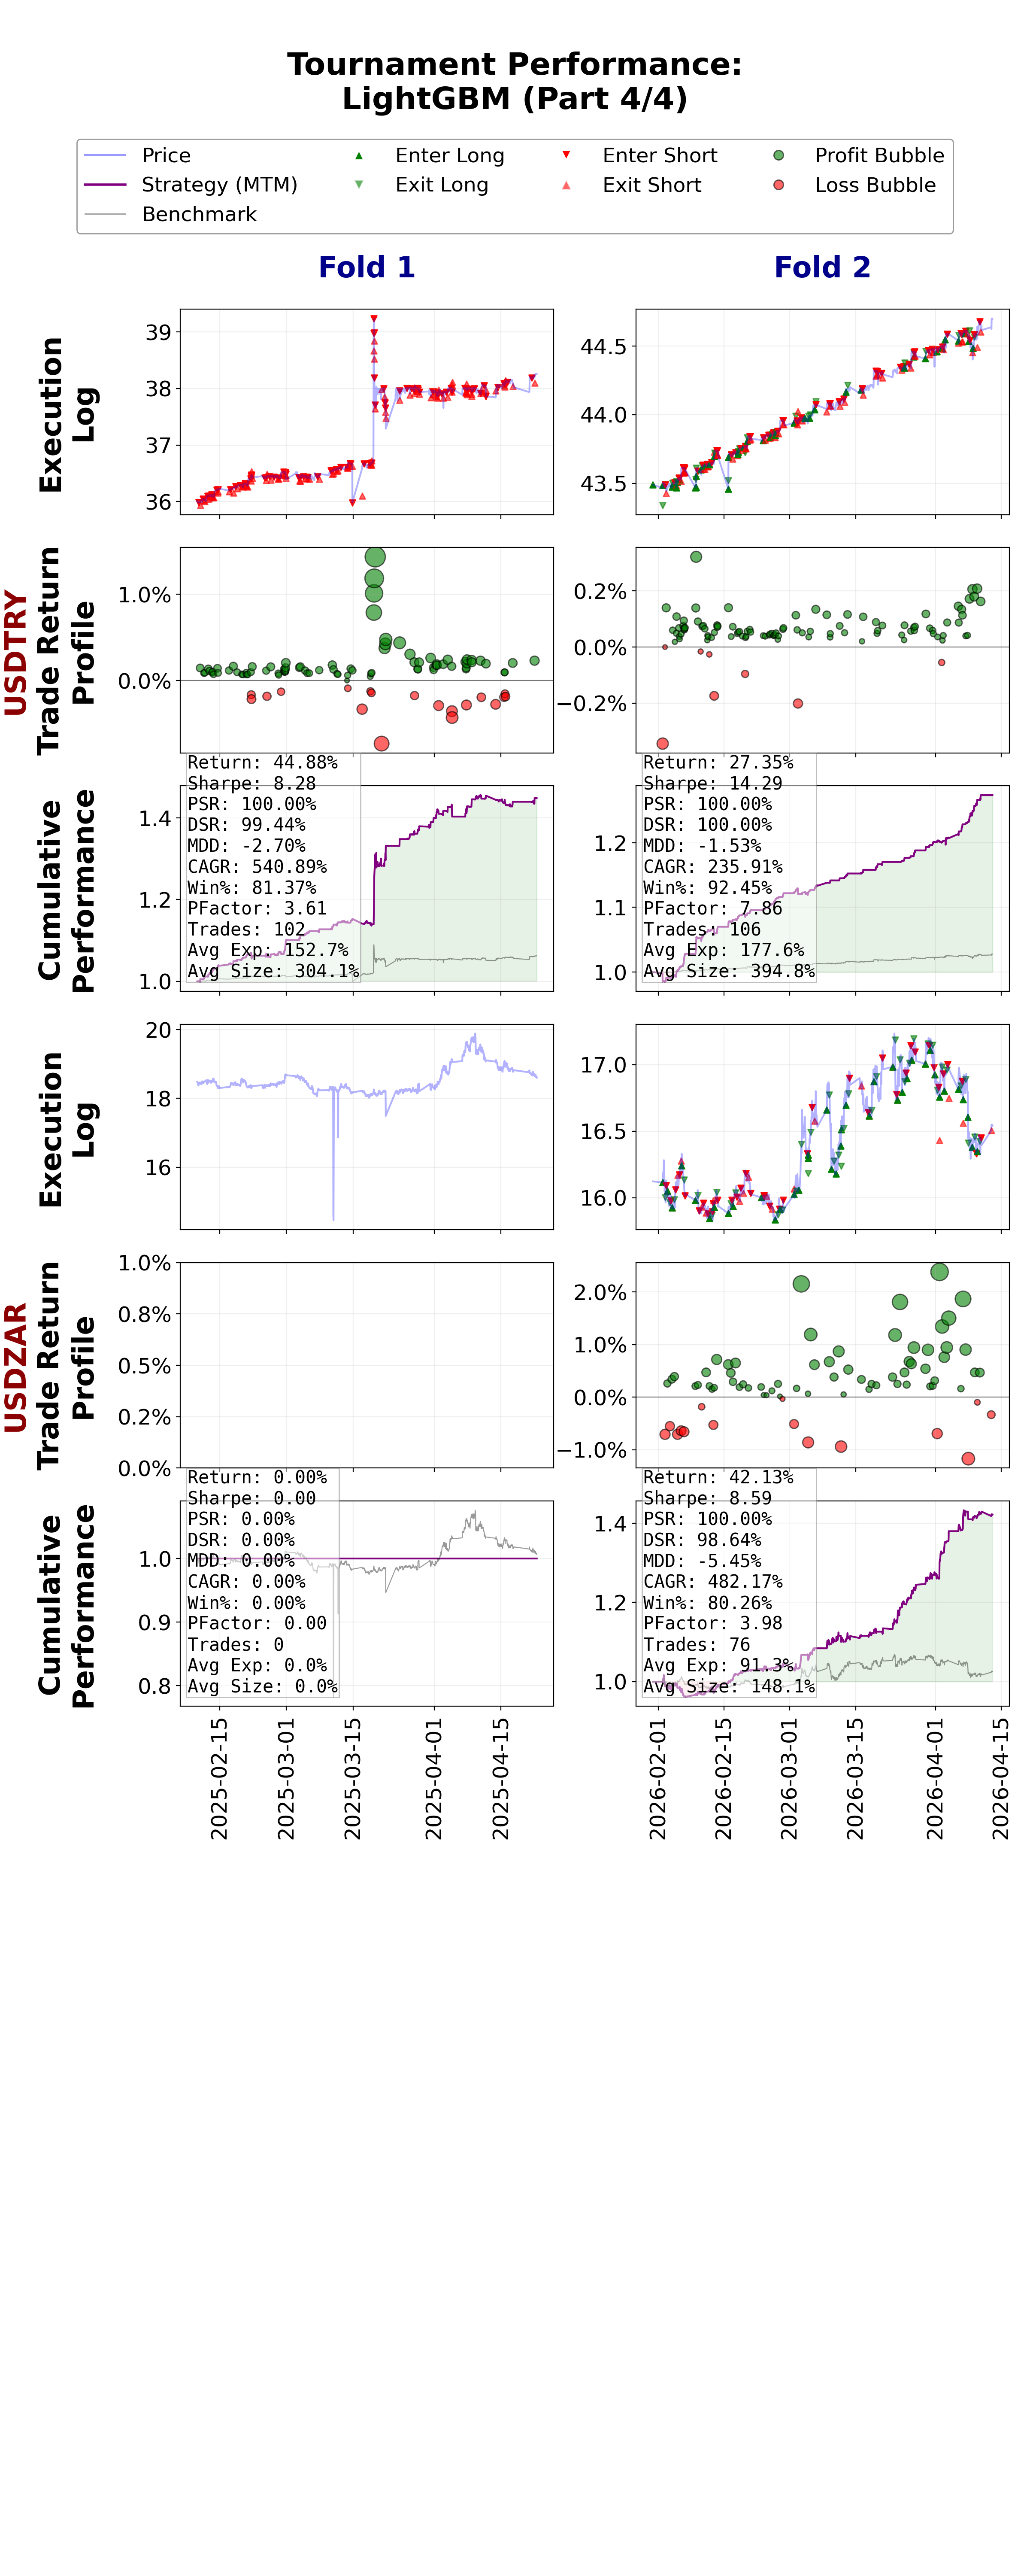
\includegraphics[width=\textwidth]{../data/figures/backtests/tournament_results_LightGBM_part4.png}
        \caption{Backtest Result of LightGBM During Tournament (Continued)}
        \label{fig:tournament_results_LightGBM_4}
    \end{minipage}
\end{figure}


\begin{figure}[H]
    \centering
    \begin{minipage}[t]{0.49\textwidth}
        \centering
        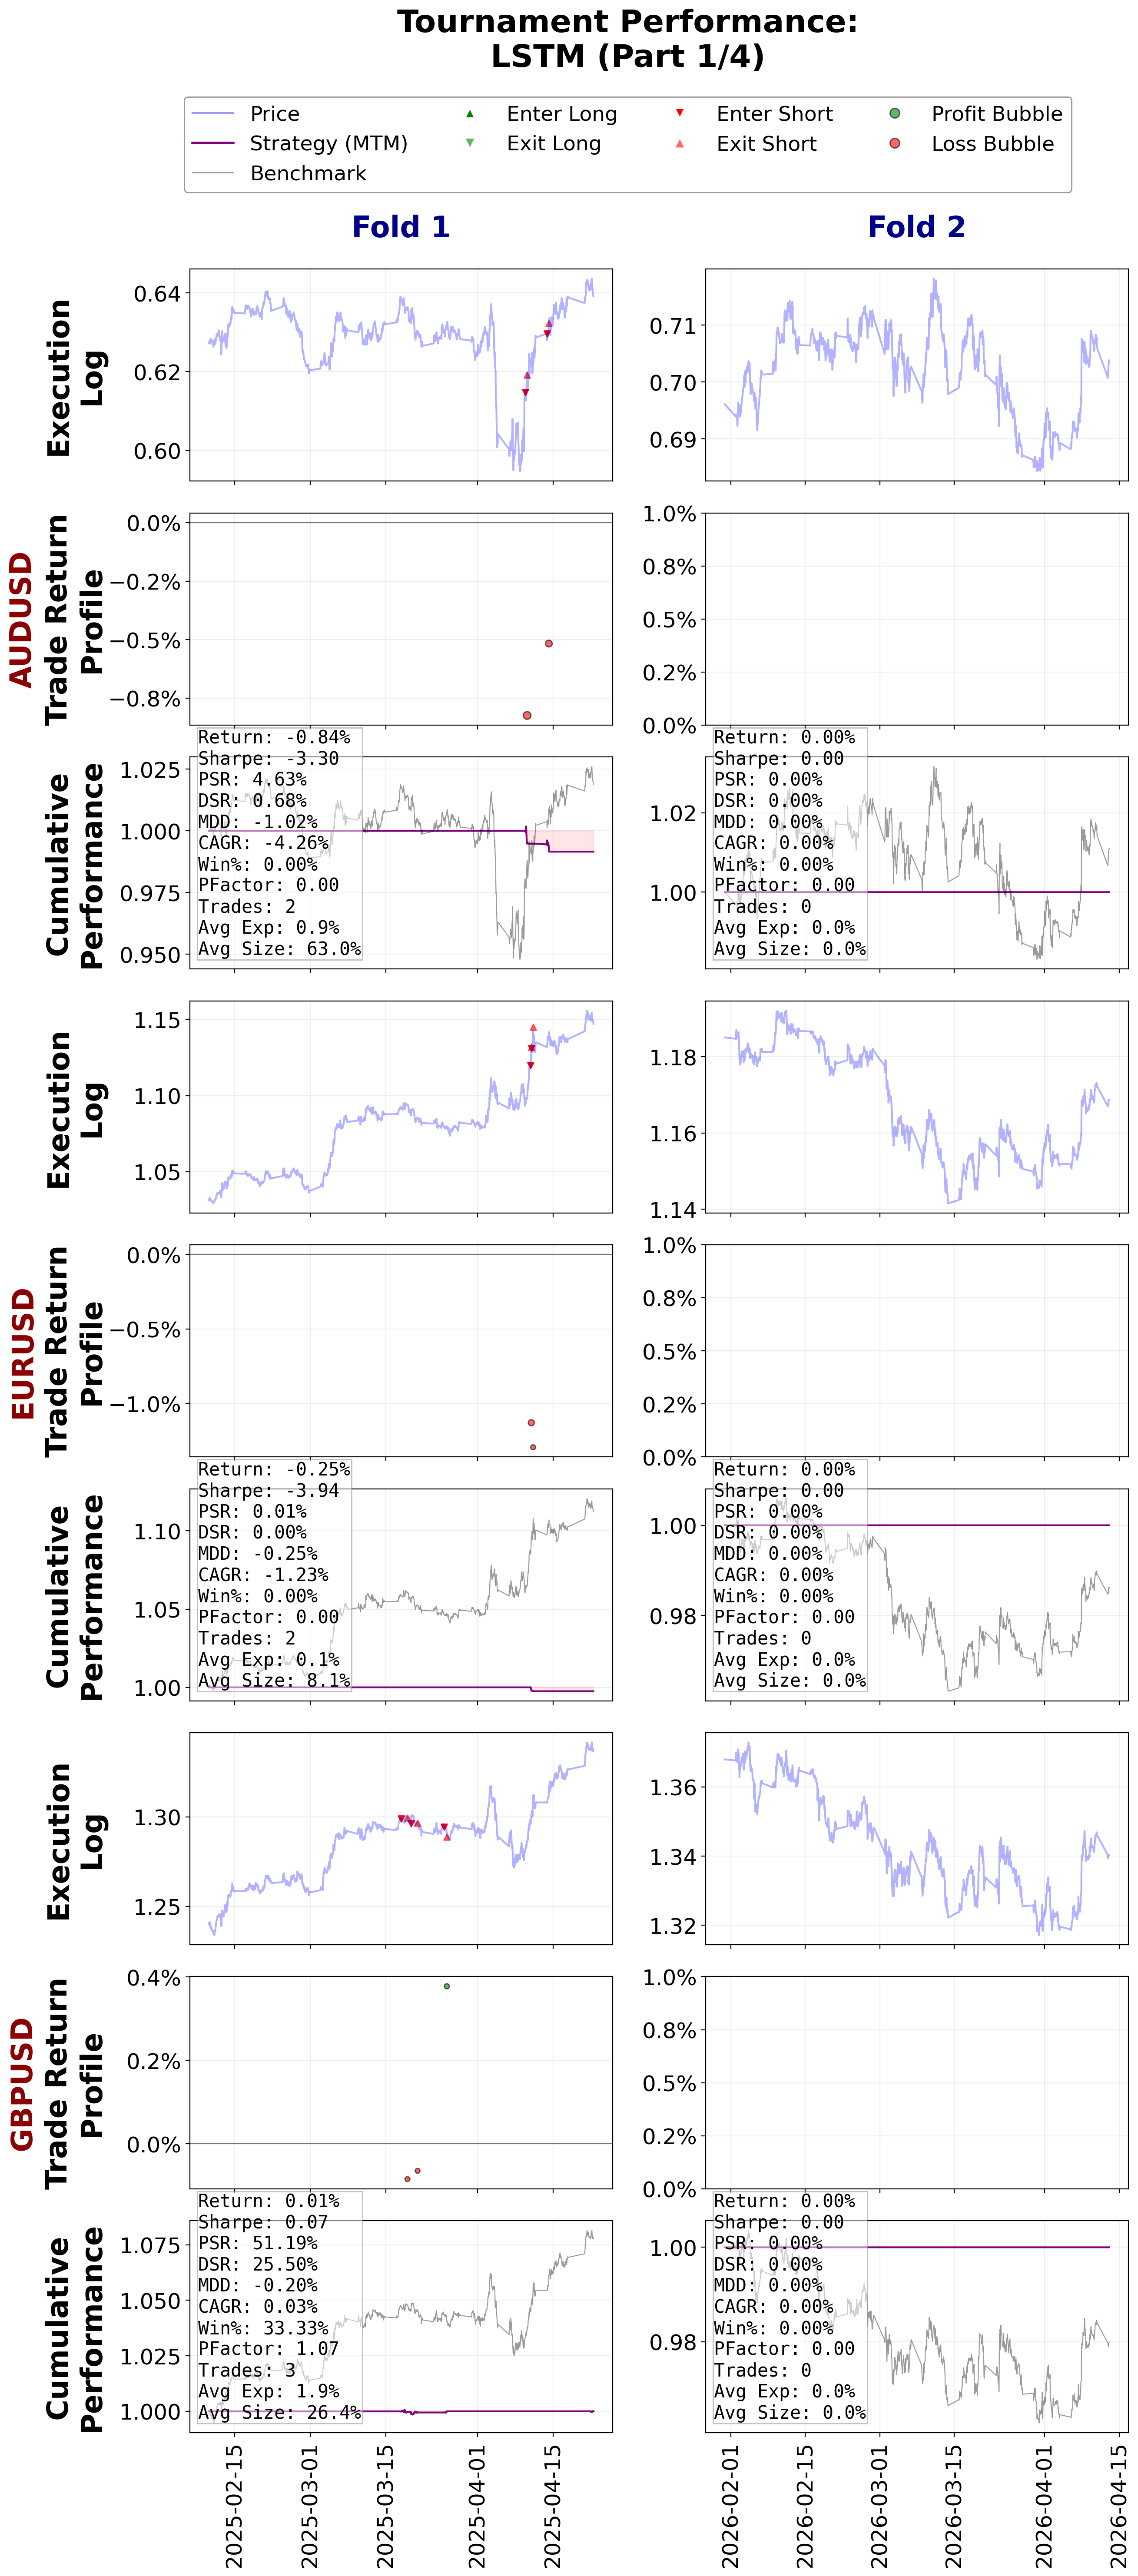
\includegraphics[width=\textwidth]{../data/figures/backtests/tournament_results_LSTM_part1.png}
        \caption{Backtest Result of LSTM During Tournament}
        \label{fig:tournament_results_LSTM_1}
    \end{minipage}
    \hfill
    \begin{minipage}[t]{0.49\textwidth}
        \centering
        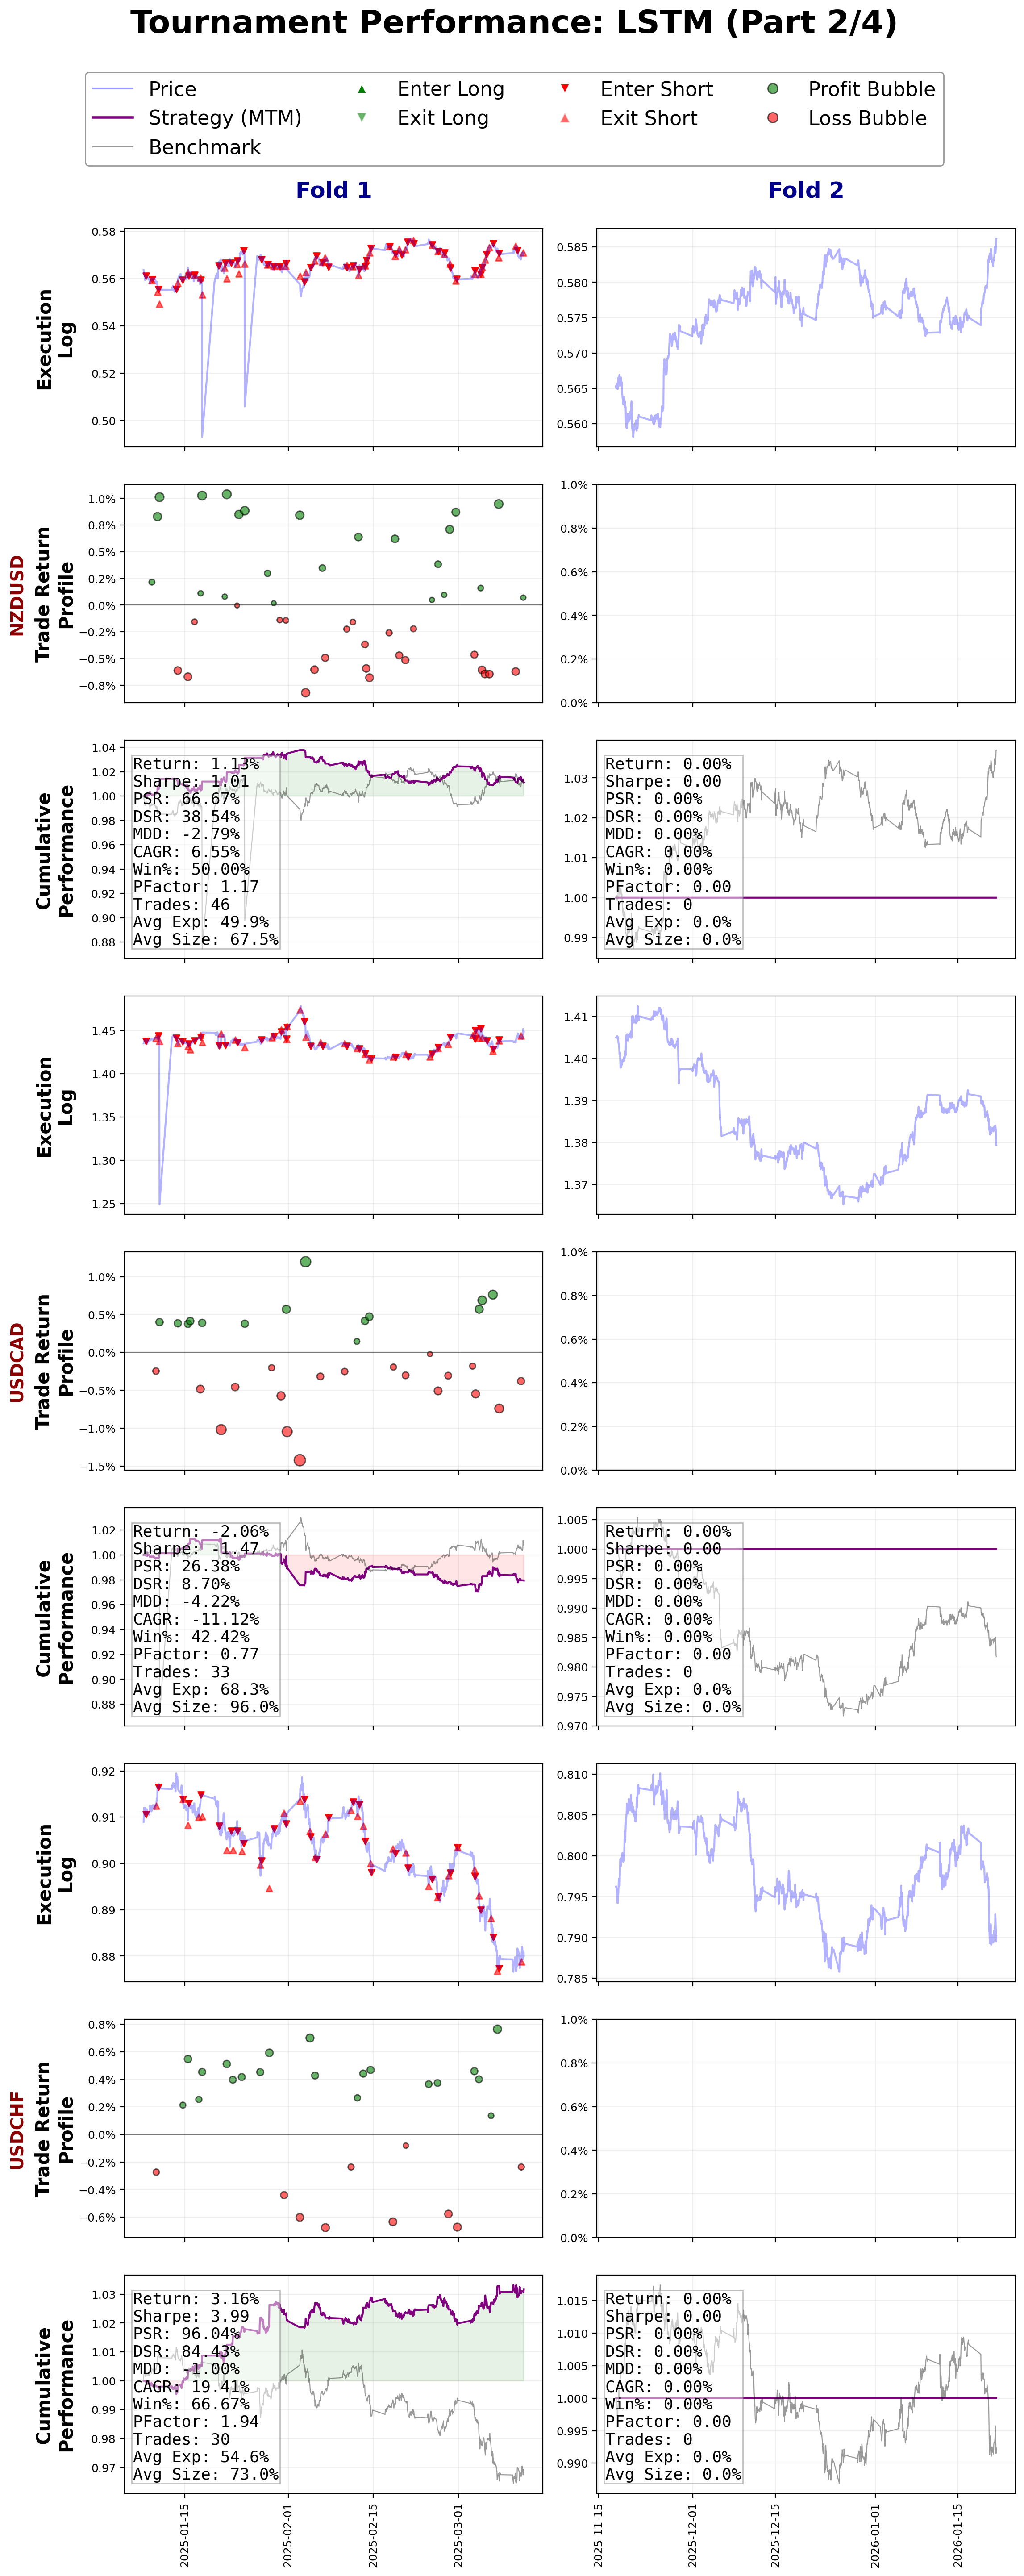
\includegraphics[width=\textwidth]{../data/figures/backtests/tournament_results_LSTM_part2.png}
        \caption{Backtest Result of LSTM During Tournament (Continued)}
        \label{fig:tournament_results_LSTM_2}
    \end{minipage}
\end{figure}

\begin{figure}[H]
    \centering
    \begin{minipage}[t]{0.49\textwidth}
        \centering
        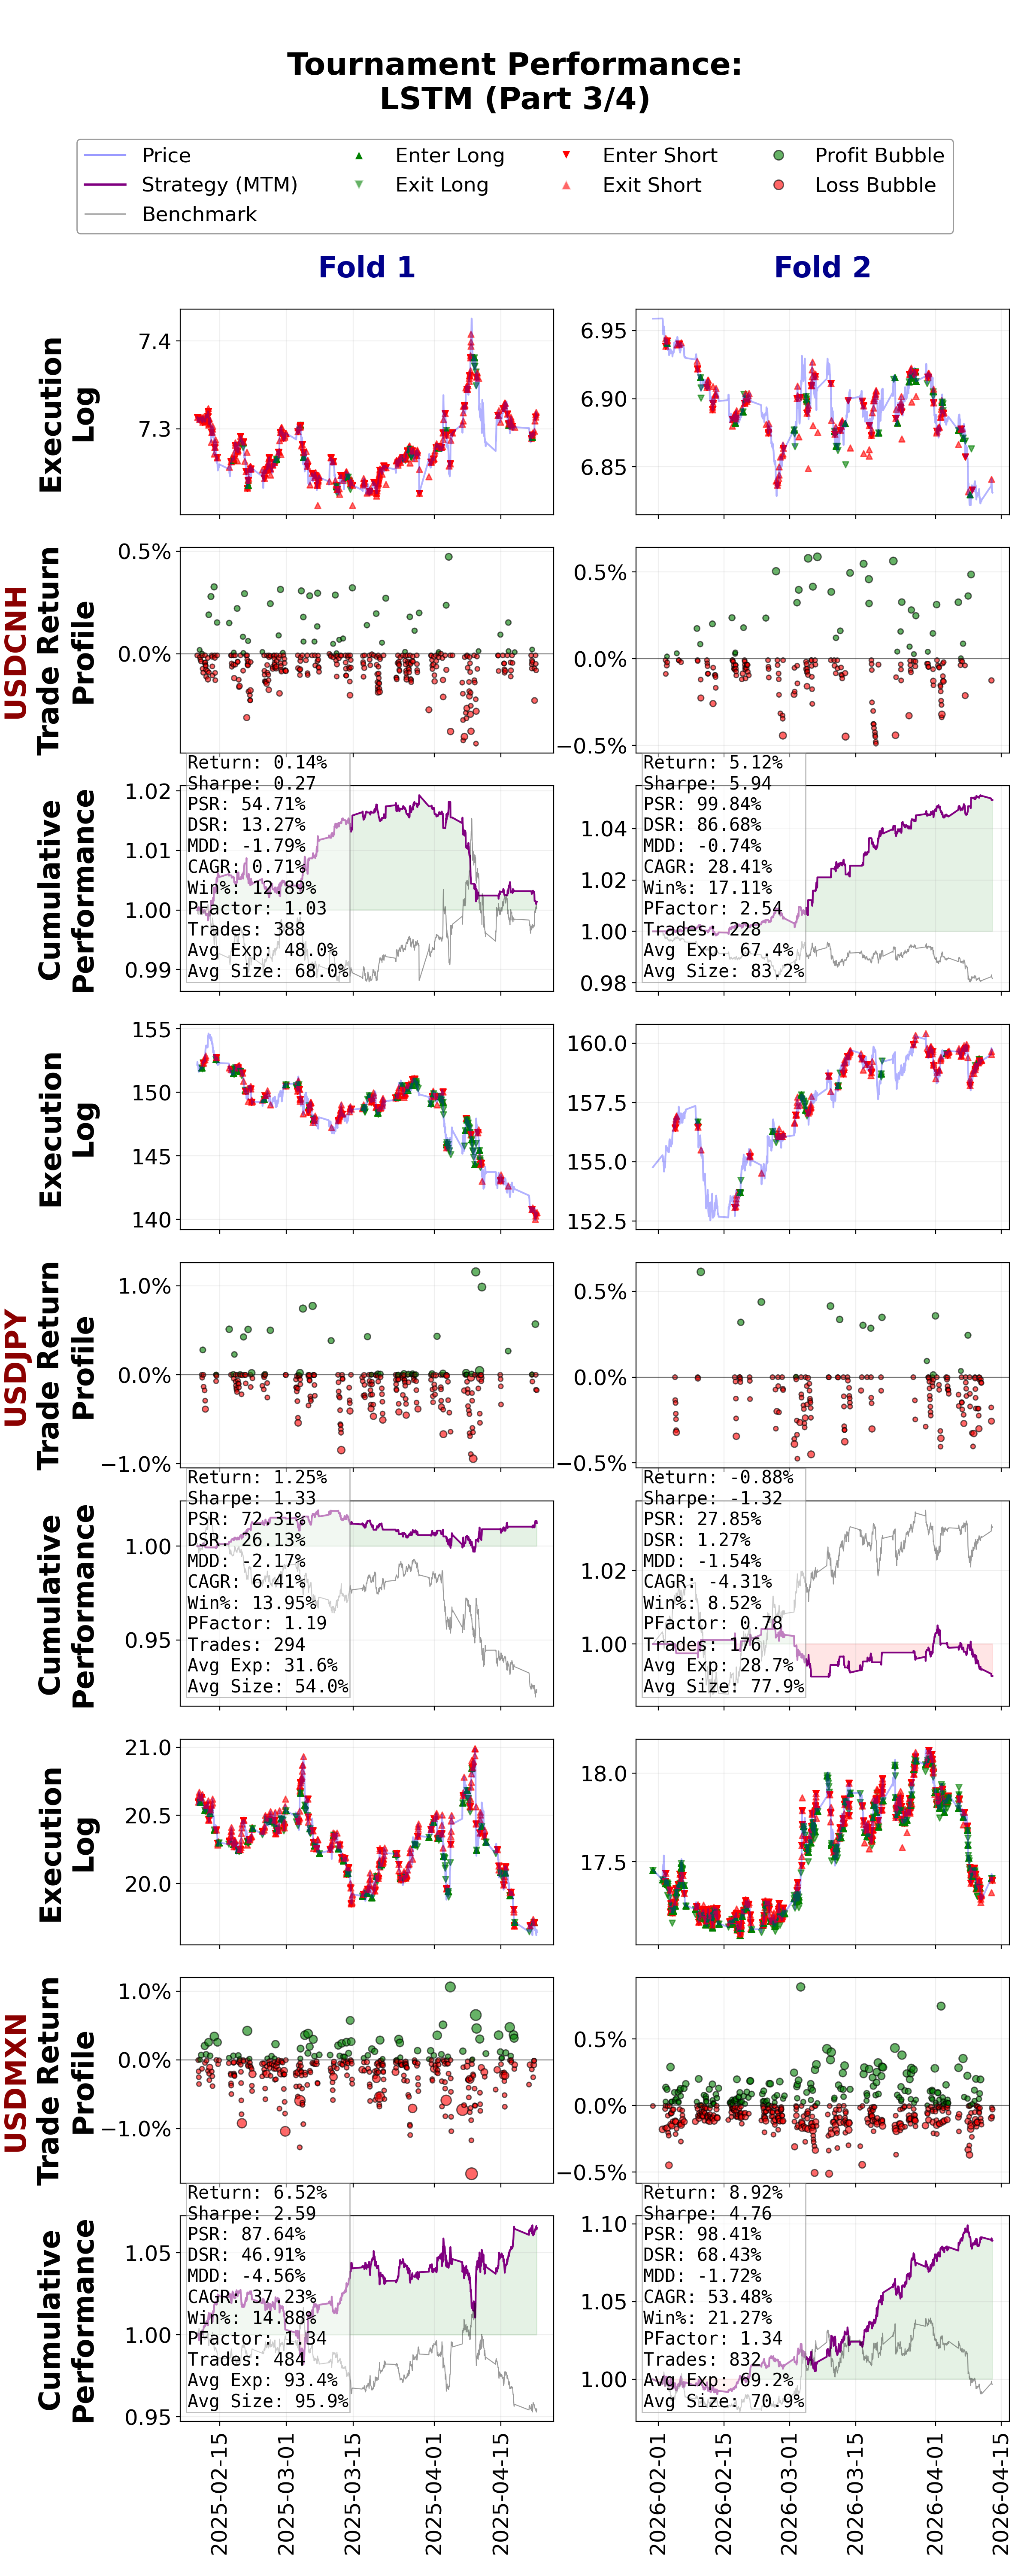
\includegraphics[width=\textwidth]{../data/figures/backtests/tournament_results_LSTM_part3.png}
        \caption{Backtest Result of LSTM During Tournament (Continued)}
        \label{fig:tournament_results_LSTM_3}
    \end{minipage}
    \hfill
    \begin{minipage}[t]{0.49\textwidth}
        \centering
        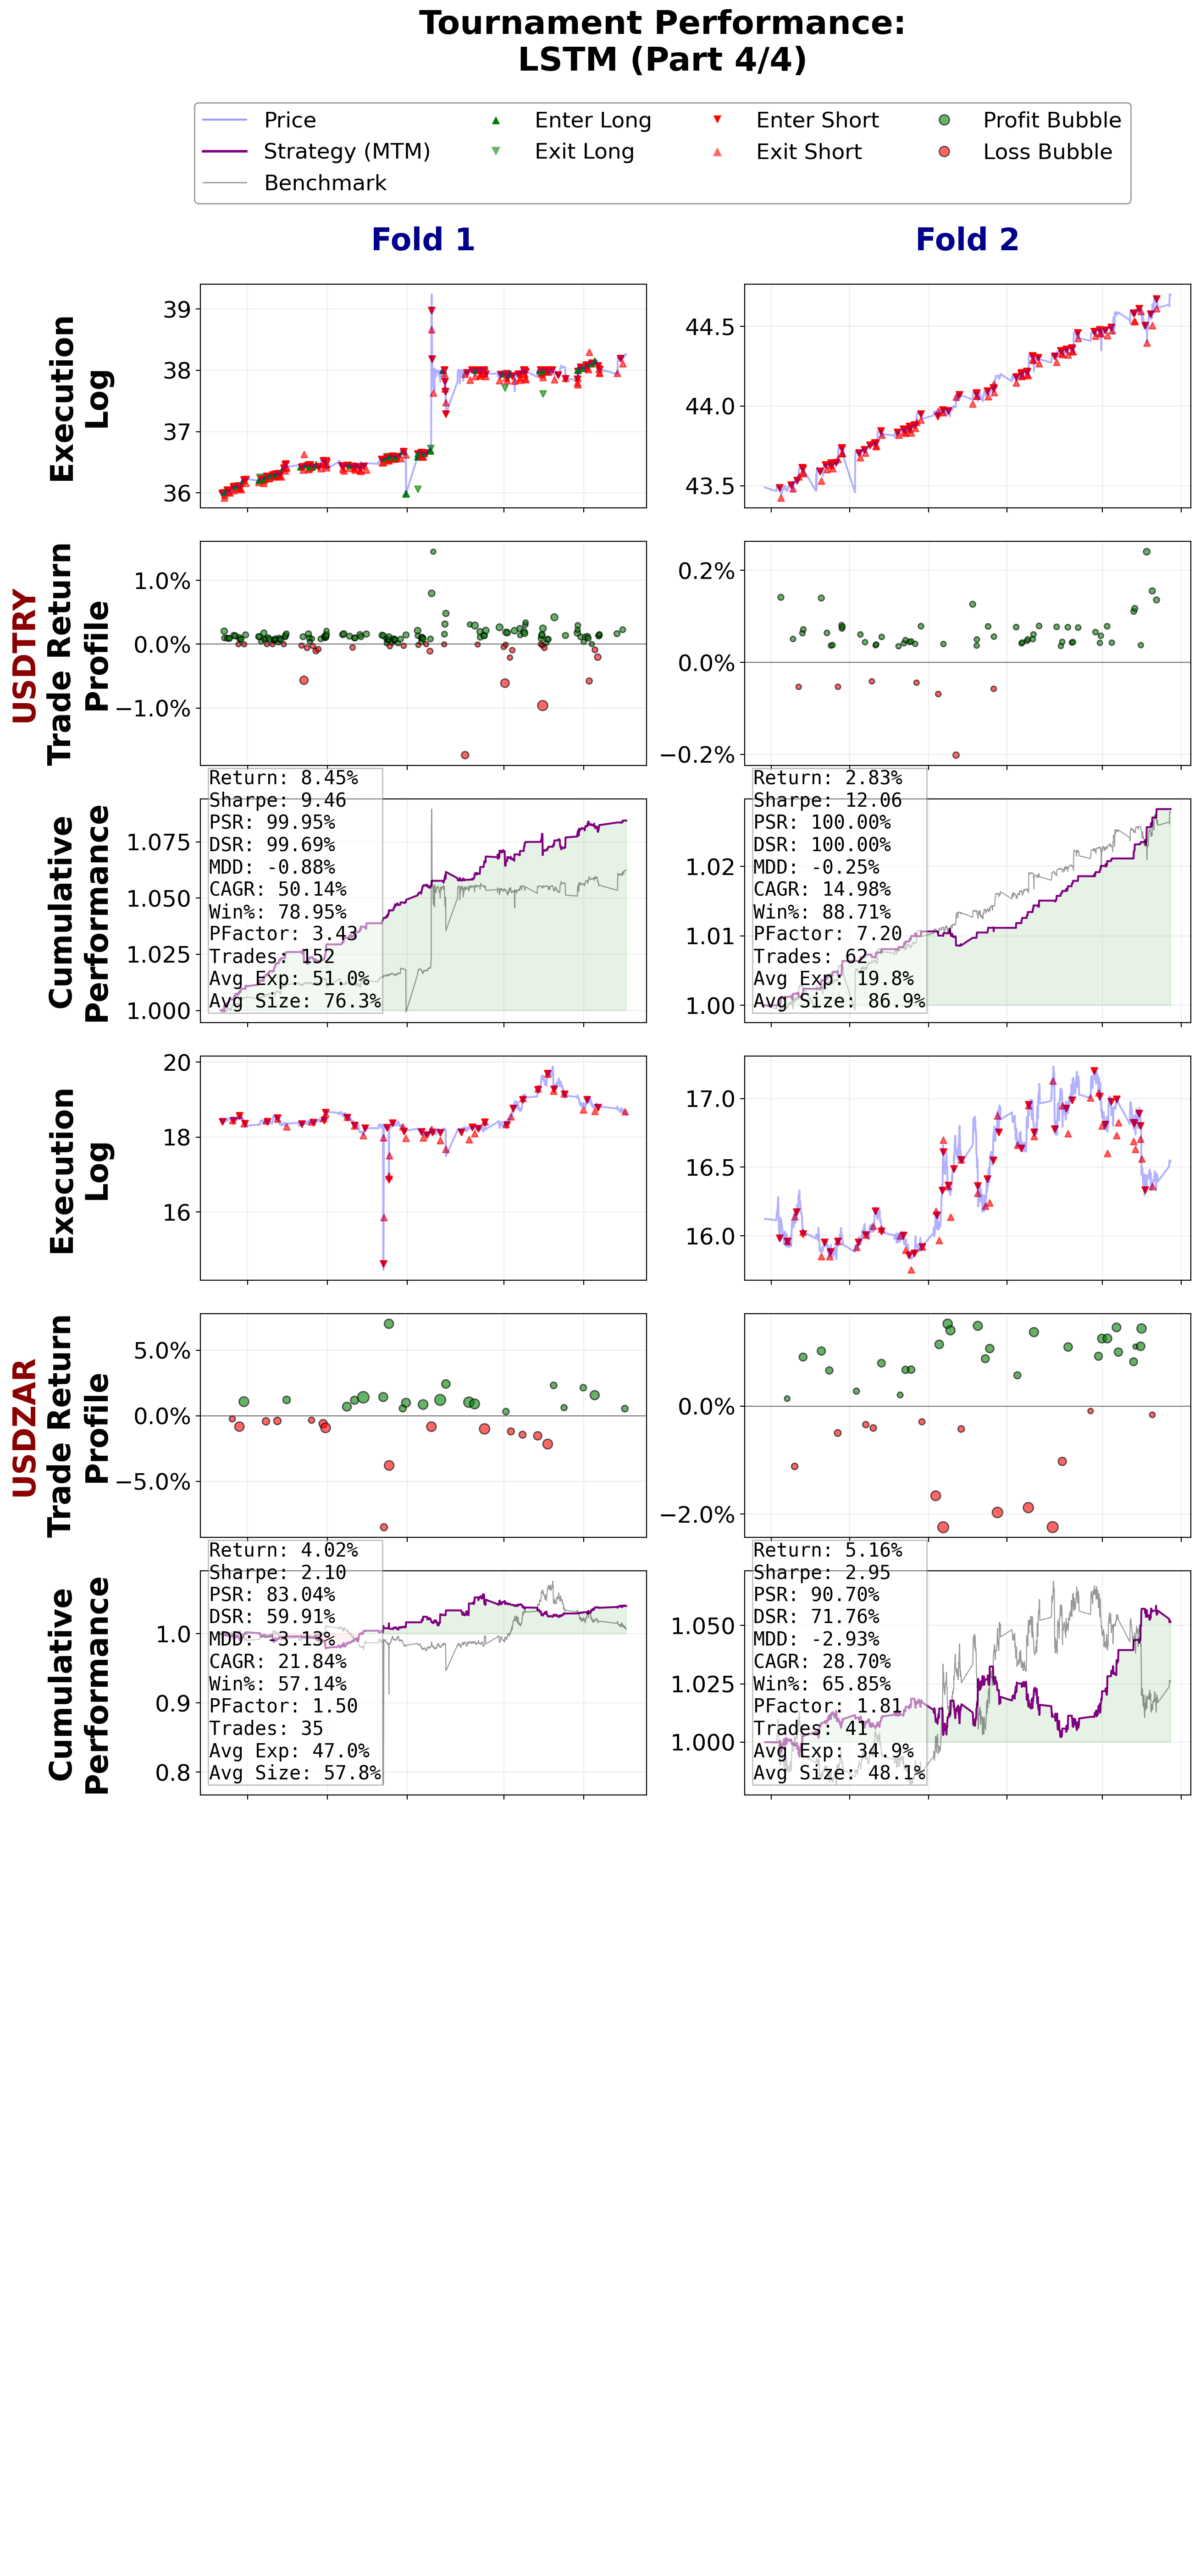
\includegraphics[width=\textwidth]{../data/figures/backtests/tournament_results_LSTM_part4.png}
        \caption{Backtest Result of LSTM During Tournament (Continued)}
        \label{fig:tournament_results_LSTM_4}
    \end{minipage}
\end{figure}


\begin{figure}[H]
    \centering
    \begin{minipage}[t]{0.49\textwidth}
        \centering
        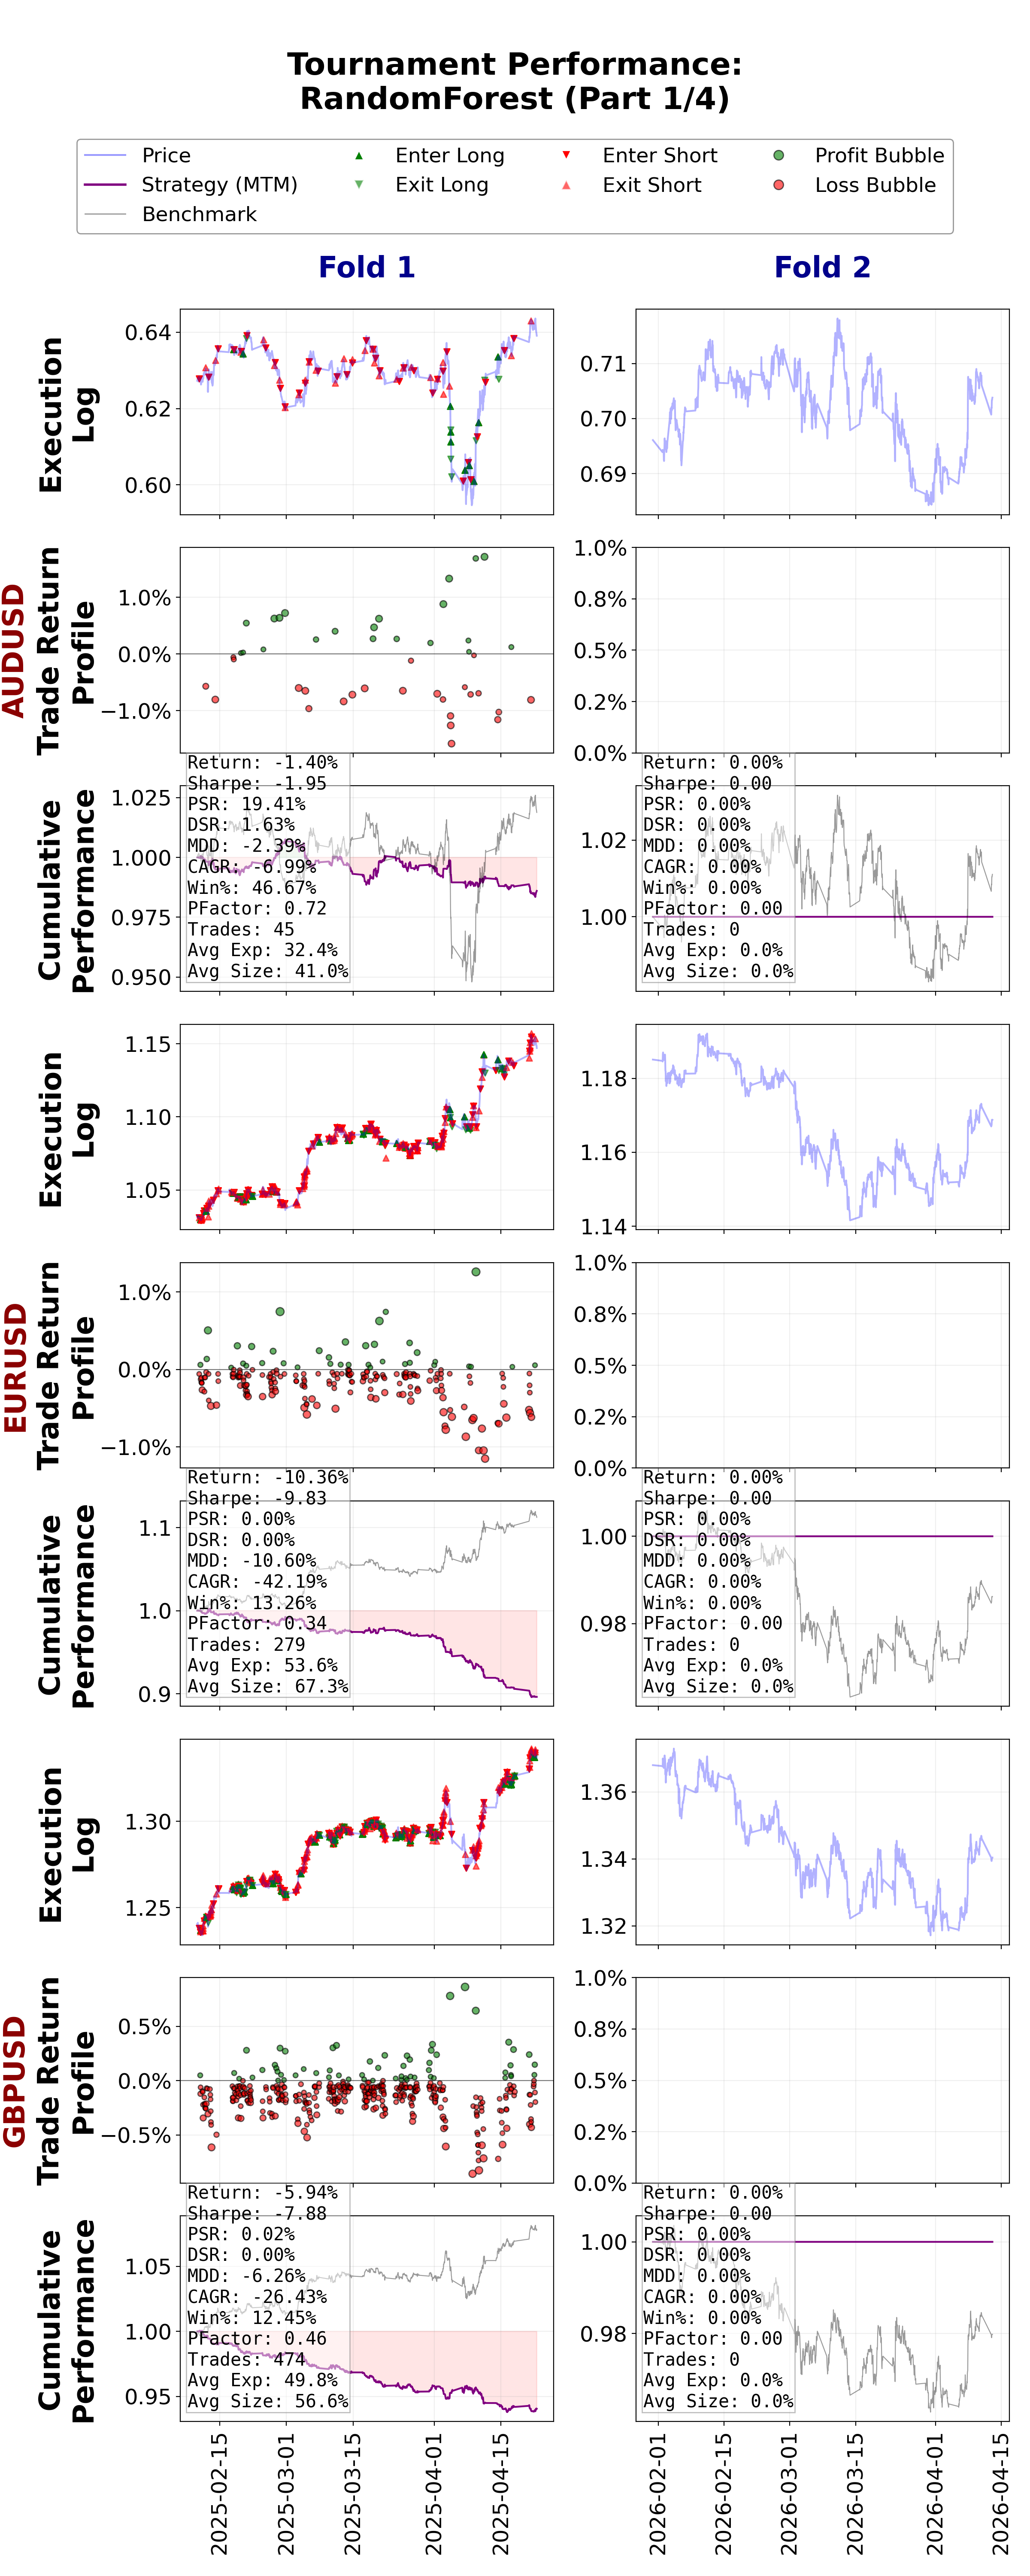
\includegraphics[width=\textwidth]{../data/figures/backtests/tournament_results_RandomForest_part1.png}
        \caption{Backtest Result of RandomForest During Tournament}
        \label{fig:tournament_result_RandomForest_1}
    \end{minipage}
    \hfill
    \begin{minipage}[t]{0.49\textwidth}
        \centering
        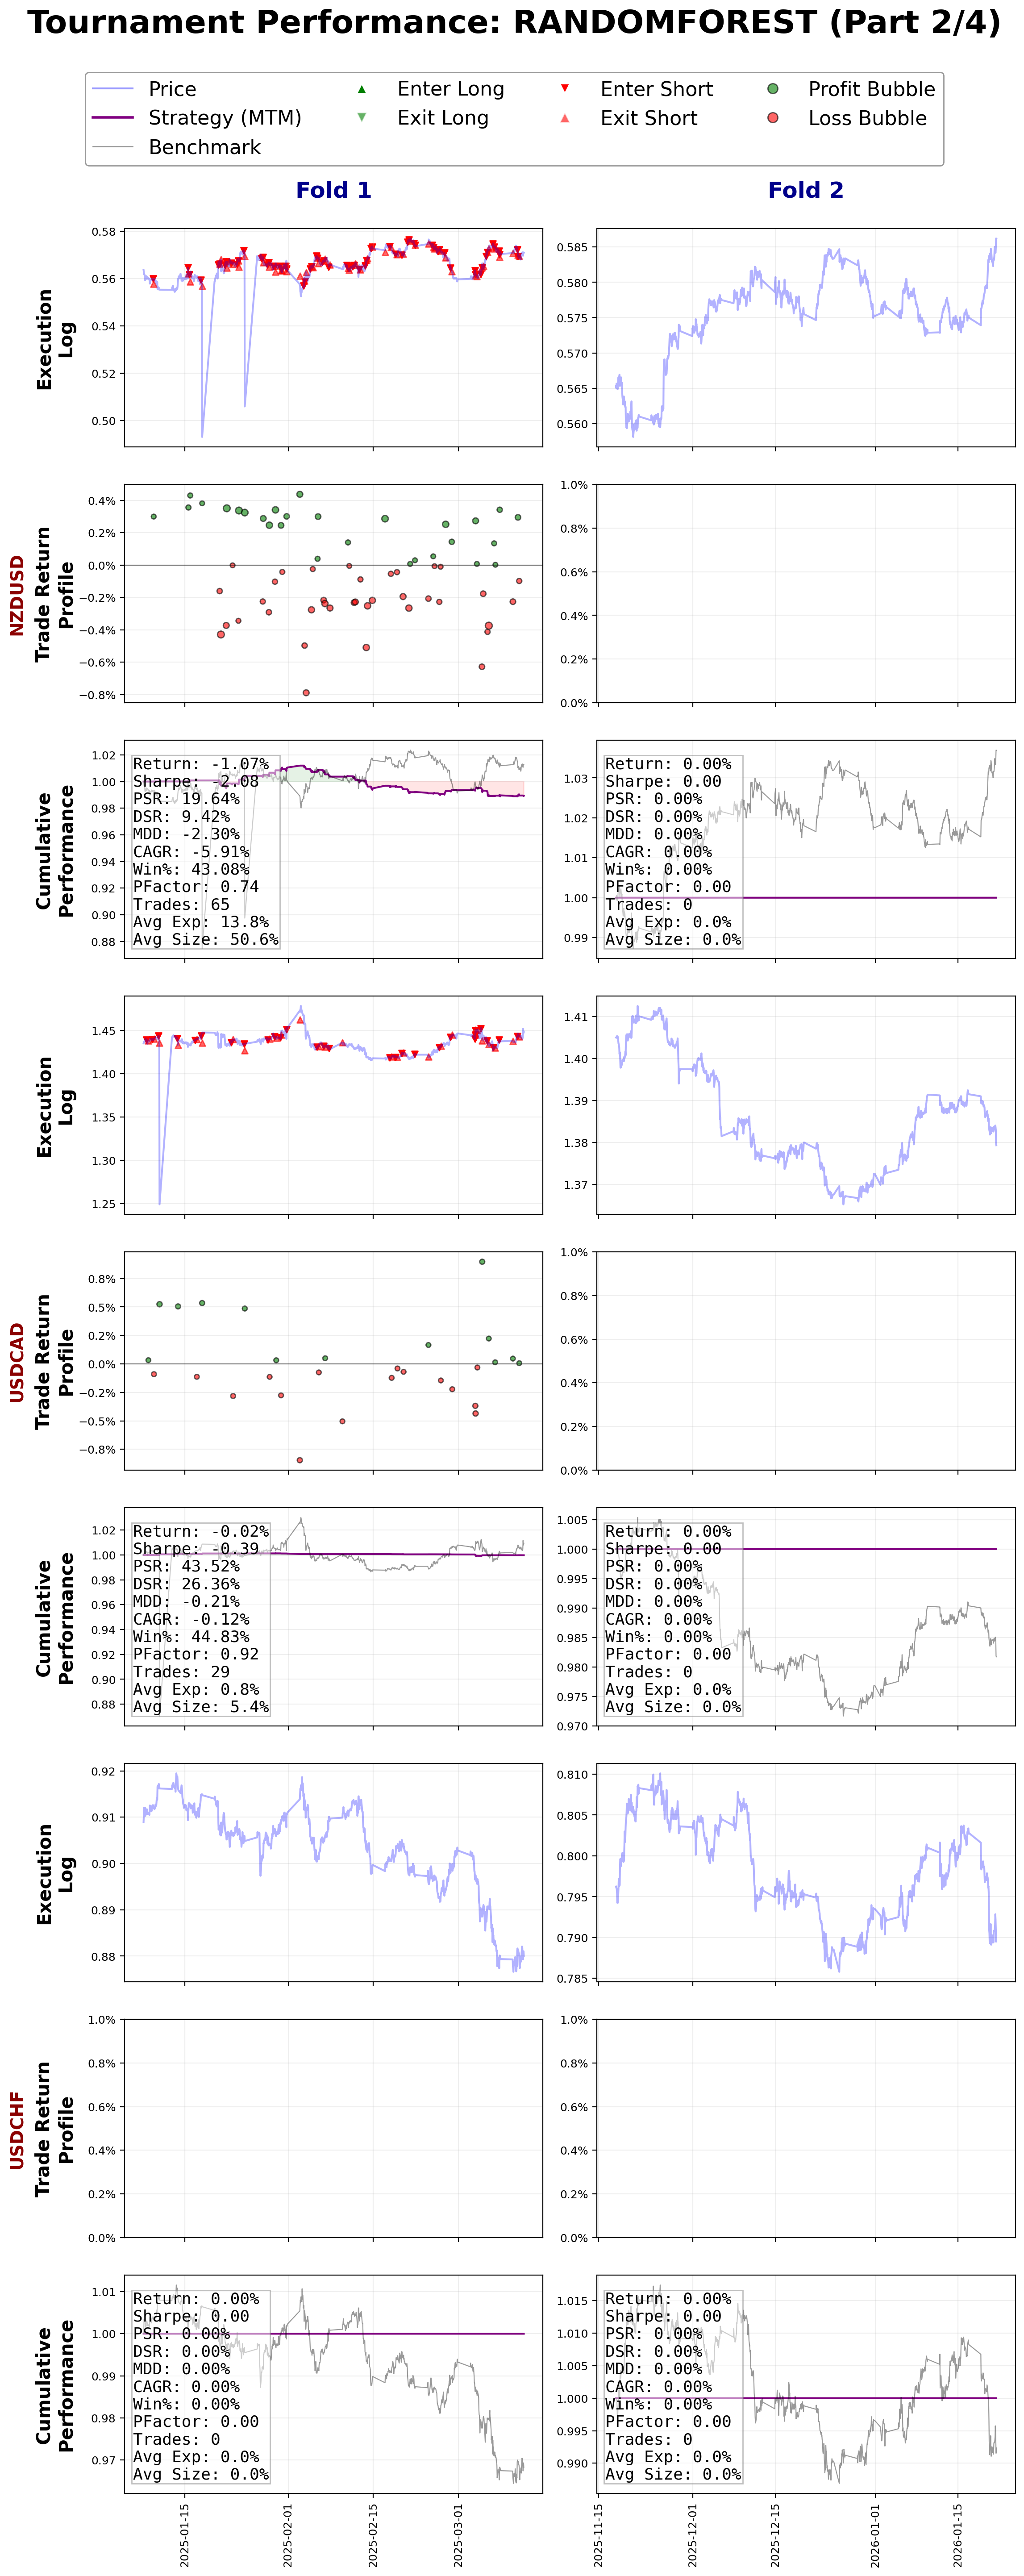
\includegraphics[width=\textwidth]{../data/figures/backtests/tournament_results_RandomForest_part2.png}
        \caption{Backtest Result of RandomForest During Tournament (Continued)}
        \label{fig:tournament_result_RandomForest_2}
    \end{minipage}
\end{figure}

\begin{figure}[H]
    \centering
    \begin{minipage}[t]{0.49\textwidth}
        \centering
        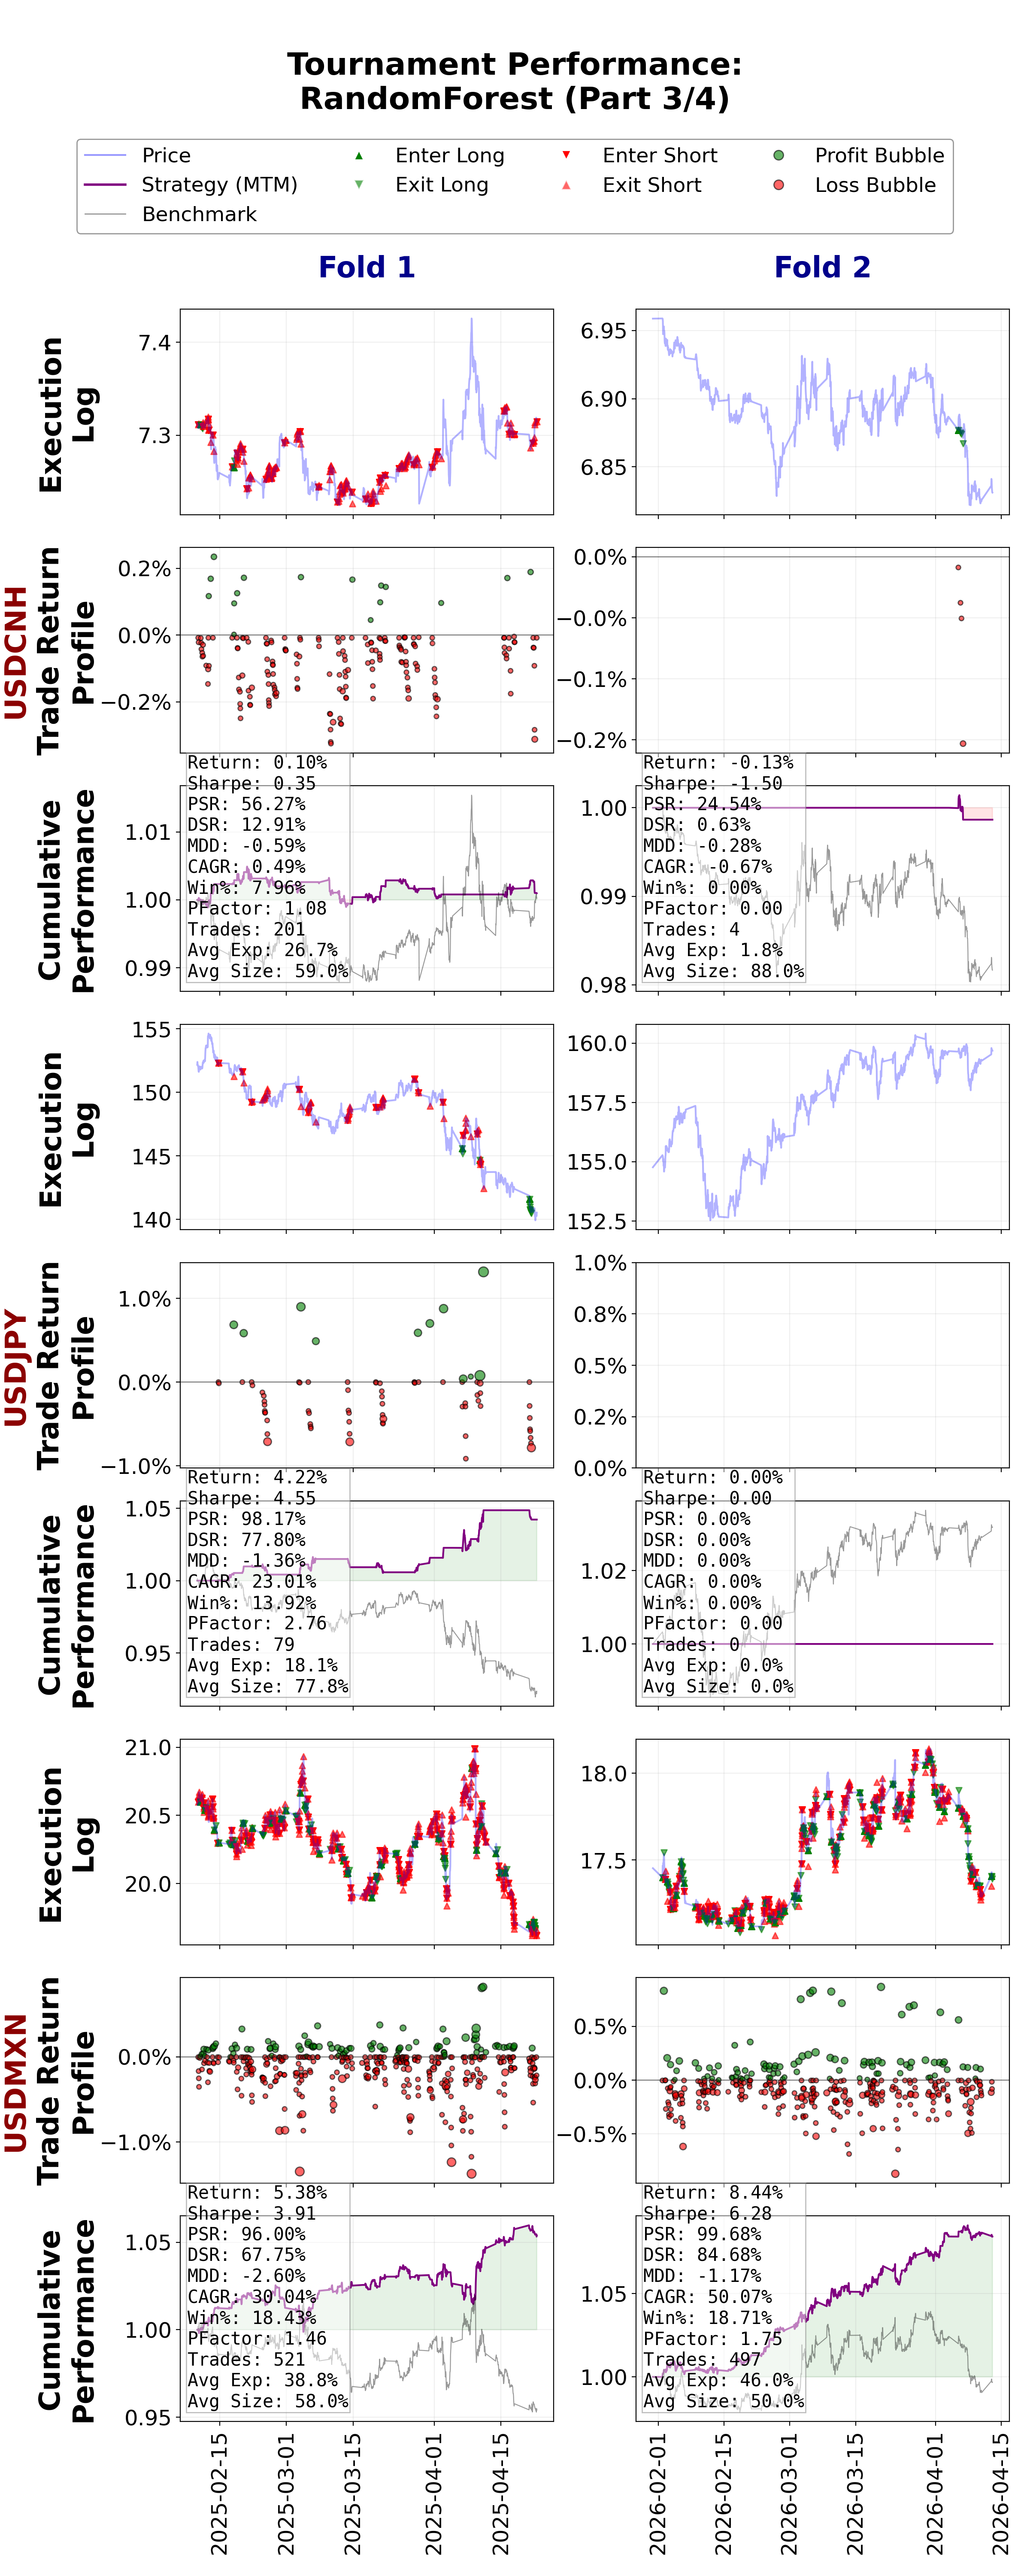
\includegraphics[width=\textwidth]{../data/figures/backtests/tournament_results_RandomForest_part3.png}
        \caption{Backtest Result of RandomForest During Tournament (Continued)}
        \label{fig:tournament_result_RandomForest_3}
    \end{minipage}
    \hfill
    \begin{minipage}[t]{0.49\textwidth}
        \centering
        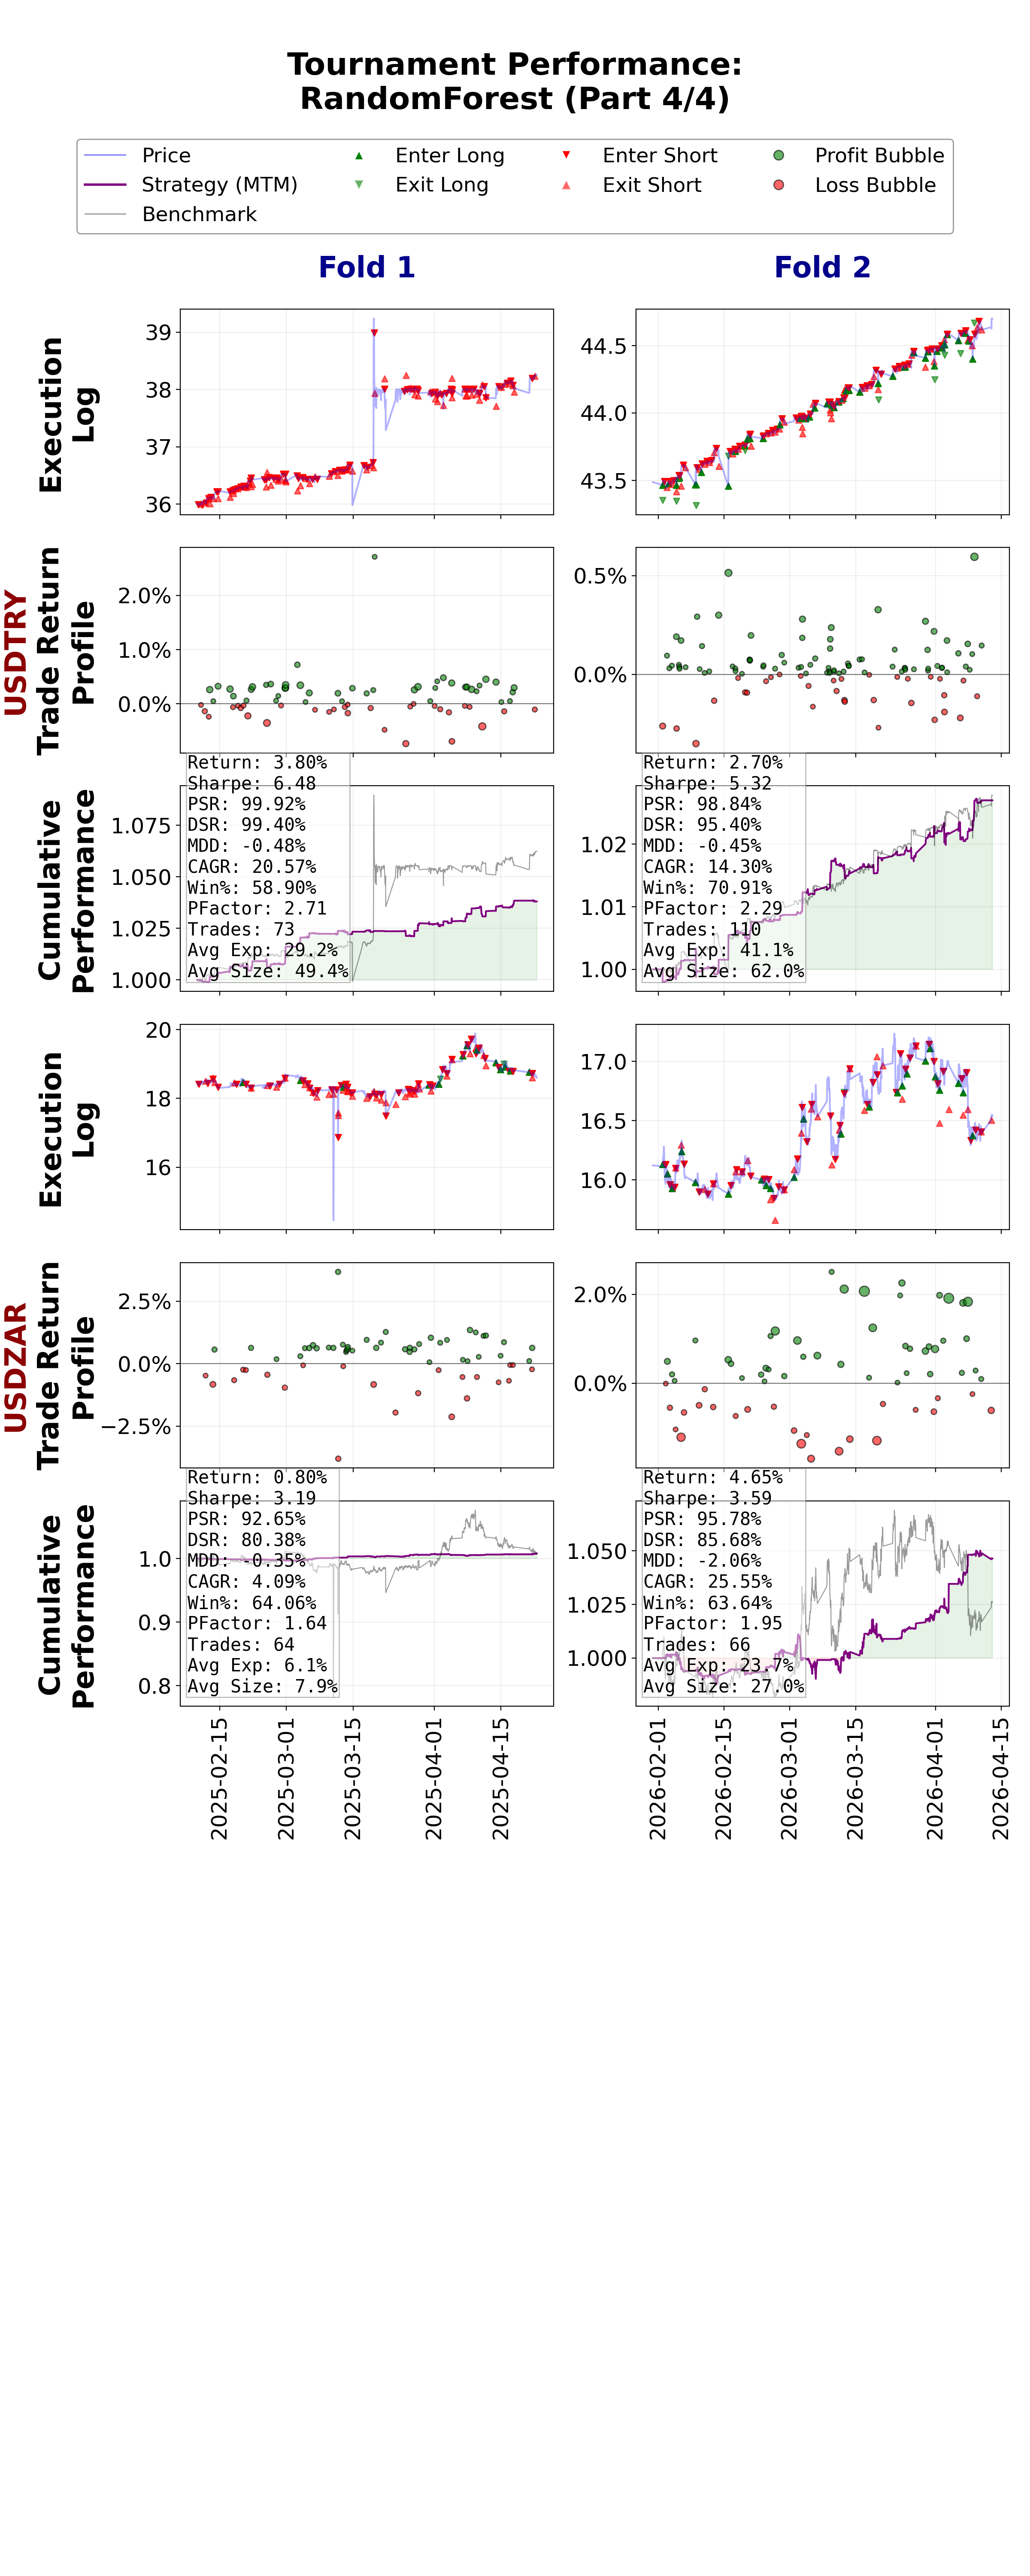
\includegraphics[width=\textwidth]{../data/figures/backtests/tournament_results_RandomForest_part4.png}
        \caption{Backtest Result of RandomForest During Tournament (Continued)}
        \label{fig:tournament_result_RandomForest_4}
    \end{minipage}
\end{figure}


\subsection{Granular Performance of Other Models}
\begin{table}[H]
\centering
\caption{{Granular Performance Analysis ExtraTrees (Tournament Phase)}}
\label{tab:perf_ExtraTrees_tournament}
\resizebox{\textwidth}{!}{\begin{tabular}{rrrrrrrrrrrrrr}
\toprule
Pair & Fold & \rotatebox{90}{Total Return (\%)} & \rotatebox{90}{Sharpe Ratio} & \rotatebox{90}{Probabilistic Sharpe (\%)} & \rotatebox{90}{Max Drawdown (\%)} & \rotatebox{90}{CAGR (\%)} & \rotatebox{90}{Win Rate (\%)} & \rotatebox{90}{Profit Factor} & \rotatebox{90}{Number of Trades} & \rotatebox{90}{Avg Capital Exposure (\%)} & \rotatebox{90}{Avg Trade Size (\%)} & \rotatebox{90}{Deflated Sharpe (\%)} & \rotatebox{90}{M2 Brier} \\
\midrule
AUDUSD & Fold 1 & -1.43\% & -2.96 & 11.64\% & -1.79\% & -7.15\% & 32.00\% & 0.60 & 50.00 & 9.88\% & 39.89\% & 3.94\% & 0.25 \\
 & Fold 2 & 0.0000\% & 0.0000 & 0.0000\% & 0.0000\% & 0.0000\% & 0.0000\% & 0.0000 & 0.0000 & 0.0000\% & 0.0000\% & 0.0000\% & 0.25 \\
EURUSD & Fold 1 & -4.10\% & -4.89 & 1.45\% & -4.48\% & -18.91\% & 37.25\% & 0.45 & 51.00 & 36.80\% & 60.11\% & 0.25\% & 0.25 \\
 & Fold 2 & 0.0000\% & 0.0000 & 0.0000\% & 0.0000\% & 0.0000\% & 0.0000\% & 0.0000 & 0.0000 & 0.0000\% & 0.0000\% & 0.0000\% & 0.25 \\
GBPUSD & Fold 1 & -1.75\% & -6.23 & 0.09\% & -1.75\% & -8.44\% & 11.11\% & 0.04 & 9.00 & 6.60\% & 71.72\% & 0.01\% & 0.25 \\
 & Fold 2 & 0.0000\% & 0.0000 & 0.0000\% & 0.0000\% & 0.0000\% & 0.0000\% & 0.0000 & 0.0000 & 0.0000\% & 0.0000\% & 0.0000\% & 0.25 \\
NZDUSD & Fold 1 & -5.47\% & -6.12 & 0.39\% & -5.51\% & -24.57\% & 25.71\% & 0.33 & 35.00 & 31.27\% & 62.59\% & 0.05\% & 0.25 \\
 & Fold 2 & 0.0000\% & 0.0000 & 0.0000\% & 0.0000\% & 0.0000\% & 0.0000\% & 0.0000 & 0.0000 & 0.0000\% & 0.0000\% & 0.0000\% & 0.25 \\
USDCAD & Fold 1 & 0.14\% & 0.19 & 53.41\% & -1.53\% & 0.70\% & 34.21\% & 1.03 & 38.00 & 35.27\% & 60.91\% & 29.38\% & 0.25 \\
 & Fold 2 & 0.0000\% & 0.0000 & 0.0000\% & 0.0000\% & 0.0000\% & 0.0000\% & 0.0000 & 0.0000 & 0.0000\% & 0.0000\% & 0.0000\% & 0.25 \\
USDCHF & Fold 1 & 0.95\% & 2.92 & 90.91\% & -0.72\% & 4.86\% & 66.67\% & 3.05 & 9.00 & 6.65\% & 45.63\% & 75.62\% & 0.25 \\
 & Fold 2 & 0.0000\% & 0.0000 & 0.0000\% & 0.0000\% & 0.0000\% & 0.0000\% & 0.0000 & 0.0000 & 0.0000\% & 0.0000\% & 0.0000\% & 0.25 \\
USDCNH & Fold 1 & 0.52\% & 2.29 & 85.80\% & -0.43\% & 2.64\% & 46.67\% & 1.38 & 75.00 & 14.92\% & 50.41\% & 66.10\% & 0.25 \\
 & Fold 2 & -0.08\% & -2.25 & 4.45\% & -0.09\% & -0.38\% & 0.0000\% & 0.0000 & 1.00 & 0.53\% & 91.00\% & 0.28\% & 0.25 \\
USDJPY & Fold 1 & 0.10\% & 3.54 & 98.93\% & -0.04\% & 0.52\% & 66.67\% & 9.64 & 3.00 & 0.14\% & 2.43\% & 91.76\% & 0.25 \\
 & Fold 2 & 0.0000\% & 0.0000 & 0.0000\% & 0.0000\% & 0.0000\% & 0.0000\% & 0.0000 & 0.0000 & 0.0000\% & 0.0000\% & 0.0000\% & 0.25 \\
USDMXN & Fold 1 & 1.37\% & 1.15 & 69.61\% & -2.75\% & 7.04\% & 54.84\% & 1.37 & 31.00 & 19.64\% & 74.07\% & 45.45\% & 0.25 \\
 & Fold 2 & -0.83\% & -1.33 & 27.64\% & -1.03\% & -4.11\% & 51.72\% & 0.77 & 58.00 & 14.14\% & 33.32\% & 10.95\% & 0.25 \\
USDTRY & Fold 1 & 4.88\% & 7.50 & 99.99\% & -0.36\% & 26.97\% & 70.00\% & 3.49 & 60.00 & 34.39\% & 51.57\% & 99.91\% & 0.25 \\
 & Fold 2 & 2.86\% & 6.28 & 97.85\% & -0.64\% & 15.20\% & 81.82\% & 4.05 & 66.00 & 30.58\% & 69.12\% & 94.12\% & 0.25 \\
USDZAR & Fold 1 & -0.52\% & -2.45 & 10.34\% & -0.76\% & -2.57\% & 33.33\% & 0.31 & 6.00 & 0.86\% & 27.33\% & 2.37\% & 0.25 \\
 & Fold 2 & 0.16\% & 2.64 & 89.55\% & -0.07\% & 0.83\% & 85.71\% & 16.09 & 7.00 & 0.68\% & 7.31\% & 71.85\% & 0.25 \\
\midrule
\midrule
Fold 1 Avg &  & \shortstack{-0.48\% \\ $\pm$ 2.76\%} & \shortstack{-0.46 \\ $\pm$ 4.43} & \shortstack{47.51\% \\ $\pm$ 43.05\%} & \shortstack{-1.83\% \\ $\pm$ 1.77\%} & \shortstack{-1.72\% \\ $\pm$ 13.66\%} & \shortstack{43.50\% \\ $\pm$ 19.08\%} & \shortstack{1.97 \\ $\pm$ 2.78} & \shortstack{33.36 \\ $\pm$ 24.33} & \shortstack{17.86\% \\ $\pm$ 14.30\%} & \shortstack{49.70\% \\ $\pm$ 20.81\%} & \shortstack{37.71\% \\ $\pm$ 39.74\%} & \shortstack{0.25 \\ $\pm$ 0.0000} \\
Fold 2 Avg &  & \shortstack{0.19\% \\ $\pm$ 0.92\%} & \shortstack{0.49 \\ $\pm$ 2.25} & \shortstack{19.95\% \\ $\pm$ 37.41\%} & \shortstack{-0.17\% \\ $\pm$ 0.34\%} & \shortstack{1.05\% \\ $\pm$ 4.86\%} & \shortstack{19.93\% \\ $\pm$ 35.14\%} & \shortstack{1.90 \\ $\pm$ 4.86} & \shortstack{12.00 \\ $\pm$ 24.87} & \shortstack{4.18\% \\ $\pm$ 9.72\%} & \shortstack{18.25\% \\ $\pm$ 32.49\%} & \shortstack{16.11\% \\ $\pm$ 33.60\%} & \shortstack{0.25 \\ $\pm$ 0.0000} \\
Total Avg &  & \shortstack{-0.14\% \\ $\pm$ 2.04\%} & \shortstack{0.01 \\ $\pm$ 3.46} & \shortstack{33.73\% \\ $\pm$ 41.81\%} & \shortstack{-1.00\% \\ $\pm$ 1.51\%} & \shortstack{-0.34\% \\ $\pm$ 10.11\%} & \shortstack{31.71\% \\ $\pm$ 30.11\%} & \shortstack{1.94 \\ $\pm$ 3.86} & \shortstack{22.68 \\ $\pm$ 26.38} & \shortstack{11.02\% \\ $\pm$ 13.83\%} & \shortstack{33.97\% \\ $\pm$ 31.11\%} & \shortstack{26.91\% \\ $\pm$ 37.57\%} & \shortstack{0.25 \\ $\pm$ 0.0027} \\
\bottomrule
\end{tabular}}
\end{table}

\begin{table}[H]
\centering
\caption{{Granular Performance Analysis GRU (Tournament Phase)}}
\label{tab:perf_GRU_tournament}
\resizebox{\textwidth}{!}{\begin{tabular}{rrrrrrrrrrrrrr}
\toprule
Pair & Fold & \rotatebox{90}{Total Return (\%)} & \rotatebox{90}{Sharpe Ratio} & \rotatebox{90}{Probabilistic Sharpe (\%)} & \rotatebox{90}{Max Drawdown (\%)} & \rotatebox{90}{CAGR (\%)} & \rotatebox{90}{Win Rate (\%)} & \rotatebox{90}{Profit Factor} & \rotatebox{90}{Number of Trades} & \rotatebox{90}{Avg Capital Exposure (\%)} & \rotatebox{90}{Avg Trade Size (\%)} & \rotatebox{90}{Deflated Sharpe (\%)} & \rotatebox{90}{M2 Brier} \\
\midrule
AUDUSD & Fold 1 & -0.10\% & -0.98 & 33.27\% & -0.22\% & -0.54\% & 68.42\% & 0.80 & 19.00 & 2.93\% & 9.52\% & 2.23\% & 0.25 \\
 & Fold 2 & 0.0000\% & 0.0000 & 0.0000\% & 0.0000\% & 0.0000\% & 0.0000\% & 0.0000 & 0.0000 & 0.0000\% & 0.0000\% & 0.0000\% & 0.25 \\
EURUSD & Fold 1 & -1.34\% & -3.63 & 4.58\% & -1.65\% & -6.53\% & 37.50\% & 0.15 & 8.00 & 4.47\% & 34.38\% & 0.04\% & 0.25 \\
 & Fold 2 & 0.0000\% & 0.0000 & 0.0000\% & 0.0000\% & 0.0000\% & 0.0000\% & 0.0000 & 0.0000 & 0.0000\% & 0.0000\% & 0.0000\% & 0.25 \\
GBPUSD & Fold 1 & -2.93\% & -6.32 & 0.28\% & -2.94\% & -13.82\% & 11.11\% & 0.17 & 18.00 & 12.47\% & 61.45\% & 0.0000\% & 0.25 \\
 & Fold 2 & 0.0000\% & 0.0000 & 0.0000\% & 0.0000\% & 0.0000\% & 0.0000\% & 0.0000 & 0.0000 & 0.0000\% & 0.0000\% & 0.0000\% & 0.25 \\
NZDUSD & Fold 1 & -1.62\% & -1.42 & 26.45\% & -3.34\% & -7.86\% & 48.00\% & 0.77 & 25.00 & 37.96\% & 83.31\% & 1.34\% & 0.25 \\
 & Fold 2 & -1.06\% & -2.18 & 16.27\% & -1.33\% & -5.19\% & 37.50\% & 0.60 & 24.00 & 8.13\% & 68.14\% & 0.31\% & 0.25 \\
USDCAD & Fold 1 & -1.05\% & -2.44 & 13.85\% & -1.54\% & -5.13\% & 51.85\% & 0.61 & 27.00 & 25.18\% & 38.33\% & 0.37\% & 0.25 \\
 & Fold 2 & 0.0000\% & 0.0000 & 0.0000\% & 0.0000\% & 0.0000\% & 0.0000\% & 0.0000 & 0.0000 & 0.0000\% & 0.0000\% & 0.0000\% & 0.25 \\
USDCHF & Fold 1 & 1.43\% & 3.44 & 95.22\% & -0.49\% & 7.36\% & 48.57\% & 2.14 & 35.00 & 14.63\% & 56.98\% & 47.29\% & 0.25 \\
 & Fold 2 & -0.06\% & -0.40 & 42.88\% & -0.45\% & -0.28\% & 78.57\% & 0.90 & 14.00 & 4.18\% & 21.91\% & 2.75\% & 0.25 \\
USDCNH & Fold 1 & -0.11\% & -0.50 & 41.15\% & -0.69\% & -0.55\% & 30.77\% & 0.86 & 13.00 & 12.32\% & 88.41\% & 3.52\% & 0.25 \\
 & Fold 2 & 0.91\% & 3.94 & 97.20\% & -0.41\% & 4.65\% & 75.00\% & 2.64 & 16.00 & 15.31\% & 68.71\% & 51.16\% & 0.25 \\
USDJPY & Fold 1 & 19.83\% & 1.36 & 72.87\% & -61.36\% & 147.60\% & 55.88\% & 1.15 & 34.00 & 951.31\% & 1489.28\% & 16.17\% & 0.25 \\
 & Fold 2 & -6.54\% & -0.24 & 45.76\% & -21.79\% & -28.76\% & 63.64\% & 0.92 & 44.00 & 468.20\% & 1539.82\% & 3.31\% & 0.25 \\
USDMXN & Fold 1 & 14.82\% & 4.84 & 98.45\% & -6.30\% & 99.88\% & 58.67\% & 1.76 & 75.00 & 61.45\% & 196.74\% & 71.37\% & 0.25 \\
 & Fold 2 & 34.87\% & 7.54 & 99.94\% & -3.59\% & 347.70\% & 64.53\% & 1.96 & 172.00 & 145.23\% & 148.94\% & 94.18\% & 0.25 \\
USDTRY & Fold 1 & 32.34\% & 4.48 & 95.62\% & -17.13\% & 307.16\% & 78.82\% & 1.79 & 170.00 & 262.09\% & 324.79\% & 63.49\% & 0.25 \\
 & Fold 2 & 43.01\% & 13.62 & 99.98\% & -3.93\% & 500.61\% & 94.25\% & 5.52 & 174.00 & 269.81\% & 391.88\% & 99.43\% & 0.25 \\
USDZAR & Fold 1 & 37.09\% & 4.64 & 99.44\% & -5.61\% & 386.44\% & 57.97\% & 1.79 & 138.00 & 148.92\% & 154.83\% & 72.02\% & 0.25 \\
 & Fold 2 & 48.37\% & 7.45 & 99.94\% & -5.41\% & 621.97\% & 63.83\% & 2.09 & 141.00 & 136.94\% & 140.67\% & 94.03\% & 0.25 \\
\midrule
\midrule
Fold 1 Avg &  & \shortstack{8.94\% \\ $\pm$ 14.73\%} & \shortstack{0.32 \\ $\pm$ 3.74} & \shortstack{52.83\% \\ $\pm$ 40.13\%} & \shortstack{-9.21\% \\ $\pm$ 17.95\%} & \shortstack{83.09\% \\ $\pm$ 141.38\%} & \shortstack{49.78\% \\ $\pm$ 18.41\%} & \shortstack{1.09 \\ $\pm$ 0.69} & \shortstack{51.09 \\ $\pm$ 54.32} & \shortstack{139.43\% \\ $\pm$ 280.79\%} & \shortstack{230.73\% \\ $\pm$ 427.21\%} & \shortstack{25.26\% \\ $\pm$ 31.32\%} & \shortstack{0.25 \\ $\pm$ 0.0000} \\
Fold 2 Avg &  & \shortstack{10.86\% \\ $\pm$ 20.38\%} & \shortstack{2.70 \\ $\pm$ 4.88} & \shortstack{45.63\% \\ $\pm$ 45.51\%} & \shortstack{-3.36\% \\ $\pm$ 6.41\%} & \shortstack{130.97\% \\ $\pm$ 238.86\%} & \shortstack{43.39\% \\ $\pm$ 36.96\%} & \shortstack{1.33 \\ $\pm$ 1.68} & \shortstack{53.18 \\ $\pm$ 71.83} & \shortstack{95.25\% \\ $\pm$ 152.43\%} & \shortstack{216.37\% \\ $\pm$ 454.03\%} & \shortstack{31.38\% \\ $\pm$ 44.05\%} & \shortstack{0.25 \\ $\pm$ 0.0000} \\
Total Avg &  & \shortstack{9.90\% \\ $\pm$ 17.38\%} & \shortstack{1.51 \\ $\pm$ 4.41} & \shortstack{49.23\% \\ $\pm$ 42.03\%} & \shortstack{-6.28\% \\ $\pm$ 13.49\%} & \shortstack{107.03\% \\ $\pm$ 193.10\%} & \shortstack{46.59\% \\ $\pm$ 28.68\%} & \shortstack{1.21 \\ $\pm$ 1.26} & \shortstack{52.14 \\ $\pm$ 62.15} & \shortstack{117.34\% \\ $\pm$ 221.63\%} & \shortstack{223.55\% \\ $\pm$ 430.26\%} & \shortstack{28.32\% \\ $\pm$ 37.43\%} & \shortstack{0.25 \\ $\pm$ 0.0017} \\
\bottomrule
\end{tabular}}
\end{table}

\begin{sidewaystable}
\centering
\caption{{Granular Performance Analysis LightGBM (Tournament Phase)}}
\label{tab:perf_LightGBM_tournament}
\resizebox{\textwidth}{!}{\begin{tabular}{llllllllllllllll}
\toprule
Fold & Metric & AUDUSD & EURUSD & GBPUSD & NZDUSD & USDCAD & USDCHF & USDCNH & USDJPY & USDMXN & USDTRY & USDZAR & Average & StDev & Interpretation \\
\midrule
Fold 1 & total return & 0.0055 & -0.02 & -0.04 & -0.0005 & -0.0029 & 0.0009 & 0.0073 & -0.0053 & -0.0056 & 0.09 & 0.03 & 0.0058 & 0.03 &  \\
 & sharpe & 0.98 & -3.75 & -5.04 & -0.13 & -0.27 & 0.51 & 3.38 & -1.09 & -1.37 & 20.11 & 4.28 & 1.60 & 6.39 &  \\
 & probabilistic sharpe & 0.66 & 0.05 & 0.02 & 0.48 & 0.45 & 0.59 & 0.93 & 0.32 & 0.28 & 1.00 & 0.97 & 0.52 & 0.33 &  \\
 & min trl & 16509.00 & inf & inf & inf & inf & 56241.00 & 1277.00 & inf & inf & 46.00 & 866.00 & inf & nan &  \\
 & max dd & -0.02 & -0.02 & -0.05 & -0.01 & -0.03 & -0.0025 & -0.0056 & -0.01 & -0.0092 & -0.0030 & -0.0099 & -0.02 & 0.01 &  \\
 & cagr & 0.03 & -0.09 & -0.22 & -0.0028 & -0.02 & 0.0050 & 0.04 & -0.03 & -0.03 & 0.66 & 0.18 & 0.05 & 0.21 &  \\
 & win rate & 0.53 & 0.60 & 0.59 & 0.77 & 0.55 & 0.25 & 0.64 & 0.56 & 0.42 & 0.91 & 0.72 & 0.60 & 0.17 &  \\
 & profit factor & 1.19 & 0.59 & 0.51 & 0.99 & 0.91 & 1.13 & 1.96 & 0.86 & 0.74 & 7.10 & 2.26 & 1.66 & 1.80 &  \\
 & n trades & 51.00 & 80.00 & 71.00 & 57.00 & 31.00 & 20.00 & 39.00 & 71.00 & 57.00 & 174.00 & 47.00 & 63.45 & 38.91 &  \\
 & avg capital exposure & 18.79 & 19.14 & 50.09 & 11.96 & 34.20 & 2.43 & 11.67 & 16.15 & 10.45 & 45.24 & 17.06 & 21.56 & 14.39 &  \\
 & avg trade size & 32.67 & 28.58 & 71.74 & 27.98 & 46.27 & 27.48 & 59.08 & 38.72 & 15.10 & 56.55 & 31.36 & 39.59 & 16.14 &  \\
 & deflated sharpe & 0.37 & 0.0083 & 0.0017 & 0.21 & 0.19 & 0.29 & 0.76 & 0.11 & 0.09 & 1.00 & 0.86 & 0.35 & 0.34 &  \\
 & deflated min trl & inf & inf & inf & inf & inf & inf & 5765.00 & inf & inf & 55.00 & 2555.00 & inf & nan &  \\
 & pfdr & 1.00 & 1.00 & 1.00 & 1.00 & 1.00 & 1.00 & 1.00 & 1.00 & 1.00 & 1.00 & 1.00 & 1.00 & 0.0000 &  \\
 & m2 brier & 0.25 & 0.25 & 0.25 & 0.25 & 0.25 & 0.25 & 0.25 & 0.25 & 0.25 & 0.25 & 0.25 & 0.25 & 0.0000 &  \\
Fold 2 & total return & 0.0000 & 0.0000 & 0.0000 & 0.0000 & 0.0000 & 0.0000 & 0.0006 & 0.0000 & 0.0046 & 0.03 & 0.05 & 0.0080 & 0.02 &  \\
 & sharpe & 0.0000 & 0.0000 & 0.0000 & 0.0000 & 0.0000 & 0.0000 & 0.47 & 0.0000 & 1.88 & 13.76 & 8.71 & 2.26 & 4.40 &  \\
 & probabilistic sharpe & 0.0000 & 0.0000 & 0.0000 & 0.0000 & 0.0000 & 0.0000 & 0.58 & 0.0000 & 0.79 & 1.00 & 1.00 & 0.31 & 0.42 &  \\
 & min trl & inf & inf & inf & inf & inf & inf & 73690.00 & inf & 4625.00 & 149.00 & 200.00 & inf & nan &  \\
 & max dd & 0.0000 & 0.0000 & 0.0000 & 0.0000 & 0.0000 & 0.0000 & -0.0019 & 0.0000 & -0.0040 & -0.0022 & -0.0040 & -0.0011 & 0.0016 &  \\
 & cagr & 0.0000 & 0.0000 & 0.0000 & 0.0000 & 0.0000 & 0.0000 & 0.0034 & 0.0000 & 0.03 & 0.19 & 0.33 & 0.05 & 0.10 &  \\
 & win rate & 0.0000 & 0.0000 & 0.0000 & 0.0000 & 0.0000 & 0.0000 & 0.63 & 0.0000 & 0.58 & 0.87 & 0.80 & 0.26 & 0.35 &  \\
 & profit factor & 0.0000 & 0.0000 & 0.0000 & 0.0000 & 0.0000 & 0.0000 & 1.14 & 0.0000 & 1.66 & 4.32 & 5.22 & 1.12 & 1.81 &  \\
 & n trades & 0.0000 & 0.0000 & 0.0000 & 0.0000 & 0.0000 & 0.0000 & 27.00 & 0.0000 & 71.00 & 156.00 & 74.00 & 29.82 & 48.43 &  \\
 & avg capital exposure & 0.0000 & 0.0000 & 0.0000 & 0.0000 & 0.0000 & 0.0000 & 12.18 & 0.0000 & 20.30 & 28.14 & 31.51 & 8.38 & 11.96 &  \\
 & avg trade size & 0.0000 & 0.0000 & 0.0000 & 0.0000 & 0.0000 & 0.0000 & 90.41 & 0.0000 & 21.15 & 40.90 & 48.05 & 18.23 & 28.52 &  \\
 & deflated sharpe & 0.0000 & 0.0000 & 0.0000 & 0.0000 & 0.0000 & 0.0000 & 0.29 & 0.0000 & 0.51 & 1.00 & 1.00 & 0.25 & 0.39 &  \\
 & deflated min trl & inf & inf & inf & inf & inf & inf & inf & inf & 2780474.00 & 197.00 & 317.00 & inf & nan &  \\
 & pfdr & 1.00 & 1.00 & 1.00 & 1.00 & 1.00 & 1.00 & 1.00 & 1.00 & 1.00 & 1.00 & 1.00 & 1.00 & 0.0000 &  \\
 & m2 brier & 0.25 & 0.25 & 0.25 & 0.25 & 0.25 & 0.25 & 0.25 & 0.25 & 0.25 & 0.25 & 0.25 & 0.25 & 0.0000 &  \\
\bottomrule
\end{tabular}}
\end{sidewaystable}

\begin{table}[H]
\centering
\caption{{Granular Performance Analysis LSTM (Tournament Phase)}}
\label{tab:perf_LSTM_tournament}
\resizebox{\textwidth}{!}{\begin{tabular}{rrrrrrrrrrrrrr}
\toprule
Pair & Fold & \rotatebox{90}{Total Return (\%)} & \rotatebox{90}{Sharpe Ratio} & \rotatebox{90}{Probabilistic Sharpe (\%)} & \rotatebox{90}{Max Drawdown (\%)} & \rotatebox{90}{CAGR (\%)} & \rotatebox{90}{Win Rate (\%)} & \rotatebox{90}{Profit Factor} & \rotatebox{90}{Number of Trades} & \rotatebox{90}{Avg Capital Exposure (\%)} & \rotatebox{90}{Avg Trade Size (\%)} & \rotatebox{90}{Deflated Sharpe (\%)} & \rotatebox{90}{M2 Brier} \\
\midrule
AUDUSD & Fold 1 & -0.88\% & -2.14 & 17.17\% & -1.44\% & -4.44\% & 26.67\% & 0.50 & 15.00 & 8.06\% & 34.96\% & 6.54\% & 0.25 \\
 & Fold 2 & 0.0000\% & 0.0000 & 0.0000\% & 0.0000\% & 0.0000\% & 0.0000\% & 0.0000 & 0.0000 & 0.0000\% & 0.0000\% & 0.0000\% & 0.25 \\
EURUSD & Fold 1 & -0.02\% & -1.27 & 29.39\% & -0.02\% & -0.08\% & 0.0000\% & 0.0000 & 1.00 & 0.05\% & 2.88\% & 13.95\% & 0.25 \\
 & Fold 2 & -0.05\% & -0.88 & 35.47\% & -0.16\% & -0.26\% & 31.82\% & 0.77 & 22.00 & 1.22\% & 11.16\% & 7.68\% & 0.25 \\
GBPUSD & Fold 1 & -0.26\% & -5.56 & 0.64\% & -0.27\% & -1.32\% & 19.23\% & 0.12 & 26.00 & 0.95\% & 8.85\% & 0.11\% & 0.25 \\
 & Fold 2 & 0.0000\% & 0.0000 & 0.0000\% & 0.0000\% & 0.0000\% & 0.0000\% & 0.0000 & 0.0000 & 0.0000\% & 0.0000\% & 0.0000\% & 0.25 \\
NZDUSD & Fold 1 & -0.27\% & -0.37 & 43.47\% & -1.69\% & -1.36\% & 61.29\% & 0.89 & 31.00 & 21.11\% & 43.48\% & 23.25\% & 0.25 \\
 & Fold 2 & 0.0000\% & 0.0000 & 0.0000\% & 0.0000\% & 0.0000\% & 0.0000\% & 0.0000 & 0.0000 & 0.0000\% & 0.0000\% & 0.0000\% & 0.25 \\
USDCAD & Fold 1 & 2.30\% & 2.22 & 84.28\% & -1.90\% & 12.05\% & 51.52\% & 1.73 & 33.00 & 59.78\% & 65.47\% & 66.63\% & 0.25 \\
 & Fold 2 & 0.0000\% & 0.0000 & 0.0000\% & 0.0000\% & 0.0000\% & 0.0000\% & 0.0000 & 0.0000 & 0.0000\% & 0.0000\% & 0.0000\% & 0.25 \\
USDCHF & Fold 1 & 0.45\% & 4.79 & 99.31\% & -0.09\% & 2.25\% & 71.43\% & 7.49 & 21.00 & 1.88\% & 8.48\% & 96.49\% & 0.25 \\
 & Fold 2 & 0.02\% & 1.95 & 86.10\% & -0.02\% & 0.12\% & 100.00\% & inf & 1.00 & 0.10\% & 4.19\% & 38.22\% & 0.25 \\
USDCNH & Fold 1 & 0.58\% & 1.29 & 71.63\% & -0.83\% & 2.95\% & 52.94\% & 1.19 & 68.00 & 37.88\% & 50.54\% & 50.38\% & 0.25 \\
 & Fold 2 & 0.22\% & 3.38 & 94.25\% & -0.10\% & 1.11\% & 51.72\% & 2.65 & 29.00 & 2.62\% & 20.14\% & 65.98\% & 0.25 \\
USDJPY & Fold 1 & 0.0000\% & 0.0000 & 0.0000\% & 0.0000\% & 0.0000\% & 0.0000\% & 0.0000 & 0.0000 & 0.0000\% & 0.0000\% & 0.0000\% & 0.25 \\
 & Fold 2 & 0.0000\% & 0.0000 & 0.0000\% & 0.0000\% & 0.0000\% & 0.0000\% & 0.0000 & 0.0000 & 0.0000\% & 0.0000\% & 0.0000\% & 0.25 \\
USDMXN & Fold 1 & -0.01\% & -0.25 & 45.63\% & -0.12\% & -0.06\% & 60.00\% & 0.90 & 5.00 & 0.29\% & 8.02\% & 24.96\% & 0.25 \\
 & Fold 2 & -0.0021\% & -3.07 & 6.35\% & -0.0000\% & -0.01\% & 0.0000\% & 0.0000 & 2.00 & 0.01\% & 0.22\% & 0.29\% & 0.25 \\
USDTRY & Fold 1 & 4.07\% & 4.91 & 99.29\% & -0.63\% & 22.16\% & 54.74\% & 2.11 & 95.00 & 39.95\% & 49.25\% & 96.54\% & 0.25 \\
 & Fold 2 & 0.0000\% & 0.0000 & 0.0000\% & 0.0000\% & 0.0000\% & 0.0000\% & 0.0000 & 0.0000 & 0.0000\% & 0.0000\% & 0.0000\% & 0.25 \\
USDZAR & Fold 1 & 6.66\% & 5.34 & 99.26\% & -2.09\% & 38.21\% & 65.15\% & 2.10 & 66.00 & 24.31\% & 40.95\% & 96.83\% & 0.25 \\
 & Fold 2 & 0.0000\% & 0.0000 & 0.0000\% & 0.0000\% & 0.0000\% & 0.0000\% & 0.0000 & 0.0000 & 0.0000\% & 0.0000\% & 0.0000\% & 0.25 \\
\midrule
\midrule
Fold 1 Avg &  & \shortstack{1.15\% \\ $\pm$ 2.31\%} & \shortstack{0.81 \\ $\pm$ 3.35} & \shortstack{53.64\% \\ $\pm$ 39.10\%} & \shortstack{-0.83\% \\ $\pm$ 0.81\%} & \shortstack{6.40\% \\ $\pm$ 12.97\%} & \shortstack{42.09\% \\ $\pm$ 25.98\%} & \shortstack{1.55 \\ $\pm$ 2.12} & \shortstack{32.82 \\ $\pm$ 30.94} & \shortstack{17.66\% \\ $\pm$ 20.69\%} & \shortstack{28.44\% \\ $\pm$ 23.19\%} & \shortstack{43.24\% \\ $\pm$ 39.77\%} & \shortstack{0.25 \\ $\pm$ 0.0000} \\
Fold 2 Avg &  & \shortstack{0.02\% \\ $\pm$ 0.07\%} & \shortstack{0.13 \\ $\pm$ 1.59} & \shortstack{20.20\% \\ $\pm$ 36.20\%} & \shortstack{-0.03\% \\ $\pm$ 0.05\%} & \shortstack{0.09\% \\ $\pm$ 0.35\%} & \shortstack{16.69\% \\ $\pm$ 32.60\%} & \shortstack{inf \\ $\pm$ nan} & \shortstack{4.91 \\ $\pm$ 10.32} & \shortstack{0.36\% \\ $\pm$ 0.83\%} & \shortstack{3.25\% \\ $\pm$ 6.57\%} & \shortstack{10.20\% \\ $\pm$ 21.75\%} & \shortstack{0.25 \\ $\pm$ 0.0000} \\
Total Avg &  & \shortstack{0.58\% \\ $\pm$ 1.70\%} & \shortstack{0.47 \\ $\pm$ 2.58} & \shortstack{36.92\% \\ $\pm$ 40.56\%} & \shortstack{-0.43\% \\ $\pm$ 0.69\%} & \shortstack{3.24\% \\ $\pm$ 9.52\%} & \shortstack{29.39\% \\ $\pm$ 31.57\%} & \shortstack{inf \\ $\pm$ nan} & \shortstack{18.86 \\ $\pm$ 26.66} & \shortstack{9.01\% \\ $\pm$ 16.81\%} & \shortstack{15.85\% \\ $\pm$ 21.05\%} & \shortstack{26.72\% \\ $\pm$ 35.56\%} & \shortstack{0.25 \\ $\pm$ 0.0002} \\
\bottomrule
\end{tabular}}
\end{table}

\begin{table}[H]
\centering
\caption{{Granular Performance Analysis RandomForest (Tournament Phase)}}
\label{tab:perf_RandomForest_tournament}
\resizebox{\textwidth}{!}{\begin{tabular}{rrrrrrrrrrrrrr}
\toprule
Pair & Fold & \rotatebox{90}{Total Return (\%)} & \rotatebox{90}{Sharpe Ratio} & \rotatebox{90}{Probabilistic Sharpe (\%)} & \rotatebox{90}{Max Drawdown (\%)} & \rotatebox{90}{CAGR (\%)} & \rotatebox{90}{Win Rate (\%)} & \rotatebox{90}{Profit Factor} & \rotatebox{90}{Number of Trades} & \rotatebox{90}{Avg Capital Exposure (\%)} & \rotatebox{90}{Avg Trade Size (\%)} & \rotatebox{90}{Deflated Sharpe (\%)} & \rotatebox{90}{M2 Brier} \\
\midrule
AUDUSD & Fold 1 & -3.83\% & -4.29 & 2.76\% & -5.00\% & -18.23\% & 63.46\% & 0.51 & 52.00 & 21.94\% & 68.21\% & 0.04\% & 0.25 \\
 & Fold 2 & 0.0000\% & 0.0000 & 0.0000\% & 0.0000\% & 0.0000\% & 0.0000\% & 0.0000 & 0.0000 & 0.0000\% & 0.0000\% & 0.0000\% & 0.24 \\
EURUSD & Fold 1 & -4.43\% & -4.60 & 2.17\% & -4.62\% & -20.32\% & 26.47\% & 0.52 & 68.00 & 49.74\% & 77.96\% & 0.03\% & 0.25 \\
 & Fold 2 & 0.0000\% & 0.0000 & 0.0000\% & 0.0000\% & 0.0000\% & 0.0000\% & 0.0000 & 0.0000 & 0.0000\% & 0.0000\% & 0.0000\% & 0.24 \\
GBPUSD & Fold 1 & -1.96\% & -6.42 & 0.09\% & -2.10\% & -9.45\% & 58.33\% & 0.17 & 12.00 & 7.98\% & 48.42\% & 0.0000\% & 0.25 \\
 & Fold 2 & 0.0000\% & 0.0000 & 0.0000\% & 0.0000\% & 0.0000\% & 0.0000\% & 0.0000 & 0.0000 & 0.0000\% & 0.0000\% & 0.0000\% & 0.24 \\
NZDUSD & Fold 1 & 0.0000\% & 0.0000 & 0.0000\% & 0.0000\% & 0.0000\% & 0.0000\% & 0.0000 & 0.0000 & 0.0000\% & 0.0000\% & 0.0000\% & 0.25 \\
 & Fold 2 & 0.0000\% & 0.0000 & 0.0000\% & 0.0000\% & 0.0000\% & 0.0000\% & 0.0000 & 0.0000 & 0.0000\% & 0.0000\% & 0.0000\% & 0.24 \\
USDCAD & Fold 1 & 2.46\% & 2.34 & 85.68\% & -2.01\% & 12.95\% & 50.00\% & 1.46 & 46.00 & 55.93\% & 73.86\% & 35.64\% & 0.25 \\
 & Fold 2 & 0.0000\% & 0.0000 & 0.0000\% & 0.0000\% & 0.0000\% & 0.0000\% & 0.0000 & 0.0000 & 0.0000\% & 0.0000\% & 0.0000\% & 0.24 \\
USDCHF & Fold 1 & -0.10\% & -0.69 & 38.75\% & -0.38\% & -0.52\% & 12.50\% & 0.41 & 8.00 & 1.68\% & 36.30\% & 5.49\% & 0.25 \\
 & Fold 2 & 0.0000\% & 0.0000 & 0.0000\% & 0.0000\% & 0.0000\% & 0.0000\% & 0.0000 & 0.0000 & 0.0000\% & 0.0000\% & 0.0000\% & 0.24 \\
USDCNH & Fold 1 & 1.35\% & 2.52 & 87.05\% & -1.28\% & 6.93\% & 61.82\% & 1.50 & 55.00 & 47.15\% & 78.32\% & 38.90\% & 0.25 \\
 & Fold 2 & 0.27\% & 3.30 & 99.62\% & -0.02\% & 1.37\% & 100.00\% & inf & 2.00 & 0.29\% & 68.84\% & 20.54\% & 0.24 \\
USDJPY & Fold 1 & 7.55\% & 0.98 & 67.19\% & -25.51\% & 44.04\% & 33.33\% & 1.43 & 3.00 & 65.38\% & 1644.11\% & 16.29\% & 0.25 \\
 & Fold 2 & 0.0000\% & 0.0000 & 0.0000\% & 0.0000\% & 0.0000\% & 0.0000\% & 0.0000 & 0.0000 & 0.0000\% & 0.0000\% & 0.0000\% & 0.24 \\
USDMXN & Fold 1 & 4.25\% & 0.93 & 66.34\% & -9.17\% & 23.20\% & 51.16\% & 1.17 & 43.00 & 172.81\% & 203.70\% & 15.85\% & 0.25 \\
 & Fold 2 & 11.40\% & 2.84 & 89.63\% & -6.14\% & 71.79\% & 61.25\% & 1.43 & 80.00 & 129.43\% & 164.79\% & 25.62\% & 0.24 \\
USDTRY & Fold 1 & 38.38\% & 4.72 & 99.65\% & -4.63\% & 409.23\% & 50.00\% & 2.40 & 82.00 & 234.77\% & 324.96\% & 81.50\% & 0.25 \\
 & Fold 2 & 26.07\% & 13.11 & 100.00\% & -1.27\% & 219.26\% & 79.10\% & 3.76 & 134.00 & 218.05\% & 405.53\% & 100.00\% & 0.24 \\
USDZAR & Fold 1 & 15.79\% & 2.86 & 87.65\% & -6.44\% & 108.58\% & 66.67\% & 1.35 & 123.00 & 97.99\% & 171.02\% & 45.31\% & 0.25 \\
 & Fold 2 & 51.95\% & 9.12 & 100.00\% & -5.73\% & 713.69\% & 72.19\% & 2.72 & 151.00 & 83.78\% & 144.26\% & 98.45\% & 0.24 \\
\midrule
\midrule
Fold 1 Avg &  & \shortstack{5.40\% \\ $\pm$ 12.34\%} & \shortstack{-0.15 \\ $\pm$ 3.54} & \shortstack{48.85\% \\ $\pm$ 40.88\%} & \shortstack{-5.56\% \\ $\pm$ 7.17\%} & \shortstack{50.58\% \\ $\pm$ 124.36\%} & \shortstack{43.07\% \\ $\pm$ 22.09\%} & \shortstack{0.99 \\ $\pm$ 0.73} & \shortstack{44.73 \\ $\pm$ 37.92} & \shortstack{68.67\% \\ $\pm$ 74.40\%} & \shortstack{247.90\% \\ $\pm$ 472.17\%} & \shortstack{21.73\% \\ $\pm$ 26.14\%} & \shortstack{0.25 \\ $\pm$ 0.0000} \\
Fold 2 Avg &  & \shortstack{8.15\% \\ $\pm$ 16.66\%} & \shortstack{2.58 \\ $\pm$ 4.48} & \shortstack{35.39\% \\ $\pm$ 49.18\%} & \shortstack{-1.20\% \\ $\pm$ 2.37\%} & \shortstack{91.46\% \\ $\pm$ 216.92\%} & \shortstack{28.41\% \\ $\pm$ 40.42\%} & \shortstack{inf \\ $\pm$ nan} & \shortstack{33.36 \\ $\pm$ 59.09} & \shortstack{39.23\% \\ $\pm$ 73.75\%} & \shortstack{71.22\% \\ $\pm$ 127.03\%} & \shortstack{22.24\% \\ $\pm$ 39.16\%} & \shortstack{0.24 \\ $\pm$ 0.0000} \\
Total Avg &  & \shortstack{6.78\% \\ $\pm$ 14.38\%} & \shortstack{1.21 \\ $\pm$ 4.18} & \shortstack{42.12\% \\ $\pm$ 44.66\%} & \shortstack{-3.38\% \\ $\pm$ 5.67\%} & \shortstack{71.02\% \\ $\pm$ 173.81\%} & \shortstack{35.74\% \\ $\pm$ 32.66\%} & \shortstack{inf \\ $\pm$ nan} & \shortstack{39.05 \\ $\pm$ 48.80} & \shortstack{53.95\% \\ $\pm$ 73.84\%} & \shortstack{159.56\% \\ $\pm$ 349.32\%} & \shortstack{21.98\% \\ $\pm$ 32.49\%} & \shortstack{0.25 \\ $\pm$ 0.0020} \\
\bottomrule
\end{tabular}}
\end{table}


\subsection{Strategy Comparison of Other Models}
\begin{table}[H]
\centering
\caption{{Cross-Strategy Performance Comparison: ExtraTrees (Tournament Phase) - Annualized Sharpe Ratio}}
\label{tab:strategy_comparison_ExtraTrees_tournament}
\resizebox{\textwidth}{!}{\begin{tabular}{llllllll}
\toprule
Fold & Pair & Buy and Hold & SMA Crossover & M1 Only & M1 + M2 (Fixed) & M1 + M2 (Global) & M1 + M2 (Conformal) \\
\midrule
Fold 1 & AUDUSD & 0.79 & -3.21 & -15.32 & -9.97 & -1.79 & -2.96 \\
 & EURUSD & 5.42 & 3.11 & -11.67 & -9.70 & -6.34 & -4.89 \\
 & GBPUSD & 4.97 & -3.15 & -15.36 & -12.09 & -6.09 & -6.23 \\
 & NZDUSD & 2.47 & -2.95 & -14.67 & -9.52 & -7.51 & -6.12 \\
 & USDCAD & -2.20 & -2.10 & -10.29 & -3.97 & 1.41 & 0.19 \\
 & USDCHF & -5.10 & 0.98 & -8.91 & -6.17 & 4.44 & 2.92 \\
 & USDCNH & 0.05 & -1.37 & 2.63 & 3.28 & 0.70 & 2.29 \\
 & USDJPY & -3.25 & 3.08 & -0.19 & 2.15 & 3.17 & 3.54 \\
 & USDMXN & -1.65 & -1.16 & 2.77 & 4.13 & -0.75 & 1.15 \\
 & USDTRY & 1.86 & 1.33 & 3.09 & 6.48 & 2.54 & 7.50 \\
 & USDZAR & 0.43 & 0.04 & 2.82 & 4.03 & -0.13 & -2.45 \\
\midrule
 & \textbf{AVERAGE} & \textbf{0.34 ($\pm$ 3.28)} & \textbf{-0.49 ($\pm$ 2.36)} & \textbf{-5.92 ($\pm$ 8.09)} & \textbf{-2.85 ($\pm$ 6.97)} & \textbf{-0.94 ($\pm$ 4.08)} & \textbf{-0.46 ($\pm$ 4.43)} \\
\midrule
Fold 2 & AUDUSD & 0.51 & -2.21 & -12.78 & -0.15 & 0.00 & 0.00 \\
 & EURUSD & -0.93 & 0.32 & -7.21 & 0.45 & 0.00 & 0.00 \\
 & GBPUSD & -1.18 & -2.64 & -9.04 & -0.97 & 0.00 & 0.00 \\
 & NZDUSD & -1.38 & -1.87 & -17.52 & -0.15 & 0.00 & 0.00 \\
 & USDCAD & 1.68 & -0.37 & -0.83 & 3.87 & 0.00 & 0.00 \\
 & USDCHF & 1.53 & -2.76 & -12.62 & -5.92 & 0.00 & 0.00 \\
 & USDCNH & -2.30 & -1.97 & 5.38 & 4.67 & 0.00 & -2.25 \\
 & USDJPY & 2.11 & -1.81 & 2.84 & -0.15 & 0.00 & 0.00 \\
 & USDMXN & -0.06 & -0.45 & 4.89 & 4.20 & -2.25 & -1.33 \\
 & USDTRY & 4.32 & 4.19 & 3.22 & 3.10 & 2.25 & 6.28 \\
 & USDZAR & 0.76 & -0.37 & 4.99 & 5.69 & 3.87 & 2.64 \\
\midrule
 & \textbf{AVERAGE} & \textbf{0.46 ($\pm$ 1.90)} & \textbf{-0.90 ($\pm$ 1.98)} & \textbf{-3.52 ($\pm$ 8.51)} & \textbf{1.33 ($\pm$ 3.36)} & \textbf{0.35 ($\pm$ 1.54)} & \textbf{0.49 ($\pm$ 2.25)} \\
\midrule
\bottomrule
\end{tabular}}
\end{table}

\begin{table}[H]
\centering
\caption{{Cross-Strategy Performance Comparison: GRU (Tournament Phase) - Annualized Sharpe Ratio}}
\label{tab:strategy_comparison_GRU_tournament}
\resizebox{\textwidth}{!}{\begin{tabular}{llllllll}
\toprule
Fold & Pair & Buy and Hold & SMA Crossover & M1 Only & M1 + M2 (Fixed) & M1 + M2 (Global) & M1 + M2 (Conformal) \\
\midrule
Fold 1 & AUDUSD & 0.79 & -3.21 & -5.38 & -5.42 & -2.89 & -3.91 \\
 & EURUSD & 5.42 & 3.11 & -1.06 & -7.90 & -1.32 & 1.22 \\
 & GBPUSD & 4.97 & -3.15 & -1.65 & -7.63 & -0.89 & -2.86 \\
 & NZDUSD & 2.47 & -2.95 & -9.25 & -9.04 & -3.64 & -6.51 \\
 & USDCAD & -2.20 & -2.10 & -4.98 & -4.42 & 0.84 & -0.73 \\
 & USDCHF & -5.10 & 0.98 & -3.29 & -2.59 & 2.29 & 2.46 \\
 & USDCNH & 0.05 & -1.37 & 2.63 & -0.34 & 1.88 & -0.07 \\
 & USDJPY & -3.25 & 3.08 & -2.20 & -0.51 & 0.66 & 1.62 \\
 & USDMXN & -1.65 & -1.16 & 3.97 & 2.89 & -0.41 & 1.60 \\
 & USDTRY & 1.86 & 1.33 & 1.23 & 0.40 & -0.57 & 0.36 \\
 & USDZAR & 0.43 & 0.04 & 5.68 & 5.53 & 4.64 & 3.19 \\
\midrule
 & \textbf{AVERAGE} & \textbf{0.34 ($\pm$ 3.28)} & \textbf{-0.49 ($\pm$ 2.36)} & \textbf{-1.30 ($\pm$ 4.43)} & \textbf{-2.64 ($\pm$ 4.70)} & \textbf{0.05 ($\pm$ 2.37)} & \textbf{-0.33 ($\pm$ 2.97)} \\
\midrule
Fold 2 & AUDUSD & 0.51 & -2.21 & -5.83 & -0.09 & 0.00 & 0.00 \\
 & EURUSD & -0.93 & 0.32 & -21.68 & -12.37 & 0.00 & 0.00 \\
 & GBPUSD & -1.18 & -2.64 & -6.39 & -2.60 & 0.00 & -1.27 \\
 & NZDUSD & -1.38 & -1.87 & -8.94 & -4.95 & 0.00 & 0.00 \\
 & USDCAD & 1.68 & -0.37 & -3.78 & -1.65 & 2.53 & -0.27 \\
 & USDCHF & 1.53 & -2.76 & -15.69 & -13.56 & 0.00 & 0.00 \\
 & USDCNH & -2.30 & -1.97 & 8.20 & 8.40 & 9.48 & 6.74 \\
 & USDJPY & 2.11 & -1.81 & 0.57 & 1.53 & 1.53 & 0.00 \\
 & USDMXN & -0.06 & -0.45 & 5.65 & 5.65 & 4.63 & 4.98 \\
 & USDTRY & 4.32 & 4.19 & 15.89 & 15.89 & 6.32 & 19.58 \\
 & USDZAR & 0.76 & -0.37 & 5.83 & 5.78 & 7.58 & 7.60 \\
\midrule
 & \textbf{AVERAGE} & \textbf{0.46 ($\pm$ 1.90)} & \textbf{-0.90 ($\pm$ 1.98)} & \textbf{-2.38 ($\pm$ 11.00)} & \textbf{0.18 ($\pm$ 8.72)} & \textbf{2.92 ($\pm$ 3.52)} & \textbf{3.40 ($\pm$ 6.21)} \\
\midrule
\bottomrule
\end{tabular}}
\end{table}

\begin{table}[H]
\centering
\caption{{Cross-Strategy Performance Comparison: LightGBM (Tournament Phase) - Annualized Sharpe Ratio}}
\label{tab:strategy_comparison_LightGBM_tournament}
\resizebox{\textwidth}{!}{\begin{tabular}{llllllll}
\toprule
Fold & Pair & Buy and Hold & SMA Crossover & M1 Only & M1 + M2 (Fixed) & M1 + M2 (Global) & M1 + M2 (Conformal) \\
\midrule
Fold 1 & AUDUSD & 0.79 & -3.21 & -7.82 & -7.80 & -1.19 & -2.49 \\
 & EURUSD & 5.42 & 3.11 & -8.88 & -9.54 & -7.02 & 0.00 \\
 & GBPUSD & 4.97 & -3.15 & -11.09 & -10.28 & -8.86 & -6.25 \\
 & NZDUSD & 2.47 & -2.95 & -16.99 & -15.25 & -4.52 & -4.98 \\
 & USDCAD & -2.20 & -2.10 & -5.23 & -2.99 & -1.23 & 0.45 \\
 & USDCHF & -5.10 & 0.98 & -8.49 & -9.05 & -2.50 & -3.35 \\
 & USDCNH & 0.05 & -1.37 & 0.86 & 0.90 & -0.01 & 0.00 \\
 & USDJPY & -3.25 & 3.08 & 0.16 & -0.39 & 0.55 & 0.00 \\
 & USDMXN & -1.65 & -1.16 & 3.53 & 3.16 & 1.18 & 0.00 \\
 & USDTRY & 1.86 & 1.33 & 6.86 & 7.28 & 9.65 & 7.45 \\
 & USDZAR & 0.43 & 0.04 & 3.20 & 3.21 & 2.57 & 2.16 \\
\midrule
 & \textbf{AVERAGE} & \textbf{0.34 ($\pm$ 3.28)} & \textbf{-0.49 ($\pm$ 2.36)} & \textbf{-3.99 ($\pm$ 7.39)} & \textbf{-3.70 ($\pm$ 7.10)} & \textbf{-1.03 ($\pm$ 4.97)} & \textbf{-0.64 ($\pm$ 3.70)} \\
\midrule
Fold 2 & AUDUSD & 0.51 & -2.21 & -9.86 & -3.20 & 0.00 & 0.00 \\
 & EURUSD & -0.93 & 0.32 & -9.97 & -7.62 & 0.00 & 0.00 \\
 & GBPUSD & -1.18 & -2.64 & -9.07 & -9.00 & 0.00 & 0.00 \\
 & NZDUSD & -1.38 & -1.87 & -18.68 & -13.82 & 0.00 & 0.00 \\
 & USDCAD & 1.68 & -0.37 & -9.86 & -9.79 & 0.00 & 0.00 \\
 & USDCHF & 1.53 & -2.76 & -12.35 & -8.05 & 0.00 & 0.00 \\
 & USDCNH & -2.30 & -1.97 & 4.46 & 4.46 & 4.72 & 2.01 \\
 & USDJPY & 2.11 & -1.81 & 1.74 & 3.93 & 0.00 & 0.00 \\
 & USDMXN & -0.06 & -0.45 & 8.25 & 8.25 & 3.91 & 2.27 \\
 & USDTRY & 4.32 & 4.19 & 11.38 & 11.38 & 6.08 & 15.10 \\
 & USDZAR & 0.76 & -0.37 & 5.97 & 5.97 & 11.00 & 0.00 \\
\midrule
 & \textbf{AVERAGE} & \textbf{0.46 ($\pm$ 1.90)} & \textbf{-0.90 ($\pm$ 1.98)} & \textbf{-3.45 ($\pm$ 10.01)} & \textbf{-1.59 ($\pm$ 8.61)} & \textbf{2.34 ($\pm$ 3.68)} & \textbf{1.76 ($\pm$ 4.51)} \\
\midrule
\bottomrule
\end{tabular}}
\end{table}

\begin{table}[H]
\centering
\caption{{Cross-Strategy Performance Comparison: LSTM (Tournament Phase) - Annualized Sharpe Ratio}}
\label{tab:strategy_comparison_LSTM_tournament}
\resizebox{\textwidth}{!}{\begin{tabular}{llllllll}
\toprule
Fold & Pair & Buy and Hold & SMA Crossover & M1 Only & M1 + M2 (Fixed) & M1 + M2 (Global) & M1 + M2 (Conformal) \\
\midrule
Fold 1 & AUDUSD & 0.79 & -3.21 & -8.37 & -8.82 & -1.42 & -0.22 \\
 & EURUSD & 5.42 & 3.11 & -5.28 & -5.60 & -0.58 & -1.11 \\
 & GBPUSD & 4.97 & -3.15 & -7.73 & -7.77 & 0.56 & 0.64 \\
 & NZDUSD & 2.47 & -2.95 & -21.03 & -20.75 & -2.52 & 0.00 \\
 & USDCAD & -2.20 & -2.10 & -4.53 & -5.26 & -1.11 & -1.81 \\
 & USDCHF & -5.10 & 0.98 & -10.21 & -9.26 & 5.15 & 2.97 \\
 & USDCNH & 0.05 & -1.37 & -0.27 & -1.72 & -1.28 & -0.15 \\
 & USDJPY & -3.25 & 3.08 & -0.75 & -0.81 & 1.57 & 1.71 \\
 & USDMXN & -1.65 & -1.16 & 2.11 & 2.45 & 3.60 & 3.39 \\
 & USDTRY & 1.86 & 1.33 & 8.33 & 8.21 & 4.18 & 7.04 \\
 & USDZAR & 0.43 & 0.04 & 3.04 & 3.04 & 3.74 & 3.25 \\
\midrule
 & \textbf{AVERAGE} & \textbf{0.34 ($\pm$ 3.28)} & \textbf{-0.49 ($\pm$ 2.36)} & \textbf{-4.06 ($\pm$ 7.92)} & \textbf{-4.21 ($\pm$ 7.78)} & \textbf{1.08 ($\pm$ 2.69)} & \textbf{1.43 ($\pm$ 2.57)} \\
\midrule
Fold 2 & AUDUSD & 0.51 & -2.21 & -5.84 & -4.98 & 0.00 & 0.00 \\
 & EURUSD & -0.93 & 0.32 & -15.86 & -15.90 & 0.00 & 0.00 \\
 & GBPUSD & -1.18 & -2.64 & -7.32 & -7.40 & 0.00 & 0.00 \\
 & NZDUSD & -1.38 & -1.87 & -6.32 & -6.47 & 0.00 & 0.00 \\
 & USDCAD & 1.68 & -0.37 & 1.54 & 1.54 & 0.00 & 0.00 \\
 & USDCHF & 1.53 & -2.76 & -9.31 & -9.31 & 0.00 & 0.00 \\
 & USDCNH & -2.30 & -1.97 & 9.56 & 9.56 & 0.00 & 0.00 \\
 & USDJPY & 2.11 & -1.81 & -0.46 & -0.46 & 2.10 & 0.00 \\
 & USDMXN & -0.06 & -0.45 & 3.59 & 3.59 & 1.81 & 2.72 \\
 & USDTRY & 4.32 & 4.19 & 15.75 & 15.75 & 11.44 & 16.52 \\
 & USDZAR & 0.76 & -0.37 & 2.21 & 2.21 & 4.74 & 5.66 \\
\midrule
 & \textbf{AVERAGE} & \textbf{0.46 ($\pm$ 1.90)} & \textbf{-0.90 ($\pm$ 1.98)} & \textbf{-1.13 ($\pm$ 9.01)} & \textbf{-1.08 ($\pm$ 8.99)} & \textbf{1.83 ($\pm$ 3.53)} & \textbf{2.26 ($\pm$ 5.06)} \\
\midrule
\bottomrule
\end{tabular}}
\end{table}

\begin{table}[H]
\centering
\caption{{Cross-Strategy Performance Comparison: RandomForest (Tournament Phase) - Annualized Sharpe Ratio}}
\label{tab:strategy_comparison_RandomForest_tournament}
\resizebox{\textwidth}{!}{\begin{tabular}{llllllll}
\toprule
Fold & Pair & Buy and Hold & SMA Crossover & M1 Only & M1 + M2 (Fixed) & M1 + M2 (Global) & M1 + M2 (Conformal) \\
\midrule
Fold 1 & AUDUSD & 0.79 & -3.21 & -8.46 & -8.00 & -2.34 & -4.29 \\
 & EURUSD & 5.42 & 3.11 & -10.05 & -10.09 & -4.30 & -4.60 \\
 & GBPUSD & 4.97 & -3.15 & -12.95 & -13.00 & -7.99 & -6.42 \\
 & NZDUSD & 2.47 & -2.95 & -7.02 & -3.37 & -4.82 & 0.00 \\
 & USDCAD & -2.20 & -2.10 & -1.46 & -0.66 & 0.69 & 2.34 \\
 & USDCHF & -5.10 & 0.98 & -7.75 & -6.19 & 4.39 & -0.69 \\
 & USDCNH & 0.05 & -1.37 & 1.37 & 1.67 & 2.13 & 2.52 \\
 & USDJPY & -3.25 & 3.08 & -0.70 & 0.81 & 1.78 & 0.98 \\
 & USDMXN & -1.65 & -1.16 & 3.14 & 4.08 & 1.96 & 0.93 \\
 & USDTRY & 1.86 & 1.33 & 4.10 & 4.84 & 4.35 & 4.72 \\
 & USDZAR & 0.43 & 0.04 & 7.50 & 7.50 & 4.03 & 2.86 \\
\midrule
 & \textbf{AVERAGE} & \textbf{0.34 ($\pm$ 3.28)} & \textbf{-0.49 ($\pm$ 2.36)} & \textbf{-2.93 ($\pm$ 6.65)} & \textbf{-2.04 ($\pm$ 6.63)} & \textbf{-0.01 ($\pm$ 4.21)} & \textbf{-0.15 ($\pm$ 3.54)} \\
\midrule
Fold 2 & AUDUSD & 0.51 & -2.21 & -9.64 & -4.02 & 0.00 & 0.00 \\
 & EURUSD & -0.93 & 0.32 & -8.63 & -2.67 & 0.00 & 0.00 \\
 & GBPUSD & -1.18 & -2.64 & -10.20 & -6.09 & 0.00 & 0.00 \\
 & NZDUSD & -1.38 & -1.87 & -9.00 & -2.01 & 0.00 & 0.00 \\
 & USDCAD & 1.68 & -0.37 & -5.67 & -5.16 & 0.00 & 0.00 \\
 & USDCHF & 1.53 & -2.76 & -9.33 & -2.46 & 0.00 & 0.00 \\
 & USDCNH & -2.30 & -1.97 & 6.73 & 7.77 & 0.00 & 3.30 \\
 & USDJPY & 2.11 & -1.81 & 3.60 & 2.12 & 0.00 & 0.00 \\
 & USDMXN & -0.06 & -0.45 & 10.27 & 10.23 & 6.63 & 2.84 \\
 & USDTRY & 4.32 & 4.19 & 4.54 & 5.67 & 9.38 & 13.11 \\
 & USDZAR & 0.76 & -0.37 & 4.96 & 5.93 & 10.24 & 9.12 \\
\midrule
 & \textbf{AVERAGE} & \textbf{0.46 ($\pm$ 1.90)} & \textbf{-0.90 ($\pm$ 1.98)} & \textbf{-2.03 ($\pm$ 7.97)} & \textbf{0.85 ($\pm$ 5.71)} & \textbf{2.39 ($\pm$ 4.17)} & \textbf{2.58 ($\pm$ 4.48)} \\
\midrule
\bottomrule
\end{tabular}}
\end{table}



\section{Production Model}\label{app:prod model}
\subsection{Production Model Feature Selection}

\begin{figure}[H]
    \centering
    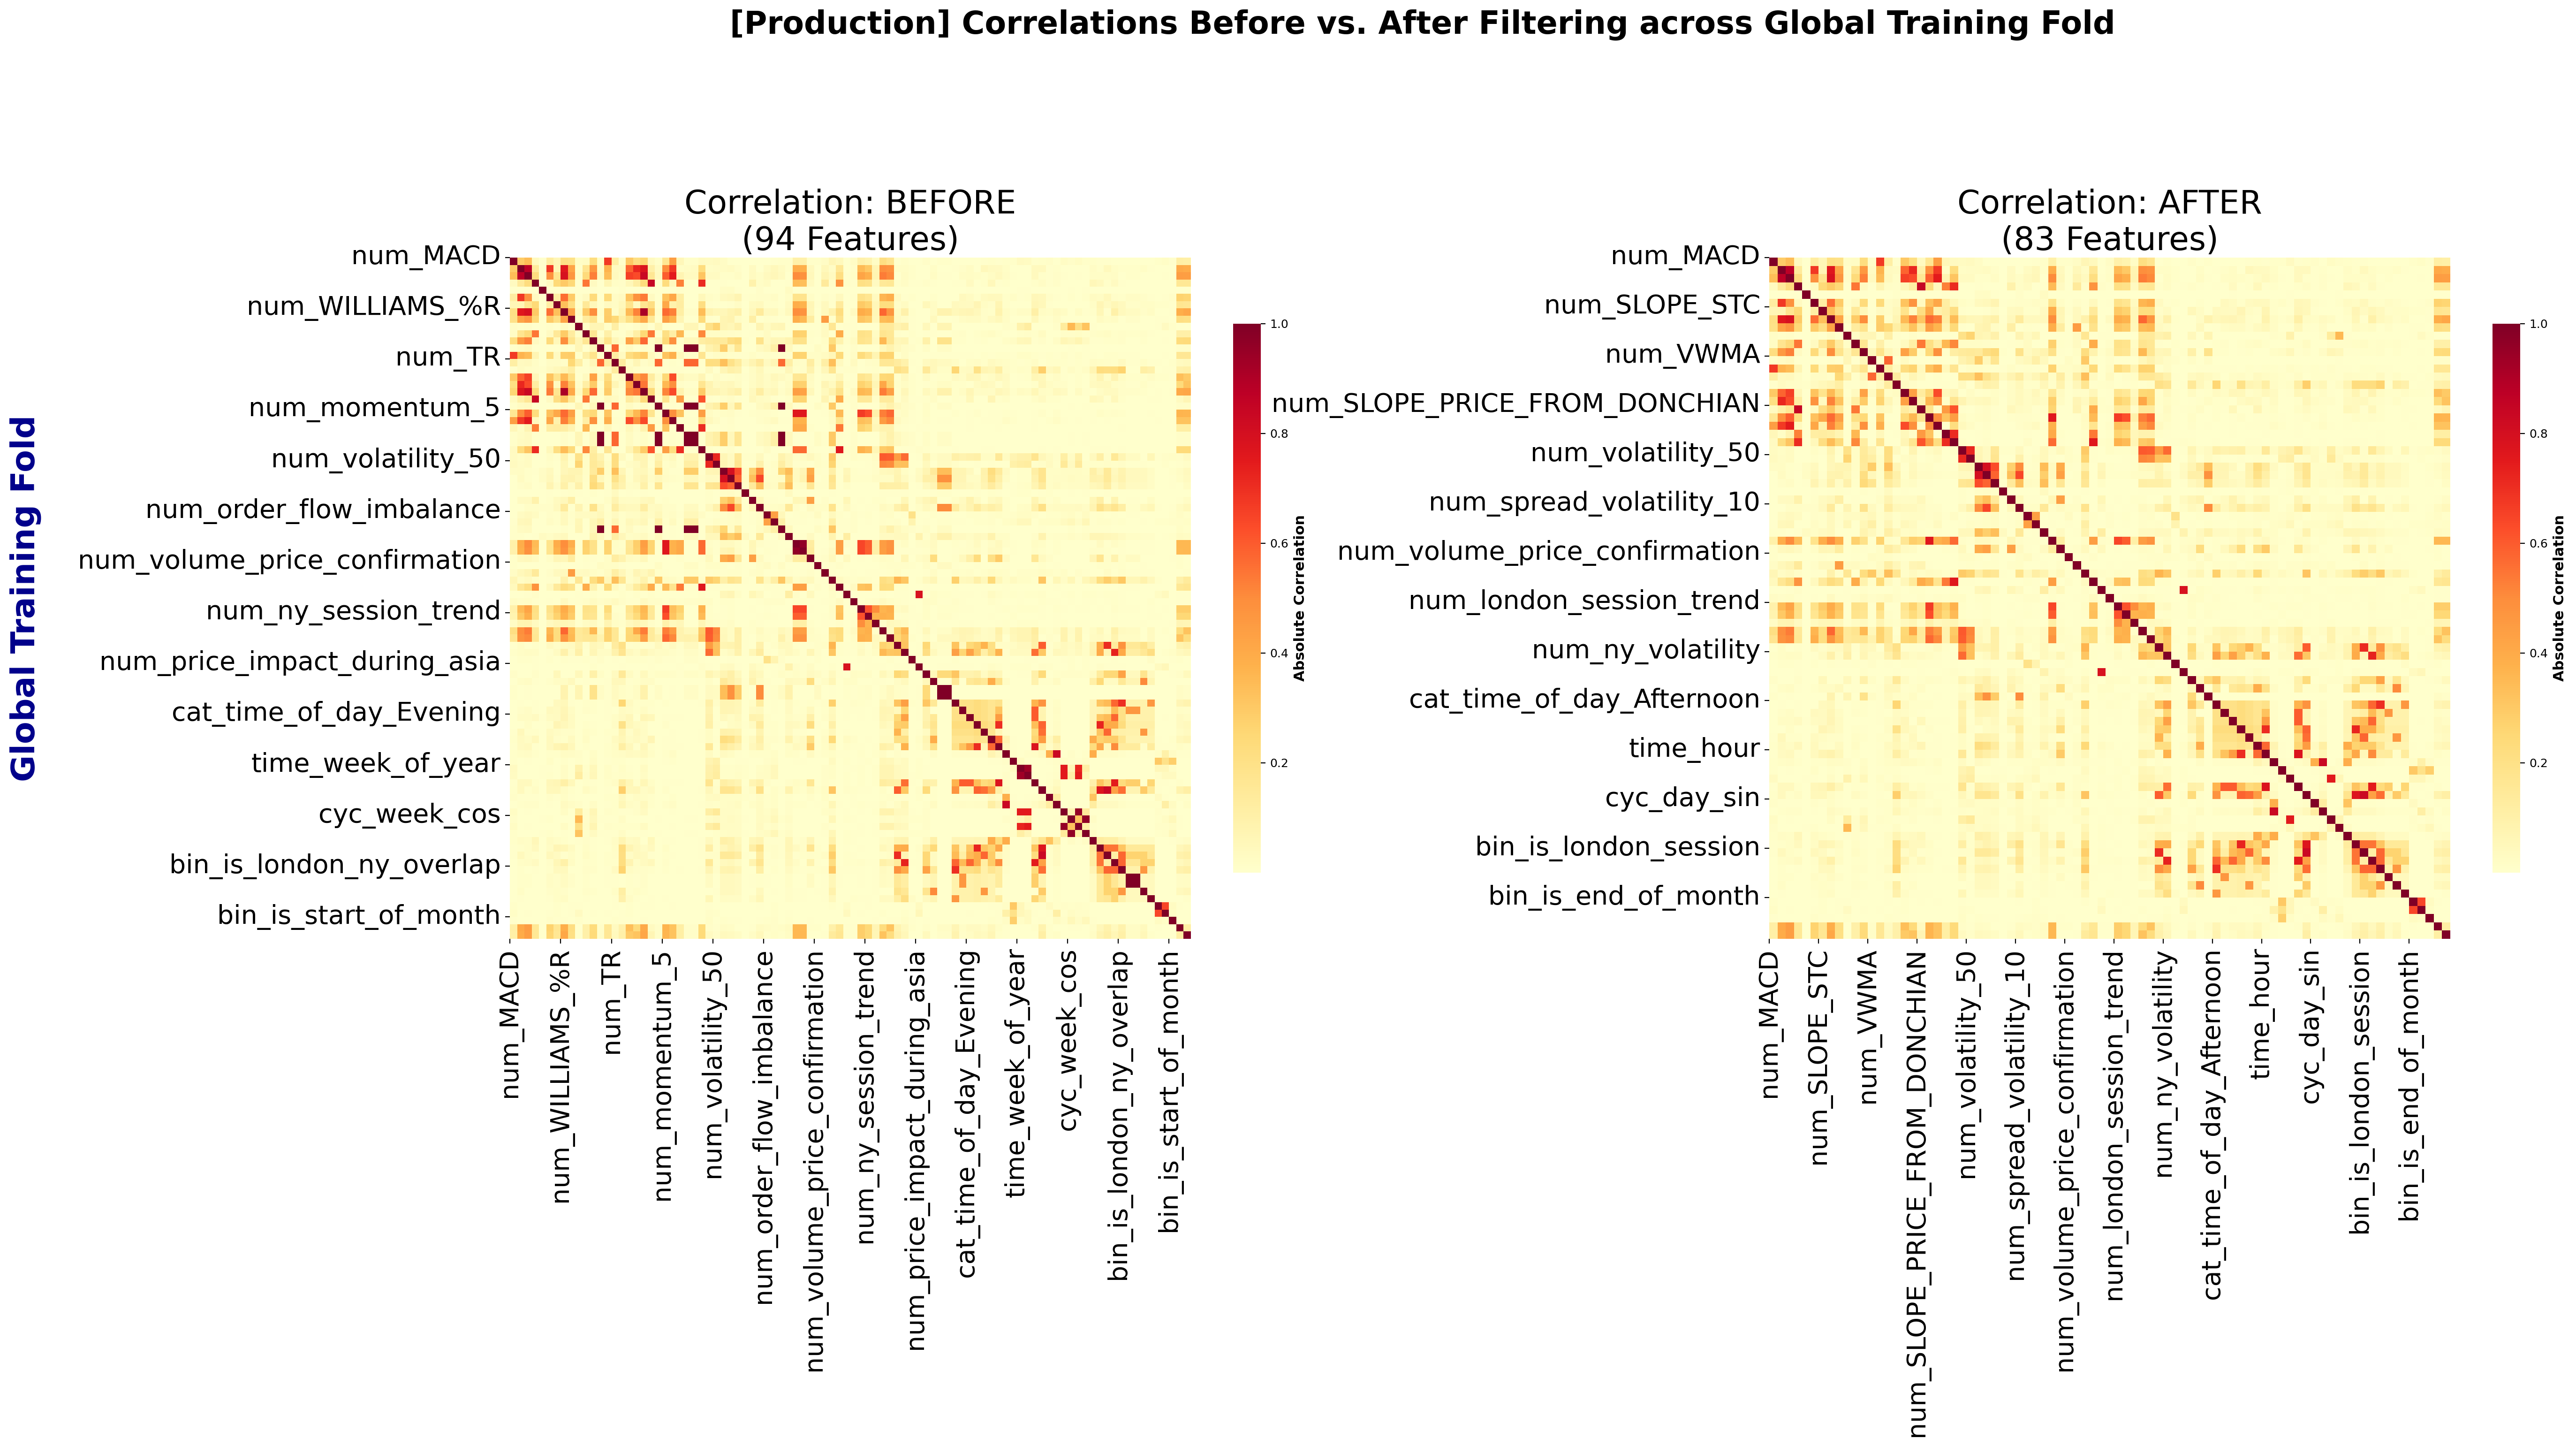
\includegraphics[width=0.95\linewidth]{../data/figures/feature_selection/Production_nested_correlation_heatmap.png}
    \caption{Correlation Filtering During Production}
    \label{fig:prod corr filter}
\end{figure}

\begin{figure}[H]
    \centering
    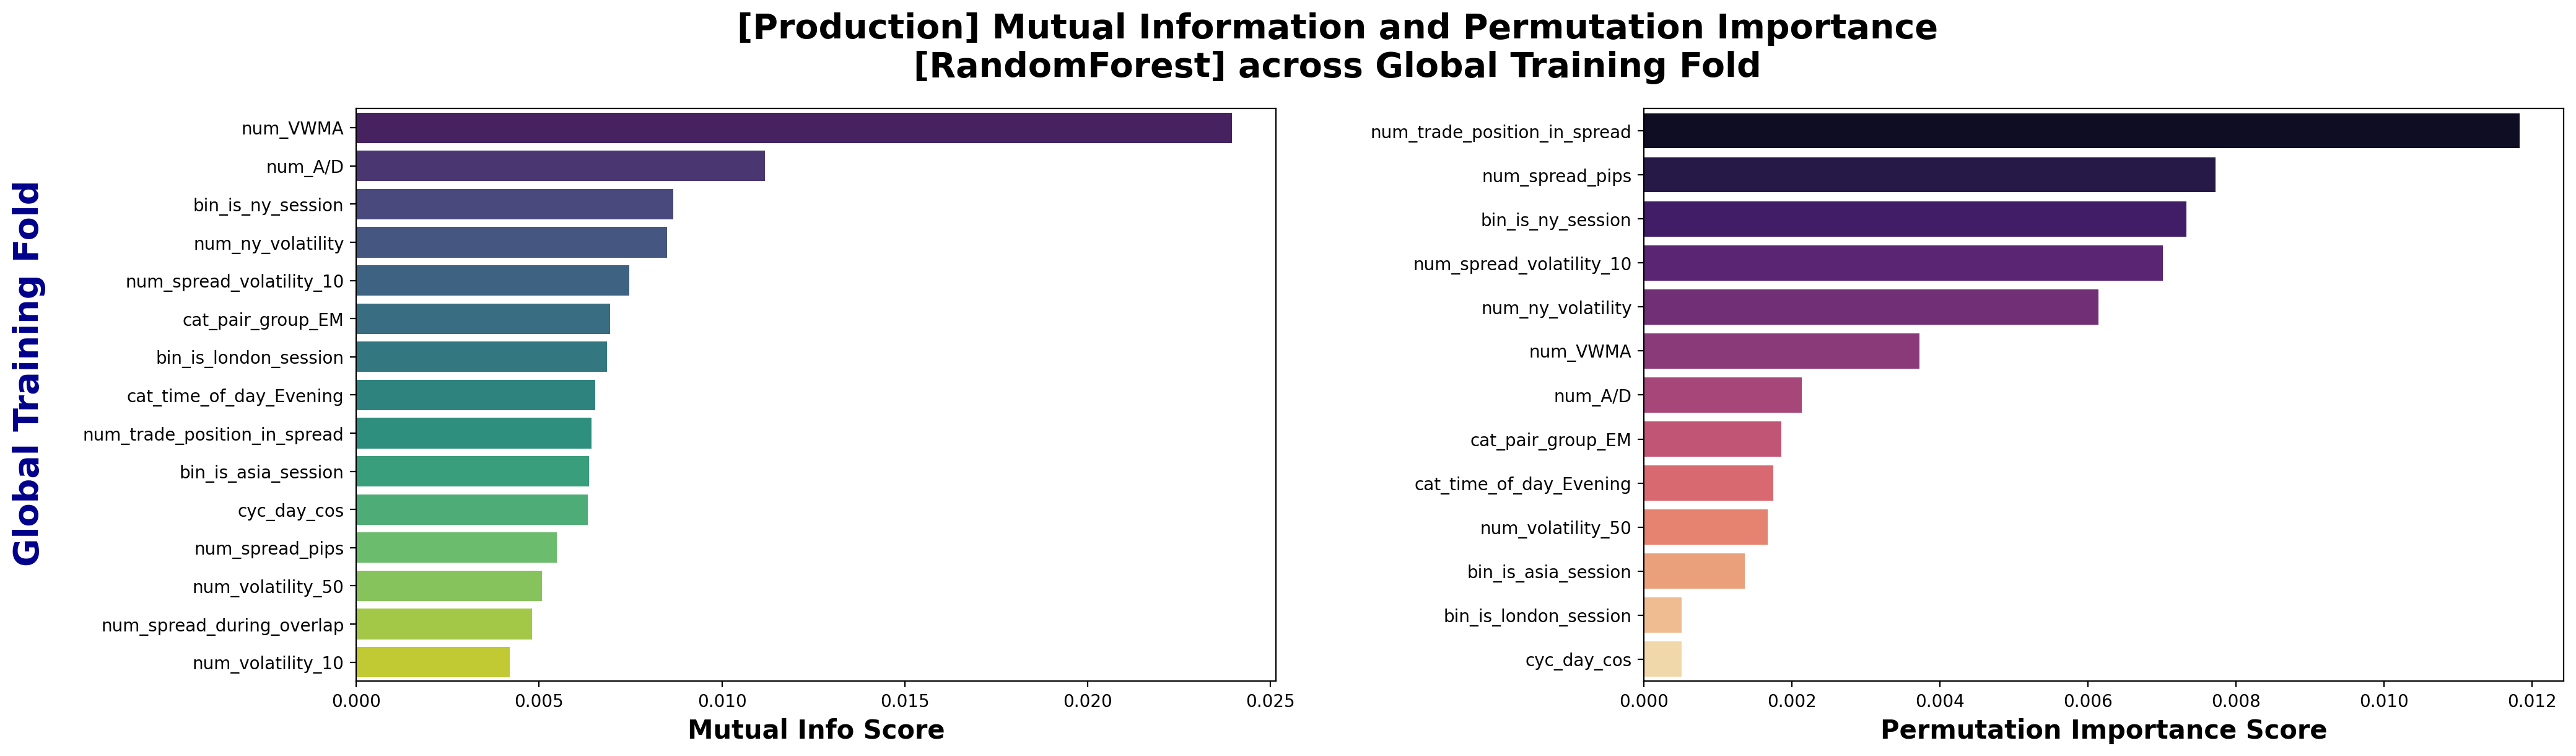
\includegraphics[width=0.95\linewidth]{../data/figures/feature_selection/Production_nested_feature_importances_RandomForest.png}
    \caption{Feature Importances During Production}
    \label{fig:prod featimp filter}
\end{figure}


\subsection{Production Model-Trading Parameter Cascade}

\begin{figure}[H]
    \centering
    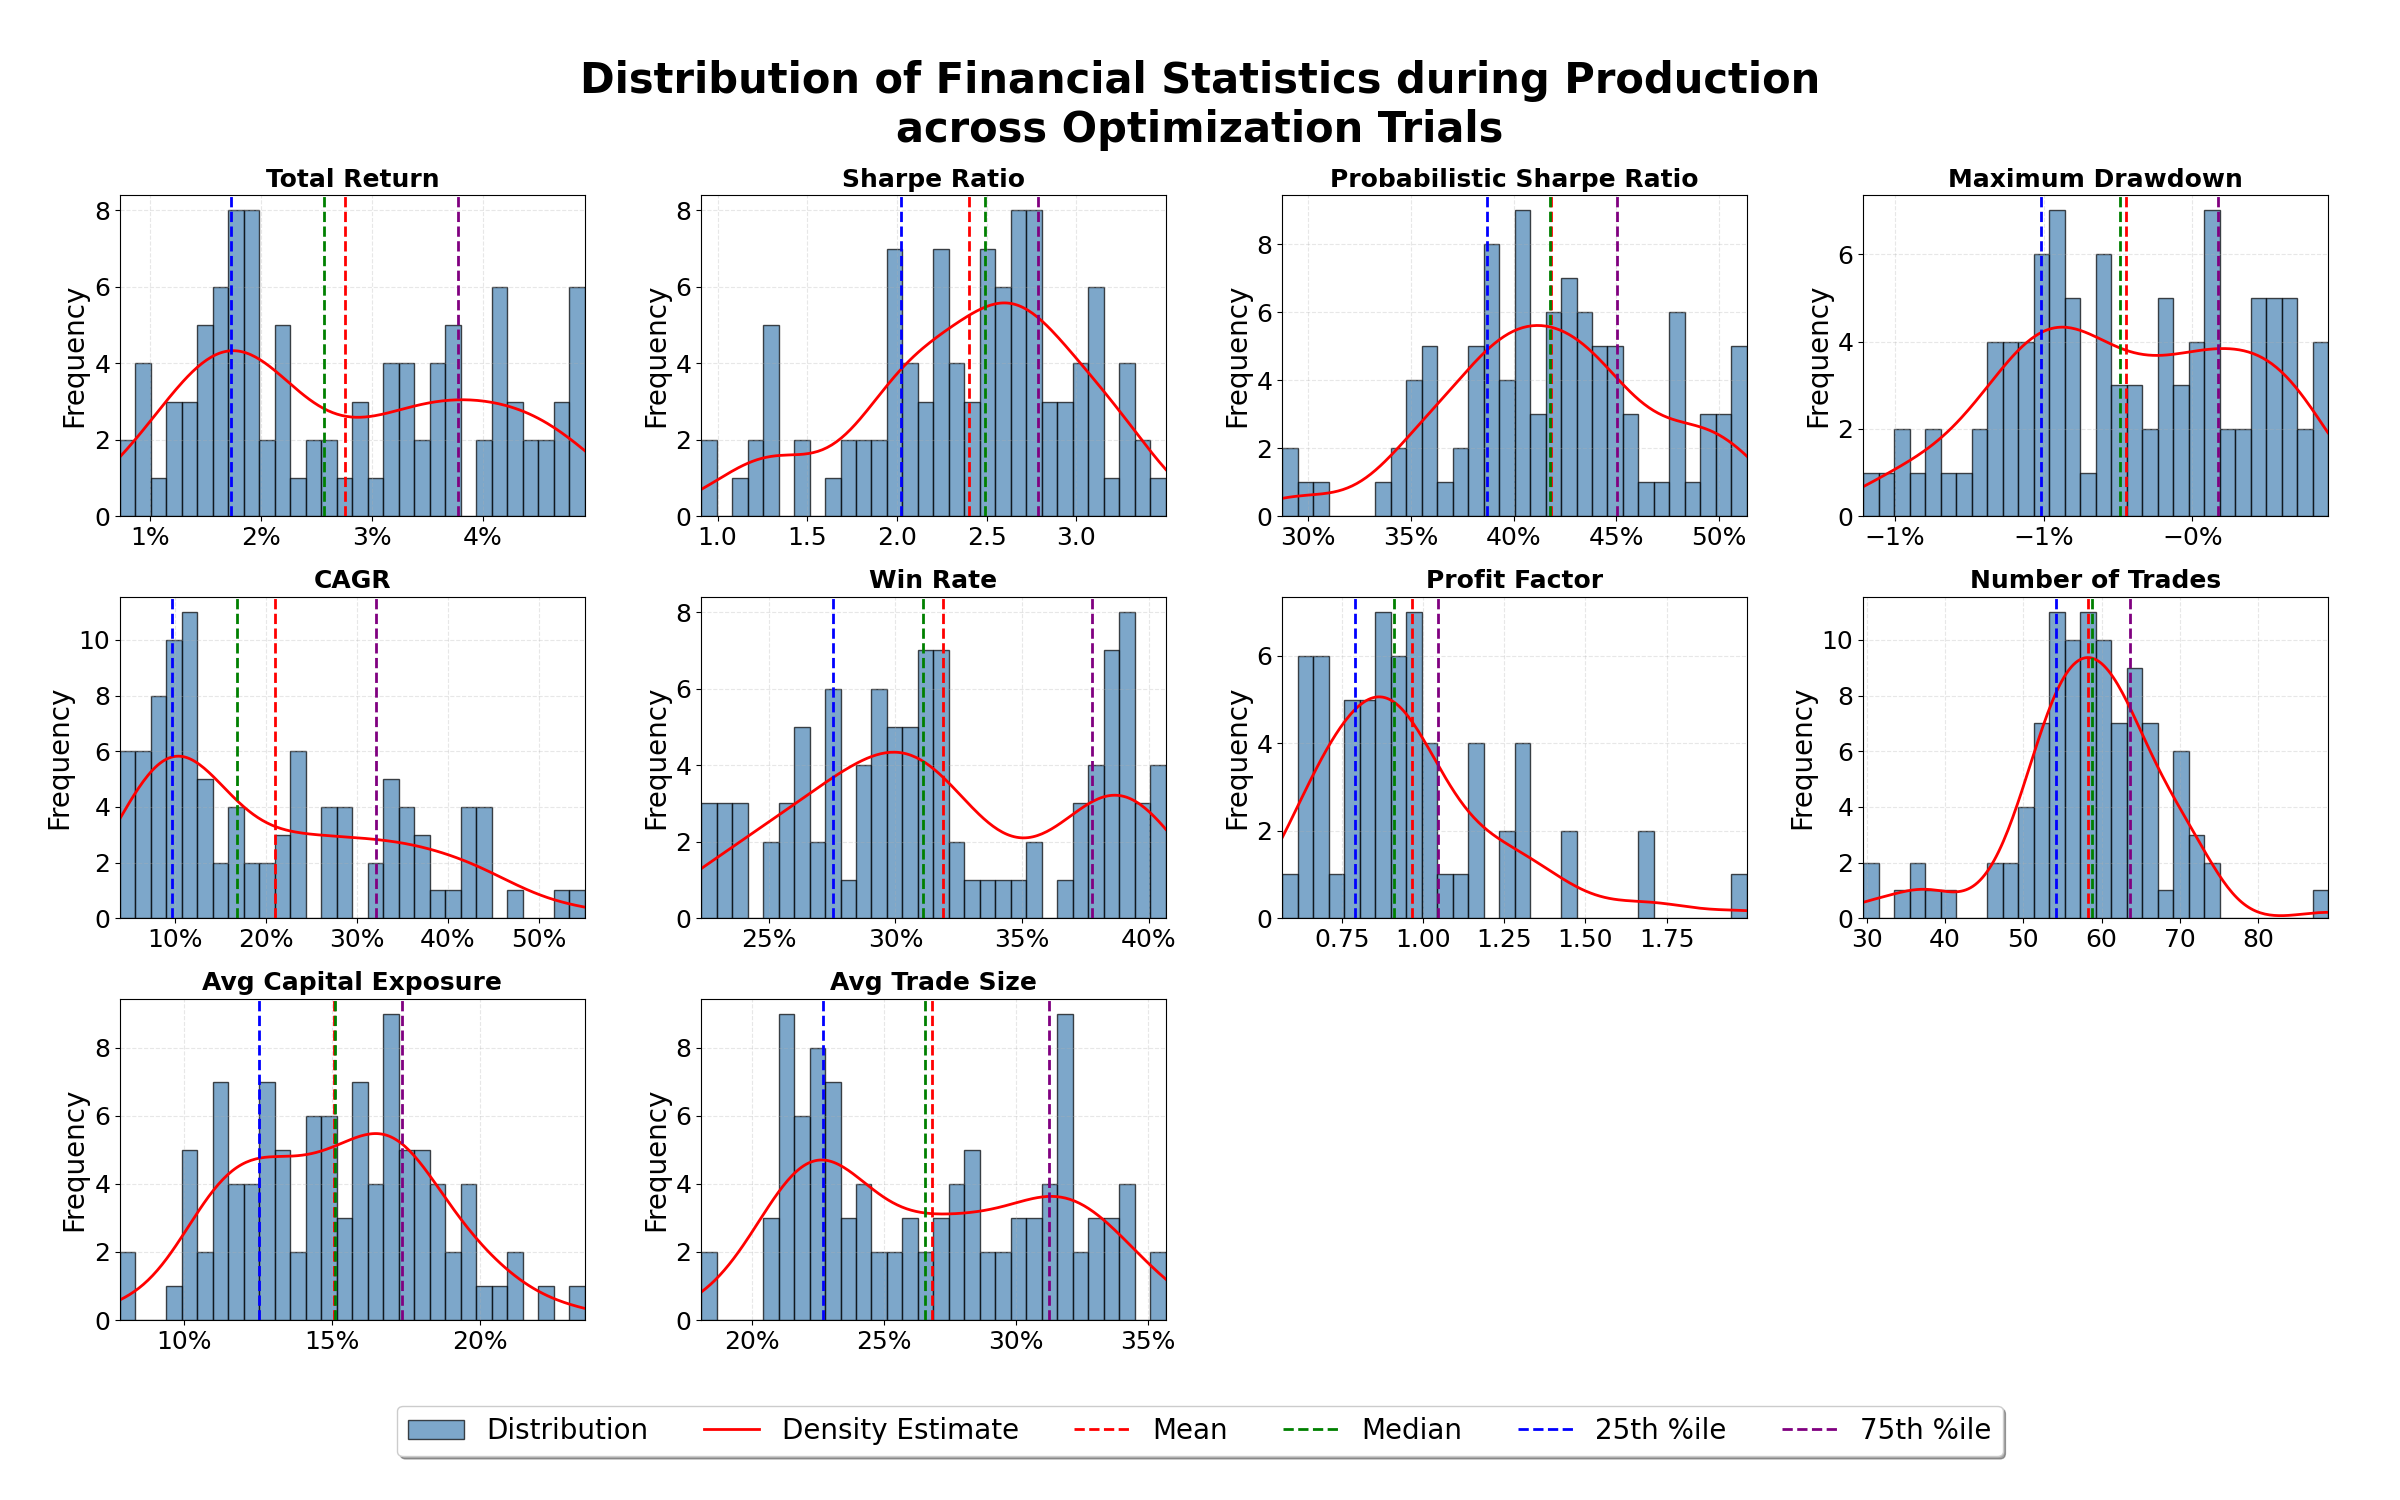
\includegraphics[width=0.95\linewidth]{../data/figures/optimization/distributions/Production_financial_dist_RandomForest.png}
    \caption{Financial Statistic Distributions During Production Optimization}
    \label{fig:prod stat distributions}
\end{figure}

\begin{figure}[H]
    \centering
    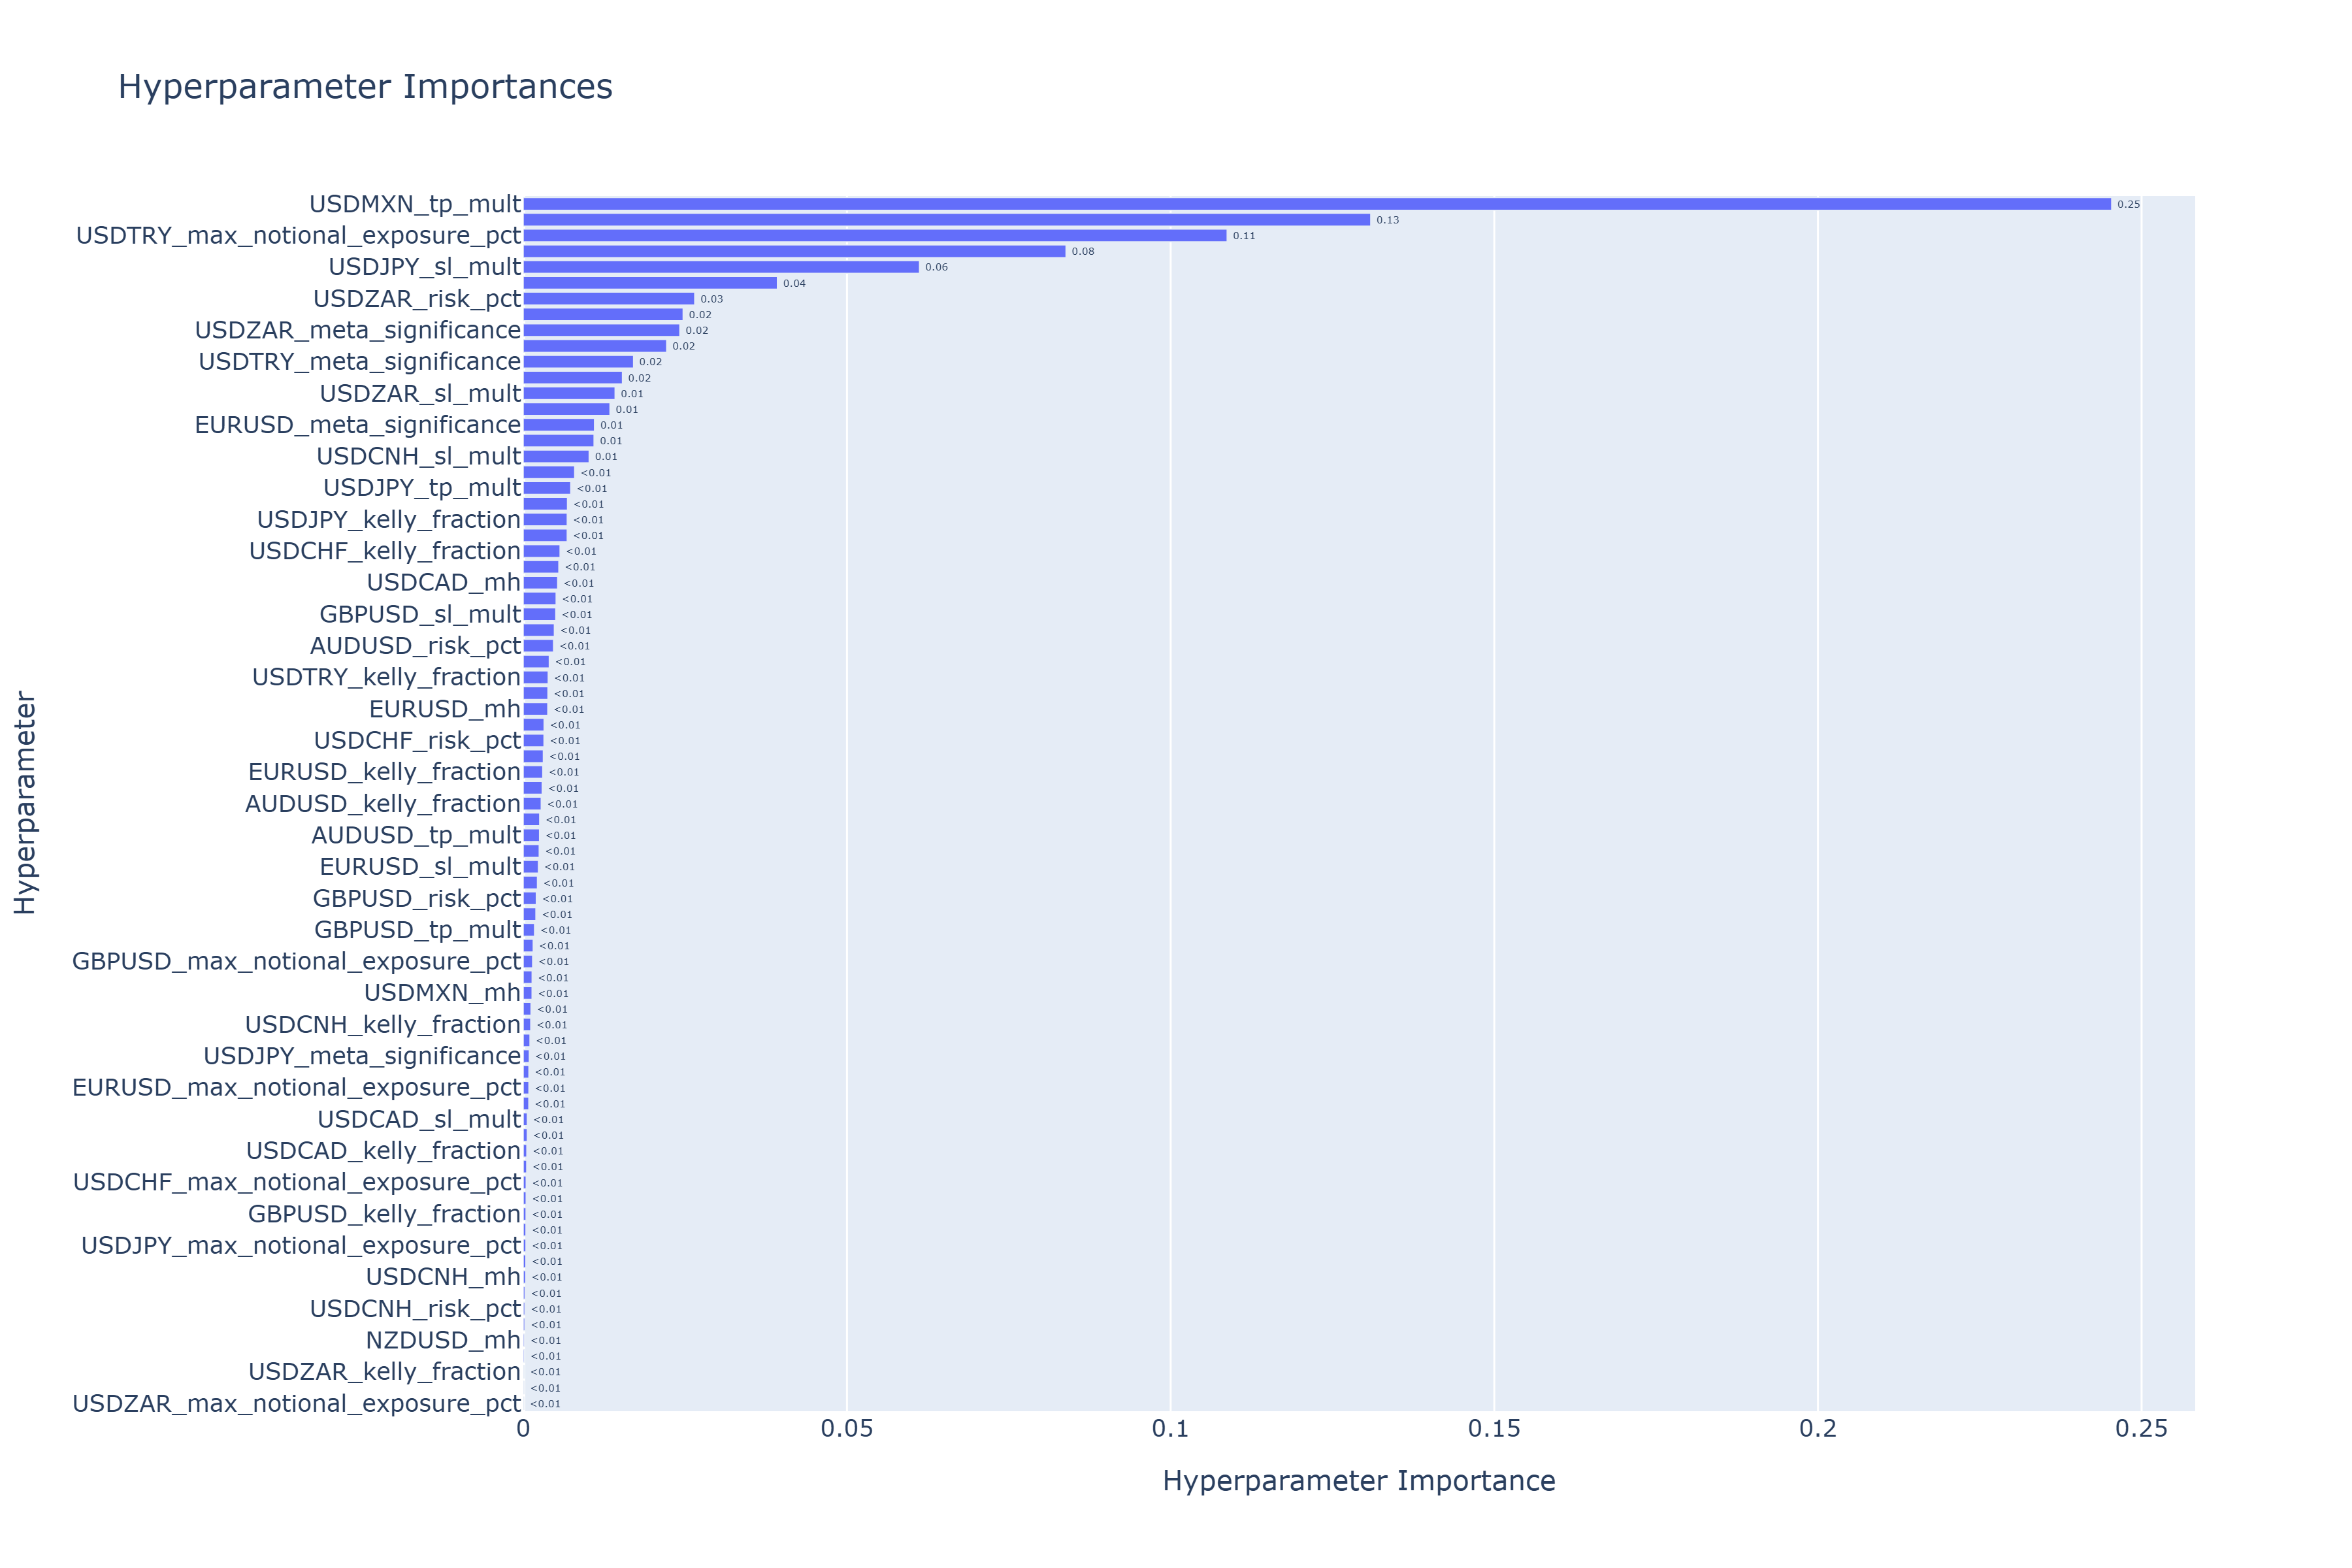
\includegraphics[width=0.95\linewidth]{../data/figures/optimization/production/RandomForest/param_importance_trading_(best)_randomforest.png}
    \caption{Optimization Parameter Importance Trading (Best) RandomForest}
    \label{fig:opt param importance trading rf}
\end{figure}


\subsection{Conformal Filtering}

\begin{figure}[H]
    \centering
    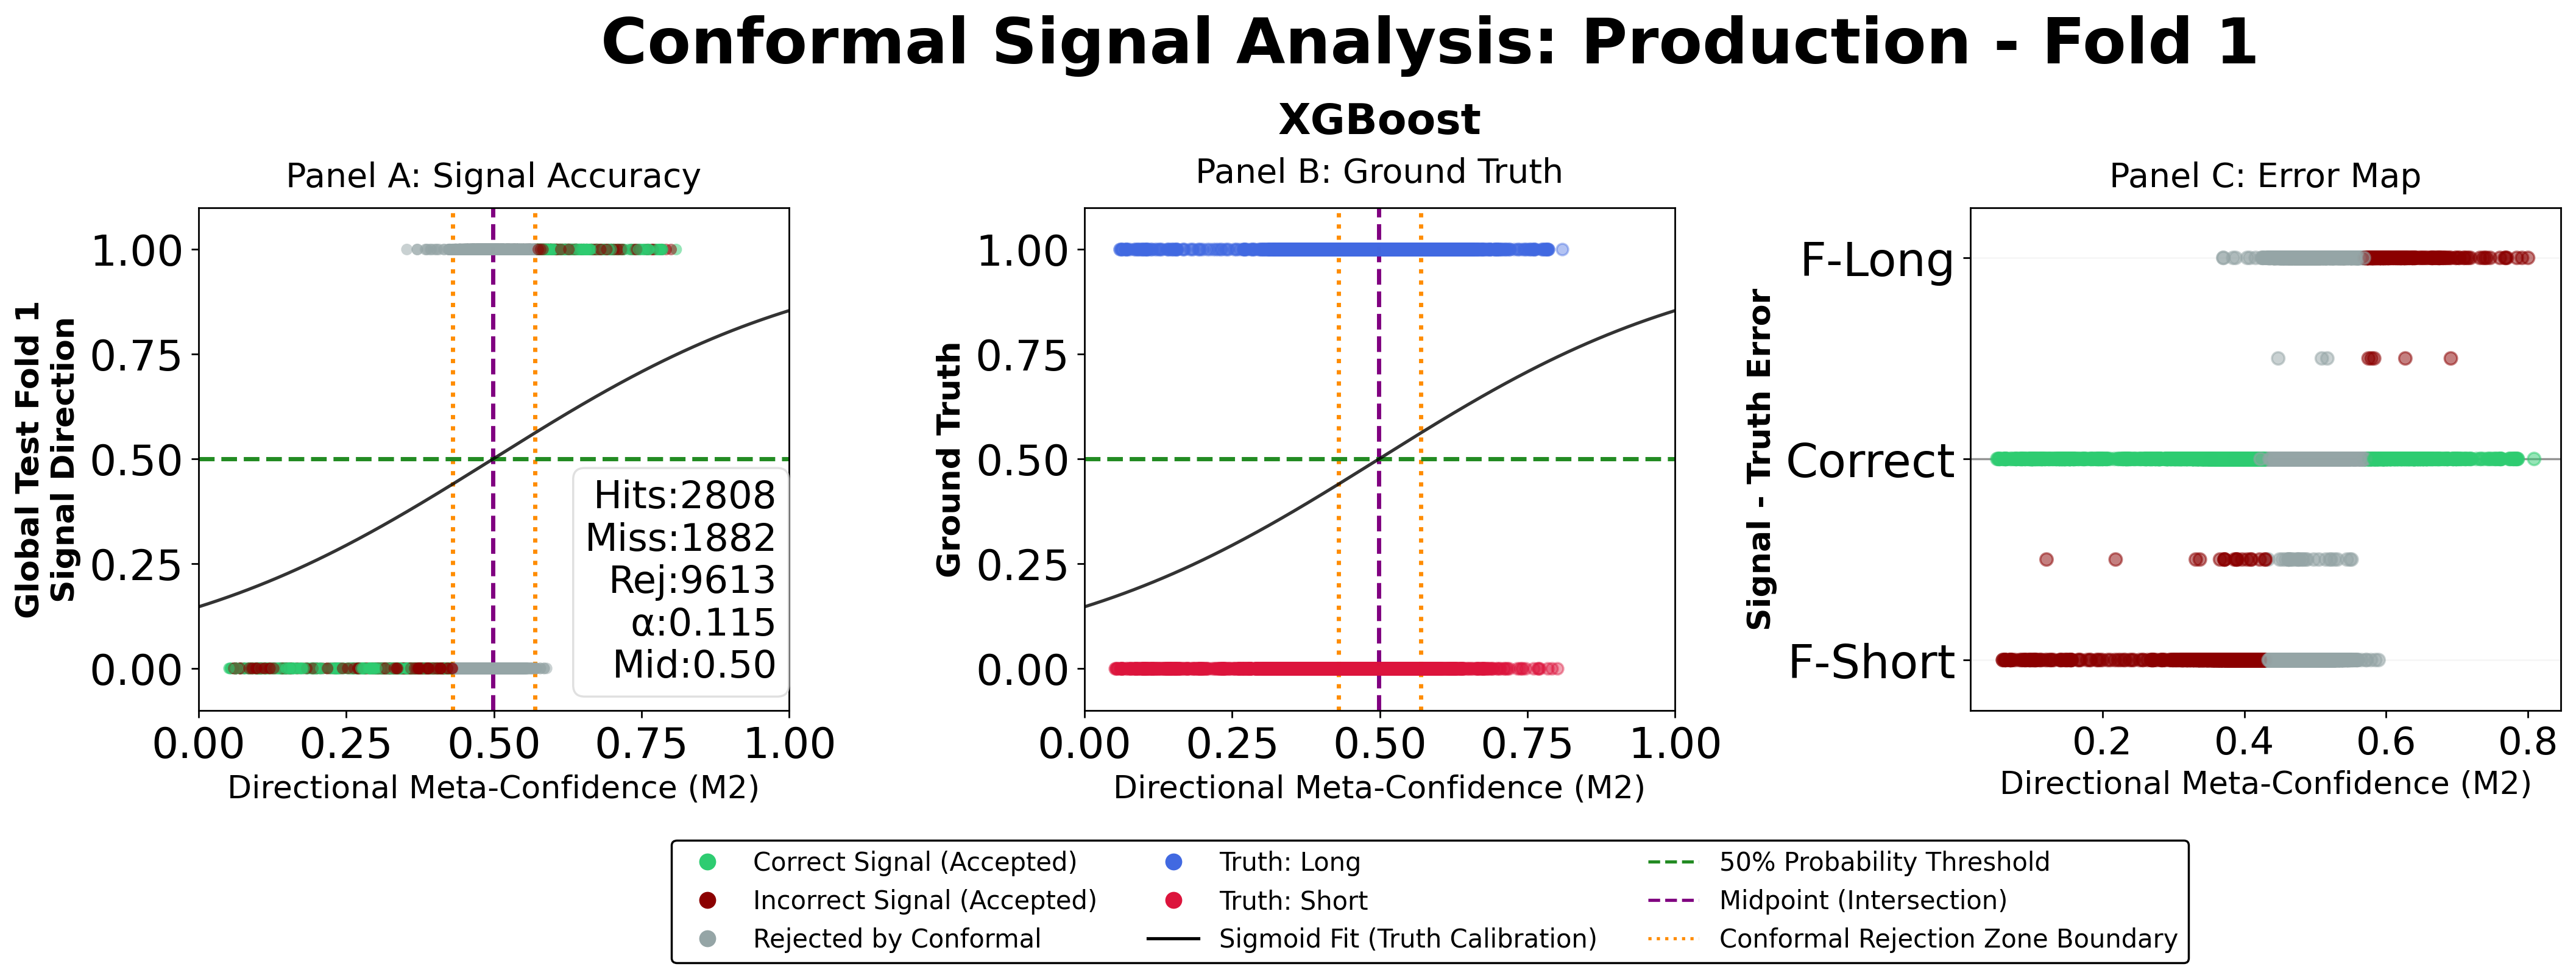
\includegraphics[width=0.7\linewidth]{../data/figures/conformal_predictions/Production_conformal_predictions.png}
    \caption{Model-Specific Conformal Filtering During Production}
    \label{fig:prod conf preds}
\end{figure}


\subsection{Confusion Matrices}

\begin{figure}[H]
    \centering
    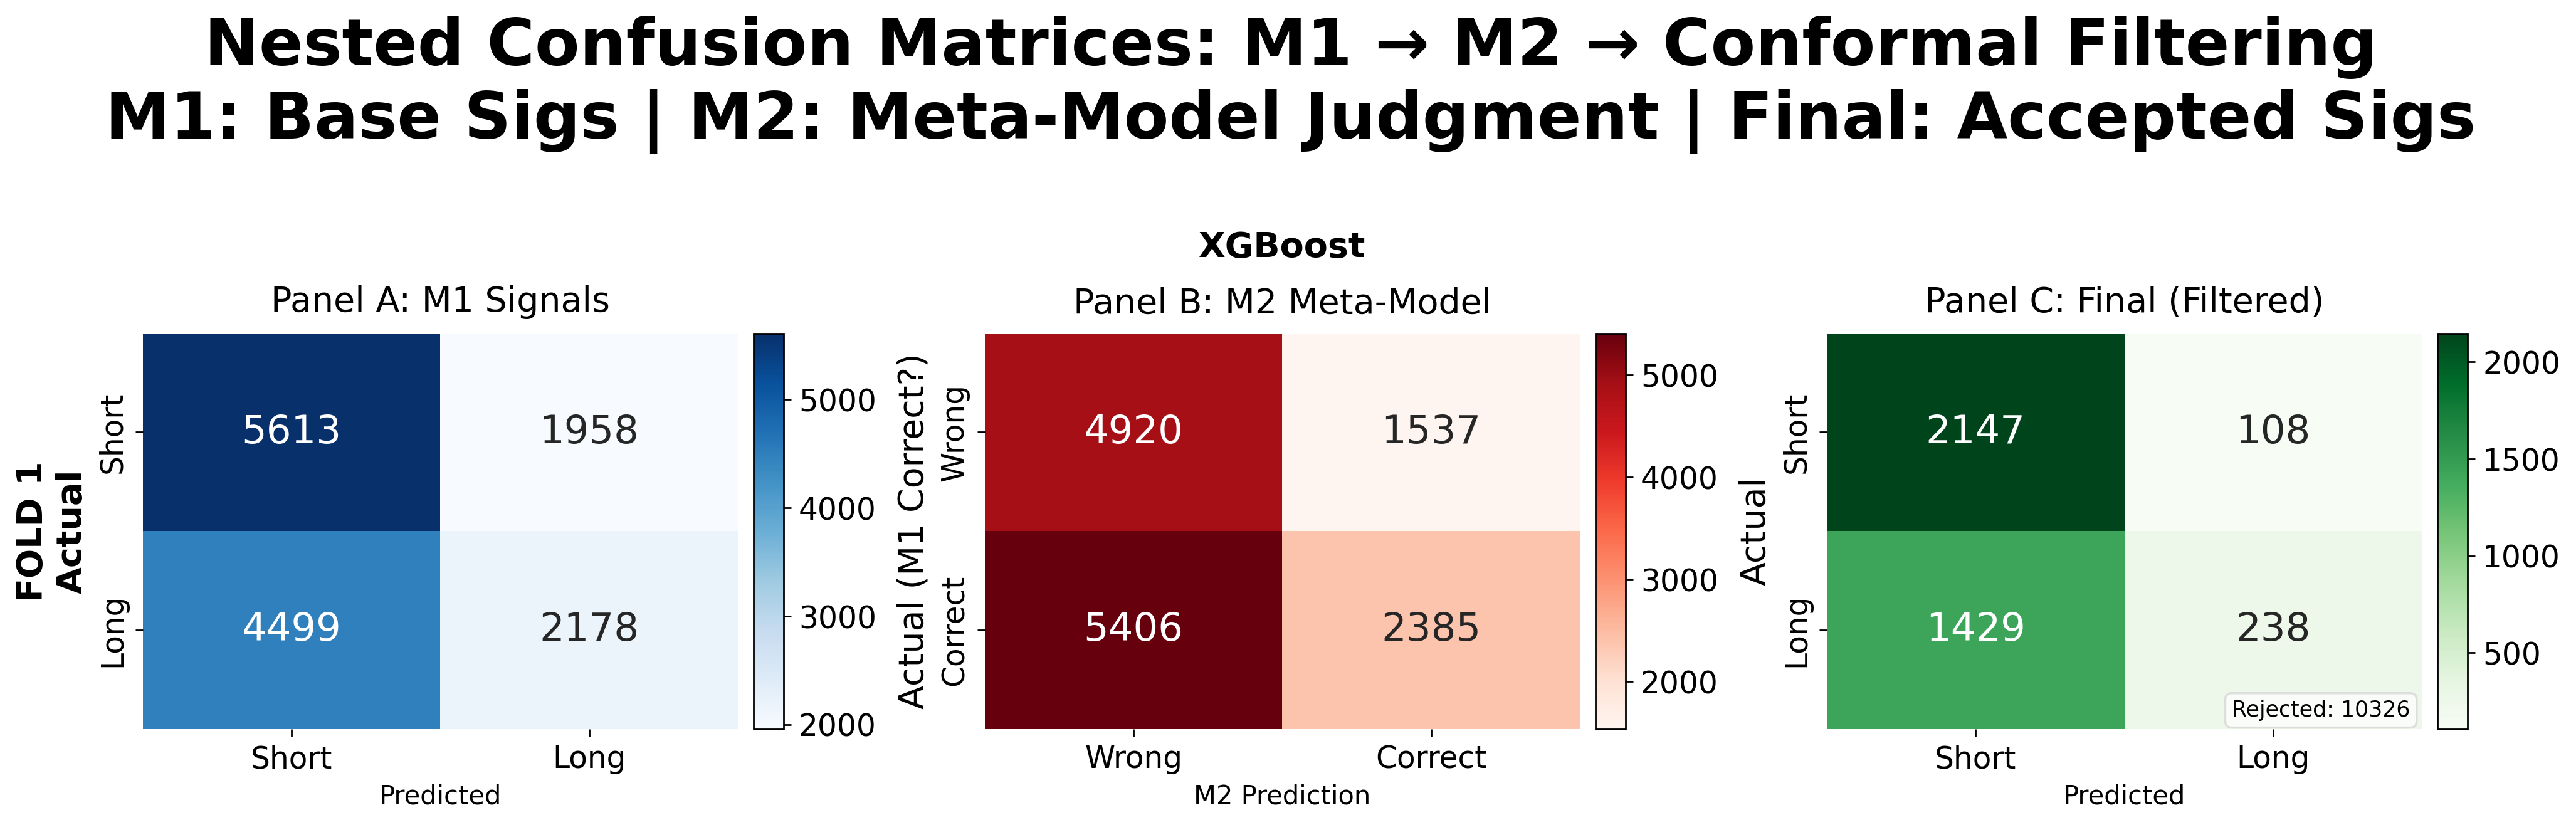
\includegraphics[width=0.95\linewidth]{../data/figures/confusion_matrices/Production_nested_confusion_matrices.png}
    \caption{Model-Specific Confusion Matrices During Production}
    \label{fig:prod confusion matrices}
\end{figure}

\subsection{Reliability Diagrams}

\begin{figure}[H]
    \centering
    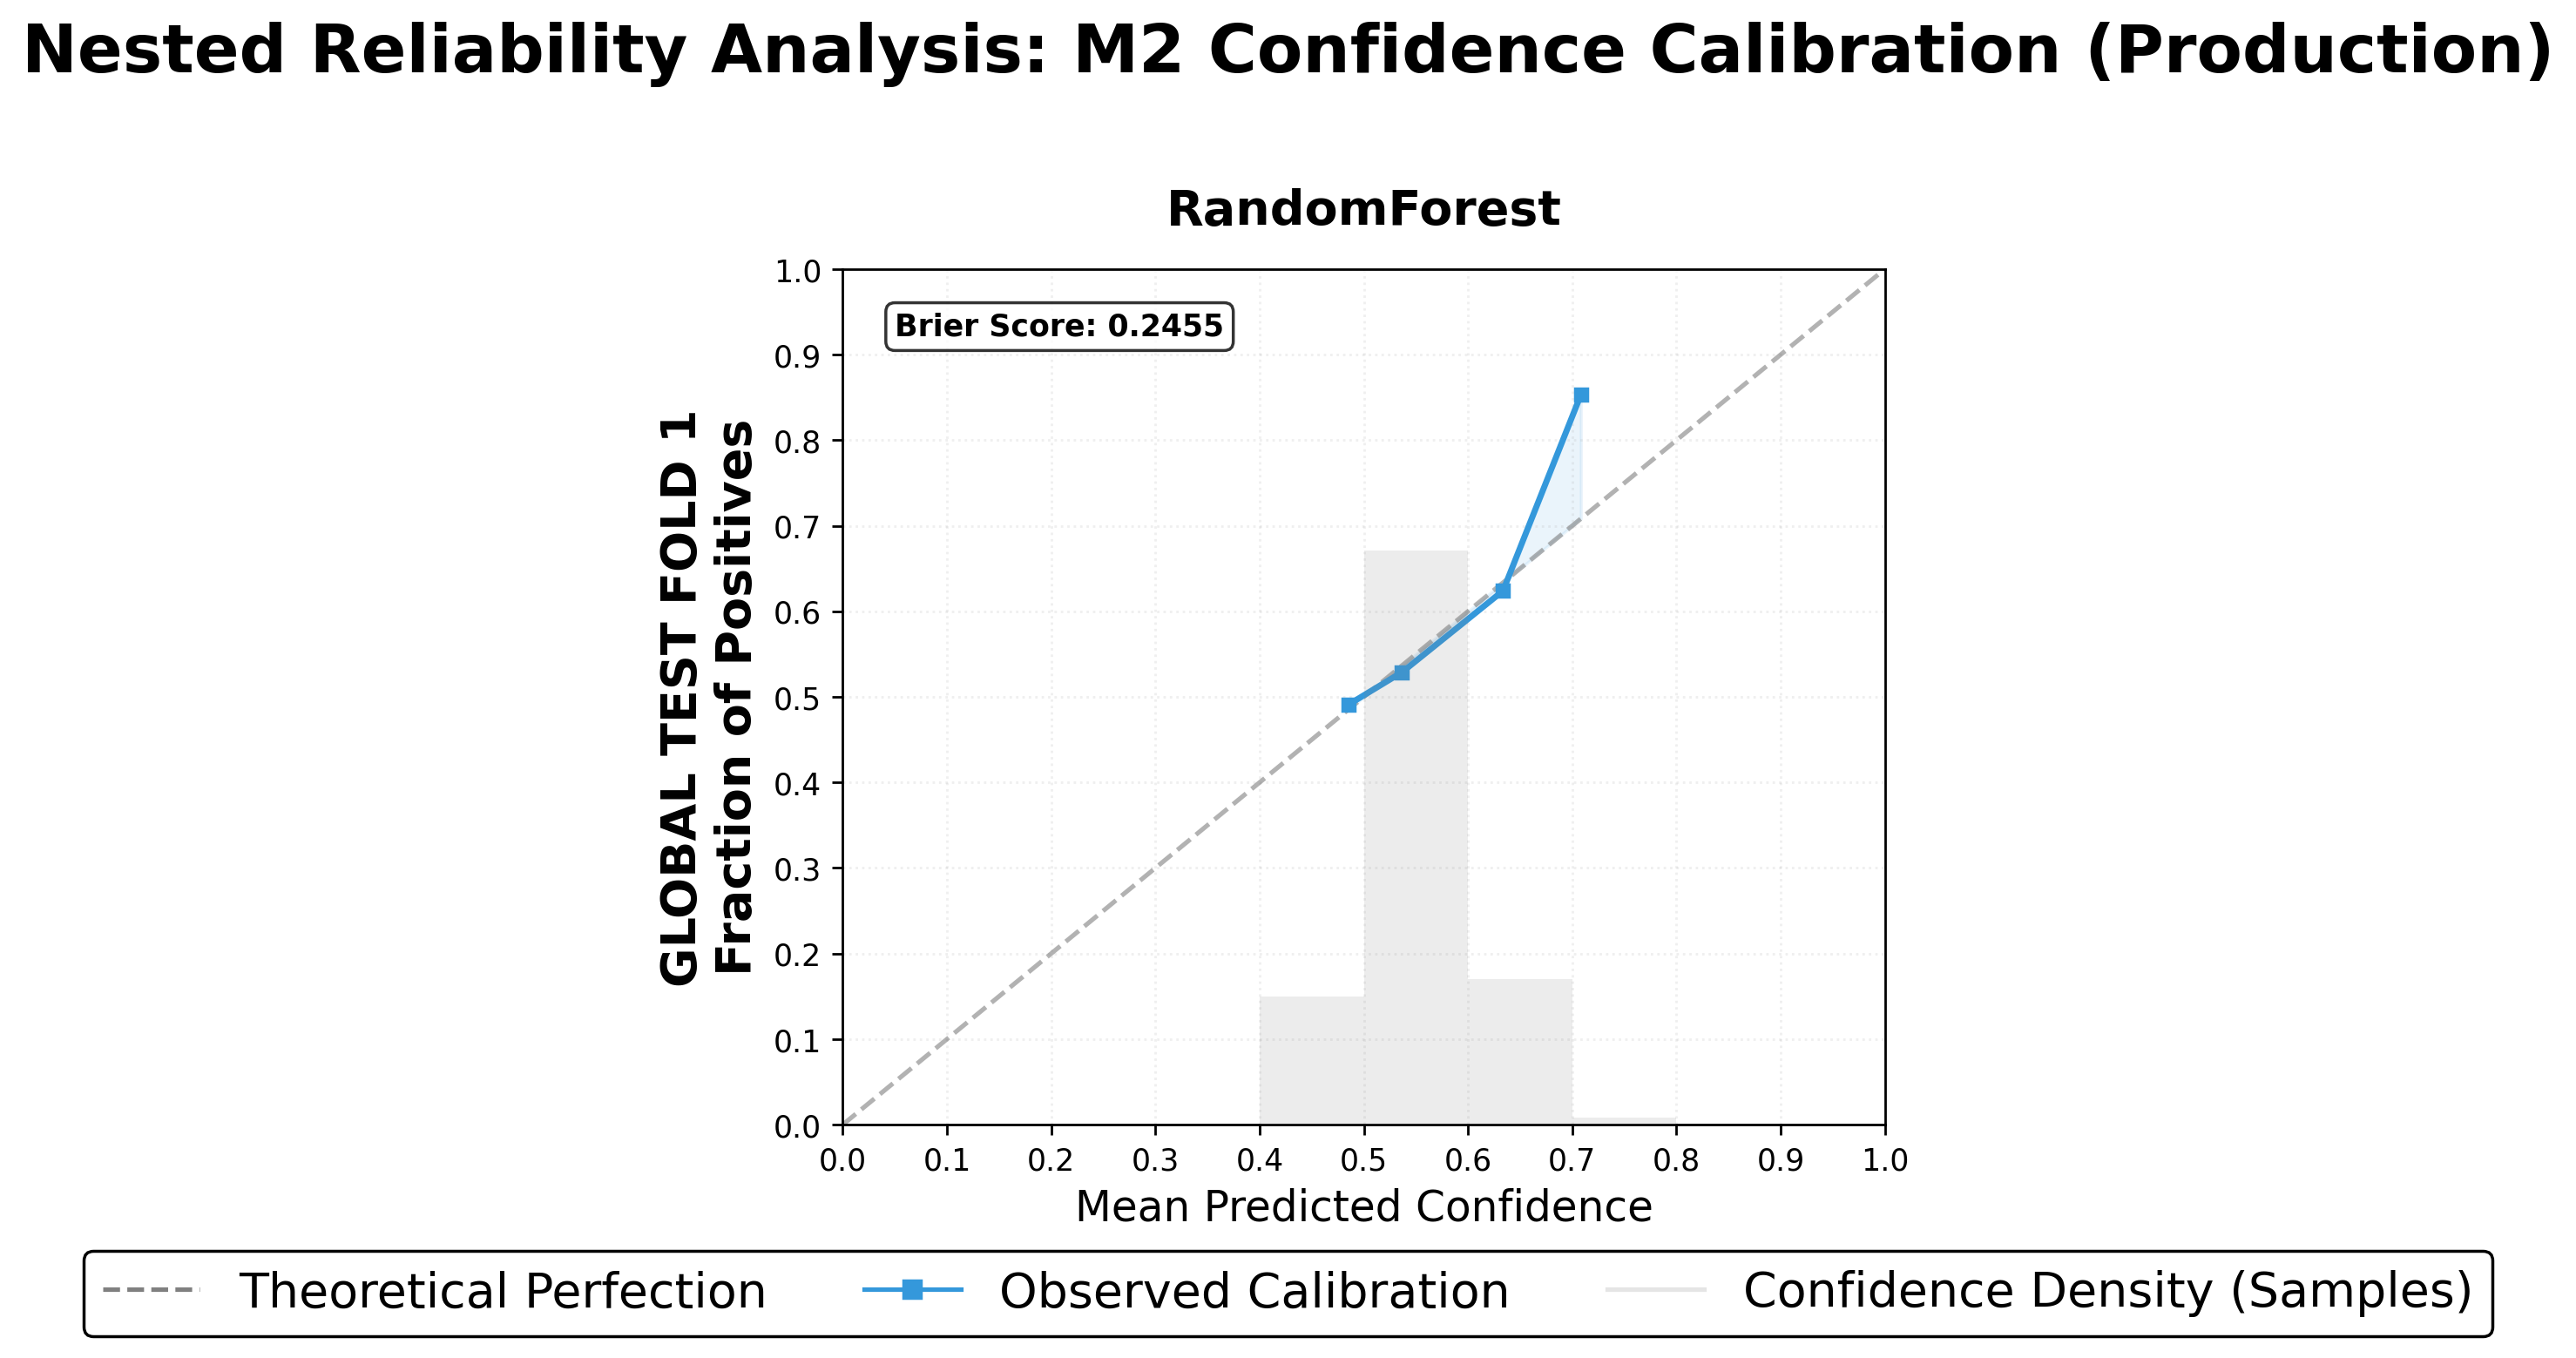
\includegraphics[width=0.5\linewidth]{../data/figures/reliability_diagrams/Production_reliability_diagrams.png}
    \caption{Model-Specific Reliability Diagrams During Production}
    \label{fig:prod reliability curves}
\end{figure}


\section{Miscellaneous}\label{app:miscellaneous}
\subsection{Refactored Codebase}\label{app:code refactored}

\begin{sidewaysfigure}[htbp]
    \centering
    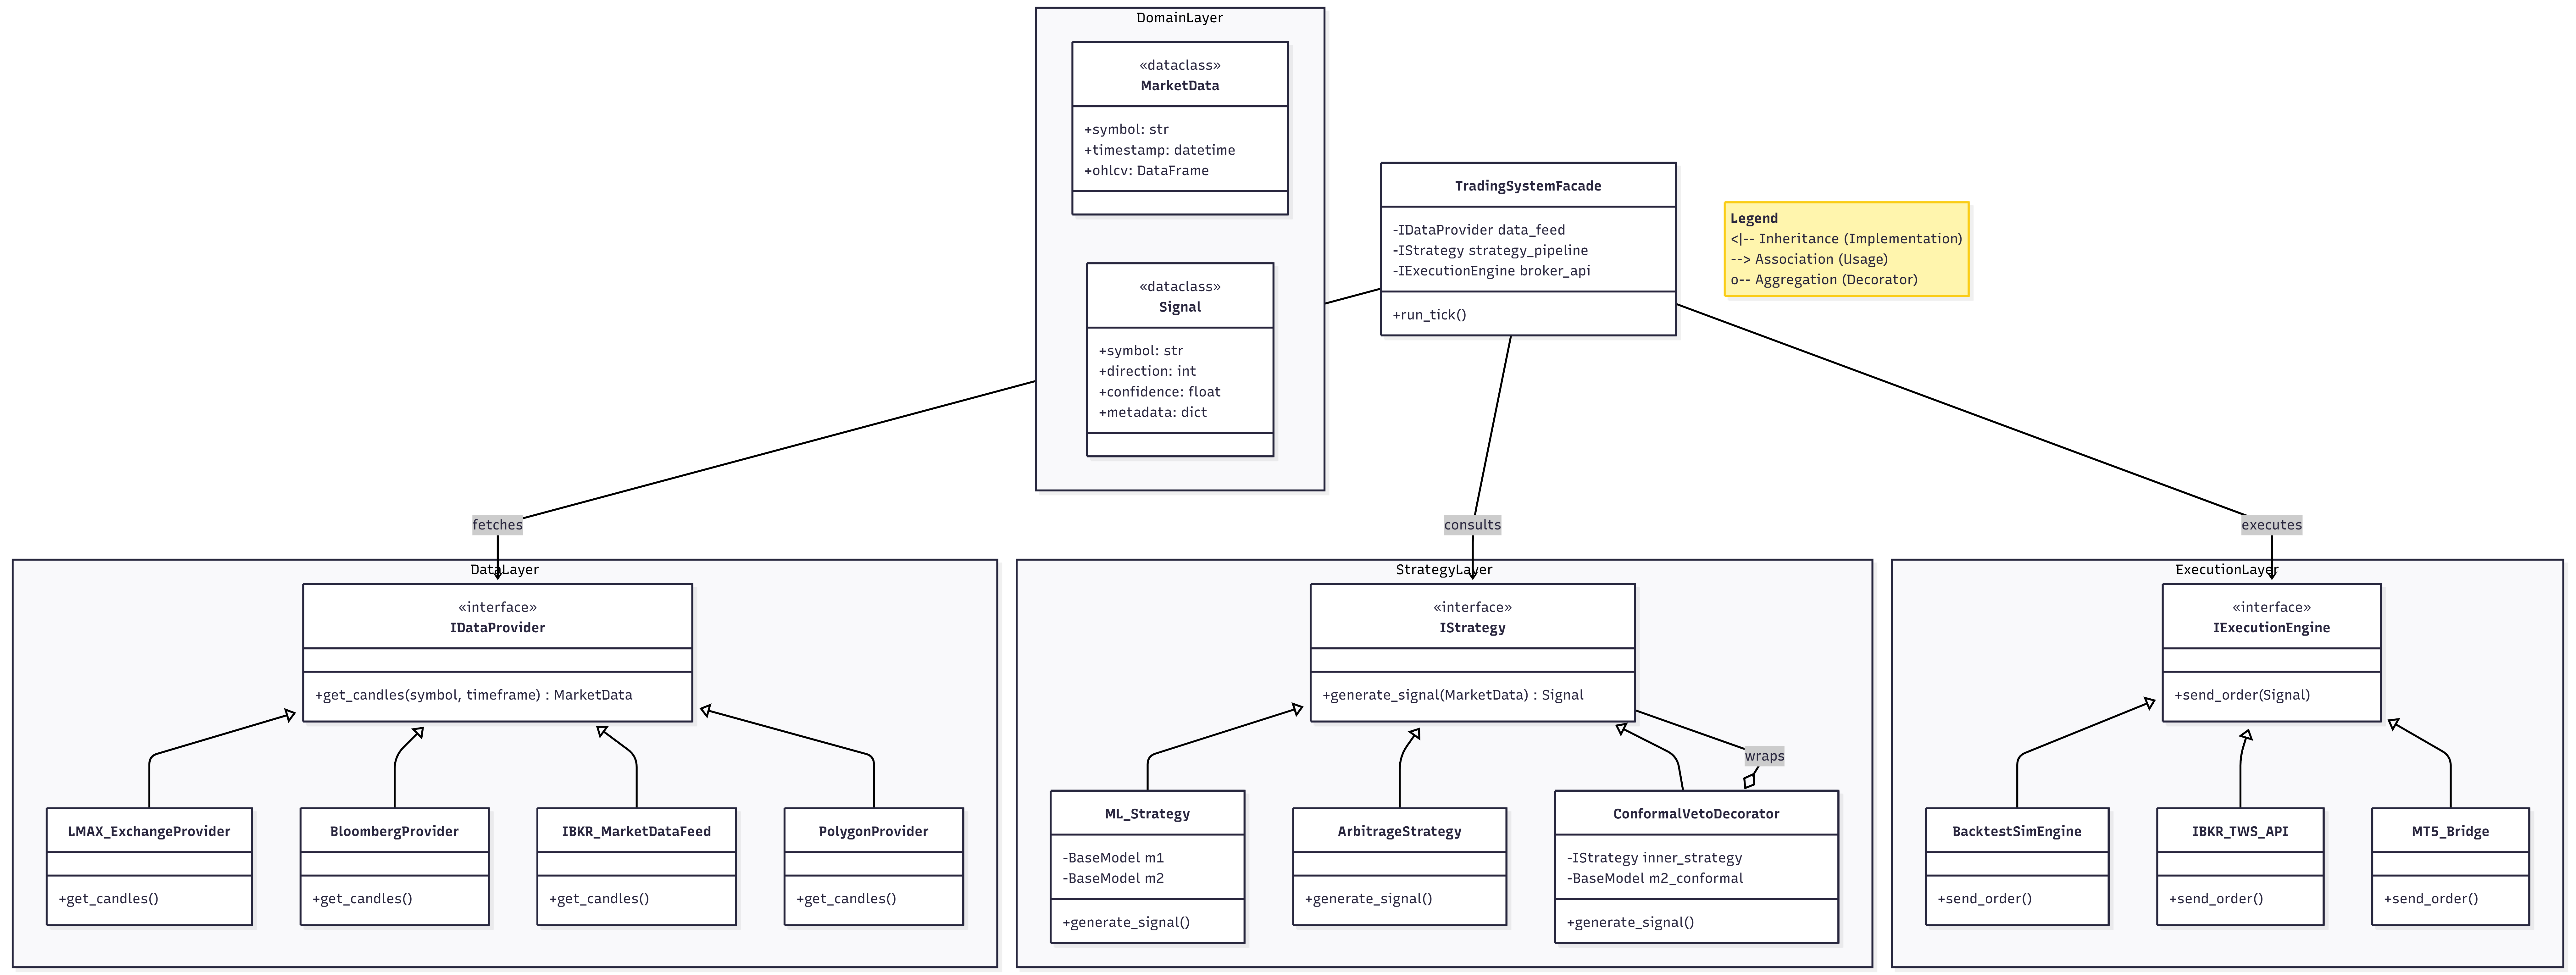
\includegraphics[width=\textheight]{../data/figures/refactored_code/code_refactored.png}
    \caption{Proposed Refactoring of the Codebase}
    \label{fig:refactor}
\end{sidewaysfigure}

\end{document}